\documentclass[twoside]{book}

% Packages required by doxygen
\usepackage{fixltx2e}
\usepackage{calc}
\usepackage{doxygen}
\usepackage[export]{adjustbox} % also loads graphicx
\usepackage{graphicx}
\usepackage[utf8]{inputenc}
\usepackage{makeidx}
\usepackage{multicol}
\usepackage{multirow}
\PassOptionsToPackage{warn}{textcomp}
\usepackage{textcomp}
\usepackage[nointegrals]{wasysym}
\usepackage[table]{xcolor}

% Font selection
\usepackage[T1]{fontenc}
\usepackage[scaled=.90]{helvet}
\usepackage{courier}
\usepackage{amssymb}
\usepackage{sectsty}
\renewcommand{\familydefault}{\sfdefault}
\allsectionsfont{%
  \fontseries{bc}\selectfont%
  \color{darkgray}%
}
\renewcommand{\DoxyLabelFont}{%
  \fontseries{bc}\selectfont%
  \color{darkgray}%
}
\newcommand{\+}{\discretionary{\mbox{\scriptsize$\hookleftarrow$}}{}{}}

% Page & text layout
\usepackage{geometry}
\geometry{%
  a4paper,%
  top=2.5cm,%
  bottom=2.5cm,%
  left=2.5cm,%
  right=2.5cm%
}
\tolerance=750
\hfuzz=15pt
\hbadness=750
\setlength{\emergencystretch}{15pt}
\setlength{\parindent}{0cm}
\setlength{\parskip}{3ex plus 2ex minus 2ex}
\makeatletter
\renewcommand{\paragraph}{%
  \@startsection{paragraph}{4}{0ex}{-1.0ex}{1.0ex}{%
    \normalfont\normalsize\bfseries\SS@parafont%
  }%
}
\renewcommand{\subparagraph}{%
  \@startsection{subparagraph}{5}{0ex}{-1.0ex}{1.0ex}{%
    \normalfont\normalsize\bfseries\SS@subparafont%
  }%
}
\makeatother

% Headers & footers
\usepackage{fancyhdr}
\pagestyle{fancyplain}
\fancyhead[LE]{\fancyplain{}{\bfseries\thepage}}
\fancyhead[CE]{\fancyplain{}{}}
\fancyhead[RE]{\fancyplain{}{\bfseries\leftmark}}
\fancyhead[LO]{\fancyplain{}{\bfseries\rightmark}}
\fancyhead[CO]{\fancyplain{}{}}
\fancyhead[RO]{\fancyplain{}{\bfseries\thepage}}
\fancyfoot[LE]{\fancyplain{}{}}
\fancyfoot[CE]{\fancyplain{}{}}
\fancyfoot[RE]{\fancyplain{}{\bfseries\scriptsize Generated by Doxygen }}
\fancyfoot[LO]{\fancyplain{}{\bfseries\scriptsize Generated by Doxygen }}
\fancyfoot[CO]{\fancyplain{}{}}
\fancyfoot[RO]{\fancyplain{}{}}
\renewcommand{\footrulewidth}{0.4pt}
\renewcommand{\chaptermark}[1]{%
  \markboth{#1}{}%
}
\renewcommand{\sectionmark}[1]{%
  \markright{\thesection\ #1}%
}

% Indices & bibliography
\usepackage{natbib}
\usepackage[titles]{tocloft}
\setcounter{tocdepth}{3}
\setcounter{secnumdepth}{5}
\makeindex

% Hyperlinks (required, but should be loaded last)
\usepackage{ifpdf}
\ifpdf
  \usepackage[pdftex,pagebackref=true]{hyperref}
\else
  \usepackage[ps2pdf,pagebackref=true]{hyperref}
\fi
\hypersetup{%
  colorlinks=true,%
  linkcolor=blue,%
  citecolor=blue,%
  unicode%
}

% Custom commands
\newcommand{\clearemptydoublepage}{%
  \newpage{\pagestyle{empty}\cleardoublepage}%
}

\usepackage{caption}
\captionsetup{labelsep=space,justification=centering,font={bf},singlelinecheck=off,skip=4pt,position=top}

%===== C O N T E N T S =====

\begin{document}

% Titlepage & ToC
\hypersetup{pageanchor=false,
             bookmarksnumbered=true,
             pdfencoding=unicode
            }
\pagenumbering{alph}
\begin{titlepage}
\vspace*{7cm}
\begin{center}%
{\Large Active Manipulation Learning }\\
\vspace*{1cm}
{\large Generated by Doxygen 1.8.12}\\
\end{center}
\end{titlepage}
\clearemptydoublepage
\pagenumbering{roman}
\tableofcontents
\clearemptydoublepage
\pagenumbering{arabic}
\hypersetup{pageanchor=true}

%--- Begin generated contents ---
\chapter{aml}
\label{md__r_e_a_d_m_e}
\hypertarget{md__r_e_a_d_m_e}{}
\subsection*{Live Docs for A\-M\-L}


\begin{DoxyItemize}
\item Live documentation for A\-M\-L can be found \href{https://docs.google.com/document/d/1_xM5TvY-ARBdU3P3D4MrxzcuUbaHkiwEP5UDHMdy4yM/edit?usp=sharing}{\tt here}
\item Also see the docs folder in the A\-M\-L root directory for the doxygen documentation.
\end{DoxyItemize}

\subsection*{Setting up A\-M\-L -\/ The Very Simple Way}


\begin{DoxyItemize}
\item A set of scripts for installing A\-M\-L natively in your host machine, or for getting it setup in a docker container can be found \href{https://github.com/eaa3/aml_install}{\tt here}
\end{DoxyItemize}

\subsection*{Setting A\-M\-L manually}

\subsubsection*{Dependencies}


\begin{DoxyItemize}
\item \href{http://wiki.ros.org/indigo/Installation/Ubuntu}{\tt R\-O\-S (Indigo)}
\item \href{http://sdk.rethinkrobotics.com/wiki/Hello_Baxter}{\tt Baxter\-S\-D\-K}
\item \href{http://sdk.rethinkrobotics.com/wiki/Simulator_Installation}{\tt Baxter Simulator}
\item \href{http://sdk.rethinkrobotics.com/intera/Main_Page}{\tt Saywer Robot}
\end{DoxyItemize}

\paragraph*{Python Libraries}


\begin{DoxyItemize}
\item \href{http://www.numpy.org/}{\tt numpy}
\item \href{https://pypi.python.org/pypi/numpy-quaternion}{\tt numpy-\/quaternion}
\item \href{http://www.pygame.org/download.shtml}{\tt pygame}
\item \href{https://pypi.python.org/pypi/PySide/1.2.4}{\tt Py\-Side}
\item \href{https://github.com/pybox2d/pybox2d}{\tt pybox2d}
\item \href{https://pypi.python.org/pypi/Pillow/4.1.1}{\tt Pillow}
\item \href{https://pypi.python.org/pypi/scipy/0.19.0}{\tt Scipy}
\item \href{https://pandas.pydata.org/}{\tt Pandas}
\item \href{https://pypi.python.org/pypi/six/1.10.0}{\tt six}
\item \href{https://pypi.python.org/pypi/decorator/4.0.11}{\tt decorator}
\item \href{https://pypi.python.org/pypi/matplotlib/2.0.1}{\tt matplotlib}
\item \href{https://pypi.python.org/pypi/ipython/6.0.0}{\tt ipython}
\item \href{https://github.com/opencv/opencv}{\tt cv2}
\end{DoxyItemize}

\subparagraph*{This document lists various setup instructions after a fresh installation of Ubuntu 14.\-04 on your machine. The end part of the document also contains some of the possible errors during installation and their solutions.}


\begin{DoxyEnumerate}
\item Installing R\-O\-S -\/ Indigo\-: Follow instructions on this \href{http://wiki.ros.org/indigo/Installation/Ubuntu}{\tt page}. {\bfseries Important Note\-:} install “desktop-\/full” version
\item Installing virtual environment
\begin{DoxyItemize}
\item Install packages ``` sudo apt-\/get install python-\/setuptools sudo easy\-\_\-install pip sudo apt-\/get install python-\/pip sudo pip install virtualenv sudo pip install virtualenvwrapper ```
\item Add the following two lines in your $\sim$/.bashrc script\-: ``` export W\-O\-R\-K\-O\-N\-\_\-\-H\-O\-M\-E=$\sim$/.venvs source /usr/share/virtualenvwrapper/virtualenvwrapper.sh export P\-I\-P\-\_\-\-V\-I\-R\-T\-U\-A\-L\-E\-N\-V\-\_\-\-B\-A\-S\-E=$\sim$/.venvs ```
\item Close the bashrc file and source them\-: ``` source $\sim$/.bashrc mkvirtualenv robotics workon robotics ```
\end{DoxyItemize}
\item Install C\-U\-D\-A 8.\-0 and Cuda-\/\-N\-N 5.\-1

You can get the compiled binary files from following websites\-:

a. \href{https://developer.nvidia.com/cuda-downloads}{\tt C\-U\-D\-A}

b. \href{https://developer.nvidia.com/cudnn}{\tt C\-U\-D\-A\-N\-N}
\begin{DoxyItemize}
\item You will have to create an account in Nvdia to download the libraries
\item Goto \char`\"{}\-Download cu\-D\-N\-N v5.\-1 (\-Jan 20, 2017), for C\-U\-D\-A 8.\-0\char`\"{}, Dowload cu\-D\-N\-N v5.\-1 Library for Linux
\item From the terminal goto the download directory

``` tar -\/zxf cudnn-\/8.\-0-\/linux-\/x64-\/v5.\-1.\-tgz cd cuda/ sudo cp include/$\ast$ /usr/local/cuda/include/ sudo cp lib64/$\ast$ /usr/local/cuda/lib64/ ```
\item Add the following bit to $\sim$/.bashrc file

``` export C\-U\-D\-A\-\_\-\-H\-O\-M\-E=/usr/local/cuda-\/8.0 export L\-D\-\_\-\-L\-I\-B\-R\-A\-R\-Y\-\_\-\-P\-A\-T\-H=\{C\-U\-D\-A\-\_\-\-H\-O\-M\-E\}/lib64 P\-A\-T\-H=\{C\-U\-D\-A\-\_\-\-H\-O\-M\-E\}/bin\-:\{P\-A\-T\-H\} export P\-A\-T\-H ```
\end{DoxyItemize}
\item Install tensorflow in virtual environment ``` workon robotics pip install --upgrade tensorflow-\/gpu ```
\item Create a new workspace and clone aml repository in it ``` mkdir $\sim$/catkin\-\_\-ws cd catkin\-\_\-ws mkdir baxter\-\_\-ws cd baxter\-\_\-ws mkdir src cd src git clone \href{https://github.com/RobotsLab/AML.git}{\tt https\-://github.\-com/\-Robots\-Lab/\-A\-M\-L.\-git} ```
\item Baxter simulator setup
\begin{DoxyItemize}
\item Dependencies ``` sudo apt-\/get install gazebo2 ros-\/indigo-\/qt-\/build ros-\/indigo-\/driver-\/common ros-\/indigo-\/gazebo-\/ros-\/control ros-\/indigo-\/gazebo-\/ros-\/pkgs ros-\/indigo-\/ros-\/control ros-\/indigo-\/control-\/toolbox ros-\/indigo-\/realtime-\/tools ros-\/indigo-\/ros-\/controllers ros-\/indigo-\/xacro python-\/wstool ros-\/indigo-\/tf-\/conversions ros-\/indigo-\/kdl-\/parser ```
\item Simulator (specific versions) ``` cd $\sim$/catkin\-\_\-workspaces/baxter\-\_\-ws/src wstool init . wstool merge aml/3rdparty/baxter/rethink\-\_\-packages.\-rosinstall wstool update wstool merge sawyer\-\_\-robot/sawyer\-\_\-robot.\-rosinstall wstool update ```
\end{DoxyItemize}
\end{DoxyEnumerate}

Check if any other unmet dependencies, run this line from ws folder ``` rosdep install --from-\/path . --ignore-\/src --rosdistro indigo -\/y -\/r ```


\begin{DoxyItemize}
\item Final step ``` cd ../ catkin\-\_\-make ```
\end{DoxyItemize}

Few other dependencies

``` pip install numpy numpy-\/quaternion pygame decorator ipython jupyter matplotlib Pillow scipy six Py\-Side pandas pip install pybullet pip install git+git\-://github.com/pybox2d/pybox2d ```


\begin{DoxyEnumerate}
\item Installing opencv for python

{\bfseries Note\-:} this compilation could take a while! And install this only after removing opencv-\/python (this is unofficial version) if installed previously.
\begin{DoxyItemize}
\item Go to a folder of your choice ``` git clone \href{https://github.com/Itseez/opencv.git}{\tt https\-://github.\-com/\-Itseez/opencv.\-git} cd opencv git checkout 3.\-2.\-0 mkdir build cd build cmake .. sudo make sudo make install sudo /bin/bash -\/c 'echo \char`\"{}/usr/local/lib\char`\"{} $>$ /etc/ld.so.\-conf.\-d/opencv.conf' sudo ldconfig ```
\item Set symlink to virtual environment (on assumtion that your venv name is \char`\"{}robotics\char`\"{}) ``` cd $\sim$/.venvs/robotics/lib/python2.\-7/site-\/packages/ ln -\/s /usr/local/lib/python2.7/site-\/packages/cv2.\-so cv2.\-so ```
\item Check installation ``` workon robotics python $>$$>$ import cv2 ```
\item To compile samples ``` cd $<$opencv folder=\char`\"{}\char`\"{} path$>$=\char`\"{}\char`\"{}$>$/opencv/samples cmake . sudo make ```
\end{DoxyItemize}
\end{DoxyEnumerate}

\subparagraph*{Possible Errors\-:}


\begin{DoxyEnumerate}
\item Could not find any downloads that satisfy the requirement tensorflow

{\bfseries Solution\-:} {\ttfamily pip install -\/-\/upgrade pip}
\item No module named catkin\-\_\-pkg.\-package

{\bfseries Solution\-:} {\ttfamily pip install catkin\-\_\-pkg}
\item No module named rospkg

{\bfseries Solution\-:} {\ttfamily pip install -\/\-U rospkg}
\item Import\-Error\-: No module named 'em'

{\bfseries Solution\-:} {\ttfamily pip install empty}
\item Could not stop controller 'left\-\_\-joint\-\_\-velocity\-\_\-controller' since it is not running

{\bfseries Solution\-:} goto {\ttfamily $\sim$/catkin\-\_\-ws/baxter\-\_\-ws/src/ baxter\-\_\-gazebo/src/baxter\-\_\-gazebo\-\_\-ros\-\_\-control\-\_\-plugin.\-cpp}

{\bfseries Edit lines\-:}{\ttfamily \-::\-Switch\-Controller\-::\-Request\-::\-S\-T\-R\-I\-C\-T to \-::\-Switch\-Controller\-::\-Request\-::\-B\-E\-S\-T\-\_\-\-E\-F\-F\-O\-R\-T} (This happens in two places)

{\itshape Note\-:} You have to rebuild the catkin\-\_\-make from baxter\-\_\-ws 
\end{DoxyEnumerate}
\chapter{Hierarchical Index}
\section{Class Hierarchy}
This inheritance list is sorted roughly, but not completely, alphabetically\+:\begin{DoxyCompactList}
\item \contentsline{section}{camera\+\_\+calib.\+Baxter\+\_\+\+Eye\+\_\+\+Hand\+\_\+\+Calib}{\pageref{classcamera__calib_1_1_baxter___eye___hand___calib}}{}
\item \contentsline{section}{aml\+\_\+robot.\+baxter\+\_\+robot.\+Baxter\+Button\+Status}{\pageref{classaml__robot_1_1baxter__robot_1_1_baxter_button_status}}{}
\item Limb\begin{DoxyCompactList}
\item \contentsline{section}{aml\+\_\+robot.\+baxter\+\_\+robot.\+Baxter\+Arm}{\pageref{classaml__robot_1_1baxter__robot_1_1_baxter_arm}}{}
\end{DoxyCompactList}
\item \contentsline{section}{Marker\+Odometry}{\pageref{class_marker_odometry}}{}
\item \contentsline{section}{aml\+\_\+ctrl.\+classical\+\_\+controllers.\+Min\+Jerk\+Controller}{\pageref{classaml__ctrl_1_1classical__controllers_1_1_min_jerk_controller}}{}
\item \contentsline{section}{aml\+\_\+ctrl.\+utilities.\+min\+\_\+jerk\+\_\+interp.\+Min\+Jerk\+Interp}{\pageref{classaml__ctrl_1_1utilities_1_1min__jerk__interp_1_1_min_jerk_interp}}{}
\item object\begin{DoxyCompactList}
\item \contentsline{section}{aml\+\_\+ctrl.\+classical\+\_\+controller.\+Classical\+Controller}{\pageref{classaml__ctrl_1_1classical__controller_1_1_classical_controller}}{}
\begin{DoxyCompactList}
\item \contentsline{section}{aml\+\_\+ctrl.\+controllers.\+osc\+\_\+postn\+\_\+controller.\+O\+S\+C\+\_\+\+Postn\+Controller}{\pageref{classaml__ctrl_1_1controllers_1_1osc__postn__controller_1_1_o_s_c___postn_controller}}{}
\item \contentsline{section}{aml\+\_\+ctrl.\+controllers.\+osc\+\_\+torque\+\_\+controller.\+O\+S\+C\+\_\+\+Torque\+Controller}{\pageref{classaml__ctrl_1_1controllers_1_1osc__torque__controller_1_1_o_s_c___torque_controller}}{}
\end{DoxyCompactList}
\item \contentsline{section}{aml\+\_\+data\+\_\+collec\+\_\+utils.\+collect\+\_\+pretraining\+\_\+data.\+Agent\+Proxy}{\pageref{classaml__data__collec__utils_1_1collect__pretraining__data_1_1_agent_proxy}}{}
\item \contentsline{section}{aml\+\_\+perception.\+camera\+\_\+sensor.\+Camera\+Sensor}{\pageref{classaml__perception_1_1camera__sensor_1_1_camera_sensor}}{}
\item \contentsline{section}{aml\+\_\+robot.\+baxter\+\_\+kinematics.\+baxter\+\_\+kinematics}{\pageref{classaml__robot_1_1baxter__kinematics_1_1baxter__kinematics}}{}
\end{DoxyCompactList}
\item \contentsline{section}{tests.\+Some\+Obj}{\pageref{classtests_1_1_some_obj}}{}
\end{DoxyCompactList}

\chapter{Class Index}
\section{Class List}
Here are the classes, structs, unions and interfaces with brief descriptions\+:\begin{DoxyCompactList}
\item\contentsline{section}{\hyperlink{classaml__data__collec__utils_1_1collect__pretraining__data_1_1_agent_proxy}{aml\+\_\+data\+\_\+collec\+\_\+utils.\+collect\+\_\+pretraining\+\_\+data.\+Agent\+Proxy} }{\pageref{classaml__data__collec__utils_1_1collect__pretraining__data_1_1_agent_proxy}}{}
\item\contentsline{section}{\hyperlink{classaml__io_1_1log__utils_1_1aml__logging}{aml\+\_\+io.\+log\+\_\+utils.\+aml\+\_\+logging} }{\pageref{classaml__io_1_1log__utils_1_1aml__logging}}{}
\item\contentsline{section}{\hyperlink{classsrc_1_1aml__dl_1_1utilities_1_1tf__batch__creator_1_1_batch_creator}{src.\+aml\+\_\+dl.\+utilities.\+tf\+\_\+batch\+\_\+creator.\+Batch\+Creator} }{\pageref{classsrc_1_1aml__dl_1_1utilities_1_1tf__batch__creator_1_1_batch_creator}}{}
\item\contentsline{section}{\hyperlink{classaml__robot_1_1baxter__kinematics_1_1baxter__kinematics}{aml\+\_\+robot.\+baxter\+\_\+kinematics.\+baxter\+\_\+kinematics} }{\pageref{classaml__robot_1_1baxter__kinematics_1_1baxter__kinematics}}{}
\item\contentsline{section}{\hyperlink{classaml__robot_1_1baxter__robot_1_1_baxter_arm}{aml\+\_\+robot.\+baxter\+\_\+robot.\+Baxter\+Arm} }{\pageref{classaml__robot_1_1baxter__robot_1_1_baxter_arm}}{}
\item\contentsline{section}{\hyperlink{classaml__robot_1_1baxter__robot_1_1_baxter_button_status}{aml\+\_\+robot.\+baxter\+\_\+robot.\+Baxter\+Button\+Status} }{\pageref{classaml__robot_1_1baxter__robot_1_1_baxter_button_status}}{}
\item\contentsline{section}{\hyperlink{classscripts_1_1camera__calib_1_1_baxter_eye_hand_calib}{scripts.\+camera\+\_\+calib.\+Baxter\+Eye\+Hand\+Calib} }{\pageref{classscripts_1_1camera__calib_1_1_baxter_eye_hand_calib}}{}
\item\contentsline{section}{\hyperlink{classbaxter__gazebo__plugin_1_1_baxter_gazebo_ros_control_plugin}{baxter\+\_\+gazebo\+\_\+plugin\+::\+Baxter\+Gazebo\+Ros\+Control\+Plugin} }{\pageref{classbaxter__gazebo__plugin_1_1_baxter_gazebo_ros_control_plugin}}{}
\item\contentsline{section}{\hyperlink{classaml__ctrl_1_1controllers_1_1os__controllers_1_1os__moveit__baxter__controller_1_1_baxter_move_it_controller}{aml\+\_\+ctrl.\+controllers.\+os\+\_\+controllers.\+os\+\_\+moveit\+\_\+baxter\+\_\+controller.\+Baxter\+Move\+It\+Controller} }{\pageref{classaml__ctrl_1_1controllers_1_1os__controllers_1_1os__moveit__baxter__controller_1_1_baxter_move_it_controller}}{}
\item\contentsline{section}{\hyperlink{classaml__robot_1_1bullet_1_1push__world_1_1push__machine_1_1_box_object}{aml\+\_\+robot.\+bullet.\+push\+\_\+world.\+push\+\_\+machine.\+Box\+Object} }{\pageref{classaml__robot_1_1bullet_1_1push__world_1_1push__machine_1_1_box_object}}{}
\item\contentsline{section}{\hyperlink{classaml__robot_1_1mujoco_1_1push__world_1_1collect__push__data__sim_1_1_box_object}{aml\+\_\+robot.\+mujoco.\+push\+\_\+world.\+collect\+\_\+push\+\_\+data\+\_\+sim.\+Box\+Object} }{\pageref{classaml__robot_1_1mujoco_1_1push__world_1_1collect__push__data__sim_1_1_box_object}}{}
\item\contentsline{section}{\hyperlink{classaml__data__collec__utils_1_1box__object_1_1_box_object}{aml\+\_\+data\+\_\+collec\+\_\+utils.\+box\+\_\+object.\+Box\+Object} }{\pageref{classaml__data__collec__utils_1_1box__object_1_1_box_object}}{}
\item\contentsline{section}{\hyperlink{classaml__robot_1_1bullet_1_1bullet__robot_1_1_bullet_robot}{aml\+\_\+robot.\+bullet.\+bullet\+\_\+robot.\+Bullet\+Robot} }{\pageref{classaml__robot_1_1bullet_1_1bullet__robot_1_1_bullet_robot}}{}
\item\contentsline{section}{\hyperlink{classaml__perception_1_1camera__sensor_1_1_camera_sensor}{aml\+\_\+perception.\+camera\+\_\+sensor.\+Camera\+Sensor} }{\pageref{classaml__perception_1_1camera__sensor_1_1_camera_sensor}}{}
\item\contentsline{section}{\hyperlink{classaml__data__collec__utils_1_1collect__gravity__comp__data_1_1_collect_gravity_comp_data}{aml\+\_\+data\+\_\+collec\+\_\+utils.\+collect\+\_\+gravity\+\_\+comp\+\_\+data.\+Collect\+Gravity\+Comp\+Data} }{\pageref{classaml__data__collec__utils_1_1collect__gravity__comp__data_1_1_collect_gravity_comp_data}}{}
\item\contentsline{section}{\hyperlink{structcomm__settings}{comm\+\_\+settings} }{\pageref{structcomm__settings}}{}
\item\contentsline{section}{\hyperlink{classaml__ctrl_1_1controller_1_1_controller}{aml\+\_\+ctrl.\+controller.\+Controller} }{\pageref{classaml__ctrl_1_1controller_1_1_controller}}{}
\item\contentsline{section}{\hyperlink{classaml__io_1_1data__manager_1_1_data_manager}{aml\+\_\+io.\+data\+\_\+manager.\+Data\+Manager} }{\pageref{classaml__io_1_1data__manager_1_1_data_manager}}{}
\item\contentsline{section}{\hyperlink{classaml__data__collec__utils_1_1core_1_1data__manager_1_1_data_manager}{aml\+\_\+data\+\_\+collec\+\_\+utils.\+core.\+data\+\_\+manager.\+Data\+Manager} }{\pageref{classaml__data__collec__utils_1_1core_1_1data__manager_1_1_data_manager}}{}
\item\contentsline{section}{\hyperlink{classaml__data__collec__utils_1_1record__sample_1_1_data_manager}{aml\+\_\+data\+\_\+collec\+\_\+utils.\+record\+\_\+sample.\+Data\+Manager} }{\pageref{classaml__data__collec__utils_1_1record__sample_1_1_data_manager}}{}
\item\contentsline{section}{\hyperlink{classaml__robot_1_1box2d_1_1data__manager_1_1_data_manager}{aml\+\_\+robot.\+box2d.\+data\+\_\+manager.\+Data\+Manager} }{\pageref{classaml__robot_1_1box2d_1_1data__manager_1_1_data_manager}}{}
\item\contentsline{section}{\hyperlink{classaml__data__collec__utils_1_1core_1_1data__recorder_1_1_data_recorder}{aml\+\_\+data\+\_\+collec\+\_\+utils.\+core.\+data\+\_\+recorder.\+Data\+Recorder} }{\pageref{classaml__data__collec__utils_1_1core_1_1data__recorder_1_1_data_recorder}}{}
\item\contentsline{section}{\hyperlink{classaml__lfd_1_1ilqr_1_1ilqr__traj__follow_1_1_d_d_p___traj_follow_class}{aml\+\_\+lfd.\+ilqr.\+ilqr\+\_\+traj\+\_\+follow.\+D\+D\+P\+\_\+\+Traj\+Follow\+Class} }{\pageref{classaml__lfd_1_1ilqr_1_1ilqr__traj__follow_1_1_d_d_p___traj_follow_class}}{}
\item\contentsline{section}{\hyperlink{classaml__lfd_1_1lqr_1_1ddp__traj__follow__base_1_1_d_d_p_traj_follow}{aml\+\_\+lfd.\+lqr.\+ddp\+\_\+traj\+\_\+follow\+\_\+base.\+D\+D\+P\+Traj\+Follow} }{\pageref{classaml__lfd_1_1lqr_1_1ddp__traj__follow__base_1_1_d_d_p_traj_follow}}{}
\item\contentsline{section}{\hyperlink{classaml__lfd_1_1dmp_1_1discrete__dmp__shell_1_1_discrete_d_m_p_shell}{aml\+\_\+lfd.\+dmp.\+discrete\+\_\+dmp\+\_\+shell.\+Discrete\+D\+M\+P\+Shell} }{\pageref{classaml__lfd_1_1dmp_1_1discrete__dmp__shell_1_1_discrete_d_m_p_shell}}{}
\item\contentsline{section}{\hyperlink{classtest__record__sample_1_1_dummy_task_interface}{test\+\_\+record\+\_\+sample.\+Dummy\+Task\+Interface} }{\pageref{classtest__record__sample_1_1_dummy_task_interface}}{}
\item\contentsline{section}{\hyperlink{classsrc_1_1aml__dl_1_1mdn_1_1model_1_1tf__gauss__regressor_1_1_gaussian_regressor}{src.\+aml\+\_\+dl.\+mdn.\+model.\+tf\+\_\+gauss\+\_\+regressor.\+Gaussian\+Regressor} }{\pageref{classsrc_1_1aml__dl_1_1mdn_1_1model_1_1tf__gauss__regressor_1_1_gaussian_regressor}}{}
\item\contentsline{section}{\hyperlink{classaml__robot_1_1baxter__ik_1_1_i_k_baxter}{aml\+\_\+robot.\+baxter\+\_\+ik.\+I\+K\+Baxter} }{\pageref{classaml__robot_1_1baxter__ik_1_1_i_k_baxter}}{}
\item\contentsline{section}{\hyperlink{classaml__ctrl_1_1controllers_1_1js__controller_1_1_j_s_controller}{aml\+\_\+ctrl.\+controllers.\+js\+\_\+controller.\+J\+S\+Controller} }{\pageref{classaml__ctrl_1_1controllers_1_1js__controller_1_1_j_s_controller}}{}
\item\contentsline{section}{\hyperlink{classaml__ctrl_1_1controllers_1_1js__controllers_1_1js__postn__controller_1_1_j_s_position_controller}{aml\+\_\+ctrl.\+controllers.\+js\+\_\+controllers.\+js\+\_\+postn\+\_\+controller.\+J\+S\+Position\+Controller} }{\pageref{classaml__ctrl_1_1controllers_1_1js__controllers_1_1js__postn__controller_1_1_j_s_position_controller}}{}
\item\contentsline{section}{\hyperlink{classaml__ctrl_1_1controllers_1_1js__controllers_1_1js__torque__controller_1_1_j_s_torque_controller}{aml\+\_\+ctrl.\+controllers.\+js\+\_\+controllers.\+js\+\_\+torque\+\_\+controller.\+J\+S\+Torque\+Controller} }{\pageref{classaml__ctrl_1_1controllers_1_1js__controllers_1_1js__torque__controller_1_1_j_s_torque_controller}}{}
\item\contentsline{section}{\hyperlink{classaml__ctrl_1_1traj__generator_1_1js__traj__generator_1_1_j_s_traj_generator}{aml\+\_\+ctrl.\+traj\+\_\+generator.\+js\+\_\+traj\+\_\+generator.\+J\+S\+Traj\+Generator} }{\pageref{classaml__ctrl_1_1traj__generator_1_1js__traj__generator_1_1_j_s_traj_generator}}{}
\item\contentsline{section}{\hyperlink{classaml__lfd_1_1lfd_1_1_lf_d}{aml\+\_\+lfd.\+lfd.\+LfD} }{\pageref{classaml__lfd_1_1lfd_1_1_lf_d}}{}
\item\contentsline{section}{\hyperlink{classaml__ctrl_1_1utilities_1_1lin__interp_1_1_lin_interp}{aml\+\_\+ctrl.\+utilities.\+lin\+\_\+interp.\+Lin\+Interp} }{\pageref{classaml__ctrl_1_1utilities_1_1lin__interp_1_1_lin_interp}}{}
\item\contentsline{section}{\hyperlink{classsrc_1_1aml__dl_1_1mdn_1_1utilities_1_1get__pre__process__data_1_1_load_preprocess_data}{src.\+aml\+\_\+dl.\+mdn.\+utilities.\+get\+\_\+pre\+\_\+process\+\_\+data.\+Load\+Preprocess\+Data} }{\pageref{classsrc_1_1aml__dl_1_1mdn_1_1utilities_1_1get__pre__process__data_1_1_load_preprocess_data}}{}
\item\contentsline{section}{\hyperlink{classaml__lfd_1_1lqr_1_1lqr__traj__follow_1_1_l_q_r_traj_follow}{aml\+\_\+lfd.\+lqr.\+lqr\+\_\+traj\+\_\+follow.\+L\+Q\+R\+Traj\+Follow} }{\pageref{classaml__lfd_1_1lqr_1_1lqr__traj__follow_1_1_l_q_r_traj_follow}}{}
\item\contentsline{section}{\hyperlink{class_marker_odometry}{Marker\+Odometry} }{\pageref{class_marker_odometry}}{}
\item\contentsline{section}{\hyperlink{classsrc_1_1aml__dl_1_1mdn_1_1model_1_1mdn__push__fwd__model_1_1_m_d_n_push_fwd_model}{src.\+aml\+\_\+dl.\+mdn.\+model.\+mdn\+\_\+push\+\_\+fwd\+\_\+model.\+M\+D\+N\+Push\+Fwd\+Model} }{\pageref{classsrc_1_1aml__dl_1_1mdn_1_1model_1_1mdn__push__fwd__model_1_1_m_d_n_push_fwd_model}}{}
\item\contentsline{section}{\hyperlink{classsrc_1_1aml__dl_1_1mdn_1_1model_1_1mdn__push__inv__model_1_1_m_d_n_push_inverse_model}{src.\+aml\+\_\+dl.\+mdn.\+model.\+mdn\+\_\+push\+\_\+inv\+\_\+model.\+M\+D\+N\+Push\+Inverse\+Model} }{\pageref{classsrc_1_1aml__dl_1_1mdn_1_1model_1_1mdn__push__inv__model_1_1_m_d_n_push_inverse_model}}{}
\item\contentsline{section}{\hyperlink{classaml__ctrl_1_1utilities_1_1min__jerk__interp_1_1_min_jerk_interp}{aml\+\_\+ctrl.\+utilities.\+min\+\_\+jerk\+\_\+interp.\+Min\+Jerk\+Interp} }{\pageref{classaml__ctrl_1_1utilities_1_1min__jerk__interp_1_1_min_jerk_interp}}{}
\item\contentsline{section}{\hyperlink{classsrc_1_1aml__dl_1_1mdn_1_1model_1_1tf__mdn__model_1_1_mixture_density_network}{src.\+aml\+\_\+dl.\+mdn.\+model.\+tf\+\_\+mdn\+\_\+model.\+Mixture\+Density\+Network} }{\pageref{classsrc_1_1aml__dl_1_1mdn_1_1model_1_1tf__mdn__model_1_1_mixture_density_network}}{}
\item\contentsline{section}{\hyperlink{classaml__robot_1_1mujoco_1_1mujoco__robot_1_1_mujoco_robot}{aml\+\_\+robot.\+mujoco.\+mujoco\+\_\+robot.\+Mujoco\+Robot} }{\pageref{classaml__robot_1_1mujoco_1_1mujoco__robot_1_1_mujoco_robot}}{}
\item\contentsline{section}{\hyperlink{classaml__robot_1_1mujoco_1_1mujoco__viewer_1_1_mujoco_viewer}{aml\+\_\+robot.\+mujoco.\+mujoco\+\_\+viewer.\+Mujoco\+Viewer} }{\pageref{classaml__robot_1_1mujoco_1_1mujoco__viewer_1_1_mujoco_viewer}}{}
\item\contentsline{section}{\hyperlink{classsrc_1_1aml__dl_1_1mdn_1_1model_1_1nn__push__fwd__model_1_1_n_n_push_fwd_model}{src.\+aml\+\_\+dl.\+mdn.\+model.\+nn\+\_\+push\+\_\+fwd\+\_\+model.\+N\+N\+Push\+Fwd\+Model} }{\pageref{classsrc_1_1aml__dl_1_1mdn_1_1model_1_1nn__push__fwd__model_1_1_n_n_push_fwd_model}}{}
\item\contentsline{section}{\hyperlink{classaml__ctrl_1_1controllers_1_1os__controllers_1_1os__bi__arm__controller_1_1_o_s_bi_arm_controller}{aml\+\_\+ctrl.\+controllers.\+os\+\_\+controllers.\+os\+\_\+bi\+\_\+arm\+\_\+controller.\+O\+S\+Bi\+Arm\+Controller} }{\pageref{classaml__ctrl_1_1controllers_1_1os__controllers_1_1os__bi__arm__controller_1_1_o_s_bi_arm_controller}}{}
\item\contentsline{section}{\hyperlink{classaml__ctrl_1_1controllers_1_1os__controller_1_1_o_s_controller}{aml\+\_\+ctrl.\+controllers.\+os\+\_\+controller.\+O\+S\+Controller} }{\pageref{classaml__ctrl_1_1controllers_1_1os__controller_1_1_o_s_controller}}{}
\item\contentsline{section}{\hyperlink{classaml__ctrl_1_1controllers_1_1os__controllers_1_1os__jt__torque__controller_1_1_o_s_j_t_torque_controller}{aml\+\_\+ctrl.\+controllers.\+os\+\_\+controllers.\+os\+\_\+jt\+\_\+torque\+\_\+controller.\+O\+S\+J\+T\+Torque\+Controller} }{\pageref{classaml__ctrl_1_1controllers_1_1os__controllers_1_1os__jt__torque__controller_1_1_o_s_j_t_torque_controller}}{}
\item\contentsline{section}{\hyperlink{classaml__ctrl_1_1controllers_1_1os__controllers_1_1os__postn__controller_1_1_o_s_position_controller}{aml\+\_\+ctrl.\+controllers.\+os\+\_\+controllers.\+os\+\_\+postn\+\_\+controller.\+O\+S\+Position\+Controller} }{\pageref{classaml__ctrl_1_1controllers_1_1os__controllers_1_1os__postn__controller_1_1_o_s_position_controller}}{}
\item\contentsline{section}{\hyperlink{classaml__ctrl_1_1controllers_1_1os__controllers_1_1os__torque__controller_1_1_o_s_torque_controller}{aml\+\_\+ctrl.\+controllers.\+os\+\_\+controllers.\+os\+\_\+torque\+\_\+controller.\+O\+S\+Torque\+Controller} }{\pageref{classaml__ctrl_1_1controllers_1_1os__controllers_1_1os__torque__controller_1_1_o_s_torque_controller}}{}
\item\contentsline{section}{\hyperlink{classaml__ctrl_1_1traj__generator_1_1os__traj__generator_1_1_o_s_traj_generator}{aml\+\_\+ctrl.\+traj\+\_\+generator.\+os\+\_\+traj\+\_\+generator.\+O\+S\+Traj\+Generator} }{\pageref{classaml__ctrl_1_1traj__generator_1_1os__traj__generator_1_1_o_s_traj_generator}}{}
\item\contentsline{section}{\hyperlink{classaml__ctrl_1_1controllers_1_1os__controllers_1_1os__velocity__controller_1_1_o_s_velocity_controller}{aml\+\_\+ctrl.\+controllers.\+os\+\_\+controllers.\+os\+\_\+velocity\+\_\+controller.\+O\+S\+Velocity\+Controller} }{\pageref{classaml__ctrl_1_1controllers_1_1os__controllers_1_1os__velocity__controller_1_1_o_s_velocity_controller}}{}
\item\contentsline{section}{\hyperlink{class_pisa_soft_hand}{Pisa\+Soft\+Hand} }{\pageref{class_pisa_soft_hand}}{}
\item\contentsline{section}{\hyperlink{classaml__robot_1_1mujoco_1_1push__world_1_1collect__push__data__sim_1_1_push_machine}{aml\+\_\+robot.\+mujoco.\+push\+\_\+world.\+collect\+\_\+push\+\_\+data\+\_\+sim.\+Push\+Machine} }{\pageref{classaml__robot_1_1mujoco_1_1push__world_1_1collect__push__data__sim_1_1_push_machine}}{}
\item\contentsline{section}{\hyperlink{classaml__robot_1_1bullet_1_1push__world_1_1push__machine_1_1_push_machine}{aml\+\_\+robot.\+bullet.\+push\+\_\+world.\+push\+\_\+machine.\+Push\+Machine} }{\pageref{classaml__robot_1_1bullet_1_1push__world_1_1push__machine_1_1_push_machine}}{}
\item\contentsline{section}{\hyperlink{classaml__data__collec__utils_1_1collect__push__data_1_1_push_machine}{aml\+\_\+data\+\_\+collec\+\_\+utils.\+collect\+\_\+push\+\_\+data.\+Push\+Machine} }{\pageref{classaml__data__collec__utils_1_1collect__push__data_1_1_push_machine}}{}
\item\contentsline{section}{\hyperlink{classtest__finger__hitting__box_1_1_push_machine}{test\+\_\+finger\+\_\+hitting\+\_\+box.\+Push\+Machine} }{\pageref{classtest__finger__hitting__box_1_1_push_machine}}{}
\item\contentsline{section}{\hyperlink{classaml__robot_1_1mujoco_1_1push__world_1_1push__world_1_1_push_world}{aml\+\_\+robot.\+mujoco.\+push\+\_\+world.\+push\+\_\+world.\+Push\+World} }{\pageref{classaml__robot_1_1mujoco_1_1push__world_1_1push__world_1_1_push_world}}{}
\item\contentsline{section}{\hyperlink{classaml__robot_1_1box2d_1_1push__world_1_1_push_world}{aml\+\_\+robot.\+box2d.\+push\+\_\+world.\+Push\+World} }{\pageref{classaml__robot_1_1box2d_1_1push__world_1_1_push_world}}{}
\item\contentsline{section}{\hyperlink{classaml__robot_1_1box2d_1_1pygame__viewer_1_1_py_game_viewer}{aml\+\_\+robot.\+box2d.\+pygame\+\_\+viewer.\+Py\+Game\+Viewer} }{\pageref{classaml__robot_1_1box2d_1_1pygame__viewer_1_1_py_game_viewer}}{}
\item\contentsline{section}{\hyperlink{classaml__data__collec__utils_1_1record__sample_1_1_record_sample}{aml\+\_\+data\+\_\+collec\+\_\+utils.\+record\+\_\+sample.\+Record\+Sample} }{\pageref{classaml__data__collec__utils_1_1record__sample_1_1_record_sample}}{}
\item\contentsline{section}{\hyperlink{classaml__robot_1_1robot__interface_1_1_robot_interface}{aml\+\_\+robot.\+robot\+\_\+interface.\+Robot\+Interface} }{\pageref{classaml__robot_1_1robot__interface_1_1_robot_interface}}{}
\item\contentsline{section}{\hyperlink{classaml__data__collec__utils_1_1record__sample_1_1_sample}{aml\+\_\+data\+\_\+collec\+\_\+utils.\+record\+\_\+sample.\+Sample} }{\pageref{classaml__data__collec__utils_1_1record__sample_1_1_sample}}{}
\item\contentsline{section}{\hyperlink{classaml__data__collec__utils_1_1core_1_1sample_1_1_sample}{aml\+\_\+data\+\_\+collec\+\_\+utils.\+core.\+sample.\+Sample} }{\pageref{classaml__data__collec__utils_1_1core_1_1sample_1_1_sample}}{}
\item\contentsline{section}{\hyperlink{classsrc_1_1aml__dl_1_1mdn_1_1model_1_1siamese__push__model_1_1_siamese_push_model}{src.\+aml\+\_\+dl.\+mdn.\+model.\+siamese\+\_\+push\+\_\+model.\+Siamese\+Push\+Model} }{\pageref{classsrc_1_1aml__dl_1_1mdn_1_1model_1_1siamese__push__model_1_1_siamese_push_model}}{}
\item\contentsline{section}{\hyperlink{classtests_1_1_some_obj}{tests.\+Some\+Obj} }{\pageref{classtests_1_1_some_obj}}{}
\item\contentsline{section}{\hyperlink{classaml__demos_1_1stochastic__pushing__machine_1_1_stochastic_push_machine}{aml\+\_\+demos.\+stochastic\+\_\+pushing\+\_\+machine.\+Stochastic\+Push\+Machine} }{\pageref{classaml__demos_1_1stochastic__pushing__machine_1_1_stochastic_push_machine}}{}
\item\contentsline{section}{\hyperlink{classaml__lfd_1_1utilities_1_1store__demonstration_1_1_store_demonstration}{aml\+\_\+lfd.\+utilities.\+store\+\_\+demonstration.\+Store\+Demonstration} }{\pageref{classaml__lfd_1_1utilities_1_1store__demonstration_1_1_store_demonstration}}{}
\item\contentsline{section}{\hyperlink{classaml__lfd_1_1utilities_1_1store__demonstration_1_1_task}{aml\+\_\+lfd.\+utilities.\+store\+\_\+demonstration.\+Task} }{\pageref{classaml__lfd_1_1utilities_1_1store__demonstration_1_1_task}}{}
\item\contentsline{section}{\hyperlink{classtest__push__world_1_1_test_model_push_world}{test\+\_\+push\+\_\+world.\+Test\+Model\+Push\+World} }{\pageref{classtest__push__world_1_1_test_model_push_world}}{}
\item\contentsline{section}{\hyperlink{classsrc_1_1aml__dl_1_1mdn_1_1utilities_1_1testing__setup_1_1_test_setup}{src.\+aml\+\_\+dl.\+mdn.\+utilities.\+testing\+\_\+setup.\+Test\+Setup} }{\pageref{classsrc_1_1aml__dl_1_1mdn_1_1utilities_1_1testing__setup_1_1_test_setup}}{}
\item\contentsline{section}{\hyperlink{classsrc_1_1aml__dl_1_1utilities_1_1tf__summary__writer_1_1_tf_summary_writer}{src.\+aml\+\_\+dl.\+utilities.\+tf\+\_\+summary\+\_\+writer.\+Tf\+Summary\+Writer} }{\pageref{classsrc_1_1aml__dl_1_1utilities_1_1tf__summary__writer_1_1_tf_summary_writer}}{}
\item\contentsline{section}{\hyperlink{classaml__ctrl_1_1traj__generator_1_1traj__generator_1_1_traj_generator}{aml\+\_\+ctrl.\+traj\+\_\+generator.\+traj\+\_\+generator.\+Traj\+Generator} }{\pageref{classaml__ctrl_1_1traj__generator_1_1traj__generator_1_1_traj_generator}}{}
\item\contentsline{section}{\hyperlink{classaml__ctrl_1_1traj__player_1_1traj__player_1_1_traj_player}{aml\+\_\+ctrl.\+traj\+\_\+player.\+traj\+\_\+player.\+Traj\+Player} }{\pageref{classaml__ctrl_1_1traj__player_1_1traj__player_1_1_traj_player}}{}
\end{DoxyCompactList}

\chapter{Class Documentation}
\hypertarget{classscripts_1_1collect__pretraining__data_1_1_agent_proxy}{}\section{scripts.\+collect\+\_\+pretraining\+\_\+data.\+Agent\+Proxy Class Reference}
\label{classscripts_1_1collect__pretraining__data_1_1_agent_proxy}\index{scripts.\+collect\+\_\+pretraining\+\_\+data.\+Agent\+Proxy@{scripts.\+collect\+\_\+pretraining\+\_\+data.\+Agent\+Proxy}}


Inheritance diagram for scripts.\+collect\+\_\+pretraining\+\_\+data.\+Agent\+Proxy\+:\nopagebreak
\begin{figure}[H]
\begin{center}
\leavevmode
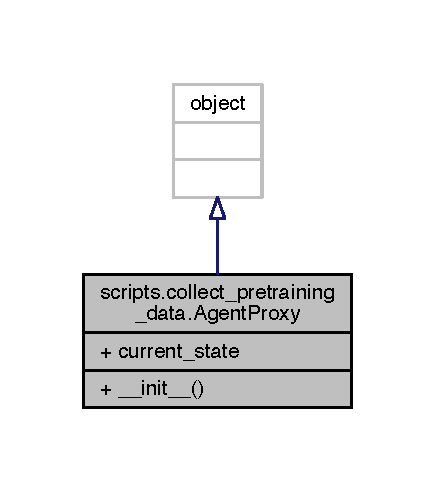
\includegraphics[width=209pt]{classscripts_1_1collect__pretraining__data_1_1_agent_proxy__inherit__graph}
\end{center}
\end{figure}


Collaboration diagram for scripts.\+collect\+\_\+pretraining\+\_\+data.\+Agent\+Proxy\+:\nopagebreak
\begin{figure}[H]
\begin{center}
\leavevmode
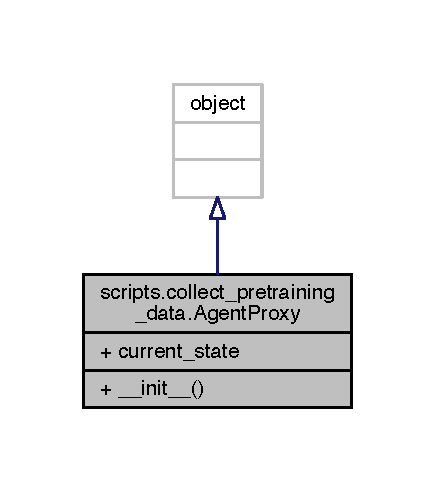
\includegraphics[width=209pt]{classscripts_1_1collect__pretraining__data_1_1_agent_proxy__coll__graph}
\end{center}
\end{figure}
\subsection*{Public Member Functions}
\begin{DoxyCompactItemize}
\item 
\hypertarget{classscripts_1_1collect__pretraining__data_1_1_agent_proxy_af24d25e7cced9bc87e840f6148337f89}{}\label{classscripts_1_1collect__pretraining__data_1_1_agent_proxy_af24d25e7cced9bc87e840f6148337f89} 
def {\bfseries \+\_\+\+\_\+init\+\_\+\+\_\+} (self)
\end{DoxyCompactItemize}
\subsection*{Public Attributes}
\begin{DoxyCompactItemize}
\item 
\hypertarget{classscripts_1_1collect__pretraining__data_1_1_agent_proxy_a5c0b380f09c4cba0dc94b541ca1b8671}{}\label{classscripts_1_1collect__pretraining__data_1_1_agent_proxy_a5c0b380f09c4cba0dc94b541ca1b8671} 
{\bfseries current\+\_\+state}
\end{DoxyCompactItemize}


The documentation for this class was generated from the following file\+:\begin{DoxyCompactItemize}
\item 
aml\+\_\+data\+\_\+collec\+\_\+utils/scripts/collect\+\_\+pretraining\+\_\+data.\+py\end{DoxyCompactItemize}

\hypertarget{classaml__robot_1_1baxter__kinematics_1_1baxter__kinematics}{\section{aml\-\_\-robot.\-baxter\-\_\-kinematics.\-baxter\-\_\-kinematics Class Reference}
\label{classaml__robot_1_1baxter__kinematics_1_1baxter__kinematics}\index{aml\-\_\-robot.\-baxter\-\_\-kinematics.\-baxter\-\_\-kinematics@{aml\-\_\-robot.\-baxter\-\_\-kinematics.\-baxter\-\_\-kinematics}}
}


Inheritance diagram for aml\-\_\-robot.\-baxter\-\_\-kinematics.\-baxter\-\_\-kinematics\-:\nopagebreak
\begin{figure}[H]
\begin{center}
\leavevmode
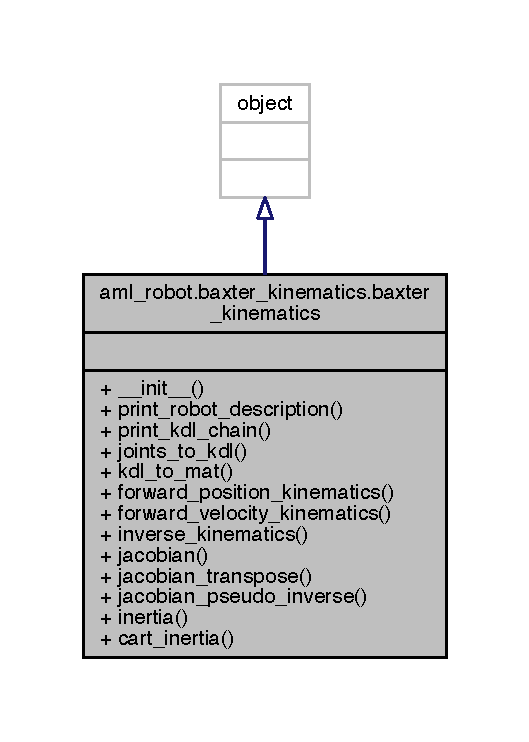
\includegraphics[width=252pt]{classaml__robot_1_1baxter__kinematics_1_1baxter__kinematics__inherit__graph}
\end{center}
\end{figure}


Collaboration diagram for aml\-\_\-robot.\-baxter\-\_\-kinematics.\-baxter\-\_\-kinematics\-:\nopagebreak
\begin{figure}[H]
\begin{center}
\leavevmode
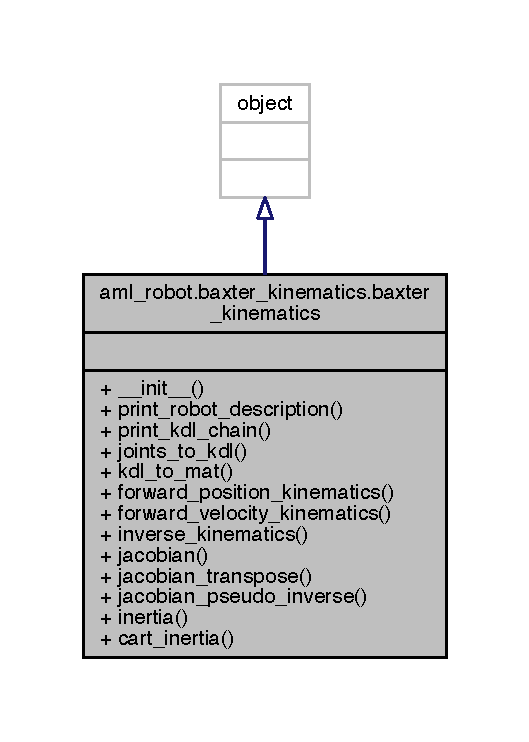
\includegraphics[width=252pt]{classaml__robot_1_1baxter__kinematics_1_1baxter__kinematics__coll__graph}
\end{center}
\end{figure}
\subsection*{Public Member Functions}
\begin{DoxyCompactItemize}
\item 
\hypertarget{classaml__robot_1_1baxter__kinematics_1_1baxter__kinematics_a6a642546348903ad83647e46b3997319}{def {\bfseries \-\_\-\-\_\-init\-\_\-\-\_\-}}\label{classaml__robot_1_1baxter__kinematics_1_1baxter__kinematics_a6a642546348903ad83647e46b3997319}

\item 
\hypertarget{classaml__robot_1_1baxter__kinematics_1_1baxter__kinematics_a5f20f5ed9f8e063544fe0f9269824d77}{def {\bfseries print\-\_\-robot\-\_\-description}}\label{classaml__robot_1_1baxter__kinematics_1_1baxter__kinematics_a5f20f5ed9f8e063544fe0f9269824d77}

\item 
\hypertarget{classaml__robot_1_1baxter__kinematics_1_1baxter__kinematics_a6505980cb91459683b46b4eb0ed5048f}{def {\bfseries print\-\_\-kdl\-\_\-chain}}\label{classaml__robot_1_1baxter__kinematics_1_1baxter__kinematics_a6505980cb91459683b46b4eb0ed5048f}

\item 
\hypertarget{classaml__robot_1_1baxter__kinematics_1_1baxter__kinematics_a5b33fe6f350f58a6b1eab83aa072d847}{def {\bfseries joints\-\_\-to\-\_\-kdl}}\label{classaml__robot_1_1baxter__kinematics_1_1baxter__kinematics_a5b33fe6f350f58a6b1eab83aa072d847}

\item 
\hypertarget{classaml__robot_1_1baxter__kinematics_1_1baxter__kinematics_a4b961c3b58138f41aa1b0f4f34da7e83}{def {\bfseries kdl\-\_\-to\-\_\-mat}}\label{classaml__robot_1_1baxter__kinematics_1_1baxter__kinematics_a4b961c3b58138f41aa1b0f4f34da7e83}

\item 
\hypertarget{classaml__robot_1_1baxter__kinematics_1_1baxter__kinematics_a4c3c9043ae935f5ae5c4bb5806532071}{def {\bfseries forward\-\_\-position\-\_\-kinematics}}\label{classaml__robot_1_1baxter__kinematics_1_1baxter__kinematics_a4c3c9043ae935f5ae5c4bb5806532071}

\item 
\hypertarget{classaml__robot_1_1baxter__kinematics_1_1baxter__kinematics_aca2eef593f0f9e6095c13153401eb948}{def {\bfseries forward\-\_\-velocity\-\_\-kinematics}}\label{classaml__robot_1_1baxter__kinematics_1_1baxter__kinematics_aca2eef593f0f9e6095c13153401eb948}

\item 
\hypertarget{classaml__robot_1_1baxter__kinematics_1_1baxter__kinematics_a5eaca30766683990b213182527cb3813}{def {\bfseries inverse\-\_\-kinematics}}\label{classaml__robot_1_1baxter__kinematics_1_1baxter__kinematics_a5eaca30766683990b213182527cb3813}

\item 
\hypertarget{classaml__robot_1_1baxter__kinematics_1_1baxter__kinematics_a307997661ec9ef26ae4a74bda67a3352}{def {\bfseries jacobian}}\label{classaml__robot_1_1baxter__kinematics_1_1baxter__kinematics_a307997661ec9ef26ae4a74bda67a3352}

\item 
\hypertarget{classaml__robot_1_1baxter__kinematics_1_1baxter__kinematics_a421d5a7383a8b88e7b03efc469f30098}{def {\bfseries jacobian\-\_\-transpose}}\label{classaml__robot_1_1baxter__kinematics_1_1baxter__kinematics_a421d5a7383a8b88e7b03efc469f30098}

\item 
\hypertarget{classaml__robot_1_1baxter__kinematics_1_1baxter__kinematics_ad70f0257064b8a85ee6537e2187822d8}{def {\bfseries jacobian\-\_\-pseudo\-\_\-inverse}}\label{classaml__robot_1_1baxter__kinematics_1_1baxter__kinematics_ad70f0257064b8a85ee6537e2187822d8}

\item 
\hypertarget{classaml__robot_1_1baxter__kinematics_1_1baxter__kinematics_a7fd0653ad6b2012a933822f98901ccce}{def {\bfseries inertia}}\label{classaml__robot_1_1baxter__kinematics_1_1baxter__kinematics_a7fd0653ad6b2012a933822f98901ccce}

\item 
\hypertarget{classaml__robot_1_1baxter__kinematics_1_1baxter__kinematics_af243bf47f45355fb5e71a23ed8b21d28}{def {\bfseries cart\-\_\-inertia}}\label{classaml__robot_1_1baxter__kinematics_1_1baxter__kinematics_af243bf47f45355fb5e71a23ed8b21d28}

\end{DoxyCompactItemize}


\subsection{Detailed Description}
\begin{DoxyVerb}Baxter Kinematics with PyKDL
\end{DoxyVerb}
 

The documentation for this class was generated from the following file\-:\begin{DoxyCompactItemize}
\item 
aml\-\_\-robot/src/aml\-\_\-robot/baxter\-\_\-kinematics.\-py\end{DoxyCompactItemize}

\hypertarget{classaml__robot_1_1baxter__robot_1_1_baxter_arm}{}\section{aml\+\_\+robot.\+baxter\+\_\+robot.\+Baxter\+Arm Class Reference}
\label{classaml__robot_1_1baxter__robot_1_1_baxter_arm}\index{aml\+\_\+robot.\+baxter\+\_\+robot.\+Baxter\+Arm@{aml\+\_\+robot.\+baxter\+\_\+robot.\+Baxter\+Arm}}


Inheritance diagram for aml\+\_\+robot.\+baxter\+\_\+robot.\+Baxter\+Arm\+:
\nopagebreak
\begin{figure}[H]
\begin{center}
\leavevmode
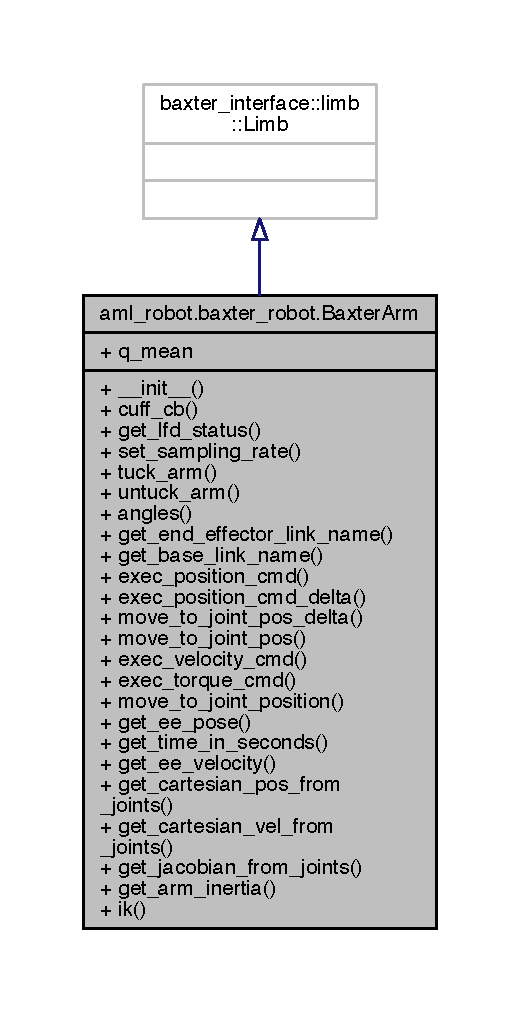
\includegraphics[width=249pt]{classaml__robot_1_1baxter__robot_1_1_baxter_arm__inherit__graph}
\end{center}
\end{figure}


Collaboration diagram for aml\+\_\+robot.\+baxter\+\_\+robot.\+Baxter\+Arm\+:
\nopagebreak
\begin{figure}[H]
\begin{center}
\leavevmode
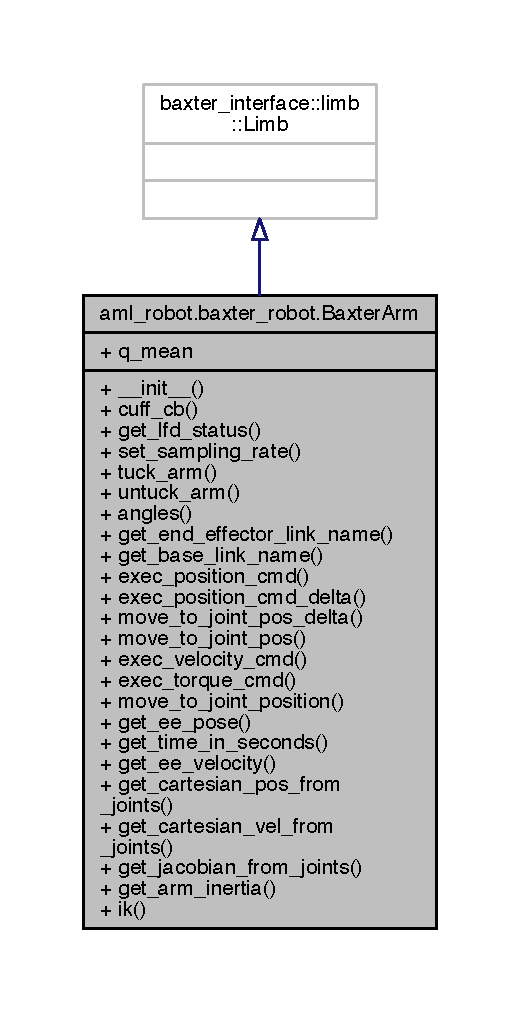
\includegraphics[width=249pt]{classaml__robot_1_1baxter__robot_1_1_baxter_arm__coll__graph}
\end{center}
\end{figure}
\subsection*{Public Member Functions}
\begin{DoxyCompactItemize}
\item 
\hypertarget{classaml__robot_1_1baxter__robot_1_1_baxter_arm_a72a5c161c29bd536c6a8727d3138643a}{}\label{classaml__robot_1_1baxter__robot_1_1_baxter_arm_a72a5c161c29bd536c6a8727d3138643a} 
def {\bfseries \+\_\+\+\_\+init\+\_\+\+\_\+} (self, limb, on\+\_\+state\+\_\+callback=None)
\item 
\hypertarget{classaml__robot_1_1baxter__robot_1_1_baxter_arm_ab8c5985c2c013d2da84e7415f2480f35}{}\label{classaml__robot_1_1baxter__robot_1_1_baxter_arm_ab8c5985c2c013d2da84e7415f2480f35} 
def {\bfseries cuff\+\_\+cb} (self, value)
\item 
\hypertarget{classaml__robot_1_1baxter__robot_1_1_baxter_arm_a08034a334645d8504b391a313add1cc7}{}\label{classaml__robot_1_1baxter__robot_1_1_baxter_arm_a08034a334645d8504b391a313add1cc7} 
def {\bfseries get\+\_\+lfd\+\_\+status} (self)
\item 
\hypertarget{classaml__robot_1_1baxter__robot_1_1_baxter_arm_a1f1b2c10d8e309c0cce60a971f5355b4}{}\label{classaml__robot_1_1baxter__robot_1_1_baxter_arm_a1f1b2c10d8e309c0cce60a971f5355b4} 
def {\bfseries set\+\_\+sampling\+\_\+rate} (self, sampling\+\_\+rate=100)
\item 
\hypertarget{classaml__robot_1_1baxter__robot_1_1_baxter_arm_add8768944b81542e122c676f2b38c075}{}\label{classaml__robot_1_1baxter__robot_1_1_baxter_arm_add8768944b81542e122c676f2b38c075} 
def {\bfseries tuck\+\_\+arm} (self)
\item 
\hypertarget{classaml__robot_1_1baxter__robot_1_1_baxter_arm_af3664aaae25213bf3930c821cbf68432}{}\label{classaml__robot_1_1baxter__robot_1_1_baxter_arm_af3664aaae25213bf3930c821cbf68432} 
def {\bfseries untuck\+\_\+arm} (self)
\item 
\hypertarget{classaml__robot_1_1baxter__robot_1_1_baxter_arm_a0434abfd5899e880a6856444ccc9ecae}{}\label{classaml__robot_1_1baxter__robot_1_1_baxter_arm_a0434abfd5899e880a6856444ccc9ecae} 
def {\bfseries angles} (self)
\item 
\hypertarget{classaml__robot_1_1baxter__robot_1_1_baxter_arm_a40dc93e2269ea57aec71457431984bc0}{}\label{classaml__robot_1_1baxter__robot_1_1_baxter_arm_a40dc93e2269ea57aec71457431984bc0} 
def {\bfseries get\+\_\+end\+\_\+effector\+\_\+link\+\_\+name} (self)
\item 
\hypertarget{classaml__robot_1_1baxter__robot_1_1_baxter_arm_a3d7c1dd8493d6ed1255e856db43e4d9c}{}\label{classaml__robot_1_1baxter__robot_1_1_baxter_arm_a3d7c1dd8493d6ed1255e856db43e4d9c} 
def {\bfseries get\+\_\+base\+\_\+link\+\_\+name} (self)
\item 
\hypertarget{classaml__robot_1_1baxter__robot_1_1_baxter_arm_aa8fb038222939675c5038f546d0e2627}{}\label{classaml__robot_1_1baxter__robot_1_1_baxter_arm_aa8fb038222939675c5038f546d0e2627} 
def {\bfseries exec\+\_\+position\+\_\+cmd} (self, cmd)
\item 
\hypertarget{classaml__robot_1_1baxter__robot_1_1_baxter_arm_a7231f60bcd22ea25ee84d5c3269e82ae}{}\label{classaml__robot_1_1baxter__robot_1_1_baxter_arm_a7231f60bcd22ea25ee84d5c3269e82ae} 
def {\bfseries exec\+\_\+position\+\_\+cmd\+\_\+delta} (self, cmd)
\item 
\hypertarget{classaml__robot_1_1baxter__robot_1_1_baxter_arm_ad4c0f6a22d0cb23f411d50e8f661bcbb}{}\label{classaml__robot_1_1baxter__robot_1_1_baxter_arm_ad4c0f6a22d0cb23f411d50e8f661bcbb} 
def {\bfseries move\+\_\+to\+\_\+joint\+\_\+pos\+\_\+delta} (self, cmd)
\item 
\hypertarget{classaml__robot_1_1baxter__robot_1_1_baxter_arm_a93f87a8500f9e0bfce6be75e41e3ac17}{}\label{classaml__robot_1_1baxter__robot_1_1_baxter_arm_a93f87a8500f9e0bfce6be75e41e3ac17} 
def {\bfseries move\+\_\+to\+\_\+joint\+\_\+pos} (self, cmd)
\item 
\hypertarget{classaml__robot_1_1baxter__robot_1_1_baxter_arm_a3b5cb3d6c651c72bfe9ffd80c867f8f7}{}\label{classaml__robot_1_1baxter__robot_1_1_baxter_arm_a3b5cb3d6c651c72bfe9ffd80c867f8f7} 
def {\bfseries exec\+\_\+velocity\+\_\+cmd} (self, cmd)
\item 
\hypertarget{classaml__robot_1_1baxter__robot_1_1_baxter_arm_aed8c9accc1f637677e4d64583b63d107}{}\label{classaml__robot_1_1baxter__robot_1_1_baxter_arm_aed8c9accc1f637677e4d64583b63d107} 
def {\bfseries exec\+\_\+torque\+\_\+cmd} (self, cmd)
\item 
\hypertarget{classaml__robot_1_1baxter__robot_1_1_baxter_arm_afddcdfa0cafe258cf7f432e7878bc687}{}\label{classaml__robot_1_1baxter__robot_1_1_baxter_arm_afddcdfa0cafe258cf7f432e7878bc687} 
def {\bfseries move\+\_\+to\+\_\+joint\+\_\+position} (self, joint\+\_\+angles)
\item 
\hypertarget{classaml__robot_1_1baxter__robot_1_1_baxter_arm_ac353cdab96098923a40efd30f17f4e7a}{}\label{classaml__robot_1_1baxter__robot_1_1_baxter_arm_ac353cdab96098923a40efd30f17f4e7a} 
def {\bfseries get\+\_\+ee\+\_\+pose} (self)
\item 
\hypertarget{classaml__robot_1_1baxter__robot_1_1_baxter_arm_a9dcc207d5f7703f7f9f69bb54c1ee7b3}{}\label{classaml__robot_1_1baxter__robot_1_1_baxter_arm_a9dcc207d5f7703f7f9f69bb54c1ee7b3} 
def {\bfseries get\+\_\+time\+\_\+in\+\_\+seconds} (self)
\item 
\hypertarget{classaml__robot_1_1baxter__robot_1_1_baxter_arm_a411092f179a7420d38625063c27b237e}{}\label{classaml__robot_1_1baxter__robot_1_1_baxter_arm_a411092f179a7420d38625063c27b237e} 
def {\bfseries get\+\_\+ee\+\_\+velocity} (self, real\+\_\+robot=True)
\item 
\hypertarget{classaml__robot_1_1baxter__robot_1_1_baxter_arm_a9ce9c74c445092b5f9bd26793366c8de}{}\label{classaml__robot_1_1baxter__robot_1_1_baxter_arm_a9ce9c74c445092b5f9bd26793366c8de} 
def {\bfseries get\+\_\+cartesian\+\_\+pos\+\_\+from\+\_\+joints} (self, joint\+\_\+angles=None)
\item 
\hypertarget{classaml__robot_1_1baxter__robot_1_1_baxter_arm_a5d42a91ca13fc1776997909afb999d8f}{}\label{classaml__robot_1_1baxter__robot_1_1_baxter_arm_a5d42a91ca13fc1776997909afb999d8f} 
def {\bfseries get\+\_\+cartesian\+\_\+vel\+\_\+from\+\_\+joints} (self, joint\+\_\+angles=None)
\item 
\hypertarget{classaml__robot_1_1baxter__robot_1_1_baxter_arm_a05c9ee1fe630edbcdc34249bb0c613b3}{}\label{classaml__robot_1_1baxter__robot_1_1_baxter_arm_a05c9ee1fe630edbcdc34249bb0c613b3} 
def {\bfseries get\+\_\+jacobian\+\_\+from\+\_\+joints} (self, joint\+\_\+angles=None)
\item 
\hypertarget{classaml__robot_1_1baxter__robot_1_1_baxter_arm_ae3980ca9408490d07b4460e6d7fc2eb2}{}\label{classaml__robot_1_1baxter__robot_1_1_baxter_arm_ae3980ca9408490d07b4460e6d7fc2eb2} 
def {\bfseries get\+\_\+arm\+\_\+inertia} (self, joint\+\_\+angles=None)
\item 
\hypertarget{classaml__robot_1_1baxter__robot_1_1_baxter_arm_a5ce4a9920b76e223e375755faaef7cf5}{}\label{classaml__robot_1_1baxter__robot_1_1_baxter_arm_a5ce4a9920b76e223e375755faaef7cf5} 
def {\bfseries ik} (self, pos, ori=None)
\end{DoxyCompactItemize}
\subsection*{Public Attributes}
\begin{DoxyCompactItemize}
\item 
\hypertarget{classaml__robot_1_1baxter__robot_1_1_baxter_arm_adf4365cfefdb2632a538a3f225023aa7}{}\label{classaml__robot_1_1baxter__robot_1_1_baxter_arm_adf4365cfefdb2632a538a3f225023aa7} 
{\bfseries q\+\_\+mean}
\end{DoxyCompactItemize}


The documentation for this class was generated from the following file\+:\begin{DoxyCompactItemize}
\item 
aml\+\_\+robot/src/aml\+\_\+robot/baxter\+\_\+robot.\+py\end{DoxyCompactItemize}

\hypertarget{classaml__robot_1_1baxter__robot_1_1_baxter_button_status}{}\section{aml\+\_\+robot.\+baxter\+\_\+robot.\+Baxter\+Button\+Status Class Reference}
\label{classaml__robot_1_1baxter__robot_1_1_baxter_button_status}\index{aml\+\_\+robot.\+baxter\+\_\+robot.\+Baxter\+Button\+Status@{aml\+\_\+robot.\+baxter\+\_\+robot.\+Baxter\+Button\+Status}}


Collaboration diagram for aml\+\_\+robot.\+baxter\+\_\+robot.\+Baxter\+Button\+Status\+:
\nopagebreak
\begin{figure}[H]
\begin{center}
\leavevmode
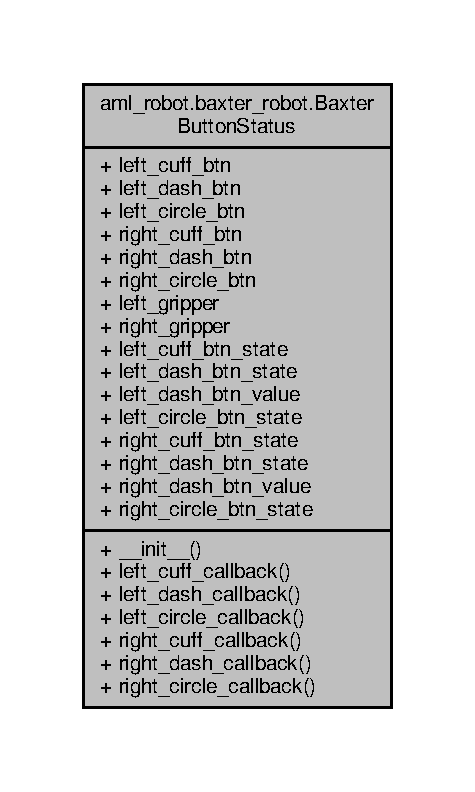
\includegraphics[width=231pt]{classaml__robot_1_1baxter__robot_1_1_baxter_button_status__coll__graph}
\end{center}
\end{figure}
\subsection*{Public Member Functions}
\begin{DoxyCompactItemize}
\item 
\hypertarget{classaml__robot_1_1baxter__robot_1_1_baxter_button_status_a867cbab0efc9f033f193484b7a6ee7d9}{}\label{classaml__robot_1_1baxter__robot_1_1_baxter_button_status_a867cbab0efc9f033f193484b7a6ee7d9} 
def {\bfseries \+\_\+\+\_\+init\+\_\+\+\_\+} (self)
\item 
\hypertarget{classaml__robot_1_1baxter__robot_1_1_baxter_button_status_a0be7e8628a069cee960ba4f84a1fba42}{}\label{classaml__robot_1_1baxter__robot_1_1_baxter_button_status_a0be7e8628a069cee960ba4f84a1fba42} 
def {\bfseries left\+\_\+cuff\+\_\+callback} (self, value)
\item 
\hypertarget{classaml__robot_1_1baxter__robot_1_1_baxter_button_status_a0c7539db9445b453a0eac9e24d402b89}{}\label{classaml__robot_1_1baxter__robot_1_1_baxter_button_status_a0c7539db9445b453a0eac9e24d402b89} 
def {\bfseries left\+\_\+dash\+\_\+callback} (self, value)
\item 
\hypertarget{classaml__robot_1_1baxter__robot_1_1_baxter_button_status_a2a5e12090c441e098b287596bac9b2e9}{}\label{classaml__robot_1_1baxter__robot_1_1_baxter_button_status_a2a5e12090c441e098b287596bac9b2e9} 
def {\bfseries left\+\_\+circle\+\_\+callback} (self, value)
\item 
\hypertarget{classaml__robot_1_1baxter__robot_1_1_baxter_button_status_aea7f6e2c3cb75cc764898bacdf24adad}{}\label{classaml__robot_1_1baxter__robot_1_1_baxter_button_status_aea7f6e2c3cb75cc764898bacdf24adad} 
def {\bfseries right\+\_\+cuff\+\_\+callback} (self, value)
\item 
\hypertarget{classaml__robot_1_1baxter__robot_1_1_baxter_button_status_a9ebd13514e6d978c3a022b99f56d0d2d}{}\label{classaml__robot_1_1baxter__robot_1_1_baxter_button_status_a9ebd13514e6d978c3a022b99f56d0d2d} 
def {\bfseries right\+\_\+dash\+\_\+callback} (self, value)
\item 
\hypertarget{classaml__robot_1_1baxter__robot_1_1_baxter_button_status_a80e8aebd2bf7ceb32d63bade6e078eff}{}\label{classaml__robot_1_1baxter__robot_1_1_baxter_button_status_a80e8aebd2bf7ceb32d63bade6e078eff} 
def {\bfseries right\+\_\+circle\+\_\+callback} (self, value)
\end{DoxyCompactItemize}
\subsection*{Public Attributes}
\begin{DoxyCompactItemize}
\item 
\hypertarget{classaml__robot_1_1baxter__robot_1_1_baxter_button_status_a04619f9d86af362ba45b652a30f75186}{}\label{classaml__robot_1_1baxter__robot_1_1_baxter_button_status_a04619f9d86af362ba45b652a30f75186} 
{\bfseries left\+\_\+cuff\+\_\+btn}
\item 
\hypertarget{classaml__robot_1_1baxter__robot_1_1_baxter_button_status_a8bf46c388908af610775a7853f12db6b}{}\label{classaml__robot_1_1baxter__robot_1_1_baxter_button_status_a8bf46c388908af610775a7853f12db6b} 
{\bfseries left\+\_\+dash\+\_\+btn}
\item 
\hypertarget{classaml__robot_1_1baxter__robot_1_1_baxter_button_status_aafc55b8a39cd12b8b916c1f9e4e101cb}{}\label{classaml__robot_1_1baxter__robot_1_1_baxter_button_status_aafc55b8a39cd12b8b916c1f9e4e101cb} 
{\bfseries left\+\_\+circle\+\_\+btn}
\item 
\hypertarget{classaml__robot_1_1baxter__robot_1_1_baxter_button_status_a96d1d159449f8937e2c8605ffb359e26}{}\label{classaml__robot_1_1baxter__robot_1_1_baxter_button_status_a96d1d159449f8937e2c8605ffb359e26} 
{\bfseries right\+\_\+cuff\+\_\+btn}
\item 
\hypertarget{classaml__robot_1_1baxter__robot_1_1_baxter_button_status_a20e886d155229257692984a1fc790216}{}\label{classaml__robot_1_1baxter__robot_1_1_baxter_button_status_a20e886d155229257692984a1fc790216} 
{\bfseries right\+\_\+dash\+\_\+btn}
\item 
\hypertarget{classaml__robot_1_1baxter__robot_1_1_baxter_button_status_af554ad16b5a28ab857cdc6c1d0e92ad8}{}\label{classaml__robot_1_1baxter__robot_1_1_baxter_button_status_af554ad16b5a28ab857cdc6c1d0e92ad8} 
{\bfseries right\+\_\+circle\+\_\+btn}
\item 
\hypertarget{classaml__robot_1_1baxter__robot_1_1_baxter_button_status_a1c2a8b264d928929fa9cad5d97bdc817}{}\label{classaml__robot_1_1baxter__robot_1_1_baxter_button_status_a1c2a8b264d928929fa9cad5d97bdc817} 
{\bfseries left\+\_\+gripper}
\item 
\hypertarget{classaml__robot_1_1baxter__robot_1_1_baxter_button_status_a1dd2e91ddd93d9c40dc8e7f83926d908}{}\label{classaml__robot_1_1baxter__robot_1_1_baxter_button_status_a1dd2e91ddd93d9c40dc8e7f83926d908} 
{\bfseries right\+\_\+gripper}
\item 
\hypertarget{classaml__robot_1_1baxter__robot_1_1_baxter_button_status_a3d147c0e2ab38474d2cb2d2cb358e9c6}{}\label{classaml__robot_1_1baxter__robot_1_1_baxter_button_status_a3d147c0e2ab38474d2cb2d2cb358e9c6} 
{\bfseries left\+\_\+cuff\+\_\+btn\+\_\+state}
\item 
\hypertarget{classaml__robot_1_1baxter__robot_1_1_baxter_button_status_a9858defbdfd1953111bc032a679dfbf6}{}\label{classaml__robot_1_1baxter__robot_1_1_baxter_button_status_a9858defbdfd1953111bc032a679dfbf6} 
{\bfseries left\+\_\+dash\+\_\+btn\+\_\+state}
\item 
\hypertarget{classaml__robot_1_1baxter__robot_1_1_baxter_button_status_ac4505635cb0c3096d50145a00aa996e1}{}\label{classaml__robot_1_1baxter__robot_1_1_baxter_button_status_ac4505635cb0c3096d50145a00aa996e1} 
{\bfseries left\+\_\+dash\+\_\+btn\+\_\+value}
\item 
\hypertarget{classaml__robot_1_1baxter__robot_1_1_baxter_button_status_a2cf8425649007e50335a7eab640138bd}{}\label{classaml__robot_1_1baxter__robot_1_1_baxter_button_status_a2cf8425649007e50335a7eab640138bd} 
{\bfseries left\+\_\+circle\+\_\+btn\+\_\+state}
\item 
\hypertarget{classaml__robot_1_1baxter__robot_1_1_baxter_button_status_a0b2de8e8474d9e9217024692b425a0b4}{}\label{classaml__robot_1_1baxter__robot_1_1_baxter_button_status_a0b2de8e8474d9e9217024692b425a0b4} 
{\bfseries right\+\_\+cuff\+\_\+btn\+\_\+state}
\item 
\hypertarget{classaml__robot_1_1baxter__robot_1_1_baxter_button_status_a99abdcffd19c44a10cb1f4a875adbb2d}{}\label{classaml__robot_1_1baxter__robot_1_1_baxter_button_status_a99abdcffd19c44a10cb1f4a875adbb2d} 
{\bfseries right\+\_\+dash\+\_\+btn\+\_\+state}
\item 
\hypertarget{classaml__robot_1_1baxter__robot_1_1_baxter_button_status_a990924b4c4d0b7f05b7fc909b3b7cc2f}{}\label{classaml__robot_1_1baxter__robot_1_1_baxter_button_status_a990924b4c4d0b7f05b7fc909b3b7cc2f} 
{\bfseries right\+\_\+dash\+\_\+btn\+\_\+value}
\item 
\hypertarget{classaml__robot_1_1baxter__robot_1_1_baxter_button_status_a6b266aa0af869f160bd2654e6fde6756}{}\label{classaml__robot_1_1baxter__robot_1_1_baxter_button_status_a6b266aa0af869f160bd2654e6fde6756} 
{\bfseries right\+\_\+circle\+\_\+btn\+\_\+state}
\end{DoxyCompactItemize}


The documentation for this class was generated from the following file\+:\begin{DoxyCompactItemize}
\item 
aml\+\_\+robot/src/aml\+\_\+robot/baxter\+\_\+robot.\+py\end{DoxyCompactItemize}

\hypertarget{classscripts_1_1camera__calib_1_1_baxter_eye_hand_calib}{\section{scripts.\-camera\-\_\-calib.\-Baxter\-Eye\-Hand\-Calib Class Reference}
\label{classscripts_1_1camera__calib_1_1_baxter_eye_hand_calib}\index{scripts.\-camera\-\_\-calib.\-Baxter\-Eye\-Hand\-Calib@{scripts.\-camera\-\_\-calib.\-Baxter\-Eye\-Hand\-Calib}}
}


Collaboration diagram for scripts.\-camera\-\_\-calib.\-Baxter\-Eye\-Hand\-Calib\-:\nopagebreak
\begin{figure}[H]
\begin{center}
\leavevmode
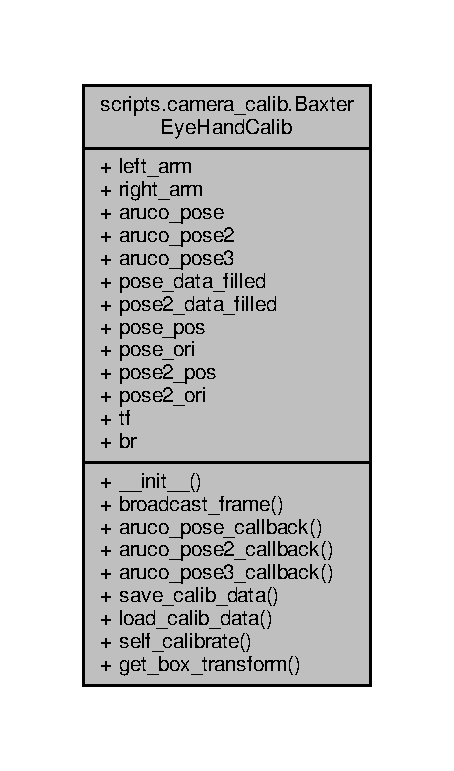
\includegraphics[width=218pt]{classscripts_1_1camera__calib_1_1_baxter_eye_hand_calib__coll__graph}
\end{center}
\end{figure}
\subsection*{Public Member Functions}
\begin{DoxyCompactItemize}
\item 
\hypertarget{classscripts_1_1camera__calib_1_1_baxter_eye_hand_calib_a80e6fdbd3328978e83856bc1f9511904}{def {\bfseries \-\_\-\-\_\-init\-\_\-\-\_\-}}\label{classscripts_1_1camera__calib_1_1_baxter_eye_hand_calib_a80e6fdbd3328978e83856bc1f9511904}

\item 
\hypertarget{classscripts_1_1camera__calib_1_1_baxter_eye_hand_calib_a5e488e63f6aba8960984276bf46df832}{def {\bfseries broadcast\-\_\-frame}}\label{classscripts_1_1camera__calib_1_1_baxter_eye_hand_calib_a5e488e63f6aba8960984276bf46df832}

\item 
\hypertarget{classscripts_1_1camera__calib_1_1_baxter_eye_hand_calib_ab26f80c1371115eda5b2b577597418c8}{def {\bfseries aruco\-\_\-pose\-\_\-callback}}\label{classscripts_1_1camera__calib_1_1_baxter_eye_hand_calib_ab26f80c1371115eda5b2b577597418c8}

\item 
\hypertarget{classscripts_1_1camera__calib_1_1_baxter_eye_hand_calib_a9e60a5b9a52220778599138f43da54c8}{def {\bfseries aruco\-\_\-pose2\-\_\-callback}}\label{classscripts_1_1camera__calib_1_1_baxter_eye_hand_calib_a9e60a5b9a52220778599138f43da54c8}

\item 
\hypertarget{classscripts_1_1camera__calib_1_1_baxter_eye_hand_calib_a9c9358fd48969228d5c8ffc2bc055b04}{def {\bfseries aruco\-\_\-pose3\-\_\-callback}}\label{classscripts_1_1camera__calib_1_1_baxter_eye_hand_calib_a9c9358fd48969228d5c8ffc2bc055b04}

\item 
\hypertarget{classscripts_1_1camera__calib_1_1_baxter_eye_hand_calib_a2b90ecd8fd8ee5cb210e868b2a90997a}{def {\bfseries save\-\_\-calib\-\_\-data}}\label{classscripts_1_1camera__calib_1_1_baxter_eye_hand_calib_a2b90ecd8fd8ee5cb210e868b2a90997a}

\item 
\hypertarget{classscripts_1_1camera__calib_1_1_baxter_eye_hand_calib_aca74cf091daafb370191e195e95b62e6}{def {\bfseries load\-\_\-calib\-\_\-data}}\label{classscripts_1_1camera__calib_1_1_baxter_eye_hand_calib_aca74cf091daafb370191e195e95b62e6}

\item 
\hypertarget{classscripts_1_1camera__calib_1_1_baxter_eye_hand_calib_ad46242daa5c68b20fd1d460c2542d761}{def {\bfseries self\-\_\-calibrate}}\label{classscripts_1_1camera__calib_1_1_baxter_eye_hand_calib_ad46242daa5c68b20fd1d460c2542d761}

\item 
\hypertarget{classscripts_1_1camera__calib_1_1_baxter_eye_hand_calib_abd71ea660f2e0b548c2606cd20f404a4}{def {\bfseries get\-\_\-box\-\_\-transform}}\label{classscripts_1_1camera__calib_1_1_baxter_eye_hand_calib_abd71ea660f2e0b548c2606cd20f404a4}

\end{DoxyCompactItemize}
\subsection*{Public Attributes}
\begin{DoxyCompactItemize}
\item 
\hypertarget{classscripts_1_1camera__calib_1_1_baxter_eye_hand_calib_ad56b37f9835ab1d410a14321d0ccdc7d}{{\bfseries left\-\_\-arm}}\label{classscripts_1_1camera__calib_1_1_baxter_eye_hand_calib_ad56b37f9835ab1d410a14321d0ccdc7d}

\item 
\hypertarget{classscripts_1_1camera__calib_1_1_baxter_eye_hand_calib_a1e8eb78f3692768af3b48ed999bc9cc9}{{\bfseries right\-\_\-arm}}\label{classscripts_1_1camera__calib_1_1_baxter_eye_hand_calib_a1e8eb78f3692768af3b48ed999bc9cc9}

\item 
\hypertarget{classscripts_1_1camera__calib_1_1_baxter_eye_hand_calib_ad568784ea9ac30513293bba1aea2a857}{{\bfseries aruco\-\_\-pose}}\label{classscripts_1_1camera__calib_1_1_baxter_eye_hand_calib_ad568784ea9ac30513293bba1aea2a857}

\item 
\hypertarget{classscripts_1_1camera__calib_1_1_baxter_eye_hand_calib_a286f3e64b708fa5e421081a541112c9b}{{\bfseries aruco\-\_\-pose2}}\label{classscripts_1_1camera__calib_1_1_baxter_eye_hand_calib_a286f3e64b708fa5e421081a541112c9b}

\item 
\hypertarget{classscripts_1_1camera__calib_1_1_baxter_eye_hand_calib_a9b482e44d1f456a7212caf8b04a82623}{{\bfseries aruco\-\_\-pose3}}\label{classscripts_1_1camera__calib_1_1_baxter_eye_hand_calib_a9b482e44d1f456a7212caf8b04a82623}

\item 
\hypertarget{classscripts_1_1camera__calib_1_1_baxter_eye_hand_calib_a4a485c29284a2921e762d4599c736bd1}{{\bfseries pose\-\_\-data\-\_\-filled}}\label{classscripts_1_1camera__calib_1_1_baxter_eye_hand_calib_a4a485c29284a2921e762d4599c736bd1}

\item 
\hypertarget{classscripts_1_1camera__calib_1_1_baxter_eye_hand_calib_ad87ce37e7087b0c8a5219821b4712e27}{{\bfseries pose2\-\_\-data\-\_\-filled}}\label{classscripts_1_1camera__calib_1_1_baxter_eye_hand_calib_ad87ce37e7087b0c8a5219821b4712e27}

\item 
\hypertarget{classscripts_1_1camera__calib_1_1_baxter_eye_hand_calib_ad98e6855ab85a0ddc846282de39cc74f}{{\bfseries pose\-\_\-pos}}\label{classscripts_1_1camera__calib_1_1_baxter_eye_hand_calib_ad98e6855ab85a0ddc846282de39cc74f}

\item 
\hypertarget{classscripts_1_1camera__calib_1_1_baxter_eye_hand_calib_afeed0b6826a0e6dd3362fa84138c06cf}{{\bfseries pose\-\_\-ori}}\label{classscripts_1_1camera__calib_1_1_baxter_eye_hand_calib_afeed0b6826a0e6dd3362fa84138c06cf}

\item 
\hypertarget{classscripts_1_1camera__calib_1_1_baxter_eye_hand_calib_adcb4f9d2feb400ef7ca8bb0672d23ea2}{{\bfseries pose2\-\_\-pos}}\label{classscripts_1_1camera__calib_1_1_baxter_eye_hand_calib_adcb4f9d2feb400ef7ca8bb0672d23ea2}

\item 
\hypertarget{classscripts_1_1camera__calib_1_1_baxter_eye_hand_calib_accdcaa8aa525885e280f8618040a0927}{{\bfseries pose2\-\_\-ori}}\label{classscripts_1_1camera__calib_1_1_baxter_eye_hand_calib_accdcaa8aa525885e280f8618040a0927}

\item 
\hypertarget{classscripts_1_1camera__calib_1_1_baxter_eye_hand_calib_a8c775943efd1fb7730e739366b295027}{{\bfseries tf}}\label{classscripts_1_1camera__calib_1_1_baxter_eye_hand_calib_a8c775943efd1fb7730e739366b295027}

\item 
\hypertarget{classscripts_1_1camera__calib_1_1_baxter_eye_hand_calib_a9d083d71d6425de359b3550c16fc97a6}{{\bfseries br}}\label{classscripts_1_1camera__calib_1_1_baxter_eye_hand_calib_a9d083d71d6425de359b3550c16fc97a6}

\end{DoxyCompactItemize}


The documentation for this class was generated from the following file\-:\begin{DoxyCompactItemize}
\item 
aml\-\_\-calib/scripts/camera\-\_\-calib.\-py\end{DoxyCompactItemize}

\hypertarget{classaml__ctrl_1_1controllers_1_1os__controllers_1_1os__moveit__baxter__controller_1_1_baxter_move_it_controller}{}\section{aml\+\_\+ctrl.\+controllers.\+os\+\_\+controllers.\+os\+\_\+moveit\+\_\+baxter\+\_\+controller.\+Baxter\+Move\+It\+Controller Class Reference}
\label{classaml__ctrl_1_1controllers_1_1os__controllers_1_1os__moveit__baxter__controller_1_1_baxter_move_it_controller}\index{aml\+\_\+ctrl.\+controllers.\+os\+\_\+controllers.\+os\+\_\+moveit\+\_\+baxter\+\_\+controller.\+Baxter\+Move\+It\+Controller@{aml\+\_\+ctrl.\+controllers.\+os\+\_\+controllers.\+os\+\_\+moveit\+\_\+baxter\+\_\+controller.\+Baxter\+Move\+It\+Controller}}


Collaboration diagram for aml\+\_\+ctrl.\+controllers.\+os\+\_\+controllers.\+os\+\_\+moveit\+\_\+baxter\+\_\+controller.\+Baxter\+Move\+It\+Controller\+:\nopagebreak
\begin{figure}[H]
\begin{center}
\leavevmode
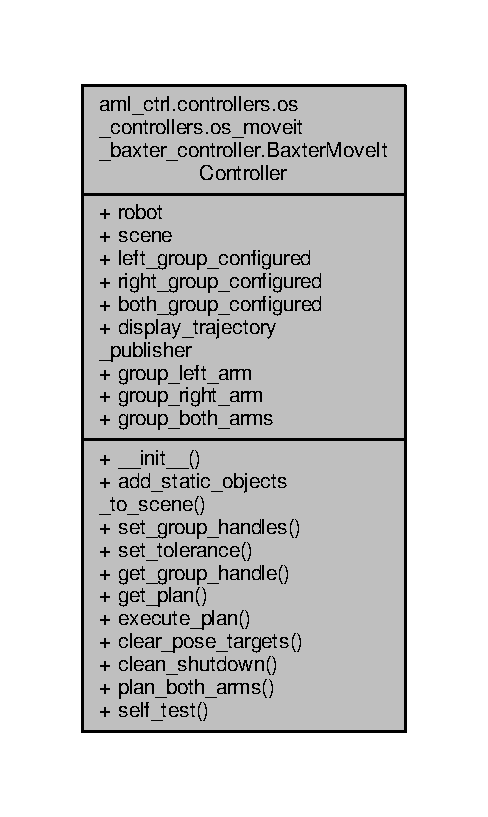
\includegraphics[width=237pt]{classaml__ctrl_1_1controllers_1_1os__controllers_1_1os__moveit__baxter__controller_1_1_baxter_move_it_controller__coll__graph}
\end{center}
\end{figure}
\subsection*{Public Member Functions}
\begin{DoxyCompactItemize}
\item 
\hypertarget{classaml__ctrl_1_1controllers_1_1os__controllers_1_1os__moveit__baxter__controller_1_1_baxter_move_it_controller_a1a84873529afbe9a69e6417b081c69b6}{}\label{classaml__ctrl_1_1controllers_1_1os__controllers_1_1os__moveit__baxter__controller_1_1_baxter_move_it_controller_a1a84873529afbe9a69e6417b081c69b6} 
def {\bfseries \+\_\+\+\_\+init\+\_\+\+\_\+} (self)
\item 
\hypertarget{classaml__ctrl_1_1controllers_1_1os__controllers_1_1os__moveit__baxter__controller_1_1_baxter_move_it_controller_aee42fd2df699bf36bacab48c62a3f835}{}\label{classaml__ctrl_1_1controllers_1_1os__controllers_1_1os__moveit__baxter__controller_1_1_baxter_move_it_controller_aee42fd2df699bf36bacab48c62a3f835} 
def {\bfseries add\+\_\+static\+\_\+objects\+\_\+to\+\_\+scene} (self, limb\+\_\+group=0, obj\+\_\+pos=None, obj\+\_\+ori=None)
\item 
\hypertarget{classaml__ctrl_1_1controllers_1_1os__controllers_1_1os__moveit__baxter__controller_1_1_baxter_move_it_controller_a8654d7c265d7b24cd100f9d48b27009e}{}\label{classaml__ctrl_1_1controllers_1_1os__controllers_1_1os__moveit__baxter__controller_1_1_baxter_move_it_controller_a8654d7c265d7b24cd100f9d48b27009e} 
def {\bfseries set\+\_\+group\+\_\+handles} (self, limb\+\_\+group=1)
\item 
\hypertarget{classaml__ctrl_1_1controllers_1_1os__controllers_1_1os__moveit__baxter__controller_1_1_baxter_move_it_controller_a5c36ba80284c58cd330250fe22df2b5f}{}\label{classaml__ctrl_1_1controllers_1_1os__controllers_1_1os__moveit__baxter__controller_1_1_baxter_move_it_controller_a5c36ba80284c58cd330250fe22df2b5f} 
def {\bfseries set\+\_\+tolerance} (self, group\+\_\+handle, pos\+\_\+tol=0.\+01, ori\+\_\+tol=0.\+01)
\item 
\hypertarget{classaml__ctrl_1_1controllers_1_1os__controllers_1_1os__moveit__baxter__controller_1_1_baxter_move_it_controller_a64def61cb6183744bb7811b12ae44f9d}{}\label{classaml__ctrl_1_1controllers_1_1os__controllers_1_1os__moveit__baxter__controller_1_1_baxter_move_it_controller_a64def61cb6183744bb7811b12ae44f9d} 
def {\bfseries get\+\_\+group\+\_\+handle} (self, limb\+\_\+group=1)
\item 
\hypertarget{classaml__ctrl_1_1controllers_1_1os__controllers_1_1os__moveit__baxter__controller_1_1_baxter_move_it_controller_a7a3f0ed80f28cc25fde582192593294e}{}\label{classaml__ctrl_1_1controllers_1_1os__controllers_1_1os__moveit__baxter__controller_1_1_baxter_move_it_controller_a7a3f0ed80f28cc25fde582192593294e} 
def {\bfseries get\+\_\+plan} (self, limb\+\_\+group, pos, ori, wait\+\_\+time=1.\+5)
\item 
\hypertarget{classaml__ctrl_1_1controllers_1_1os__controllers_1_1os__moveit__baxter__controller_1_1_baxter_move_it_controller_a2b49e5087fb6eaa70c6d13b768fdd164}{}\label{classaml__ctrl_1_1controllers_1_1os__controllers_1_1os__moveit__baxter__controller_1_1_baxter_move_it_controller_a2b49e5087fb6eaa70c6d13b768fdd164} 
def {\bfseries execute\+\_\+plan} (self, limb\+\_\+group, plan, real\+\_\+robot=False)
\item 
\hypertarget{classaml__ctrl_1_1controllers_1_1os__controllers_1_1os__moveit__baxter__controller_1_1_baxter_move_it_controller_ad5a033cc3fe8ed279770142466382764}{}\label{classaml__ctrl_1_1controllers_1_1os__controllers_1_1os__moveit__baxter__controller_1_1_baxter_move_it_controller_ad5a033cc3fe8ed279770142466382764} 
def {\bfseries clear\+\_\+pose\+\_\+targets} (self, limb\+\_\+group=1)
\item 
\hypertarget{classaml__ctrl_1_1controllers_1_1os__controllers_1_1os__moveit__baxter__controller_1_1_baxter_move_it_controller_a775b3416eb7d00d6270e69df81fd9e49}{}\label{classaml__ctrl_1_1controllers_1_1os__controllers_1_1os__moveit__baxter__controller_1_1_baxter_move_it_controller_a775b3416eb7d00d6270e69df81fd9e49} 
def {\bfseries clean\+\_\+shutdown} (self)
\item 
\hypertarget{classaml__ctrl_1_1controllers_1_1os__controllers_1_1os__moveit__baxter__controller_1_1_baxter_move_it_controller_a862572cd81154f514ea5044bf8cd7773}{}\label{classaml__ctrl_1_1controllers_1_1os__controllers_1_1os__moveit__baxter__controller_1_1_baxter_move_it_controller_a862572cd81154f514ea5044bf8cd7773} 
def {\bfseries plan\+\_\+both\+\_\+arms} (self, left\+\_\+pos, left\+\_\+ori, right\+\_\+pos, right\+\_\+ori)
\item 
\hypertarget{classaml__ctrl_1_1controllers_1_1os__controllers_1_1os__moveit__baxter__controller_1_1_baxter_move_it_controller_a76cb945e9e88f0d902e820cf1d1421c4}{}\label{classaml__ctrl_1_1controllers_1_1os__controllers_1_1os__moveit__baxter__controller_1_1_baxter_move_it_controller_a76cb945e9e88f0d902e820cf1d1421c4} 
def {\bfseries self\+\_\+test} (self, limb\+\_\+group=1)
\end{DoxyCompactItemize}
\subsection*{Public Attributes}
\begin{DoxyCompactItemize}
\item 
\hypertarget{classaml__ctrl_1_1controllers_1_1os__controllers_1_1os__moveit__baxter__controller_1_1_baxter_move_it_controller_a1c534361d1c6f82e6e6d0781097410bc}{}\label{classaml__ctrl_1_1controllers_1_1os__controllers_1_1os__moveit__baxter__controller_1_1_baxter_move_it_controller_a1c534361d1c6f82e6e6d0781097410bc} 
{\bfseries robot}
\item 
\hypertarget{classaml__ctrl_1_1controllers_1_1os__controllers_1_1os__moveit__baxter__controller_1_1_baxter_move_it_controller_abde30d477cfd2f39c9a7fe6e1227028b}{}\label{classaml__ctrl_1_1controllers_1_1os__controllers_1_1os__moveit__baxter__controller_1_1_baxter_move_it_controller_abde30d477cfd2f39c9a7fe6e1227028b} 
{\bfseries scene}
\item 
\hypertarget{classaml__ctrl_1_1controllers_1_1os__controllers_1_1os__moveit__baxter__controller_1_1_baxter_move_it_controller_a44ac924f2a51afd683e775fe6dc7baca}{}\label{classaml__ctrl_1_1controllers_1_1os__controllers_1_1os__moveit__baxter__controller_1_1_baxter_move_it_controller_a44ac924f2a51afd683e775fe6dc7baca} 
{\bfseries left\+\_\+group\+\_\+configured}
\item 
\hypertarget{classaml__ctrl_1_1controllers_1_1os__controllers_1_1os__moveit__baxter__controller_1_1_baxter_move_it_controller_a12e7944ade73dc34e96e1bef3949ae58}{}\label{classaml__ctrl_1_1controllers_1_1os__controllers_1_1os__moveit__baxter__controller_1_1_baxter_move_it_controller_a12e7944ade73dc34e96e1bef3949ae58} 
{\bfseries right\+\_\+group\+\_\+configured}
\item 
\hypertarget{classaml__ctrl_1_1controllers_1_1os__controllers_1_1os__moveit__baxter__controller_1_1_baxter_move_it_controller_aa9c8571105d028ff6e64a7cee0d10393}{}\label{classaml__ctrl_1_1controllers_1_1os__controllers_1_1os__moveit__baxter__controller_1_1_baxter_move_it_controller_aa9c8571105d028ff6e64a7cee0d10393} 
{\bfseries both\+\_\+group\+\_\+configured}
\item 
\hypertarget{classaml__ctrl_1_1controllers_1_1os__controllers_1_1os__moveit__baxter__controller_1_1_baxter_move_it_controller_ae424f29d48a9139e177314a1ec9735e3}{}\label{classaml__ctrl_1_1controllers_1_1os__controllers_1_1os__moveit__baxter__controller_1_1_baxter_move_it_controller_ae424f29d48a9139e177314a1ec9735e3} 
{\bfseries display\+\_\+trajectory\+\_\+publisher}
\item 
\hypertarget{classaml__ctrl_1_1controllers_1_1os__controllers_1_1os__moveit__baxter__controller_1_1_baxter_move_it_controller_a6750fdc448f782cfbd3bf1859c8e2503}{}\label{classaml__ctrl_1_1controllers_1_1os__controllers_1_1os__moveit__baxter__controller_1_1_baxter_move_it_controller_a6750fdc448f782cfbd3bf1859c8e2503} 
{\bfseries group\+\_\+left\+\_\+arm}
\item 
\hypertarget{classaml__ctrl_1_1controllers_1_1os__controllers_1_1os__moveit__baxter__controller_1_1_baxter_move_it_controller_afbc743ae405edc5f8974c7b89732aaa7}{}\label{classaml__ctrl_1_1controllers_1_1os__controllers_1_1os__moveit__baxter__controller_1_1_baxter_move_it_controller_afbc743ae405edc5f8974c7b89732aaa7} 
{\bfseries group\+\_\+right\+\_\+arm}
\item 
\hypertarget{classaml__ctrl_1_1controllers_1_1os__controllers_1_1os__moveit__baxter__controller_1_1_baxter_move_it_controller_a8fa5f00622d9497afe8d8df91a0bbe9f}{}\label{classaml__ctrl_1_1controllers_1_1os__controllers_1_1os__moveit__baxter__controller_1_1_baxter_move_it_controller_a8fa5f00622d9497afe8d8df91a0bbe9f} 
{\bfseries group\+\_\+both\+\_\+arms}
\end{DoxyCompactItemize}


The documentation for this class was generated from the following file\+:\begin{DoxyCompactItemize}
\item 
aml\+\_\+ctrl/src/aml\+\_\+ctrl/controllers/os\+\_\+controllers/os\+\_\+moveit\+\_\+baxter\+\_\+controller.\+py\end{DoxyCompactItemize}

\hypertarget{classscripts_1_1collect__push__data_1_1_box_object}{}\section{scripts.\+collect\+\_\+push\+\_\+data.\+Box\+Object Class Reference}
\label{classscripts_1_1collect__push__data_1_1_box_object}\index{scripts.\+collect\+\_\+push\+\_\+data.\+Box\+Object@{scripts.\+collect\+\_\+push\+\_\+data.\+Box\+Object}}


Inheritance diagram for scripts.\+collect\+\_\+push\+\_\+data.\+Box\+Object\+:\nopagebreak
\begin{figure}[H]
\begin{center}
\leavevmode
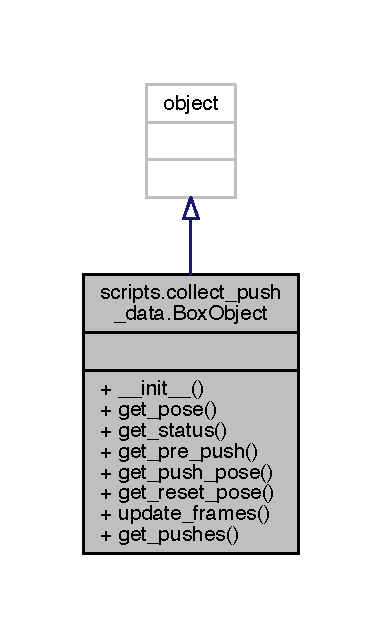
\includegraphics[width=183pt]{classscripts_1_1collect__push__data_1_1_box_object__inherit__graph}
\end{center}
\end{figure}


Collaboration diagram for scripts.\+collect\+\_\+push\+\_\+data.\+Box\+Object\+:\nopagebreak
\begin{figure}[H]
\begin{center}
\leavevmode
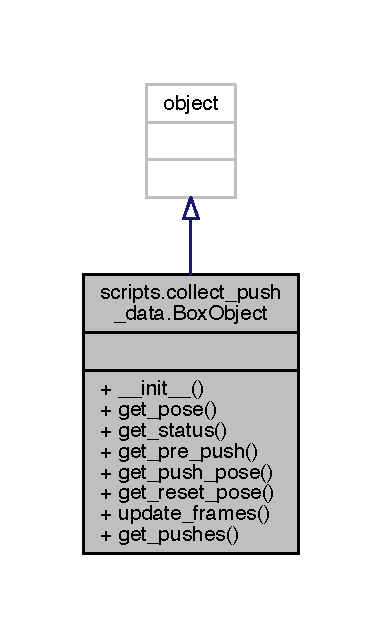
\includegraphics[width=183pt]{classscripts_1_1collect__push__data_1_1_box_object__coll__graph}
\end{center}
\end{figure}
\subsection*{Public Member Functions}
\begin{DoxyCompactItemize}
\item 
\hypertarget{classscripts_1_1collect__push__data_1_1_box_object_ad68ce2001ed164296e78e7dc82f64d0c}{}\label{classscripts_1_1collect__push__data_1_1_box_object_ad68ce2001ed164296e78e7dc82f64d0c} 
def {\bfseries \+\_\+\+\_\+init\+\_\+\+\_\+} (self)
\item 
\hypertarget{classscripts_1_1collect__push__data_1_1_box_object_adbdf92548b76002c379f5b60bb9595b2}{}\label{classscripts_1_1collect__push__data_1_1_box_object_adbdf92548b76002c379f5b60bb9595b2} 
def {\bfseries get\+\_\+pose} (self)
\item 
\hypertarget{classscripts_1_1collect__push__data_1_1_box_object_a8805e17b45fc416036ed7ee43cc30820}{}\label{classscripts_1_1collect__push__data_1_1_box_object_a8805e17b45fc416036ed7ee43cc30820} 
def {\bfseries get\+\_\+status} (self)
\item 
\hypertarget{classscripts_1_1collect__push__data_1_1_box_object_a9b9c05857b70c0625004f21fcc3257fe}{}\label{classscripts_1_1collect__push__data_1_1_box_object_a9b9c05857b70c0625004f21fcc3257fe} 
def {\bfseries get\+\_\+pre\+\_\+push} (self, idx)
\item 
\hypertarget{classscripts_1_1collect__push__data_1_1_box_object_aef4c40b8c89122ed6572ad767a7b9b31}{}\label{classscripts_1_1collect__push__data_1_1_box_object_aef4c40b8c89122ed6572ad767a7b9b31} 
def {\bfseries get\+\_\+push\+\_\+pose} (self)
\item 
\hypertarget{classscripts_1_1collect__push__data_1_1_box_object_a585974b669fefb8fa2b096303238d920}{}\label{classscripts_1_1collect__push__data_1_1_box_object_a585974b669fefb8fa2b096303238d920} 
def {\bfseries get\+\_\+reset\+\_\+pose} (self)
\item 
\hypertarget{classscripts_1_1collect__push__data_1_1_box_object_a44880e249d6ba7435251c990e812f953}{}\label{classscripts_1_1collect__push__data_1_1_box_object_a44880e249d6ba7435251c990e812f953} 
def {\bfseries update\+\_\+frames} (self, event)
\item 
\hypertarget{classscripts_1_1collect__push__data_1_1_box_object_ad766b16187bc3fb74d748493d83640e7}{}\label{classscripts_1_1collect__push__data_1_1_box_object_ad766b16187bc3fb74d748493d83640e7} 
def {\bfseries get\+\_\+pushes} (self)
\end{DoxyCompactItemize}


The documentation for this class was generated from the following file\+:\begin{DoxyCompactItemize}
\item 
aml\+\_\+data\+\_\+collec\+\_\+utils/scripts/collect\+\_\+push\+\_\+data.\+py\end{DoxyCompactItemize}

\hypertarget{classaml__perception_1_1camera__sensor_1_1_camera_sensor}{\section{aml\-\_\-perception.\-camera\-\_\-sensor.\-Camera\-Sensor Class Reference}
\label{classaml__perception_1_1camera__sensor_1_1_camera_sensor}\index{aml\-\_\-perception.\-camera\-\_\-sensor.\-Camera\-Sensor@{aml\-\_\-perception.\-camera\-\_\-sensor.\-Camera\-Sensor}}
}


Inheritance diagram for aml\-\_\-perception.\-camera\-\_\-sensor.\-Camera\-Sensor\-:
\nopagebreak
\begin{figure}[H]
\begin{center}
\leavevmode
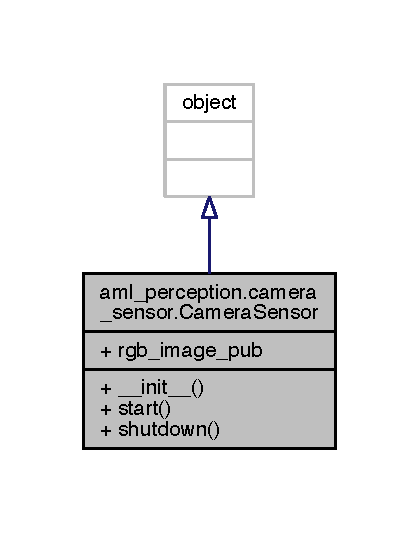
\includegraphics[width=198pt]{classaml__perception_1_1camera__sensor_1_1_camera_sensor__inherit__graph}
\end{center}
\end{figure}


Collaboration diagram for aml\-\_\-perception.\-camera\-\_\-sensor.\-Camera\-Sensor\-:
\nopagebreak
\begin{figure}[H]
\begin{center}
\leavevmode
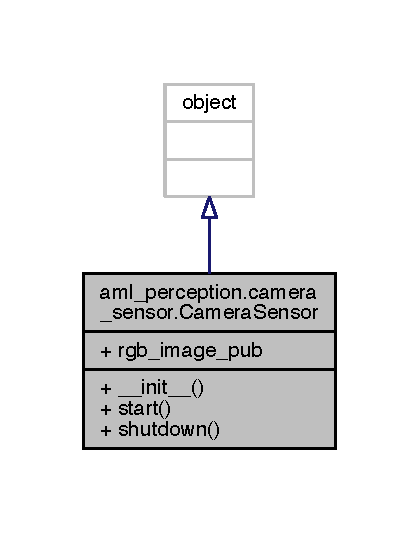
\includegraphics[width=198pt]{classaml__perception_1_1camera__sensor_1_1_camera_sensor__coll__graph}
\end{center}
\end{figure}
\subsection*{Public Member Functions}
\begin{DoxyCompactItemize}
\item 
\hypertarget{classaml__perception_1_1camera__sensor_1_1_camera_sensor_a21adf5c3740d47e8fb55c932e924618d}{def {\bfseries \-\_\-\-\_\-init\-\_\-\-\_\-}}\label{classaml__perception_1_1camera__sensor_1_1_camera_sensor_a21adf5c3740d47e8fb55c932e924618d}

\item 
\hypertarget{classaml__perception_1_1camera__sensor_1_1_camera_sensor_a08a06c82a0528c0462a49ec93db4dc0b}{def {\bfseries start}}\label{classaml__perception_1_1camera__sensor_1_1_camera_sensor_a08a06c82a0528c0462a49ec93db4dc0b}

\item 
\hypertarget{classaml__perception_1_1camera__sensor_1_1_camera_sensor_a95227671ed4cf14c09493d81bc619ea7}{def {\bfseries shutdown}}\label{classaml__perception_1_1camera__sensor_1_1_camera_sensor_a95227671ed4cf14c09493d81bc619ea7}

\item 
\hypertarget{classaml__perception_1_1camera__sensor_1_1_camera_sensor_adfbd28ea71c000f8ea5fed25868fb15f}{def {\bfseries set\-\_\-intrinsics}}\label{classaml__perception_1_1camera__sensor_1_1_camera_sensor_adfbd28ea71c000f8ea5fed25868fb15f}

\item 
\hypertarget{classaml__perception_1_1camera__sensor_1_1_camera_sensor_a57e0a5307a84544f0c0c5f8f1c0bc86b}{def {\bfseries intrinsics}}\label{classaml__perception_1_1camera__sensor_1_1_camera_sensor_a57e0a5307a84544f0c0c5f8f1c0bc86b}

\item 
\hypertarget{classaml__perception_1_1camera__sensor_1_1_camera_sensor_a0a599df52837dc5fc2debac009cbab99}{def {\bfseries rgb\-\_\-image}}\label{classaml__perception_1_1camera__sensor_1_1_camera_sensor_a0a599df52837dc5fc2debac009cbab99}

\item 
\hypertarget{classaml__perception_1_1camera__sensor_1_1_camera_sensor_ad77338064fe84b1932656006fdf5f366}{def {\bfseries depth\-\_\-image}}\label{classaml__perception_1_1camera__sensor_1_1_camera_sensor_ad77338064fe84b1932656006fdf5f366}

\item 
\hypertarget{classaml__perception_1_1camera__sensor_1_1_camera_sensor_abcd2dd8b9c56b814fccc4ae487835962}{def {\bfseries cloud}}\label{classaml__perception_1_1camera__sensor_1_1_camera_sensor_abcd2dd8b9c56b814fccc4ae487835962}

\item 
def \hyperlink{classaml__perception_1_1camera__sensor_1_1_camera_sensor_aa13c3fd9edecf042fb0a63daa1b2fc9a}{deproject}
\item 
def \hyperlink{classaml__perception_1_1camera__sensor_1_1_camera_sensor_a12f9efec439335da2874a9be29c63271}{project}
\end{DoxyCompactItemize}


\subsection{Member Function Documentation}
\hypertarget{classaml__perception_1_1camera__sensor_1_1_camera_sensor_aa13c3fd9edecf042fb0a63daa1b2fc9a}{\index{aml\-\_\-perception\-::camera\-\_\-sensor\-::\-Camera\-Sensor@{aml\-\_\-perception\-::camera\-\_\-sensor\-::\-Camera\-Sensor}!deproject@{deproject}}
\index{deproject@{deproject}!aml_perception::camera_sensor::CameraSensor@{aml\-\_\-perception\-::camera\-\_\-sensor\-::\-Camera\-Sensor}}
\subsubsection[{deproject}]{\setlength{\rightskip}{0pt plus 5cm}def aml\-\_\-perception.\-camera\-\_\-sensor.\-Camera\-Sensor.\-deproject (
\begin{DoxyParamCaption}
\item[{}]{self, }
\item[{}]{depth\-\_\-image}
\end{DoxyParamCaption}
)}}\label{classaml__perception_1_1camera__sensor_1_1_camera_sensor_aa13c3fd9edecf042fb0a63daa1b2fc9a}
\begin{DoxyVerb}Deprojects a depth image (2D numpy float array) into a point cloud
Params:

depth_image: (HxW numpy array of floats) 2D depth image to project
Returns:
3xN numpy float array of 3D points
\end{DoxyVerb}
 \hypertarget{classaml__perception_1_1camera__sensor_1_1_camera_sensor_a12f9efec439335da2874a9be29c63271}{\index{aml\-\_\-perception\-::camera\-\_\-sensor\-::\-Camera\-Sensor@{aml\-\_\-perception\-::camera\-\_\-sensor\-::\-Camera\-Sensor}!project@{project}}
\index{project@{project}!aml_perception::camera_sensor::CameraSensor@{aml\-\_\-perception\-::camera\-\_\-sensor\-::\-Camera\-Sensor}}
\subsubsection[{project}]{\setlength{\rightskip}{0pt plus 5cm}def aml\-\_\-perception.\-camera\-\_\-sensor.\-Camera\-Sensor.\-project (
\begin{DoxyParamCaption}
\item[{}]{self, }
\item[{}]{points}
\end{DoxyParamCaption}
)}}\label{classaml__perception_1_1camera__sensor_1_1_camera_sensor_a12f9efec439335da2874a9be29c63271}
\begin{DoxyVerb}Projects a set of points into the camera given by these parameters

Params:
points: (3xN numpy array of floats) 3D points to project
Returns:
2xN numpy float array of 2D image coordinates
1xN binary numpy array indicating whether or not point projected outside of image
\end{DoxyVerb}
 

The documentation for this class was generated from the following file\-:\begin{DoxyCompactItemize}
\item 
aml\-\_\-perception/src/aml\-\_\-perception/camera\-\_\-sensor.\-py\end{DoxyCompactItemize}

\hypertarget{classscripts_1_1collect__gravity__comp__data_1_1_collect_gravity_comp_data}{}\section{scripts.\+collect\+\_\+gravity\+\_\+comp\+\_\+data.\+Collect\+Gravity\+Comp\+Data Class Reference}
\label{classscripts_1_1collect__gravity__comp__data_1_1_collect_gravity_comp_data}\index{scripts.\+collect\+\_\+gravity\+\_\+comp\+\_\+data.\+Collect\+Gravity\+Comp\+Data@{scripts.\+collect\+\_\+gravity\+\_\+comp\+\_\+data.\+Collect\+Gravity\+Comp\+Data}}


Collaboration diagram for scripts.\+collect\+\_\+gravity\+\_\+comp\+\_\+data.\+Collect\+Gravity\+Comp\+Data\+:\nopagebreak
\begin{figure}[H]
\begin{center}
\leavevmode
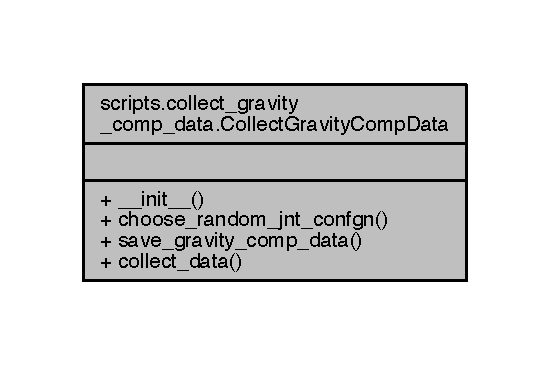
\includegraphics[width=264pt]{classscripts_1_1collect__gravity__comp__data_1_1_collect_gravity_comp_data__coll__graph}
\end{center}
\end{figure}
\subsection*{Public Member Functions}
\begin{DoxyCompactItemize}
\item 
\hypertarget{classscripts_1_1collect__gravity__comp__data_1_1_collect_gravity_comp_data_ac59a395138aef9b4c6b299eae0b973cf}{}\label{classscripts_1_1collect__gravity__comp__data_1_1_collect_gravity_comp_data_ac59a395138aef9b4c6b299eae0b973cf} 
def {\bfseries \+\_\+\+\_\+init\+\_\+\+\_\+} (self, robot\+\_\+interface, data\+\_\+cnt=10, sample\+\_\+rate=50)
\item 
\hypertarget{classscripts_1_1collect__gravity__comp__data_1_1_collect_gravity_comp_data_a5bbbfd37bc8de83b7b1c05fd04d18033}{}\label{classscripts_1_1collect__gravity__comp__data_1_1_collect_gravity_comp_data_a5bbbfd37bc8de83b7b1c05fd04d18033} 
def {\bfseries choose\+\_\+random\+\_\+jnt\+\_\+confgn} (self)
\item 
\hypertarget{classscripts_1_1collect__gravity__comp__data_1_1_collect_gravity_comp_data_a4c507f0db34276add5fba13a27b20d2f}{}\label{classscripts_1_1collect__gravity__comp__data_1_1_collect_gravity_comp_data_a4c507f0db34276add5fba13a27b20d2f} 
def {\bfseries save\+\_\+gravity\+\_\+comp\+\_\+data} (self, event)
\item 
\hypertarget{classscripts_1_1collect__gravity__comp__data_1_1_collect_gravity_comp_data_a27cb410f0fb3cbba3bab6d23b4f35dd8}{}\label{classscripts_1_1collect__gravity__comp__data_1_1_collect_gravity_comp_data_a27cb410f0fb3cbba3bab6d23b4f35dd8} 
def {\bfseries collect\+\_\+data} (self)
\end{DoxyCompactItemize}


The documentation for this class was generated from the following file\+:\begin{DoxyCompactItemize}
\item 
aml\+\_\+data\+\_\+collec\+\_\+utils/scripts/collect\+\_\+gravity\+\_\+comp\+\_\+data.\+py\end{DoxyCompactItemize}

\hypertarget{classscripts_1_1collect__poke__data_1_1_collect_poke_data}{}\section{scripts.\+collect\+\_\+poke\+\_\+data.\+Collect\+Poke\+Data Class Reference}
\label{classscripts_1_1collect__poke__data_1_1_collect_poke_data}\index{scripts.\+collect\+\_\+poke\+\_\+data.\+Collect\+Poke\+Data@{scripts.\+collect\+\_\+poke\+\_\+data.\+Collect\+Poke\+Data}}


Collaboration diagram for scripts.\+collect\+\_\+poke\+\_\+data.\+Collect\+Poke\+Data\+:\nopagebreak
\begin{figure}[H]
\begin{center}
\leavevmode
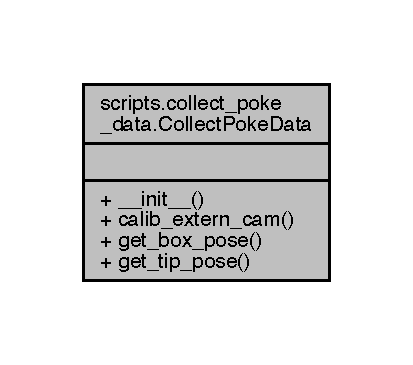
\includegraphics[width=198pt]{classscripts_1_1collect__poke__data_1_1_collect_poke_data__coll__graph}
\end{center}
\end{figure}
\subsection*{Public Member Functions}
\begin{DoxyCompactItemize}
\item 
\hypertarget{classscripts_1_1collect__poke__data_1_1_collect_poke_data_a949ee1345c3d5e23944cebb1c565b65c}{}\label{classscripts_1_1collect__poke__data_1_1_collect_poke_data_a949ee1345c3d5e23944cebb1c565b65c} 
def {\bfseries \+\_\+\+\_\+init\+\_\+\+\_\+} (self, robot\+\_\+interface, box\+\_\+config=B\+O\+X\+\_\+\+T\+Y\+P\+E\+\_\+1)
\item 
\hypertarget{classscripts_1_1collect__poke__data_1_1_collect_poke_data_acd76f6287f20334cf672df0b8112ae04}{}\label{classscripts_1_1collect__poke__data_1_1_collect_poke_data_acd76f6287f20334cf672df0b8112ae04} 
def {\bfseries calib\+\_\+extern\+\_\+cam} (self)
\item 
\hypertarget{classscripts_1_1collect__poke__data_1_1_collect_poke_data_a31e56ec91a9529fcf04e5c85ead5d82b}{}\label{classscripts_1_1collect__poke__data_1_1_collect_poke_data_a31e56ec91a9529fcf04e5c85ead5d82b} 
def {\bfseries get\+\_\+box\+\_\+pose} (self)
\item 
\hypertarget{classscripts_1_1collect__poke__data_1_1_collect_poke_data_afc60bf2012d30cc87ec83c4efe9031ee}{}\label{classscripts_1_1collect__poke__data_1_1_collect_poke_data_afc60bf2012d30cc87ec83c4efe9031ee} 
def {\bfseries get\+\_\+tip\+\_\+pose} (self)
\end{DoxyCompactItemize}


The documentation for this class was generated from the following file\+:\begin{DoxyCompactItemize}
\item 
aml\+\_\+data\+\_\+collec\+\_\+utils/scripts/collect\+\_\+poke\+\_\+data.\+py\end{DoxyCompactItemize}

\hypertarget{classaml__ctrl_1_1controller_1_1_controller}{\section{aml\-\_\-ctrl.\-controller.\-Controller Class Reference}
\label{classaml__ctrl_1_1controller_1_1_controller}\index{aml\-\_\-ctrl.\-controller.\-Controller@{aml\-\_\-ctrl.\-controller.\-Controller}}
}


Inheritance diagram for aml\-\_\-ctrl.\-controller.\-Controller\-:
\nopagebreak
\begin{figure}[H]
\begin{center}
\leavevmode
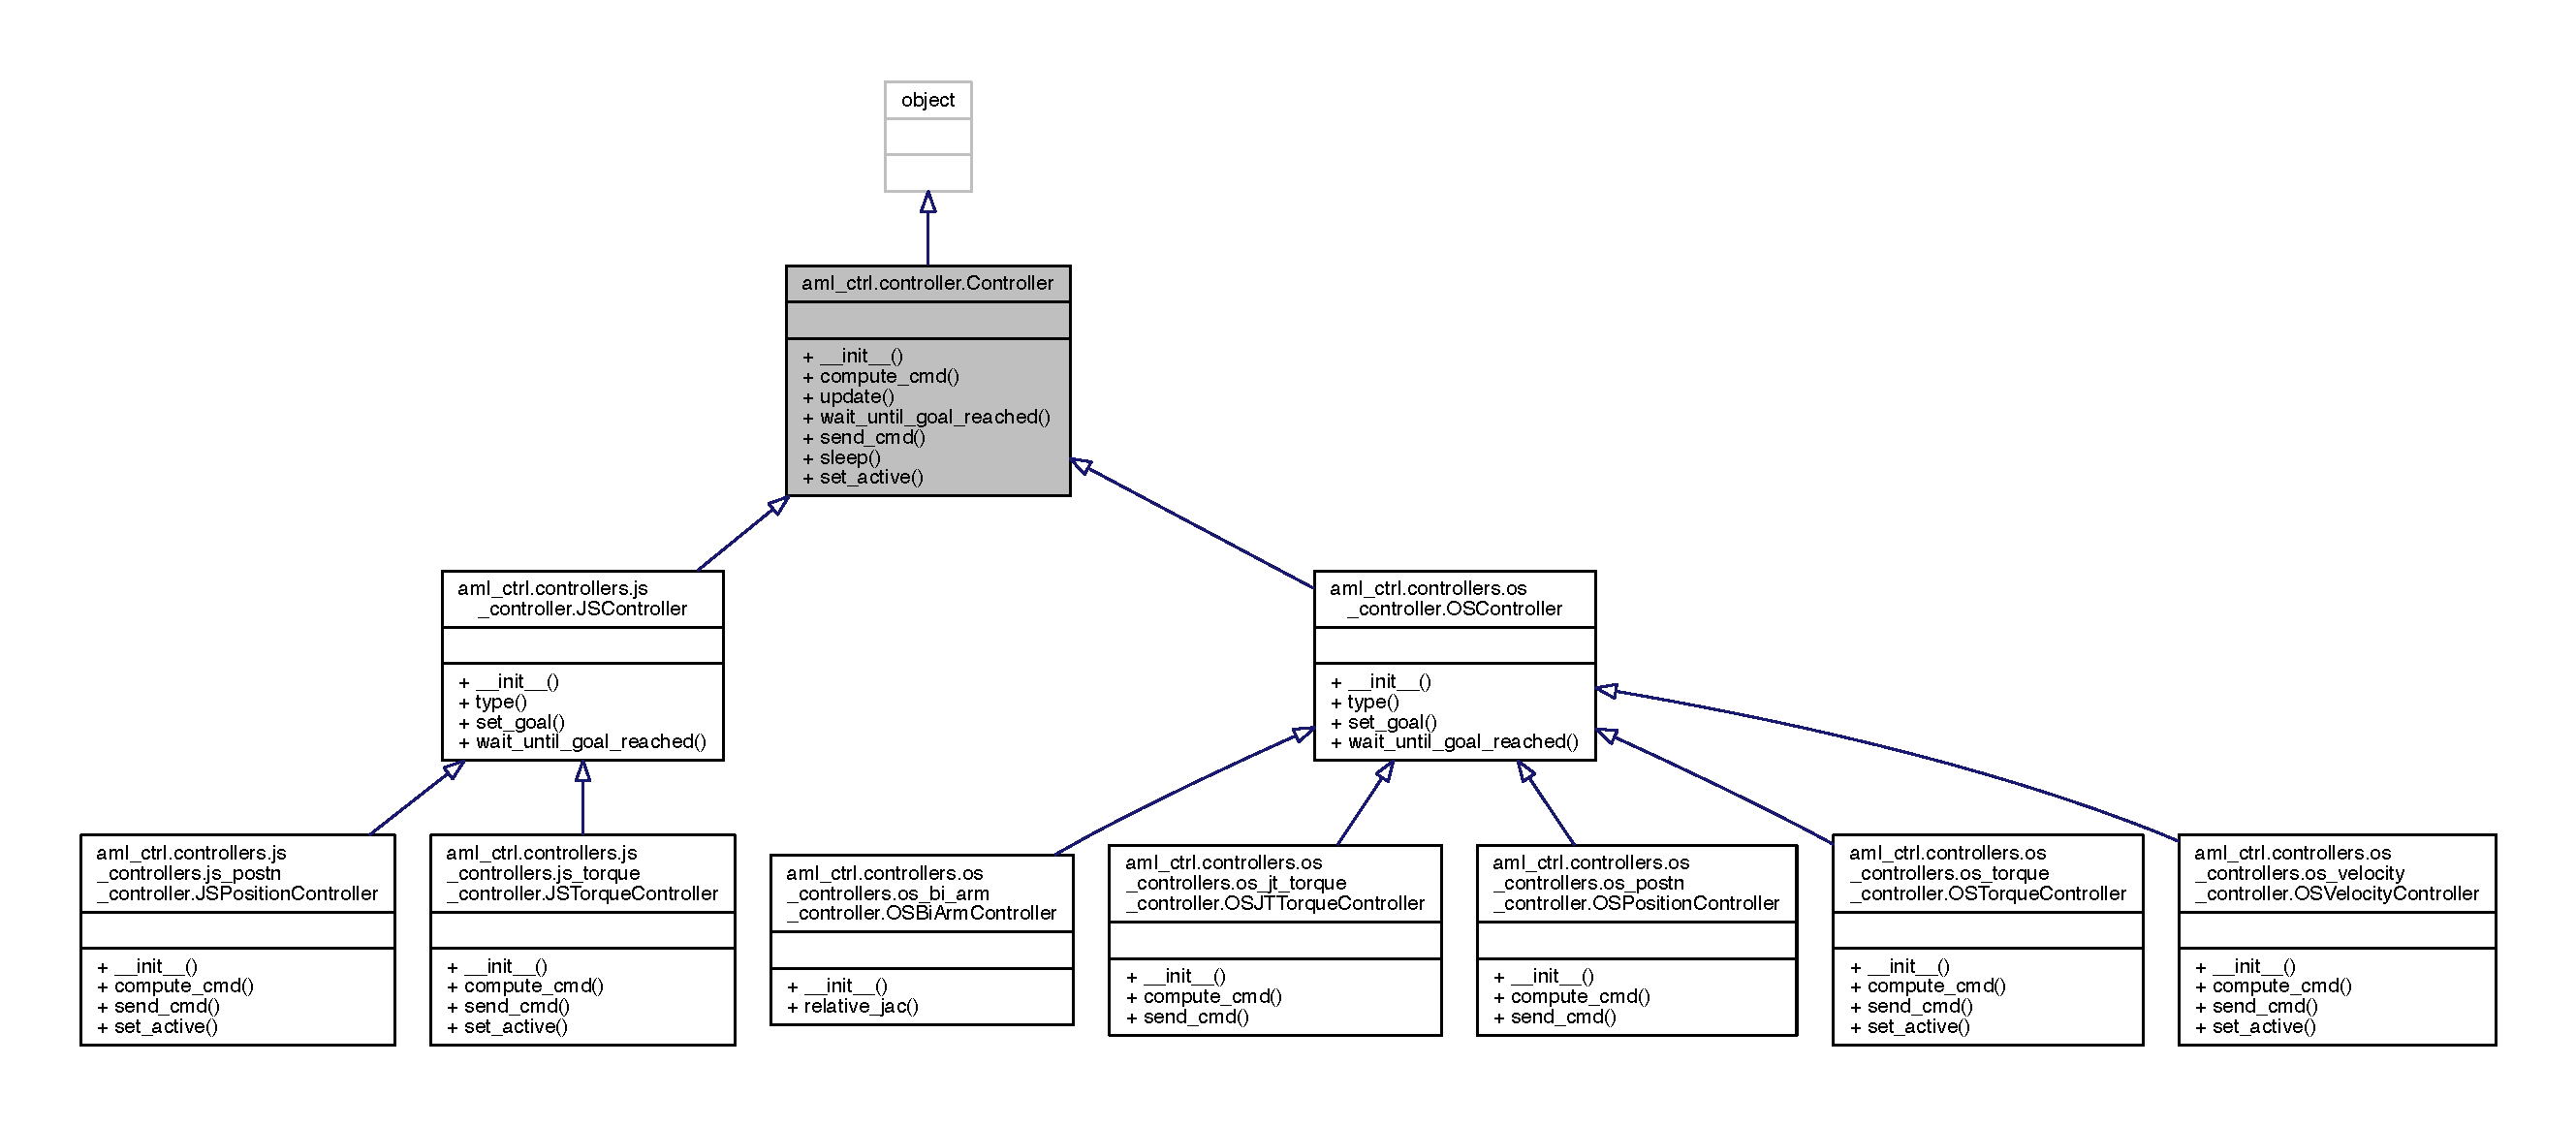
\includegraphics[width=350pt]{classaml__ctrl_1_1controller_1_1_controller__inherit__graph}
\end{center}
\end{figure}


Collaboration diagram for aml\-\_\-ctrl.\-controller.\-Controller\-:
\nopagebreak
\begin{figure}[H]
\begin{center}
\leavevmode
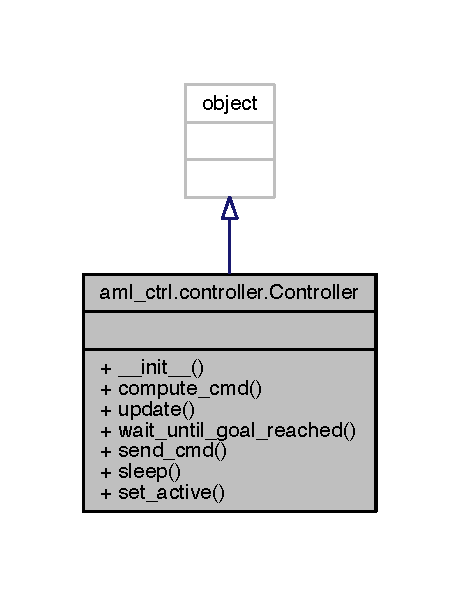
\includegraphics[width=218pt]{classaml__ctrl_1_1controller_1_1_controller__coll__graph}
\end{center}
\end{figure}
\subsection*{Public Member Functions}
\begin{DoxyCompactItemize}
\item 
\hypertarget{classaml__ctrl_1_1controller_1_1_controller_ac1a1888ac43afe5d53e3120d3370db9e}{def {\bfseries \-\_\-\-\_\-init\-\_\-\-\_\-}}\label{classaml__ctrl_1_1controller_1_1_controller_ac1a1888ac43afe5d53e3120d3370db9e}

\item 
\hypertarget{classaml__ctrl_1_1controller_1_1_controller_aace14d69a66dfa391a7d1c8d137b4fe2}{def {\bfseries compute\-\_\-cmd}}\label{classaml__ctrl_1_1controller_1_1_controller_aace14d69a66dfa391a7d1c8d137b4fe2}

\item 
\hypertarget{classaml__ctrl_1_1controller_1_1_controller_ad6f4761cc5211316e70a424472748a2a}{def {\bfseries update}}\label{classaml__ctrl_1_1controller_1_1_controller_ad6f4761cc5211316e70a424472748a2a}

\item 
\hypertarget{classaml__ctrl_1_1controller_1_1_controller_a06f4b5748924ca72a3a6f349370122cd}{def {\bfseries wait\-\_\-until\-\_\-goal\-\_\-reached}}\label{classaml__ctrl_1_1controller_1_1_controller_a06f4b5748924ca72a3a6f349370122cd}

\item 
\hypertarget{classaml__ctrl_1_1controller_1_1_controller_a341e4994f8a876aef85601d622afc968}{def {\bfseries send\-\_\-cmd}}\label{classaml__ctrl_1_1controller_1_1_controller_a341e4994f8a876aef85601d622afc968}

\item 
\hypertarget{classaml__ctrl_1_1controller_1_1_controller_a4047e0ef3a57caf51b599f6d0dc78fe1}{def {\bfseries sleep}}\label{classaml__ctrl_1_1controller_1_1_controller_a4047e0ef3a57caf51b599f6d0dc78fe1}

\item 
\hypertarget{classaml__ctrl_1_1controller_1_1_controller_ab3cf24f3dae223949e893bc61595c89e}{def {\bfseries set\-\_\-active}}\label{classaml__ctrl_1_1controller_1_1_controller_ab3cf24f3dae223949e893bc61595c89e}

\item 
\hypertarget{classaml__ctrl_1_1controller_1_1_controller_a1952a0675d40dee30d917b3f00fe555f}{def {\bfseries is\-\_\-active}}\label{classaml__ctrl_1_1controller_1_1_controller_a1952a0675d40dee30d917b3f00fe555f}

\end{DoxyCompactItemize}


The documentation for this class was generated from the following file\-:\begin{DoxyCompactItemize}
\item 
aml\-\_\-ctrl/src/aml\-\_\-ctrl/controller.\-py\end{DoxyCompactItemize}

\hypertarget{classaml__robot_1_1box2d_1_1data__manager_1_1_data_manager}{}\section{aml\+\_\+robot.\+box2d.\+data\+\_\+manager.\+Data\+Manager Class Reference}
\label{classaml__robot_1_1box2d_1_1data__manager_1_1_data_manager}\index{aml\+\_\+robot.\+box2d.\+data\+\_\+manager.\+Data\+Manager@{aml\+\_\+robot.\+box2d.\+data\+\_\+manager.\+Data\+Manager}}


Inheritance diagram for aml\+\_\+robot.\+box2d.\+data\+\_\+manager.\+Data\+Manager\+:\nopagebreak
\begin{figure}[H]
\begin{center}
\leavevmode
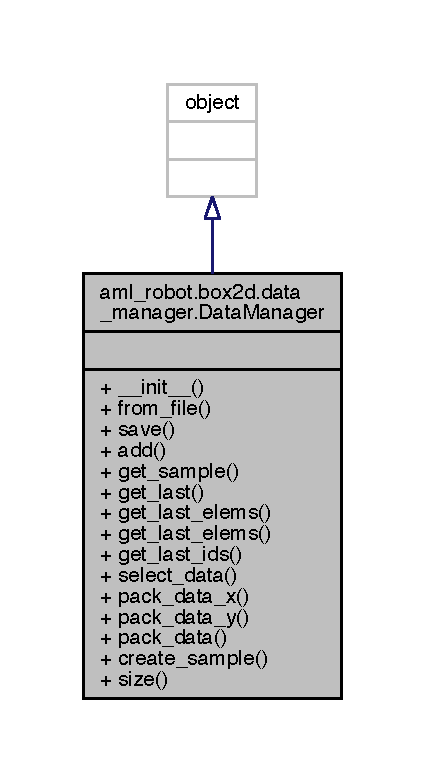
\includegraphics[width=204pt]{classaml__robot_1_1box2d_1_1data__manager_1_1_data_manager__inherit__graph}
\end{center}
\end{figure}


Collaboration diagram for aml\+\_\+robot.\+box2d.\+data\+\_\+manager.\+Data\+Manager\+:\nopagebreak
\begin{figure}[H]
\begin{center}
\leavevmode
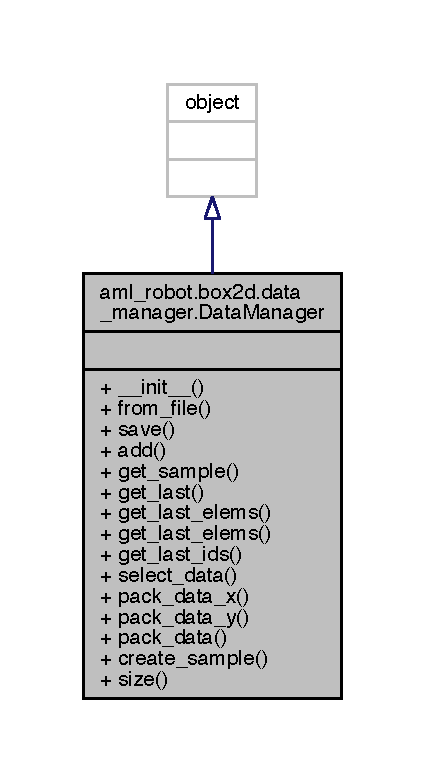
\includegraphics[width=204pt]{classaml__robot_1_1box2d_1_1data__manager_1_1_data_manager__coll__graph}
\end{center}
\end{figure}
\subsection*{Public Member Functions}
\begin{DoxyCompactItemize}
\item 
\hypertarget{classaml__robot_1_1box2d_1_1data__manager_1_1_data_manager_aa0580187539e82c3ceac6917bffe62fa}{}\label{classaml__robot_1_1box2d_1_1data__manager_1_1_data_manager_aa0580187539e82c3ceac6917bffe62fa} 
def {\bfseries \+\_\+\+\_\+init\+\_\+\+\_\+} (self, data=\mbox{[}$\,$\mbox{]})
\item 
\hypertarget{classaml__robot_1_1box2d_1_1data__manager_1_1_data_manager_a400cf525806b262ec07a4432886ce611}{}\label{classaml__robot_1_1box2d_1_1data__manager_1_1_data_manager_a400cf525806b262ec07a4432886ce611} 
def {\bfseries from\+\_\+file} (cls, filename)
\item 
\hypertarget{classaml__robot_1_1box2d_1_1data__manager_1_1_data_manager_a1d5d0230feeab6bd931b3fcebbf7f5f8}{}\label{classaml__robot_1_1box2d_1_1data__manager_1_1_data_manager_a1d5d0230feeab6bd931b3fcebbf7f5f8} 
def {\bfseries save} (self, filename)
\item 
\hypertarget{classaml__robot_1_1box2d_1_1data__manager_1_1_data_manager_a00530313dc94c0c8dd2da7eb50d3739e}{}\label{classaml__robot_1_1box2d_1_1data__manager_1_1_data_manager_a00530313dc94c0c8dd2da7eb50d3739e} 
def {\bfseries add} (self, sample)
\item 
\hypertarget{classaml__robot_1_1box2d_1_1data__manager_1_1_data_manager_a2ccfb6f0938fccc05d6c44670d62e82e}{}\label{classaml__robot_1_1box2d_1_1data__manager_1_1_data_manager_a2ccfb6f0938fccc05d6c44670d62e82e} 
def {\bfseries get\+\_\+sample} (self, idx, key)
\item 
\hypertarget{classaml__robot_1_1box2d_1_1data__manager_1_1_data_manager_a65e78ddd432d63b011c9daffa16270fb}{}\label{classaml__robot_1_1box2d_1_1data__manager_1_1_data_manager_a65e78ddd432d63b011c9daffa16270fb} 
def {\bfseries get\+\_\+last} (self)
\item 
\hypertarget{classaml__robot_1_1box2d_1_1data__manager_1_1_data_manager_a229d07bd1289ae076b6d85006fb79317}{}\label{classaml__robot_1_1box2d_1_1data__manager_1_1_data_manager_a229d07bd1289ae076b6d85006fb79317} 
def {\bfseries get\+\_\+last\+\_\+elems} (self, n=1)
\item 
\hypertarget{classaml__robot_1_1box2d_1_1data__manager_1_1_data_manager_a229d07bd1289ae076b6d85006fb79317}{}\label{classaml__robot_1_1box2d_1_1data__manager_1_1_data_manager_a229d07bd1289ae076b6d85006fb79317} 
def {\bfseries get\+\_\+last\+\_\+elems} (self, n=1)
\item 
\hypertarget{classaml__robot_1_1box2d_1_1data__manager_1_1_data_manager_a4f5a35574b483916068562d4d9f9c19c}{}\label{classaml__robot_1_1box2d_1_1data__manager_1_1_data_manager_a4f5a35574b483916068562d4d9f9c19c} 
def {\bfseries get\+\_\+last\+\_\+ids} (self, n=1)
\item 
\hypertarget{classaml__robot_1_1box2d_1_1data__manager_1_1_data_manager_aa573ee39665d43261bb768c1c3c1cb64}{}\label{classaml__robot_1_1box2d_1_1data__manager_1_1_data_manager_aa573ee39665d43261bb768c1c3c1cb64} 
def {\bfseries select\+\_\+data} (self, ids=None)
\item 
\hypertarget{classaml__robot_1_1box2d_1_1data__manager_1_1_data_manager_a3351b75171e381a07c89fabb723c770b}{}\label{classaml__robot_1_1box2d_1_1data__manager_1_1_data_manager_a3351b75171e381a07c89fabb723c770b} 
def {\bfseries pack\+\_\+data\+\_\+x} (self, keys, ids=None)
\item 
\hypertarget{classaml__robot_1_1box2d_1_1data__manager_1_1_data_manager_a73f284159c9b215bf6884565caf0f601}{}\label{classaml__robot_1_1box2d_1_1data__manager_1_1_data_manager_a73f284159c9b215bf6884565caf0f601} 
def {\bfseries pack\+\_\+data\+\_\+y} (self, ids=None)
\item 
\hypertarget{classaml__robot_1_1box2d_1_1data__manager_1_1_data_manager_ad9975a5ada92b83489e2ccd80db88f13}{}\label{classaml__robot_1_1box2d_1_1data__manager_1_1_data_manager_ad9975a5ada92b83489e2ccd80db88f13} 
def {\bfseries pack\+\_\+data} (self, keys, ids=None)
\item 
\hypertarget{classaml__robot_1_1box2d_1_1data__manager_1_1_data_manager_a4146de256982fba71b91a46a9117ae60}{}\label{classaml__robot_1_1box2d_1_1data__manager_1_1_data_manager_a4146de256982fba71b91a46a9117ae60} 
def {\bfseries create\+\_\+sample} (self)
\item 
\hypertarget{classaml__robot_1_1box2d_1_1data__manager_1_1_data_manager_aaa5cac201a4804c05c4ad9ee950aca33}{}\label{classaml__robot_1_1box2d_1_1data__manager_1_1_data_manager_aaa5cac201a4804c05c4ad9ee950aca33} 
def {\bfseries size} (self)
\end{DoxyCompactItemize}


The documentation for this class was generated from the following file\+:\begin{DoxyCompactItemize}
\item 
aml\+\_\+robot/src/aml\+\_\+robot/box2d/data\+\_\+manager.\+py\end{DoxyCompactItemize}

\hypertarget{classaml__lfd_1_1ilqr_1_1ilqr__traj__follow_1_1_d_d_p___traj_follow_class}{\section{aml\-\_\-lfd.\-ilqr.\-ilqr\-\_\-traj\-\_\-follow.\-D\-D\-P\-\_\-\-Traj\-Follow\-Class Class Reference}
\label{classaml__lfd_1_1ilqr_1_1ilqr__traj__follow_1_1_d_d_p___traj_follow_class}\index{aml\-\_\-lfd.\-ilqr.\-ilqr\-\_\-traj\-\_\-follow.\-D\-D\-P\-\_\-\-Traj\-Follow\-Class@{aml\-\_\-lfd.\-ilqr.\-ilqr\-\_\-traj\-\_\-follow.\-D\-D\-P\-\_\-\-Traj\-Follow\-Class}}
}


Collaboration diagram for aml\-\_\-lfd.\-ilqr.\-ilqr\-\_\-traj\-\_\-follow.\-D\-D\-P\-\_\-\-Traj\-Follow\-Class\-:\nopagebreak
\begin{figure}[H]
\begin{center}
\leavevmode
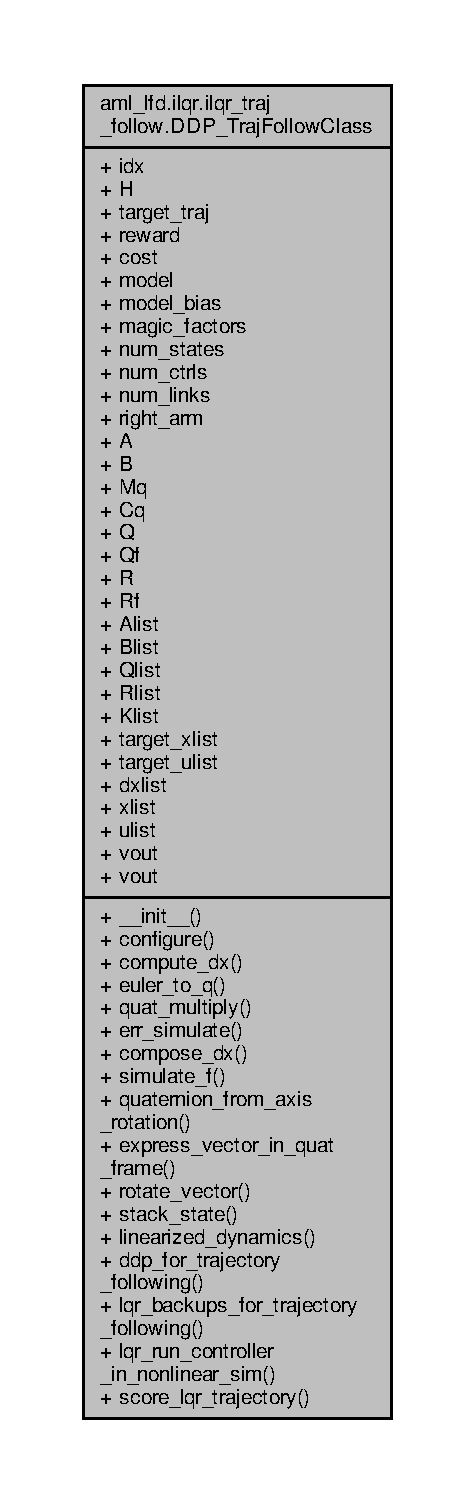
\includegraphics[height=550pt]{classaml__lfd_1_1ilqr_1_1ilqr__traj__follow_1_1_d_d_p___traj_follow_class__coll__graph}
\end{center}
\end{figure}
\subsection*{Public Member Functions}
\begin{DoxyCompactItemize}
\item 
\hypertarget{classaml__lfd_1_1ilqr_1_1ilqr__traj__follow_1_1_d_d_p___traj_follow_class_ad7fc5b47422623c1369ef622a30ba654}{def {\bfseries \-\_\-\-\_\-init\-\_\-\-\_\-}}\label{classaml__lfd_1_1ilqr_1_1ilqr__traj__follow_1_1_d_d_p___traj_follow_class_ad7fc5b47422623c1369ef622a30ba654}

\item 
\hypertarget{classaml__lfd_1_1ilqr_1_1ilqr__traj__follow_1_1_d_d_p___traj_follow_class_ac3673e1d7138eade9bcc0e12e8546322}{def {\bfseries configure}}\label{classaml__lfd_1_1ilqr_1_1ilqr__traj__follow_1_1_d_d_p___traj_follow_class_ac3673e1d7138eade9bcc0e12e8546322}

\item 
\hypertarget{classaml__lfd_1_1ilqr_1_1ilqr__traj__follow_1_1_d_d_p___traj_follow_class_aed985f043586a1740a0181d331f53176}{def {\bfseries compute\-\_\-dx}}\label{classaml__lfd_1_1ilqr_1_1ilqr__traj__follow_1_1_d_d_p___traj_follow_class_aed985f043586a1740a0181d331f53176}

\item 
\hypertarget{classaml__lfd_1_1ilqr_1_1ilqr__traj__follow_1_1_d_d_p___traj_follow_class_ad2e783809690f057364e87eaa52f48ab}{def {\bfseries euler\-\_\-to\-\_\-q}}\label{classaml__lfd_1_1ilqr_1_1ilqr__traj__follow_1_1_d_d_p___traj_follow_class_ad2e783809690f057364e87eaa52f48ab}

\item 
\hypertarget{classaml__lfd_1_1ilqr_1_1ilqr__traj__follow_1_1_d_d_p___traj_follow_class_a33165af92cd027dea290adda63a6b036}{def {\bfseries quat\-\_\-multiply}}\label{classaml__lfd_1_1ilqr_1_1ilqr__traj__follow_1_1_d_d_p___traj_follow_class_a33165af92cd027dea290adda63a6b036}

\item 
\hypertarget{classaml__lfd_1_1ilqr_1_1ilqr__traj__follow_1_1_d_d_p___traj_follow_class_a7f873bf434749da8e00780f991dd875a}{def {\bfseries err\-\_\-simulate}}\label{classaml__lfd_1_1ilqr_1_1ilqr__traj__follow_1_1_d_d_p___traj_follow_class_a7f873bf434749da8e00780f991dd875a}

\item 
\hypertarget{classaml__lfd_1_1ilqr_1_1ilqr__traj__follow_1_1_d_d_p___traj_follow_class_afc28b6ddc1d262b1d5e11312e880db30}{def {\bfseries compose\-\_\-dx}}\label{classaml__lfd_1_1ilqr_1_1ilqr__traj__follow_1_1_d_d_p___traj_follow_class_afc28b6ddc1d262b1d5e11312e880db30}

\item 
\hypertarget{classaml__lfd_1_1ilqr_1_1ilqr__traj__follow_1_1_d_d_p___traj_follow_class_ac0d8f0c54d196a70822308a3b3a3150f}{def {\bfseries simulate\-\_\-f}}\label{classaml__lfd_1_1ilqr_1_1ilqr__traj__follow_1_1_d_d_p___traj_follow_class_ac0d8f0c54d196a70822308a3b3a3150f}

\item 
\hypertarget{classaml__lfd_1_1ilqr_1_1ilqr__traj__follow_1_1_d_d_p___traj_follow_class_abd87fb33b984bf16a7b8a22e156ad9bd}{def {\bfseries quaternion\-\_\-from\-\_\-axis\-\_\-rotation}}\label{classaml__lfd_1_1ilqr_1_1ilqr__traj__follow_1_1_d_d_p___traj_follow_class_abd87fb33b984bf16a7b8a22e156ad9bd}

\item 
\hypertarget{classaml__lfd_1_1ilqr_1_1ilqr__traj__follow_1_1_d_d_p___traj_follow_class_ace91aea7502ef0c2923f74b16e6c5e11}{def {\bfseries express\-\_\-vector\-\_\-in\-\_\-quat\-\_\-frame}}\label{classaml__lfd_1_1ilqr_1_1ilqr__traj__follow_1_1_d_d_p___traj_follow_class_ace91aea7502ef0c2923f74b16e6c5e11}

\item 
\hypertarget{classaml__lfd_1_1ilqr_1_1ilqr__traj__follow_1_1_d_d_p___traj_follow_class_af6bb5e31fe445276d683d947a444d557}{def {\bfseries rotate\-\_\-vector}}\label{classaml__lfd_1_1ilqr_1_1ilqr__traj__follow_1_1_d_d_p___traj_follow_class_af6bb5e31fe445276d683d947a444d557}

\item 
\hypertarget{classaml__lfd_1_1ilqr_1_1ilqr__traj__follow_1_1_d_d_p___traj_follow_class_ae591b82eb361d4c870535bfe9cd3511e}{def {\bfseries stack\-\_\-state}}\label{classaml__lfd_1_1ilqr_1_1ilqr__traj__follow_1_1_d_d_p___traj_follow_class_ae591b82eb361d4c870535bfe9cd3511e}

\item 
\hypertarget{classaml__lfd_1_1ilqr_1_1ilqr__traj__follow_1_1_d_d_p___traj_follow_class_a0c9aed35c760850a40dce2504a8102fc}{def {\bfseries linearized\-\_\-dynamics}}\label{classaml__lfd_1_1ilqr_1_1ilqr__traj__follow_1_1_d_d_p___traj_follow_class_a0c9aed35c760850a40dce2504a8102fc}

\item 
\hypertarget{classaml__lfd_1_1ilqr_1_1ilqr__traj__follow_1_1_d_d_p___traj_follow_class_ad0160a37cf1558a94e5fe280ef363b0f}{def {\bfseries ddp\-\_\-for\-\_\-trajectory\-\_\-following}}\label{classaml__lfd_1_1ilqr_1_1ilqr__traj__follow_1_1_d_d_p___traj_follow_class_ad0160a37cf1558a94e5fe280ef363b0f}

\item 
\hypertarget{classaml__lfd_1_1ilqr_1_1ilqr__traj__follow_1_1_d_d_p___traj_follow_class_a26cfeaef8f2b3c3772e90eafd5550dd2}{def {\bfseries lqr\-\_\-backups\-\_\-for\-\_\-trajectory\-\_\-following}}\label{classaml__lfd_1_1ilqr_1_1ilqr__traj__follow_1_1_d_d_p___traj_follow_class_a26cfeaef8f2b3c3772e90eafd5550dd2}

\item 
\hypertarget{classaml__lfd_1_1ilqr_1_1ilqr__traj__follow_1_1_d_d_p___traj_follow_class_aaf416ec526fdccbbd0b19a57e9372d77}{def {\bfseries lqr\-\_\-run\-\_\-controller\-\_\-in\-\_\-nonlinear\-\_\-sim}}\label{classaml__lfd_1_1ilqr_1_1ilqr__traj__follow_1_1_d_d_p___traj_follow_class_aaf416ec526fdccbbd0b19a57e9372d77}

\item 
\hypertarget{classaml__lfd_1_1ilqr_1_1ilqr__traj__follow_1_1_d_d_p___traj_follow_class_a9459c23b6439beaeb095011e013d3c09}{def {\bfseries score\-\_\-lqr\-\_\-trajectory}}\label{classaml__lfd_1_1ilqr_1_1ilqr__traj__follow_1_1_d_d_p___traj_follow_class_a9459c23b6439beaeb095011e013d3c09}

\end{DoxyCompactItemize}
\subsection*{Public Attributes}
\begin{DoxyCompactItemize}
\item 
\hypertarget{classaml__lfd_1_1ilqr_1_1ilqr__traj__follow_1_1_d_d_p___traj_follow_class_a24d5d726678380440f768704b014d3cb}{{\bfseries idx}}\label{classaml__lfd_1_1ilqr_1_1ilqr__traj__follow_1_1_d_d_p___traj_follow_class_a24d5d726678380440f768704b014d3cb}

\item 
\hypertarget{classaml__lfd_1_1ilqr_1_1ilqr__traj__follow_1_1_d_d_p___traj_follow_class_af293f4032dae063fcef8b87db6f0755d}{{\bfseries H}}\label{classaml__lfd_1_1ilqr_1_1ilqr__traj__follow_1_1_d_d_p___traj_follow_class_af293f4032dae063fcef8b87db6f0755d}

\item 
\hypertarget{classaml__lfd_1_1ilqr_1_1ilqr__traj__follow_1_1_d_d_p___traj_follow_class_afa1787ffdca740b26dea0352871facaa}{{\bfseries target\-\_\-traj}}\label{classaml__lfd_1_1ilqr_1_1ilqr__traj__follow_1_1_d_d_p___traj_follow_class_afa1787ffdca740b26dea0352871facaa}

\item 
\hypertarget{classaml__lfd_1_1ilqr_1_1ilqr__traj__follow_1_1_d_d_p___traj_follow_class_af69890ed626d1d51fd0c0c9c90a07029}{{\bfseries reward}}\label{classaml__lfd_1_1ilqr_1_1ilqr__traj__follow_1_1_d_d_p___traj_follow_class_af69890ed626d1d51fd0c0c9c90a07029}

\item 
\hypertarget{classaml__lfd_1_1ilqr_1_1ilqr__traj__follow_1_1_d_d_p___traj_follow_class_afebda9c04f87f105838bbe8d0d459a9f}{{\bfseries cost}}\label{classaml__lfd_1_1ilqr_1_1ilqr__traj__follow_1_1_d_d_p___traj_follow_class_afebda9c04f87f105838bbe8d0d459a9f}

\item 
\hypertarget{classaml__lfd_1_1ilqr_1_1ilqr__traj__follow_1_1_d_d_p___traj_follow_class_a92ebe7f59db045d57fd0ec0dd5eb8233}{{\bfseries model}}\label{classaml__lfd_1_1ilqr_1_1ilqr__traj__follow_1_1_d_d_p___traj_follow_class_a92ebe7f59db045d57fd0ec0dd5eb8233}

\item 
\hypertarget{classaml__lfd_1_1ilqr_1_1ilqr__traj__follow_1_1_d_d_p___traj_follow_class_a9bbff6812b2bb4ad8498049c36c4456b}{{\bfseries model\-\_\-bias}}\label{classaml__lfd_1_1ilqr_1_1ilqr__traj__follow_1_1_d_d_p___traj_follow_class_a9bbff6812b2bb4ad8498049c36c4456b}

\item 
\hypertarget{classaml__lfd_1_1ilqr_1_1ilqr__traj__follow_1_1_d_d_p___traj_follow_class_a868566fc02ed89a173ed419e4e16f592}{{\bfseries magic\-\_\-factors}}\label{classaml__lfd_1_1ilqr_1_1ilqr__traj__follow_1_1_d_d_p___traj_follow_class_a868566fc02ed89a173ed419e4e16f592}

\item 
\hypertarget{classaml__lfd_1_1ilqr_1_1ilqr__traj__follow_1_1_d_d_p___traj_follow_class_ae474874e12f41dba69615a82c7a8cb60}{{\bfseries num\-\_\-states}}\label{classaml__lfd_1_1ilqr_1_1ilqr__traj__follow_1_1_d_d_p___traj_follow_class_ae474874e12f41dba69615a82c7a8cb60}

\item 
\hypertarget{classaml__lfd_1_1ilqr_1_1ilqr__traj__follow_1_1_d_d_p___traj_follow_class_a9c3bdb7c8a694200ad80c8c1aee526c2}{{\bfseries num\-\_\-ctrls}}\label{classaml__lfd_1_1ilqr_1_1ilqr__traj__follow_1_1_d_d_p___traj_follow_class_a9c3bdb7c8a694200ad80c8c1aee526c2}

\item 
\hypertarget{classaml__lfd_1_1ilqr_1_1ilqr__traj__follow_1_1_d_d_p___traj_follow_class_ab8ccf4574218a1a3e7126f27b3408789}{{\bfseries num\-\_\-links}}\label{classaml__lfd_1_1ilqr_1_1ilqr__traj__follow_1_1_d_d_p___traj_follow_class_ab8ccf4574218a1a3e7126f27b3408789}

\item 
\hypertarget{classaml__lfd_1_1ilqr_1_1ilqr__traj__follow_1_1_d_d_p___traj_follow_class_a50b099d5205a3fa99dbaacd3057cc148}{{\bfseries right\-\_\-arm}}\label{classaml__lfd_1_1ilqr_1_1ilqr__traj__follow_1_1_d_d_p___traj_follow_class_a50b099d5205a3fa99dbaacd3057cc148}

\item 
\hypertarget{classaml__lfd_1_1ilqr_1_1ilqr__traj__follow_1_1_d_d_p___traj_follow_class_ae5267f78b503df5d7ead70bfa2475e97}{{\bfseries A}}\label{classaml__lfd_1_1ilqr_1_1ilqr__traj__follow_1_1_d_d_p___traj_follow_class_ae5267f78b503df5d7ead70bfa2475e97}

\item 
\hypertarget{classaml__lfd_1_1ilqr_1_1ilqr__traj__follow_1_1_d_d_p___traj_follow_class_a785a4e091b777d2b31041be375a46a49}{{\bfseries B}}\label{classaml__lfd_1_1ilqr_1_1ilqr__traj__follow_1_1_d_d_p___traj_follow_class_a785a4e091b777d2b31041be375a46a49}

\item 
\hypertarget{classaml__lfd_1_1ilqr_1_1ilqr__traj__follow_1_1_d_d_p___traj_follow_class_a6d27ee9d34134d8d37f5cf3ebea59741}{{\bfseries Mq}}\label{classaml__lfd_1_1ilqr_1_1ilqr__traj__follow_1_1_d_d_p___traj_follow_class_a6d27ee9d34134d8d37f5cf3ebea59741}

\item 
\hypertarget{classaml__lfd_1_1ilqr_1_1ilqr__traj__follow_1_1_d_d_p___traj_follow_class_ae34c9104cc990dde3a60ac3bad1ca2e3}{{\bfseries Cq}}\label{classaml__lfd_1_1ilqr_1_1ilqr__traj__follow_1_1_d_d_p___traj_follow_class_ae34c9104cc990dde3a60ac3bad1ca2e3}

\item 
\hypertarget{classaml__lfd_1_1ilqr_1_1ilqr__traj__follow_1_1_d_d_p___traj_follow_class_a1d99f2916f1896bd424ba68a1f67e814}{{\bfseries Q}}\label{classaml__lfd_1_1ilqr_1_1ilqr__traj__follow_1_1_d_d_p___traj_follow_class_a1d99f2916f1896bd424ba68a1f67e814}

\item 
\hypertarget{classaml__lfd_1_1ilqr_1_1ilqr__traj__follow_1_1_d_d_p___traj_follow_class_a307ecd9fdbbab36d3bc067730e4fab64}{{\bfseries Qf}}\label{classaml__lfd_1_1ilqr_1_1ilqr__traj__follow_1_1_d_d_p___traj_follow_class_a307ecd9fdbbab36d3bc067730e4fab64}

\item 
\hypertarget{classaml__lfd_1_1ilqr_1_1ilqr__traj__follow_1_1_d_d_p___traj_follow_class_a6f4f259eada3a4e47f5a711747b1e342}{{\bfseries R}}\label{classaml__lfd_1_1ilqr_1_1ilqr__traj__follow_1_1_d_d_p___traj_follow_class_a6f4f259eada3a4e47f5a711747b1e342}

\item 
\hypertarget{classaml__lfd_1_1ilqr_1_1ilqr__traj__follow_1_1_d_d_p___traj_follow_class_abb529fb840b8d7ab8a4207e3f51e29c1}{{\bfseries Rf}}\label{classaml__lfd_1_1ilqr_1_1ilqr__traj__follow_1_1_d_d_p___traj_follow_class_abb529fb840b8d7ab8a4207e3f51e29c1}

\item 
\hypertarget{classaml__lfd_1_1ilqr_1_1ilqr__traj__follow_1_1_d_d_p___traj_follow_class_a61793e7ea328fb11752146fa5106c5e1}{{\bfseries Alist}}\label{classaml__lfd_1_1ilqr_1_1ilqr__traj__follow_1_1_d_d_p___traj_follow_class_a61793e7ea328fb11752146fa5106c5e1}

\item 
\hypertarget{classaml__lfd_1_1ilqr_1_1ilqr__traj__follow_1_1_d_d_p___traj_follow_class_ae5dbe5975a442e1e3f14467cf6d09968}{{\bfseries Blist}}\label{classaml__lfd_1_1ilqr_1_1ilqr__traj__follow_1_1_d_d_p___traj_follow_class_ae5dbe5975a442e1e3f14467cf6d09968}

\item 
\hypertarget{classaml__lfd_1_1ilqr_1_1ilqr__traj__follow_1_1_d_d_p___traj_follow_class_aa003fc26899988835cd9231b709f5e62}{{\bfseries Qlist}}\label{classaml__lfd_1_1ilqr_1_1ilqr__traj__follow_1_1_d_d_p___traj_follow_class_aa003fc26899988835cd9231b709f5e62}

\item 
\hypertarget{classaml__lfd_1_1ilqr_1_1ilqr__traj__follow_1_1_d_d_p___traj_follow_class_a769b8bb1bbd4803d742df4a124930cd0}{{\bfseries Rlist}}\label{classaml__lfd_1_1ilqr_1_1ilqr__traj__follow_1_1_d_d_p___traj_follow_class_a769b8bb1bbd4803d742df4a124930cd0}

\item 
\hypertarget{classaml__lfd_1_1ilqr_1_1ilqr__traj__follow_1_1_d_d_p___traj_follow_class_a9c06e5ea9a384bce048d5c7e3ddc8d93}{{\bfseries Klist}}\label{classaml__lfd_1_1ilqr_1_1ilqr__traj__follow_1_1_d_d_p___traj_follow_class_a9c06e5ea9a384bce048d5c7e3ddc8d93}

\item 
\hypertarget{classaml__lfd_1_1ilqr_1_1ilqr__traj__follow_1_1_d_d_p___traj_follow_class_a100748474b1784ce9203a15edf12cfda}{{\bfseries target\-\_\-xlist}}\label{classaml__lfd_1_1ilqr_1_1ilqr__traj__follow_1_1_d_d_p___traj_follow_class_a100748474b1784ce9203a15edf12cfda}

\item 
\hypertarget{classaml__lfd_1_1ilqr_1_1ilqr__traj__follow_1_1_d_d_p___traj_follow_class_aca8ae4b641b2fb8838e7892de4c55125}{{\bfseries target\-\_\-ulist}}\label{classaml__lfd_1_1ilqr_1_1ilqr__traj__follow_1_1_d_d_p___traj_follow_class_aca8ae4b641b2fb8838e7892de4c55125}

\item 
\hypertarget{classaml__lfd_1_1ilqr_1_1ilqr__traj__follow_1_1_d_d_p___traj_follow_class_a0688bdd96bc836e5de454dc7241d64b8}{{\bfseries dxlist}}\label{classaml__lfd_1_1ilqr_1_1ilqr__traj__follow_1_1_d_d_p___traj_follow_class_a0688bdd96bc836e5de454dc7241d64b8}

\item 
\hypertarget{classaml__lfd_1_1ilqr_1_1ilqr__traj__follow_1_1_d_d_p___traj_follow_class_a203438b84d4591e8cb909e85ed4c8c81}{{\bfseries xlist}}\label{classaml__lfd_1_1ilqr_1_1ilqr__traj__follow_1_1_d_d_p___traj_follow_class_a203438b84d4591e8cb909e85ed4c8c81}

\item 
\hypertarget{classaml__lfd_1_1ilqr_1_1ilqr__traj__follow_1_1_d_d_p___traj_follow_class_a709d529f4e4e60a53ed5119a42ea8605}{{\bfseries ulist}}\label{classaml__lfd_1_1ilqr_1_1ilqr__traj__follow_1_1_d_d_p___traj_follow_class_a709d529f4e4e60a53ed5119a42ea8605}

\end{DoxyCompactItemize}
\subsection*{Static Public Attributes}
\begin{DoxyCompactItemize}
\item 
\hypertarget{classaml__lfd_1_1ilqr_1_1ilqr__traj__follow_1_1_d_d_p___traj_follow_class_a46ee912e03e87a01ae53303079b3bed2}{tuple {\bfseries vout} = self.\-quat\-\_\-multiply( quat\-\_\-multiply ( q, np.\-hstack( np.\-vstack(\mbox{[}0, vin\mbox{]}), np.\-vstack(\mbox{[}q\mbox{[}0\mbox{]},-\/ q\mbox{[}1\-:4\mbox{]}\mbox{]}) ) ) )}\label{classaml__lfd_1_1ilqr_1_1ilqr__traj__follow_1_1_d_d_p___traj_follow_class_a46ee912e03e87a01ae53303079b3bed2}

\item 
\hypertarget{classaml__lfd_1_1ilqr_1_1ilqr__traj__follow_1_1_d_d_p___traj_follow_class_a16c4553ec373478e5f8aae0802a9a198}{list {\bfseries vout} = vout\mbox{[}1\-:4\mbox{]}}\label{classaml__lfd_1_1ilqr_1_1ilqr__traj__follow_1_1_d_d_p___traj_follow_class_a16c4553ec373478e5f8aae0802a9a198}

\end{DoxyCompactItemize}


The documentation for this class was generated from the following file\-:\begin{DoxyCompactItemize}
\item 
aml\-\_\-lfd/src/aml\-\_\-lfd/ilqr/ilqr\-\_\-traj\-\_\-follow.\-py\end{DoxyCompactItemize}

\hypertarget{classaml__lfd_1_1lqr_1_1ddp__traj__follow__base_1_1_d_d_p_traj_follow}{\section{aml\-\_\-lfd.\-lqr.\-ddp\-\_\-traj\-\_\-follow\-\_\-base.\-D\-D\-P\-Traj\-Follow Class Reference}
\label{classaml__lfd_1_1lqr_1_1ddp__traj__follow__base_1_1_d_d_p_traj_follow}\index{aml\-\_\-lfd.\-lqr.\-ddp\-\_\-traj\-\_\-follow\-\_\-base.\-D\-D\-P\-Traj\-Follow@{aml\-\_\-lfd.\-lqr.\-ddp\-\_\-traj\-\_\-follow\-\_\-base.\-D\-D\-P\-Traj\-Follow}}
}


Collaboration diagram for aml\-\_\-lfd.\-lqr.\-ddp\-\_\-traj\-\_\-follow\-\_\-base.\-D\-D\-P\-Traj\-Follow\-:\nopagebreak
\begin{figure}[H]
\begin{center}
\leavevmode
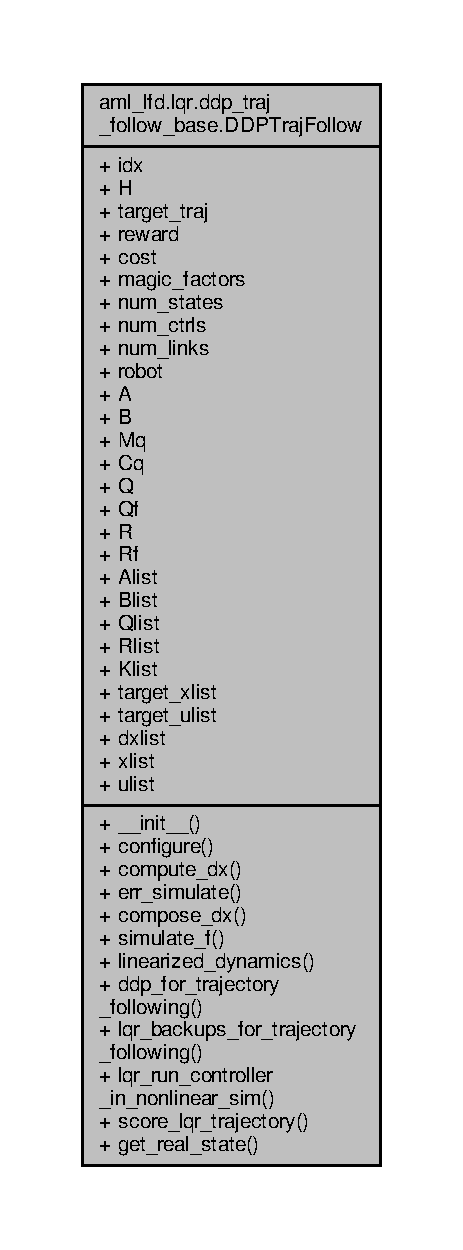
\includegraphics[height=550pt]{classaml__lfd_1_1lqr_1_1ddp__traj__follow__base_1_1_d_d_p_traj_follow__coll__graph}
\end{center}
\end{figure}
\subsection*{Public Member Functions}
\begin{DoxyCompactItemize}
\item 
\hypertarget{classaml__lfd_1_1lqr_1_1ddp__traj__follow__base_1_1_d_d_p_traj_follow_a056ad6c1307488c0ce377da8e5cf8bdb}{def {\bfseries \-\_\-\-\_\-init\-\_\-\-\_\-}}\label{classaml__lfd_1_1lqr_1_1ddp__traj__follow__base_1_1_d_d_p_traj_follow_a056ad6c1307488c0ce377da8e5cf8bdb}

\item 
\hypertarget{classaml__lfd_1_1lqr_1_1ddp__traj__follow__base_1_1_d_d_p_traj_follow_a90408dc24bbe915a9e95a87f1cc21d7d}{def {\bfseries configure}}\label{classaml__lfd_1_1lqr_1_1ddp__traj__follow__base_1_1_d_d_p_traj_follow_a90408dc24bbe915a9e95a87f1cc21d7d}

\item 
\hypertarget{classaml__lfd_1_1lqr_1_1ddp__traj__follow__base_1_1_d_d_p_traj_follow_a16dd3bb218fb2a761dedba0077ea5c75}{def {\bfseries compute\-\_\-dx}}\label{classaml__lfd_1_1lqr_1_1ddp__traj__follow__base_1_1_d_d_p_traj_follow_a16dd3bb218fb2a761dedba0077ea5c75}

\item 
\hypertarget{classaml__lfd_1_1lqr_1_1ddp__traj__follow__base_1_1_d_d_p_traj_follow_a29454de12b3272d19d31f1b9763a8c84}{def {\bfseries err\-\_\-simulate}}\label{classaml__lfd_1_1lqr_1_1ddp__traj__follow__base_1_1_d_d_p_traj_follow_a29454de12b3272d19d31f1b9763a8c84}

\item 
\hypertarget{classaml__lfd_1_1lqr_1_1ddp__traj__follow__base_1_1_d_d_p_traj_follow_a8aeae647129bd99e45a5601eaffa6ae9}{def {\bfseries compose\-\_\-dx}}\label{classaml__lfd_1_1lqr_1_1ddp__traj__follow__base_1_1_d_d_p_traj_follow_a8aeae647129bd99e45a5601eaffa6ae9}

\item 
\hypertarget{classaml__lfd_1_1lqr_1_1ddp__traj__follow__base_1_1_d_d_p_traj_follow_af7d1f720102dc0a16ab0e0259fee6bd4}{def {\bfseries simulate\-\_\-f}}\label{classaml__lfd_1_1lqr_1_1ddp__traj__follow__base_1_1_d_d_p_traj_follow_af7d1f720102dc0a16ab0e0259fee6bd4}

\item 
\hypertarget{classaml__lfd_1_1lqr_1_1ddp__traj__follow__base_1_1_d_d_p_traj_follow_ad99452c989bdd3f69793bf9d47060aab}{def {\bfseries linearized\-\_\-dynamics}}\label{classaml__lfd_1_1lqr_1_1ddp__traj__follow__base_1_1_d_d_p_traj_follow_ad99452c989bdd3f69793bf9d47060aab}

\item 
\hypertarget{classaml__lfd_1_1lqr_1_1ddp__traj__follow__base_1_1_d_d_p_traj_follow_adbd0641ee97f6f570336cba071f2e491}{def {\bfseries ddp\-\_\-for\-\_\-trajectory\-\_\-following}}\label{classaml__lfd_1_1lqr_1_1ddp__traj__follow__base_1_1_d_d_p_traj_follow_adbd0641ee97f6f570336cba071f2e491}

\item 
\hypertarget{classaml__lfd_1_1lqr_1_1ddp__traj__follow__base_1_1_d_d_p_traj_follow_a1d87e2ffffb673f72cf13b55c6d81846}{def {\bfseries lqr\-\_\-backups\-\_\-for\-\_\-trajectory\-\_\-following}}\label{classaml__lfd_1_1lqr_1_1ddp__traj__follow__base_1_1_d_d_p_traj_follow_a1d87e2ffffb673f72cf13b55c6d81846}

\item 
\hypertarget{classaml__lfd_1_1lqr_1_1ddp__traj__follow__base_1_1_d_d_p_traj_follow_aece8a96b5eb3535ef06ebc70a248eea9}{def {\bfseries lqr\-\_\-run\-\_\-controller\-\_\-in\-\_\-nonlinear\-\_\-sim}}\label{classaml__lfd_1_1lqr_1_1ddp__traj__follow__base_1_1_d_d_p_traj_follow_aece8a96b5eb3535ef06ebc70a248eea9}

\item 
\hypertarget{classaml__lfd_1_1lqr_1_1ddp__traj__follow__base_1_1_d_d_p_traj_follow_a21f0b4c8898671073bd6cdd2c8347e29}{def {\bfseries score\-\_\-lqr\-\_\-trajectory}}\label{classaml__lfd_1_1lqr_1_1ddp__traj__follow__base_1_1_d_d_p_traj_follow_a21f0b4c8898671073bd6cdd2c8347e29}

\item 
\hypertarget{classaml__lfd_1_1lqr_1_1ddp__traj__follow__base_1_1_d_d_p_traj_follow_ab064db58d2709906da9fdb29aee40a93}{def {\bfseries get\-\_\-real\-\_\-state}}\label{classaml__lfd_1_1lqr_1_1ddp__traj__follow__base_1_1_d_d_p_traj_follow_ab064db58d2709906da9fdb29aee40a93}

\end{DoxyCompactItemize}
\subsection*{Public Attributes}
\begin{DoxyCompactItemize}
\item 
\hypertarget{classaml__lfd_1_1lqr_1_1ddp__traj__follow__base_1_1_d_d_p_traj_follow_af0b6fbbc185f857a746ca2981001e4fa}{{\bfseries idx}}\label{classaml__lfd_1_1lqr_1_1ddp__traj__follow__base_1_1_d_d_p_traj_follow_af0b6fbbc185f857a746ca2981001e4fa}

\item 
\hypertarget{classaml__lfd_1_1lqr_1_1ddp__traj__follow__base_1_1_d_d_p_traj_follow_aec1df18773cc7d2f37d95e9408d4748f}{{\bfseries H}}\label{classaml__lfd_1_1lqr_1_1ddp__traj__follow__base_1_1_d_d_p_traj_follow_aec1df18773cc7d2f37d95e9408d4748f}

\item 
\hypertarget{classaml__lfd_1_1lqr_1_1ddp__traj__follow__base_1_1_d_d_p_traj_follow_a03f52d1545917a8954bd837c9fc428f8}{{\bfseries target\-\_\-traj}}\label{classaml__lfd_1_1lqr_1_1ddp__traj__follow__base_1_1_d_d_p_traj_follow_a03f52d1545917a8954bd837c9fc428f8}

\item 
\hypertarget{classaml__lfd_1_1lqr_1_1ddp__traj__follow__base_1_1_d_d_p_traj_follow_a1f8edf414c5f464fca690964c2a9bf7a}{{\bfseries reward}}\label{classaml__lfd_1_1lqr_1_1ddp__traj__follow__base_1_1_d_d_p_traj_follow_a1f8edf414c5f464fca690964c2a9bf7a}

\item 
\hypertarget{classaml__lfd_1_1lqr_1_1ddp__traj__follow__base_1_1_d_d_p_traj_follow_a843d69188b565822569099d0832f2b60}{{\bfseries cost}}\label{classaml__lfd_1_1lqr_1_1ddp__traj__follow__base_1_1_d_d_p_traj_follow_a843d69188b565822569099d0832f2b60}

\item 
\hypertarget{classaml__lfd_1_1lqr_1_1ddp__traj__follow__base_1_1_d_d_p_traj_follow_a76562065147ed65895d58af5f78b9e3b}{{\bfseries magic\-\_\-factors}}\label{classaml__lfd_1_1lqr_1_1ddp__traj__follow__base_1_1_d_d_p_traj_follow_a76562065147ed65895d58af5f78b9e3b}

\item 
\hypertarget{classaml__lfd_1_1lqr_1_1ddp__traj__follow__base_1_1_d_d_p_traj_follow_a3ff02e2708357534cb2af0d8a7e5560d}{{\bfseries num\-\_\-states}}\label{classaml__lfd_1_1lqr_1_1ddp__traj__follow__base_1_1_d_d_p_traj_follow_a3ff02e2708357534cb2af0d8a7e5560d}

\item 
\hypertarget{classaml__lfd_1_1lqr_1_1ddp__traj__follow__base_1_1_d_d_p_traj_follow_ac565b2592399d6c46eaa9603649e8bd1}{{\bfseries num\-\_\-ctrls}}\label{classaml__lfd_1_1lqr_1_1ddp__traj__follow__base_1_1_d_d_p_traj_follow_ac565b2592399d6c46eaa9603649e8bd1}

\item 
\hypertarget{classaml__lfd_1_1lqr_1_1ddp__traj__follow__base_1_1_d_d_p_traj_follow_a4cfe2bc27d78ce4dd4f96f591e812386}{{\bfseries num\-\_\-links}}\label{classaml__lfd_1_1lqr_1_1ddp__traj__follow__base_1_1_d_d_p_traj_follow_a4cfe2bc27d78ce4dd4f96f591e812386}

\item 
\hypertarget{classaml__lfd_1_1lqr_1_1ddp__traj__follow__base_1_1_d_d_p_traj_follow_a9bc25164edb2c2e29743ed1a8eb64488}{{\bfseries robot}}\label{classaml__lfd_1_1lqr_1_1ddp__traj__follow__base_1_1_d_d_p_traj_follow_a9bc25164edb2c2e29743ed1a8eb64488}

\item 
\hypertarget{classaml__lfd_1_1lqr_1_1ddp__traj__follow__base_1_1_d_d_p_traj_follow_ad7d04202fc2d76e5a955e5ffb71633cd}{{\bfseries A}}\label{classaml__lfd_1_1lqr_1_1ddp__traj__follow__base_1_1_d_d_p_traj_follow_ad7d04202fc2d76e5a955e5ffb71633cd}

\item 
\hypertarget{classaml__lfd_1_1lqr_1_1ddp__traj__follow__base_1_1_d_d_p_traj_follow_a63516b4578bc9ae85b609c7b1d8cc8db}{{\bfseries B}}\label{classaml__lfd_1_1lqr_1_1ddp__traj__follow__base_1_1_d_d_p_traj_follow_a63516b4578bc9ae85b609c7b1d8cc8db}

\item 
\hypertarget{classaml__lfd_1_1lqr_1_1ddp__traj__follow__base_1_1_d_d_p_traj_follow_a2dd2df27d2b4ea3cd0a91db3fda4427a}{{\bfseries Mq}}\label{classaml__lfd_1_1lqr_1_1ddp__traj__follow__base_1_1_d_d_p_traj_follow_a2dd2df27d2b4ea3cd0a91db3fda4427a}

\item 
\hypertarget{classaml__lfd_1_1lqr_1_1ddp__traj__follow__base_1_1_d_d_p_traj_follow_a0b0e42bc2ff3b66681542f8d8c38e100}{{\bfseries Cq}}\label{classaml__lfd_1_1lqr_1_1ddp__traj__follow__base_1_1_d_d_p_traj_follow_a0b0e42bc2ff3b66681542f8d8c38e100}

\item 
\hypertarget{classaml__lfd_1_1lqr_1_1ddp__traj__follow__base_1_1_d_d_p_traj_follow_a1173c1b05d86aa568abcab18b7bd69ea}{{\bfseries Q}}\label{classaml__lfd_1_1lqr_1_1ddp__traj__follow__base_1_1_d_d_p_traj_follow_a1173c1b05d86aa568abcab18b7bd69ea}

\item 
\hypertarget{classaml__lfd_1_1lqr_1_1ddp__traj__follow__base_1_1_d_d_p_traj_follow_abf905d9982f96f9ed454961c42359f9f}{{\bfseries Qf}}\label{classaml__lfd_1_1lqr_1_1ddp__traj__follow__base_1_1_d_d_p_traj_follow_abf905d9982f96f9ed454961c42359f9f}

\item 
\hypertarget{classaml__lfd_1_1lqr_1_1ddp__traj__follow__base_1_1_d_d_p_traj_follow_a70e3c8b1d5e33f94e5141075ebf02975}{{\bfseries R}}\label{classaml__lfd_1_1lqr_1_1ddp__traj__follow__base_1_1_d_d_p_traj_follow_a70e3c8b1d5e33f94e5141075ebf02975}

\item 
\hypertarget{classaml__lfd_1_1lqr_1_1ddp__traj__follow__base_1_1_d_d_p_traj_follow_a6c6bfb30d6a4c345412210240fb0e296}{{\bfseries Rf}}\label{classaml__lfd_1_1lqr_1_1ddp__traj__follow__base_1_1_d_d_p_traj_follow_a6c6bfb30d6a4c345412210240fb0e296}

\item 
\hypertarget{classaml__lfd_1_1lqr_1_1ddp__traj__follow__base_1_1_d_d_p_traj_follow_a577e00ce473a24465c4f0de0a146ef3e}{{\bfseries Alist}}\label{classaml__lfd_1_1lqr_1_1ddp__traj__follow__base_1_1_d_d_p_traj_follow_a577e00ce473a24465c4f0de0a146ef3e}

\item 
\hypertarget{classaml__lfd_1_1lqr_1_1ddp__traj__follow__base_1_1_d_d_p_traj_follow_a5da728040bfb20c0144f91e4e3f8cb36}{{\bfseries Blist}}\label{classaml__lfd_1_1lqr_1_1ddp__traj__follow__base_1_1_d_d_p_traj_follow_a5da728040bfb20c0144f91e4e3f8cb36}

\item 
\hypertarget{classaml__lfd_1_1lqr_1_1ddp__traj__follow__base_1_1_d_d_p_traj_follow_aeee69abfc8dd387e0ef2b752be44f2f6}{{\bfseries Qlist}}\label{classaml__lfd_1_1lqr_1_1ddp__traj__follow__base_1_1_d_d_p_traj_follow_aeee69abfc8dd387e0ef2b752be44f2f6}

\item 
\hypertarget{classaml__lfd_1_1lqr_1_1ddp__traj__follow__base_1_1_d_d_p_traj_follow_ae4c9a614b6a275e49e6f39bcb76b27b6}{{\bfseries Rlist}}\label{classaml__lfd_1_1lqr_1_1ddp__traj__follow__base_1_1_d_d_p_traj_follow_ae4c9a614b6a275e49e6f39bcb76b27b6}

\item 
\hypertarget{classaml__lfd_1_1lqr_1_1ddp__traj__follow__base_1_1_d_d_p_traj_follow_a1fc53a0218dd657abe54fa4585c35cd1}{{\bfseries Klist}}\label{classaml__lfd_1_1lqr_1_1ddp__traj__follow__base_1_1_d_d_p_traj_follow_a1fc53a0218dd657abe54fa4585c35cd1}

\item 
\hypertarget{classaml__lfd_1_1lqr_1_1ddp__traj__follow__base_1_1_d_d_p_traj_follow_ac8045400042e1740c62cd987a5bd78be}{{\bfseries target\-\_\-xlist}}\label{classaml__lfd_1_1lqr_1_1ddp__traj__follow__base_1_1_d_d_p_traj_follow_ac8045400042e1740c62cd987a5bd78be}

\item 
\hypertarget{classaml__lfd_1_1lqr_1_1ddp__traj__follow__base_1_1_d_d_p_traj_follow_af8fb8b26f0014cc318a822a1ecce6859}{{\bfseries target\-\_\-ulist}}\label{classaml__lfd_1_1lqr_1_1ddp__traj__follow__base_1_1_d_d_p_traj_follow_af8fb8b26f0014cc318a822a1ecce6859}

\item 
\hypertarget{classaml__lfd_1_1lqr_1_1ddp__traj__follow__base_1_1_d_d_p_traj_follow_a6d2157818c66fe4ca6c57414262309a4}{{\bfseries dxlist}}\label{classaml__lfd_1_1lqr_1_1ddp__traj__follow__base_1_1_d_d_p_traj_follow_a6d2157818c66fe4ca6c57414262309a4}

\item 
\hypertarget{classaml__lfd_1_1lqr_1_1ddp__traj__follow__base_1_1_d_d_p_traj_follow_a737296883bc4be3b617e584833125ed3}{{\bfseries xlist}}\label{classaml__lfd_1_1lqr_1_1ddp__traj__follow__base_1_1_d_d_p_traj_follow_a737296883bc4be3b617e584833125ed3}

\item 
\hypertarget{classaml__lfd_1_1lqr_1_1ddp__traj__follow__base_1_1_d_d_p_traj_follow_a23c501383ace126e72954a4e9e3138f1}{{\bfseries ulist}}\label{classaml__lfd_1_1lqr_1_1ddp__traj__follow__base_1_1_d_d_p_traj_follow_a23c501383ace126e72954a4e9e3138f1}

\end{DoxyCompactItemize}


The documentation for this class was generated from the following file\-:\begin{DoxyCompactItemize}
\item 
aml\-\_\-lfd/src/aml\-\_\-lfd/lqr/ddp\-\_\-traj\-\_\-follow\-\_\-base.\-py\end{DoxyCompactItemize}

\hypertarget{classaml__lfd_1_1dmp_1_1discrete__dmp__shell_1_1_discrete_d_m_p_shell}{}\section{aml\+\_\+lfd.\+dmp.\+discrete\+\_\+dmp\+\_\+shell.\+Discrete\+D\+M\+P\+Shell Class Reference}
\label{classaml__lfd_1_1dmp_1_1discrete__dmp__shell_1_1_discrete_d_m_p_shell}\index{aml\+\_\+lfd.\+dmp.\+discrete\+\_\+dmp\+\_\+shell.\+Discrete\+D\+M\+P\+Shell@{aml\+\_\+lfd.\+dmp.\+discrete\+\_\+dmp\+\_\+shell.\+Discrete\+D\+M\+P\+Shell}}


Inheritance diagram for aml\+\_\+lfd.\+dmp.\+discrete\+\_\+dmp\+\_\+shell.\+Discrete\+D\+M\+P\+Shell\+:\nopagebreak
\begin{figure}[H]
\begin{center}
\leavevmode
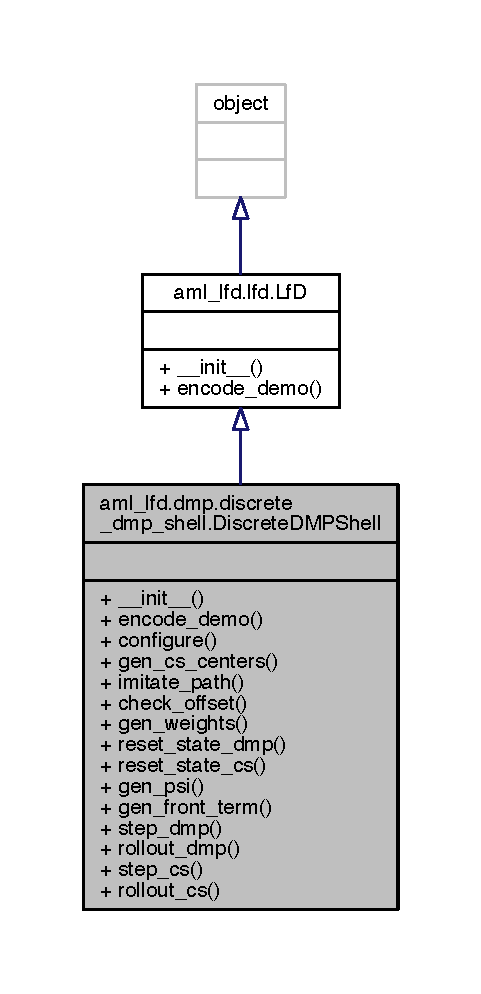
\includegraphics[width=231pt]{classaml__lfd_1_1dmp_1_1discrete__dmp__shell_1_1_discrete_d_m_p_shell__inherit__graph}
\end{center}
\end{figure}


Collaboration diagram for aml\+\_\+lfd.\+dmp.\+discrete\+\_\+dmp\+\_\+shell.\+Discrete\+D\+M\+P\+Shell\+:\nopagebreak
\begin{figure}[H]
\begin{center}
\leavevmode
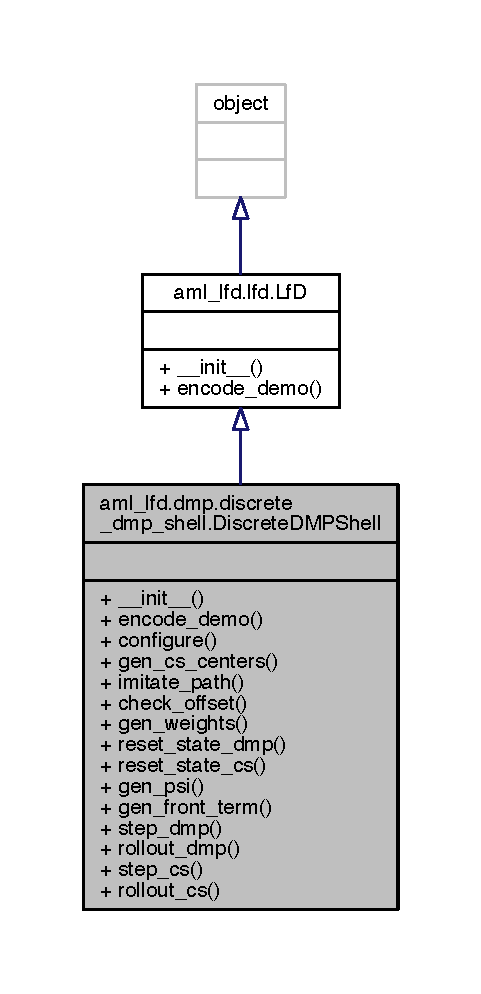
\includegraphics[width=231pt]{classaml__lfd_1_1dmp_1_1discrete__dmp__shell_1_1_discrete_d_m_p_shell__coll__graph}
\end{center}
\end{figure}
\subsection*{Public Member Functions}
\begin{DoxyCompactItemize}
\item 
\hypertarget{classaml__lfd_1_1dmp_1_1discrete__dmp__shell_1_1_discrete_d_m_p_shell_afdc79719c645bf1ffd4166faff1ce082}{}\label{classaml__lfd_1_1dmp_1_1discrete__dmp__shell_1_1_discrete_d_m_p_shell_afdc79719c645bf1ffd4166faff1ce082} 
def {\bfseries \+\_\+\+\_\+init\+\_\+\+\_\+} (self, config=D\+I\+S\+C\+R\+E\+T\+E\+\_\+\+D\+MP)
\item 
\hypertarget{classaml__lfd_1_1dmp_1_1discrete__dmp__shell_1_1_discrete_d_m_p_shell_a8e9bcf0d7885c2b6e8bef7b57ea3ffbe}{}\label{classaml__lfd_1_1dmp_1_1discrete__dmp__shell_1_1_discrete_d_m_p_shell_a8e9bcf0d7885c2b6e8bef7b57ea3ffbe} 
def {\bfseries encode\+\_\+demo} (self)
\item 
\hypertarget{classaml__lfd_1_1dmp_1_1discrete__dmp__shell_1_1_discrete_d_m_p_shell_a5d15a53724bb01efe93bc3a176837458}{}\label{classaml__lfd_1_1dmp_1_1discrete__dmp__shell_1_1_discrete_d_m_p_shell_a5d15a53724bb01efe93bc3a176837458} 
def {\bfseries configure} (self, traj2follow, start, goal)
\item 
def \hyperlink{classaml__lfd_1_1dmp_1_1discrete__dmp__shell_1_1_discrete_d_m_p_shell_ab364e2625c5983ba748c212e7cc4b16b}{gen\+\_\+cs\+\_\+centers} (self)
\item 
def \hyperlink{classaml__lfd_1_1dmp_1_1discrete__dmp__shell_1_1_discrete_d_m_p_shell_a2036e592bfd791bf24f238f9636b42ff}{imitate\+\_\+path} (self)
\item 
def \hyperlink{classaml__lfd_1_1dmp_1_1discrete__dmp__shell_1_1_discrete_d_m_p_shell_a10cec75150acb1c2e426fc17ce22bde6}{check\+\_\+offset} (self)
\item 
def \hyperlink{classaml__lfd_1_1dmp_1_1discrete__dmp__shell_1_1_discrete_d_m_p_shell_a369eaa244df73de31517906315c98772}{gen\+\_\+weights} (self, f\+\_\+target)
\item 
def \hyperlink{classaml__lfd_1_1dmp_1_1discrete__dmp__shell_1_1_discrete_d_m_p_shell_a07482e8fe6955be1c72e67258953e298}{reset\+\_\+state\+\_\+dmp} (self, new\+\_\+start=None)
\item 
def \hyperlink{classaml__lfd_1_1dmp_1_1discrete__dmp__shell_1_1_discrete_d_m_p_shell_a26c7a072996b7b5e2cdb13f19e3c3053}{reset\+\_\+state\+\_\+cs} (self)
\item 
def \hyperlink{classaml__lfd_1_1dmp_1_1discrete__dmp__shell_1_1_discrete_d_m_p_shell_a0da4fbcdb74db7ca2d32e5913be72a81}{gen\+\_\+psi} (self, x)
\item 
def \hyperlink{classaml__lfd_1_1dmp_1_1discrete__dmp__shell_1_1_discrete_d_m_p_shell_a49cf27ca02e86e1773133835e1f606a2}{gen\+\_\+front\+\_\+term} (self, x, dmp\+\_\+num)
\item 
def \hyperlink{classaml__lfd_1_1dmp_1_1discrete__dmp__shell_1_1_discrete_d_m_p_shell_a198fd652ccf7f3d54a77361f521ca3ae}{step\+\_\+dmp} (self, tau=None, state\+\_\+fb=None, external\+\_\+force=None)
\item 
def \hyperlink{classaml__lfd_1_1dmp_1_1discrete__dmp__shell_1_1_discrete_d_m_p_shell_ad46fa7e783a6c38e19bb6f36fed76a8b}{rollout\+\_\+dmp} (self, tau=None)
\item 
def \hyperlink{classaml__lfd_1_1dmp_1_1discrete__dmp__shell_1_1_discrete_d_m_p_shell_aeff4509250d19885d751a439f3eff8f5}{step\+\_\+cs} (self, tau=1.\+0, error\+\_\+coupling=1.\+0)
\item 
def \hyperlink{classaml__lfd_1_1dmp_1_1discrete__dmp__shell_1_1_discrete_d_m_p_shell_a21a2c8cac5774e8dbd87a211fda6ef05}{rollout\+\_\+cs} (self, kwargs)
\end{DoxyCompactItemize}


\subsection{Member Function Documentation}
\hypertarget{classaml__lfd_1_1dmp_1_1discrete__dmp__shell_1_1_discrete_d_m_p_shell_a10cec75150acb1c2e426fc17ce22bde6}{}\label{classaml__lfd_1_1dmp_1_1discrete__dmp__shell_1_1_discrete_d_m_p_shell_a10cec75150acb1c2e426fc17ce22bde6} 
\index{aml\+\_\+lfd\+::dmp\+::discrete\+\_\+dmp\+\_\+shell\+::\+Discrete\+D\+M\+P\+Shell@{aml\+\_\+lfd\+::dmp\+::discrete\+\_\+dmp\+\_\+shell\+::\+Discrete\+D\+M\+P\+Shell}!check\+\_\+offset@{check\+\_\+offset}}
\index{check\+\_\+offset@{check\+\_\+offset}!aml\+\_\+lfd\+::dmp\+::discrete\+\_\+dmp\+\_\+shell\+::\+Discrete\+D\+M\+P\+Shell@{aml\+\_\+lfd\+::dmp\+::discrete\+\_\+dmp\+\_\+shell\+::\+Discrete\+D\+M\+P\+Shell}}
\subsubsection{\texorpdfstring{check\+\_\+offset()}{check\_offset()}}
{\footnotesize\ttfamily def aml\+\_\+lfd.\+dmp.\+discrete\+\_\+dmp\+\_\+shell.\+Discrete\+D\+M\+P\+Shell.\+check\+\_\+offset (\begin{DoxyParamCaption}\item[{}]{self }\end{DoxyParamCaption})}

\begin{DoxyVerb}Check to see if initial position and goal are the same
if they are, offset slightly so that the forcing term is not 0\end{DoxyVerb}
 \hypertarget{classaml__lfd_1_1dmp_1_1discrete__dmp__shell_1_1_discrete_d_m_p_shell_ab364e2625c5983ba748c212e7cc4b16b}{}\label{classaml__lfd_1_1dmp_1_1discrete__dmp__shell_1_1_discrete_d_m_p_shell_ab364e2625c5983ba748c212e7cc4b16b} 
\index{aml\+\_\+lfd\+::dmp\+::discrete\+\_\+dmp\+\_\+shell\+::\+Discrete\+D\+M\+P\+Shell@{aml\+\_\+lfd\+::dmp\+::discrete\+\_\+dmp\+\_\+shell\+::\+Discrete\+D\+M\+P\+Shell}!gen\+\_\+cs\+\_\+centers@{gen\+\_\+cs\+\_\+centers}}
\index{gen\+\_\+cs\+\_\+centers@{gen\+\_\+cs\+\_\+centers}!aml\+\_\+lfd\+::dmp\+::discrete\+\_\+dmp\+\_\+shell\+::\+Discrete\+D\+M\+P\+Shell@{aml\+\_\+lfd\+::dmp\+::discrete\+\_\+dmp\+\_\+shell\+::\+Discrete\+D\+M\+P\+Shell}}
\subsubsection{\texorpdfstring{gen\+\_\+cs\+\_\+centers()}{gen\_cs\_centers()}}
{\footnotesize\ttfamily def aml\+\_\+lfd.\+dmp.\+discrete\+\_\+dmp\+\_\+shell.\+Discrete\+D\+M\+P\+Shell.\+gen\+\_\+cs\+\_\+centers (\begin{DoxyParamCaption}\item[{}]{self }\end{DoxyParamCaption})}

\begin{DoxyVerb}Set the centre of the Gaussian basis 
functions be spaced evenly throughout run time\end{DoxyVerb}
 \hypertarget{classaml__lfd_1_1dmp_1_1discrete__dmp__shell_1_1_discrete_d_m_p_shell_a49cf27ca02e86e1773133835e1f606a2}{}\label{classaml__lfd_1_1dmp_1_1discrete__dmp__shell_1_1_discrete_d_m_p_shell_a49cf27ca02e86e1773133835e1f606a2} 
\index{aml\+\_\+lfd\+::dmp\+::discrete\+\_\+dmp\+\_\+shell\+::\+Discrete\+D\+M\+P\+Shell@{aml\+\_\+lfd\+::dmp\+::discrete\+\_\+dmp\+\_\+shell\+::\+Discrete\+D\+M\+P\+Shell}!gen\+\_\+front\+\_\+term@{gen\+\_\+front\+\_\+term}}
\index{gen\+\_\+front\+\_\+term@{gen\+\_\+front\+\_\+term}!aml\+\_\+lfd\+::dmp\+::discrete\+\_\+dmp\+\_\+shell\+::\+Discrete\+D\+M\+P\+Shell@{aml\+\_\+lfd\+::dmp\+::discrete\+\_\+dmp\+\_\+shell\+::\+Discrete\+D\+M\+P\+Shell}}
\subsubsection{\texorpdfstring{gen\+\_\+front\+\_\+term()}{gen\_front\_term()}}
{\footnotesize\ttfamily def aml\+\_\+lfd.\+dmp.\+discrete\+\_\+dmp\+\_\+shell.\+Discrete\+D\+M\+P\+Shell.\+gen\+\_\+front\+\_\+term (\begin{DoxyParamCaption}\item[{}]{self,  }\item[{}]{x,  }\item[{}]{dmp\+\_\+num }\end{DoxyParamCaption})}

\begin{DoxyVerb}Generates the diminishing front term on 
the forcing term.

x float: the current value of the canonical system
dmp_num int: the index of the current dmp
\end{DoxyVerb}
 \hypertarget{classaml__lfd_1_1dmp_1_1discrete__dmp__shell_1_1_discrete_d_m_p_shell_a0da4fbcdb74db7ca2d32e5913be72a81}{}\label{classaml__lfd_1_1dmp_1_1discrete__dmp__shell_1_1_discrete_d_m_p_shell_a0da4fbcdb74db7ca2d32e5913be72a81} 
\index{aml\+\_\+lfd\+::dmp\+::discrete\+\_\+dmp\+\_\+shell\+::\+Discrete\+D\+M\+P\+Shell@{aml\+\_\+lfd\+::dmp\+::discrete\+\_\+dmp\+\_\+shell\+::\+Discrete\+D\+M\+P\+Shell}!gen\+\_\+psi@{gen\+\_\+psi}}
\index{gen\+\_\+psi@{gen\+\_\+psi}!aml\+\_\+lfd\+::dmp\+::discrete\+\_\+dmp\+\_\+shell\+::\+Discrete\+D\+M\+P\+Shell@{aml\+\_\+lfd\+::dmp\+::discrete\+\_\+dmp\+\_\+shell\+::\+Discrete\+D\+M\+P\+Shell}}
\subsubsection{\texorpdfstring{gen\+\_\+psi()}{gen\_psi()}}
{\footnotesize\ttfamily def aml\+\_\+lfd.\+dmp.\+discrete\+\_\+dmp\+\_\+shell.\+Discrete\+D\+M\+P\+Shell.\+gen\+\_\+psi (\begin{DoxyParamCaption}\item[{}]{self,  }\item[{}]{x }\end{DoxyParamCaption})}

\begin{DoxyVerb}Generates the activity of the basis functions for a given 
canonical system rollout. 

x float, array: the canonical system state or path
\end{DoxyVerb}
 \hypertarget{classaml__lfd_1_1dmp_1_1discrete__dmp__shell_1_1_discrete_d_m_p_shell_a369eaa244df73de31517906315c98772}{}\label{classaml__lfd_1_1dmp_1_1discrete__dmp__shell_1_1_discrete_d_m_p_shell_a369eaa244df73de31517906315c98772} 
\index{aml\+\_\+lfd\+::dmp\+::discrete\+\_\+dmp\+\_\+shell\+::\+Discrete\+D\+M\+P\+Shell@{aml\+\_\+lfd\+::dmp\+::discrete\+\_\+dmp\+\_\+shell\+::\+Discrete\+D\+M\+P\+Shell}!gen\+\_\+weights@{gen\+\_\+weights}}
\index{gen\+\_\+weights@{gen\+\_\+weights}!aml\+\_\+lfd\+::dmp\+::discrete\+\_\+dmp\+\_\+shell\+::\+Discrete\+D\+M\+P\+Shell@{aml\+\_\+lfd\+::dmp\+::discrete\+\_\+dmp\+\_\+shell\+::\+Discrete\+D\+M\+P\+Shell}}
\subsubsection{\texorpdfstring{gen\+\_\+weights()}{gen\_weights()}}
{\footnotesize\ttfamily def aml\+\_\+lfd.\+dmp.\+discrete\+\_\+dmp\+\_\+shell.\+Discrete\+D\+M\+P\+Shell.\+gen\+\_\+weights (\begin{DoxyParamCaption}\item[{}]{self,  }\item[{}]{f\+\_\+target }\end{DoxyParamCaption})}

\begin{DoxyVerb}Generate a set of weights over the basis functions such 
that the target forcing term trajectory is matched.

f_target np.array: the desired forcing term trajectory
\end{DoxyVerb}
 \hypertarget{classaml__lfd_1_1dmp_1_1discrete__dmp__shell_1_1_discrete_d_m_p_shell_a2036e592bfd791bf24f238f9636b42ff}{}\label{classaml__lfd_1_1dmp_1_1discrete__dmp__shell_1_1_discrete_d_m_p_shell_a2036e592bfd791bf24f238f9636b42ff} 
\index{aml\+\_\+lfd\+::dmp\+::discrete\+\_\+dmp\+\_\+shell\+::\+Discrete\+D\+M\+P\+Shell@{aml\+\_\+lfd\+::dmp\+::discrete\+\_\+dmp\+\_\+shell\+::\+Discrete\+D\+M\+P\+Shell}!imitate\+\_\+path@{imitate\+\_\+path}}
\index{imitate\+\_\+path@{imitate\+\_\+path}!aml\+\_\+lfd\+::dmp\+::discrete\+\_\+dmp\+\_\+shell\+::\+Discrete\+D\+M\+P\+Shell@{aml\+\_\+lfd\+::dmp\+::discrete\+\_\+dmp\+\_\+shell\+::\+Discrete\+D\+M\+P\+Shell}}
\subsubsection{\texorpdfstring{imitate\+\_\+path()}{imitate\_path()}}
{\footnotesize\ttfamily def aml\+\_\+lfd.\+dmp.\+discrete\+\_\+dmp\+\_\+shell.\+Discrete\+D\+M\+P\+Shell.\+imitate\+\_\+path (\begin{DoxyParamCaption}\item[{}]{self }\end{DoxyParamCaption})}

\begin{DoxyVerb}Takes in a desired trajectory and generates the set of 
system parameters that best realize this path.
    
y_des list/array: the desired trajectories of each DMP
          should be shaped [dmps, run_time]
\end{DoxyVerb}
 \hypertarget{classaml__lfd_1_1dmp_1_1discrete__dmp__shell_1_1_discrete_d_m_p_shell_a26c7a072996b7b5e2cdb13f19e3c3053}{}\label{classaml__lfd_1_1dmp_1_1discrete__dmp__shell_1_1_discrete_d_m_p_shell_a26c7a072996b7b5e2cdb13f19e3c3053} 
\index{aml\+\_\+lfd\+::dmp\+::discrete\+\_\+dmp\+\_\+shell\+::\+Discrete\+D\+M\+P\+Shell@{aml\+\_\+lfd\+::dmp\+::discrete\+\_\+dmp\+\_\+shell\+::\+Discrete\+D\+M\+P\+Shell}!reset\+\_\+state\+\_\+cs@{reset\+\_\+state\+\_\+cs}}
\index{reset\+\_\+state\+\_\+cs@{reset\+\_\+state\+\_\+cs}!aml\+\_\+lfd\+::dmp\+::discrete\+\_\+dmp\+\_\+shell\+::\+Discrete\+D\+M\+P\+Shell@{aml\+\_\+lfd\+::dmp\+::discrete\+\_\+dmp\+\_\+shell\+::\+Discrete\+D\+M\+P\+Shell}}
\subsubsection{\texorpdfstring{reset\+\_\+state\+\_\+cs()}{reset\_state\_cs()}}
{\footnotesize\ttfamily def aml\+\_\+lfd.\+dmp.\+discrete\+\_\+dmp\+\_\+shell.\+Discrete\+D\+M\+P\+Shell.\+reset\+\_\+state\+\_\+cs (\begin{DoxyParamCaption}\item[{}]{self }\end{DoxyParamCaption})}

\begin{DoxyVerb}Reset the system state\end{DoxyVerb}
 \hypertarget{classaml__lfd_1_1dmp_1_1discrete__dmp__shell_1_1_discrete_d_m_p_shell_a07482e8fe6955be1c72e67258953e298}{}\label{classaml__lfd_1_1dmp_1_1discrete__dmp__shell_1_1_discrete_d_m_p_shell_a07482e8fe6955be1c72e67258953e298} 
\index{aml\+\_\+lfd\+::dmp\+::discrete\+\_\+dmp\+\_\+shell\+::\+Discrete\+D\+M\+P\+Shell@{aml\+\_\+lfd\+::dmp\+::discrete\+\_\+dmp\+\_\+shell\+::\+Discrete\+D\+M\+P\+Shell}!reset\+\_\+state\+\_\+dmp@{reset\+\_\+state\+\_\+dmp}}
\index{reset\+\_\+state\+\_\+dmp@{reset\+\_\+state\+\_\+dmp}!aml\+\_\+lfd\+::dmp\+::discrete\+\_\+dmp\+\_\+shell\+::\+Discrete\+D\+M\+P\+Shell@{aml\+\_\+lfd\+::dmp\+::discrete\+\_\+dmp\+\_\+shell\+::\+Discrete\+D\+M\+P\+Shell}}
\subsubsection{\texorpdfstring{reset\+\_\+state\+\_\+dmp()}{reset\_state\_dmp()}}
{\footnotesize\ttfamily def aml\+\_\+lfd.\+dmp.\+discrete\+\_\+dmp\+\_\+shell.\+Discrete\+D\+M\+P\+Shell.\+reset\+\_\+state\+\_\+dmp (\begin{DoxyParamCaption}\item[{}]{self,  }\item[{}]{new\+\_\+start = {\ttfamily None} }\end{DoxyParamCaption})}

\begin{DoxyVerb}Reset the system state\end{DoxyVerb}
 \hypertarget{classaml__lfd_1_1dmp_1_1discrete__dmp__shell_1_1_discrete_d_m_p_shell_a21a2c8cac5774e8dbd87a211fda6ef05}{}\label{classaml__lfd_1_1dmp_1_1discrete__dmp__shell_1_1_discrete_d_m_p_shell_a21a2c8cac5774e8dbd87a211fda6ef05} 
\index{aml\+\_\+lfd\+::dmp\+::discrete\+\_\+dmp\+\_\+shell\+::\+Discrete\+D\+M\+P\+Shell@{aml\+\_\+lfd\+::dmp\+::discrete\+\_\+dmp\+\_\+shell\+::\+Discrete\+D\+M\+P\+Shell}!rollout\+\_\+cs@{rollout\+\_\+cs}}
\index{rollout\+\_\+cs@{rollout\+\_\+cs}!aml\+\_\+lfd\+::dmp\+::discrete\+\_\+dmp\+\_\+shell\+::\+Discrete\+D\+M\+P\+Shell@{aml\+\_\+lfd\+::dmp\+::discrete\+\_\+dmp\+\_\+shell\+::\+Discrete\+D\+M\+P\+Shell}}
\subsubsection{\texorpdfstring{rollout\+\_\+cs()}{rollout\_cs()}}
{\footnotesize\ttfamily def aml\+\_\+lfd.\+dmp.\+discrete\+\_\+dmp\+\_\+shell.\+Discrete\+D\+M\+P\+Shell.\+rollout\+\_\+cs (\begin{DoxyParamCaption}\item[{}]{self,  }\item[{}]{kwargs }\end{DoxyParamCaption})}

\begin{DoxyVerb}Generate x for open loop movements.
\end{DoxyVerb}
 \hypertarget{classaml__lfd_1_1dmp_1_1discrete__dmp__shell_1_1_discrete_d_m_p_shell_ad46fa7e783a6c38e19bb6f36fed76a8b}{}\label{classaml__lfd_1_1dmp_1_1discrete__dmp__shell_1_1_discrete_d_m_p_shell_ad46fa7e783a6c38e19bb6f36fed76a8b} 
\index{aml\+\_\+lfd\+::dmp\+::discrete\+\_\+dmp\+\_\+shell\+::\+Discrete\+D\+M\+P\+Shell@{aml\+\_\+lfd\+::dmp\+::discrete\+\_\+dmp\+\_\+shell\+::\+Discrete\+D\+M\+P\+Shell}!rollout\+\_\+dmp@{rollout\+\_\+dmp}}
\index{rollout\+\_\+dmp@{rollout\+\_\+dmp}!aml\+\_\+lfd\+::dmp\+::discrete\+\_\+dmp\+\_\+shell\+::\+Discrete\+D\+M\+P\+Shell@{aml\+\_\+lfd\+::dmp\+::discrete\+\_\+dmp\+\_\+shell\+::\+Discrete\+D\+M\+P\+Shell}}
\subsubsection{\texorpdfstring{rollout\+\_\+dmp()}{rollout\_dmp()}}
{\footnotesize\ttfamily def aml\+\_\+lfd.\+dmp.\+discrete\+\_\+dmp\+\_\+shell.\+Discrete\+D\+M\+P\+Shell.\+rollout\+\_\+dmp (\begin{DoxyParamCaption}\item[{}]{self,  }\item[{}]{tau = {\ttfamily None} }\end{DoxyParamCaption})}

\begin{DoxyVerb}Generate a system trial, no feedback is incorporated.\end{DoxyVerb}
 \hypertarget{classaml__lfd_1_1dmp_1_1discrete__dmp__shell_1_1_discrete_d_m_p_shell_aeff4509250d19885d751a439f3eff8f5}{}\label{classaml__lfd_1_1dmp_1_1discrete__dmp__shell_1_1_discrete_d_m_p_shell_aeff4509250d19885d751a439f3eff8f5} 
\index{aml\+\_\+lfd\+::dmp\+::discrete\+\_\+dmp\+\_\+shell\+::\+Discrete\+D\+M\+P\+Shell@{aml\+\_\+lfd\+::dmp\+::discrete\+\_\+dmp\+\_\+shell\+::\+Discrete\+D\+M\+P\+Shell}!step\+\_\+cs@{step\+\_\+cs}}
\index{step\+\_\+cs@{step\+\_\+cs}!aml\+\_\+lfd\+::dmp\+::discrete\+\_\+dmp\+\_\+shell\+::\+Discrete\+D\+M\+P\+Shell@{aml\+\_\+lfd\+::dmp\+::discrete\+\_\+dmp\+\_\+shell\+::\+Discrete\+D\+M\+P\+Shell}}
\subsubsection{\texorpdfstring{step\+\_\+cs()}{step\_cs()}}
{\footnotesize\ttfamily def aml\+\_\+lfd.\+dmp.\+discrete\+\_\+dmp\+\_\+shell.\+Discrete\+D\+M\+P\+Shell.\+step\+\_\+cs (\begin{DoxyParamCaption}\item[{}]{self,  }\item[{}]{tau = {\ttfamily 1.0},  }\item[{}]{error\+\_\+coupling = {\ttfamily 1.0} }\end{DoxyParamCaption})}

\begin{DoxyVerb}Generate a single step of x for discrete
(potentially closed) loop movements. 
Decaying from 1 to 0 according to dx = -ax*x.

tau float: gain on execution time
   increase tau to make the system execute faster
error_coupling float: slow down if the error is > 1
\end{DoxyVerb}
 \hypertarget{classaml__lfd_1_1dmp_1_1discrete__dmp__shell_1_1_discrete_d_m_p_shell_a198fd652ccf7f3d54a77361f521ca3ae}{}\label{classaml__lfd_1_1dmp_1_1discrete__dmp__shell_1_1_discrete_d_m_p_shell_a198fd652ccf7f3d54a77361f521ca3ae} 
\index{aml\+\_\+lfd\+::dmp\+::discrete\+\_\+dmp\+\_\+shell\+::\+Discrete\+D\+M\+P\+Shell@{aml\+\_\+lfd\+::dmp\+::discrete\+\_\+dmp\+\_\+shell\+::\+Discrete\+D\+M\+P\+Shell}!step\+\_\+dmp@{step\+\_\+dmp}}
\index{step\+\_\+dmp@{step\+\_\+dmp}!aml\+\_\+lfd\+::dmp\+::discrete\+\_\+dmp\+\_\+shell\+::\+Discrete\+D\+M\+P\+Shell@{aml\+\_\+lfd\+::dmp\+::discrete\+\_\+dmp\+\_\+shell\+::\+Discrete\+D\+M\+P\+Shell}}
\subsubsection{\texorpdfstring{step\+\_\+dmp()}{step\_dmp()}}
{\footnotesize\ttfamily def aml\+\_\+lfd.\+dmp.\+discrete\+\_\+dmp\+\_\+shell.\+Discrete\+D\+M\+P\+Shell.\+step\+\_\+dmp (\begin{DoxyParamCaption}\item[{}]{self,  }\item[{}]{tau = {\ttfamily None},  }\item[{}]{state\+\_\+fb = {\ttfamily None},  }\item[{}]{external\+\_\+force = {\ttfamily None} }\end{DoxyParamCaption})}

\begin{DoxyVerb}Run the DMP system for a single timestep.

       tau float: scales the timestep
  increase tau to make the system execute faster
       state_fb np.array: optional system feedback
\end{DoxyVerb}
 

The documentation for this class was generated from the following file\+:\begin{DoxyCompactItemize}
\item 
aml\+\_\+lfd/src/aml\+\_\+lfd/dmp/discrete\+\_\+dmp\+\_\+shell.\+py\end{DoxyCompactItemize}

\hypertarget{classaml__robot_1_1baxter__ik_1_1_i_k_baxter}{\section{aml\-\_\-robot.\-baxter\-\_\-ik.\-I\-K\-Baxter Class Reference}
\label{classaml__robot_1_1baxter__ik_1_1_i_k_baxter}\index{aml\-\_\-robot.\-baxter\-\_\-ik.\-I\-K\-Baxter@{aml\-\_\-robot.\-baxter\-\_\-ik.\-I\-K\-Baxter}}
}


Collaboration diagram for aml\-\_\-robot.\-baxter\-\_\-ik.\-I\-K\-Baxter\-:\nopagebreak
\begin{figure}[H]
\begin{center}
\leavevmode
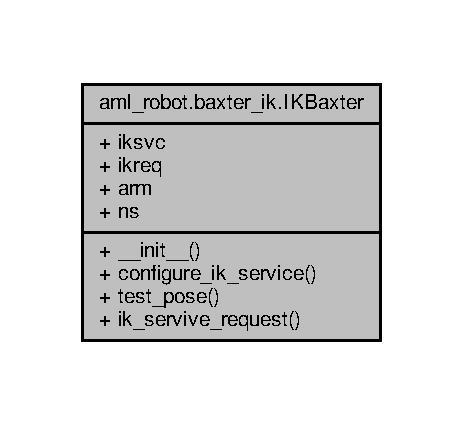
\includegraphics[width=222pt]{classaml__robot_1_1baxter__ik_1_1_i_k_baxter__coll__graph}
\end{center}
\end{figure}
\subsection*{Public Member Functions}
\begin{DoxyCompactItemize}
\item 
\hypertarget{classaml__robot_1_1baxter__ik_1_1_i_k_baxter_acdcbd683c692f89daec2685a9ec2e623}{def {\bfseries \-\_\-\-\_\-init\-\_\-\-\_\-}}\label{classaml__robot_1_1baxter__ik_1_1_i_k_baxter_acdcbd683c692f89daec2685a9ec2e623}

\item 
\hypertarget{classaml__robot_1_1baxter__ik_1_1_i_k_baxter_a6985adef358e80b1924292508a707a66}{def {\bfseries configure\-\_\-ik\-\_\-service}}\label{classaml__robot_1_1baxter__ik_1_1_i_k_baxter_a6985adef358e80b1924292508a707a66}

\item 
\hypertarget{classaml__robot_1_1baxter__ik_1_1_i_k_baxter_a87fb9334e61c8d42b4ff2c5e00402b98}{def {\bfseries test\-\_\-pose}}\label{classaml__robot_1_1baxter__ik_1_1_i_k_baxter_a87fb9334e61c8d42b4ff2c5e00402b98}

\item 
\hypertarget{classaml__robot_1_1baxter__ik_1_1_i_k_baxter_a306f472f1d9fd2105c6d42f092bf476c}{def {\bfseries ik\-\_\-servive\-\_\-request}}\label{classaml__robot_1_1baxter__ik_1_1_i_k_baxter_a306f472f1d9fd2105c6d42f092bf476c}

\end{DoxyCompactItemize}
\subsection*{Public Attributes}
\begin{DoxyCompactItemize}
\item 
\hypertarget{classaml__robot_1_1baxter__ik_1_1_i_k_baxter_a8febd21258f15a3721ecdddd275c9bef}{{\bfseries iksvc}}\label{classaml__robot_1_1baxter__ik_1_1_i_k_baxter_a8febd21258f15a3721ecdddd275c9bef}

\item 
\hypertarget{classaml__robot_1_1baxter__ik_1_1_i_k_baxter_ac3a37bd5bdcafced7d11cff004d5a5da}{{\bfseries ikreq}}\label{classaml__robot_1_1baxter__ik_1_1_i_k_baxter_ac3a37bd5bdcafced7d11cff004d5a5da}

\item 
\hypertarget{classaml__robot_1_1baxter__ik_1_1_i_k_baxter_a31eb6a0623788ecb628c413f6c1cf85a}{{\bfseries arm}}\label{classaml__robot_1_1baxter__ik_1_1_i_k_baxter_a31eb6a0623788ecb628c413f6c1cf85a}

\item 
\hypertarget{classaml__robot_1_1baxter__ik_1_1_i_k_baxter_a006f01e493d58ff9db613d66baa07a63}{{\bfseries ns}}\label{classaml__robot_1_1baxter__ik_1_1_i_k_baxter_a006f01e493d58ff9db613d66baa07a63}

\end{DoxyCompactItemize}


The documentation for this class was generated from the following file\-:\begin{DoxyCompactItemize}
\item 
aml\-\_\-robot/src/aml\-\_\-robot/baxter\-\_\-ik.\-py\end{DoxyCompactItemize}

\hypertarget{classaml__ctrl_1_1controllers_1_1js__controller_1_1_j_s_controller}{\section{aml\-\_\-ctrl.\-controllers.\-js\-\_\-controller.\-J\-S\-Controller Class Reference}
\label{classaml__ctrl_1_1controllers_1_1js__controller_1_1_j_s_controller}\index{aml\-\_\-ctrl.\-controllers.\-js\-\_\-controller.\-J\-S\-Controller@{aml\-\_\-ctrl.\-controllers.\-js\-\_\-controller.\-J\-S\-Controller}}
}


Inheritance diagram for aml\-\_\-ctrl.\-controllers.\-js\-\_\-controller.\-J\-S\-Controller\-:\nopagebreak
\begin{figure}[H]
\begin{center}
\leavevmode
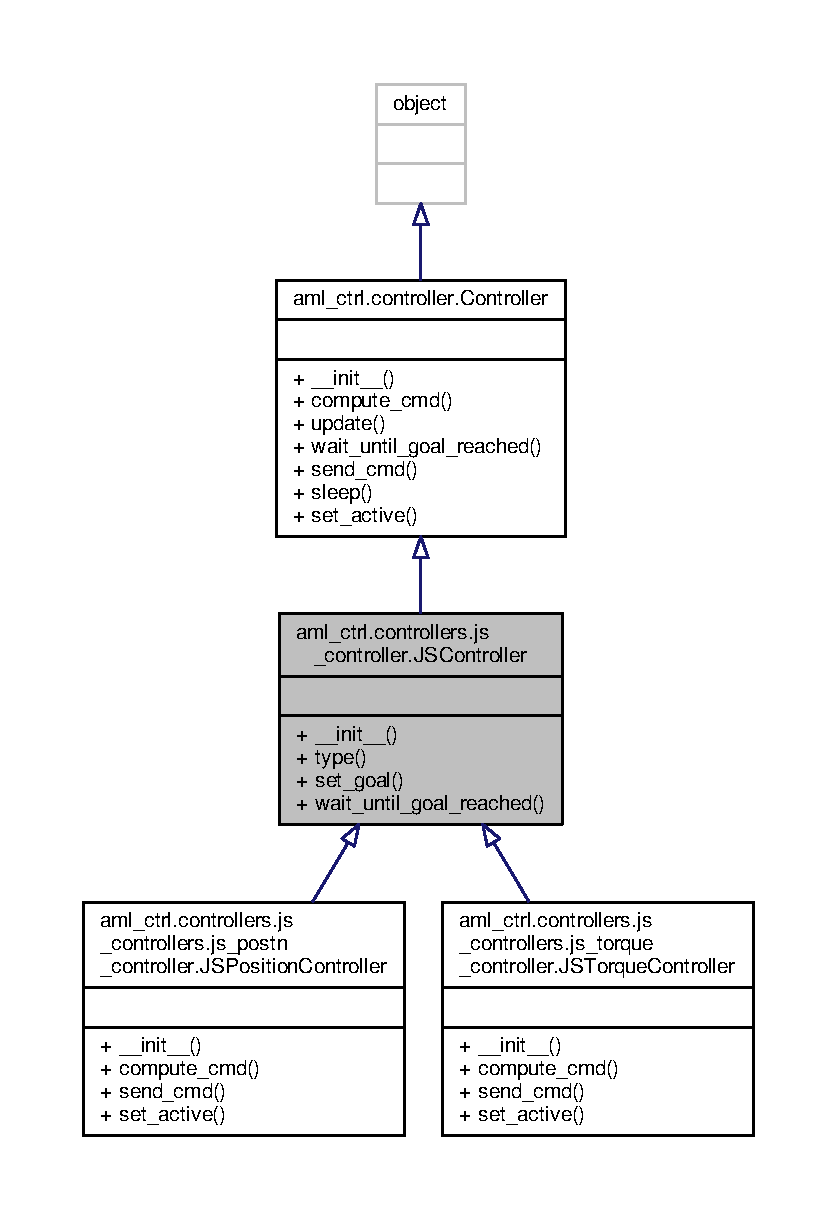
\includegraphics[width=350pt]{classaml__ctrl_1_1controllers_1_1js__controller_1_1_j_s_controller__inherit__graph}
\end{center}
\end{figure}


Collaboration diagram for aml\-\_\-ctrl.\-controllers.\-js\-\_\-controller.\-J\-S\-Controller\-:\nopagebreak
\begin{figure}[H]
\begin{center}
\leavevmode
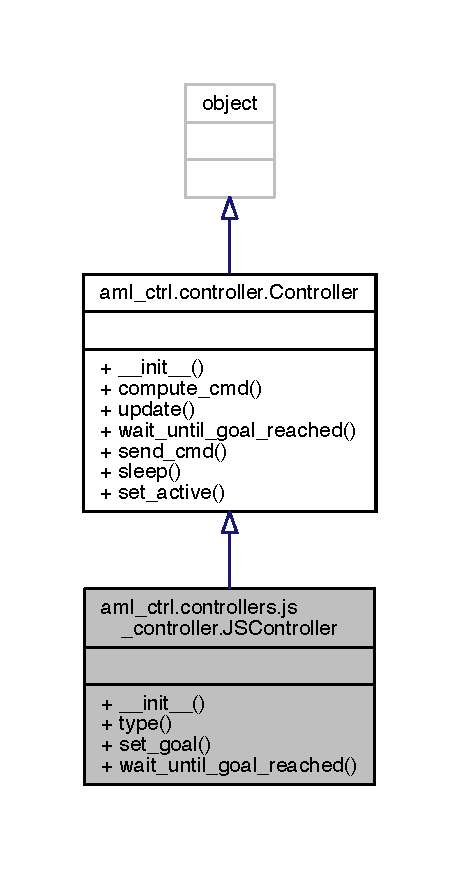
\includegraphics[width=218pt]{classaml__ctrl_1_1controllers_1_1js__controller_1_1_j_s_controller__coll__graph}
\end{center}
\end{figure}
\subsection*{Public Member Functions}
\begin{DoxyCompactItemize}
\item 
\hypertarget{classaml__ctrl_1_1controllers_1_1js__controller_1_1_j_s_controller_a1be5960e312e049110b8991d51210cfe}{def {\bfseries \-\_\-\-\_\-init\-\_\-\-\_\-}}\label{classaml__ctrl_1_1controllers_1_1js__controller_1_1_j_s_controller_a1be5960e312e049110b8991d51210cfe}

\item 
\hypertarget{classaml__ctrl_1_1controllers_1_1js__controller_1_1_j_s_controller_a79e68c4d8dacce86034685b456d73f35}{def {\bfseries type}}\label{classaml__ctrl_1_1controllers_1_1js__controller_1_1_j_s_controller_a79e68c4d8dacce86034685b456d73f35}

\item 
\hypertarget{classaml__ctrl_1_1controllers_1_1js__controller_1_1_j_s_controller_a6fc08eab26adc2e6b8203000c6354995}{def {\bfseries set\-\_\-goal}}\label{classaml__ctrl_1_1controllers_1_1js__controller_1_1_j_s_controller_a6fc08eab26adc2e6b8203000c6354995}

\item 
\hypertarget{classaml__ctrl_1_1controllers_1_1js__controller_1_1_j_s_controller_abe8dc6b50975e05b50c4f7ab2c2caf7c}{def {\bfseries wait\-\_\-until\-\_\-goal\-\_\-reached}}\label{classaml__ctrl_1_1controllers_1_1js__controller_1_1_j_s_controller_abe8dc6b50975e05b50c4f7ab2c2caf7c}

\end{DoxyCompactItemize}


The documentation for this class was generated from the following file\-:\begin{DoxyCompactItemize}
\item 
aml\-\_\-ctrl/src/aml\-\_\-ctrl/controllers/js\-\_\-controller.\-py\end{DoxyCompactItemize}

\hypertarget{classaml__ctrl_1_1controllers_1_1js__controllers_1_1js__postn__controller_1_1_j_s_position_controller}{\section{aml\-\_\-ctrl.\-controllers.\-js\-\_\-controllers.\-js\-\_\-postn\-\_\-controller.\-J\-S\-Position\-Controller Class Reference}
\label{classaml__ctrl_1_1controllers_1_1js__controllers_1_1js__postn__controller_1_1_j_s_position_controller}\index{aml\-\_\-ctrl.\-controllers.\-js\-\_\-controllers.\-js\-\_\-postn\-\_\-controller.\-J\-S\-Position\-Controller@{aml\-\_\-ctrl.\-controllers.\-js\-\_\-controllers.\-js\-\_\-postn\-\_\-controller.\-J\-S\-Position\-Controller}}
}


Inheritance diagram for aml\-\_\-ctrl.\-controllers.\-js\-\_\-controllers.\-js\-\_\-postn\-\_\-controller.\-J\-S\-Position\-Controller\-:
\nopagebreak
\begin{figure}[H]
\begin{center}
\leavevmode
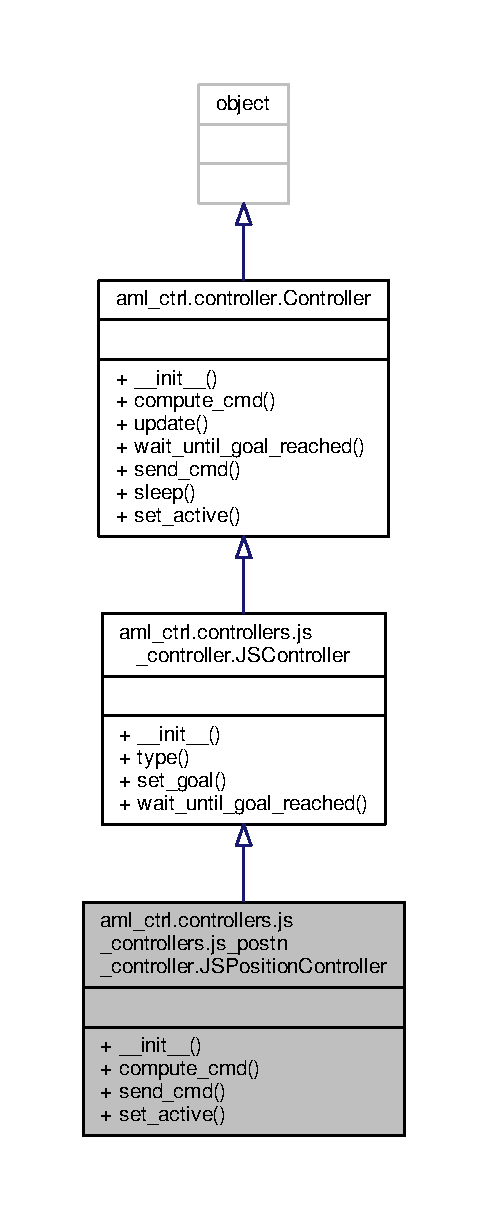
\includegraphics[height=550pt]{classaml__ctrl_1_1controllers_1_1js__controllers_1_1js__postn__controller_1_1_j_s_position_controller__inherit__graph}
\end{center}
\end{figure}


Collaboration diagram for aml\-\_\-ctrl.\-controllers.\-js\-\_\-controllers.\-js\-\_\-postn\-\_\-controller.\-J\-S\-Position\-Controller\-:
\nopagebreak
\begin{figure}[H]
\begin{center}
\leavevmode
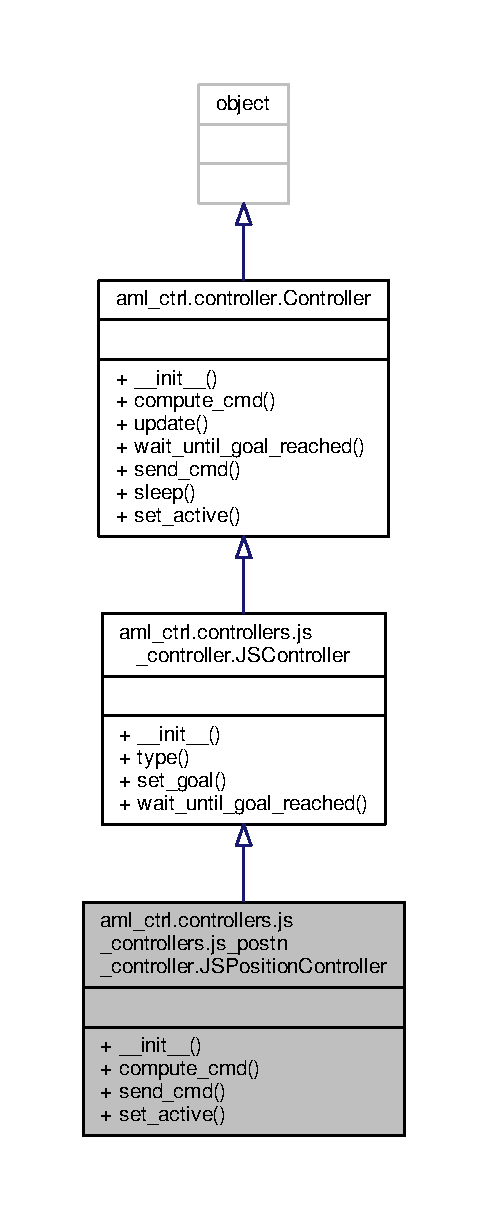
\includegraphics[height=550pt]{classaml__ctrl_1_1controllers_1_1js__controllers_1_1js__postn__controller_1_1_j_s_position_controller__coll__graph}
\end{center}
\end{figure}
\subsection*{Public Member Functions}
\begin{DoxyCompactItemize}
\item 
\hypertarget{classaml__ctrl_1_1controllers_1_1js__controllers_1_1js__postn__controller_1_1_j_s_position_controller_ac463a885a8605d9493b750bb479cb6a8}{def {\bfseries \-\_\-\-\_\-init\-\_\-\-\_\-}}\label{classaml__ctrl_1_1controllers_1_1js__controllers_1_1js__postn__controller_1_1_j_s_position_controller_ac463a885a8605d9493b750bb479cb6a8}

\item 
\hypertarget{classaml__ctrl_1_1controllers_1_1js__controllers_1_1js__postn__controller_1_1_j_s_position_controller_a17033e0eba8bfa1c3a2681089feb7bc4}{def {\bfseries compute\-\_\-cmd}}\label{classaml__ctrl_1_1controllers_1_1js__controllers_1_1js__postn__controller_1_1_j_s_position_controller_a17033e0eba8bfa1c3a2681089feb7bc4}

\item 
\hypertarget{classaml__ctrl_1_1controllers_1_1js__controllers_1_1js__postn__controller_1_1_j_s_position_controller_adff2d8a101823f2830097b24c097d01a}{def {\bfseries send\-\_\-cmd}}\label{classaml__ctrl_1_1controllers_1_1js__controllers_1_1js__postn__controller_1_1_j_s_position_controller_adff2d8a101823f2830097b24c097d01a}

\item 
\hypertarget{classaml__ctrl_1_1controllers_1_1js__controllers_1_1js__postn__controller_1_1_j_s_position_controller_a4748c9f80fbbc3b24326e295d0755482}{def {\bfseries set\-\_\-active}}\label{classaml__ctrl_1_1controllers_1_1js__controllers_1_1js__postn__controller_1_1_j_s_position_controller_a4748c9f80fbbc3b24326e295d0755482}

\end{DoxyCompactItemize}


The documentation for this class was generated from the following file\-:\begin{DoxyCompactItemize}
\item 
aml\-\_\-ctrl/src/aml\-\_\-ctrl/controllers/js\-\_\-controllers/js\-\_\-postn\-\_\-controller.\-py\end{DoxyCompactItemize}

\hypertarget{classaml__ctrl_1_1controllers_1_1js__controllers_1_1js__torque__controller_1_1_j_s_torque_controller}{}\section{aml\+\_\+ctrl.\+controllers.\+js\+\_\+controllers.\+js\+\_\+torque\+\_\+controller.\+J\+S\+Torque\+Controller Class Reference}
\label{classaml__ctrl_1_1controllers_1_1js__controllers_1_1js__torque__controller_1_1_j_s_torque_controller}\index{aml\+\_\+ctrl.\+controllers.\+js\+\_\+controllers.\+js\+\_\+torque\+\_\+controller.\+J\+S\+Torque\+Controller@{aml\+\_\+ctrl.\+controllers.\+js\+\_\+controllers.\+js\+\_\+torque\+\_\+controller.\+J\+S\+Torque\+Controller}}


Inheritance diagram for aml\+\_\+ctrl.\+controllers.\+js\+\_\+controllers.\+js\+\_\+torque\+\_\+controller.\+J\+S\+Torque\+Controller\+:\nopagebreak
\begin{figure}[H]
\begin{center}
\leavevmode
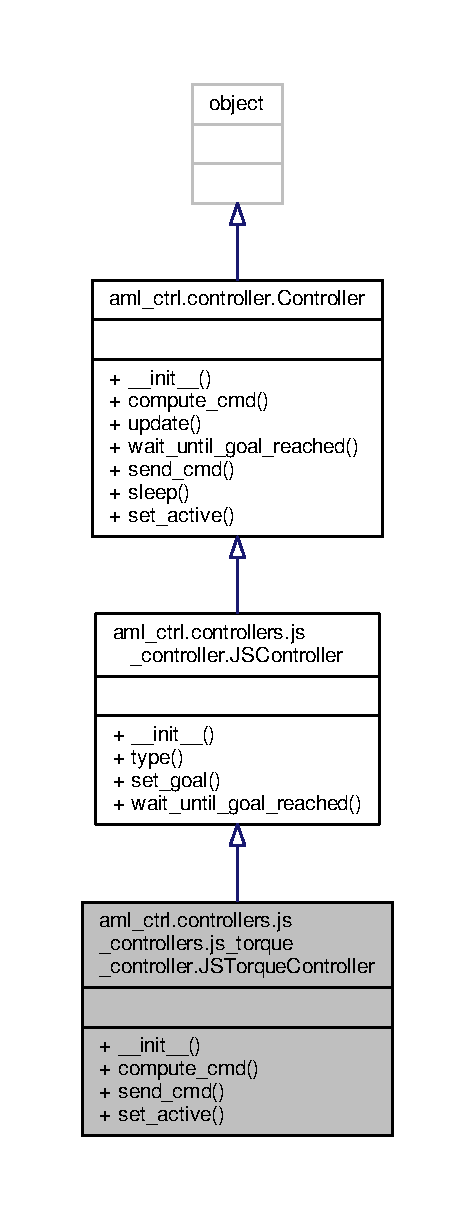
\includegraphics[height=550pt]{classaml__ctrl_1_1controllers_1_1js__controllers_1_1js__torque__controller_1_1_j_s_torque_controller__inherit__graph}
\end{center}
\end{figure}


Collaboration diagram for aml\+\_\+ctrl.\+controllers.\+js\+\_\+controllers.\+js\+\_\+torque\+\_\+controller.\+J\+S\+Torque\+Controller\+:\nopagebreak
\begin{figure}[H]
\begin{center}
\leavevmode
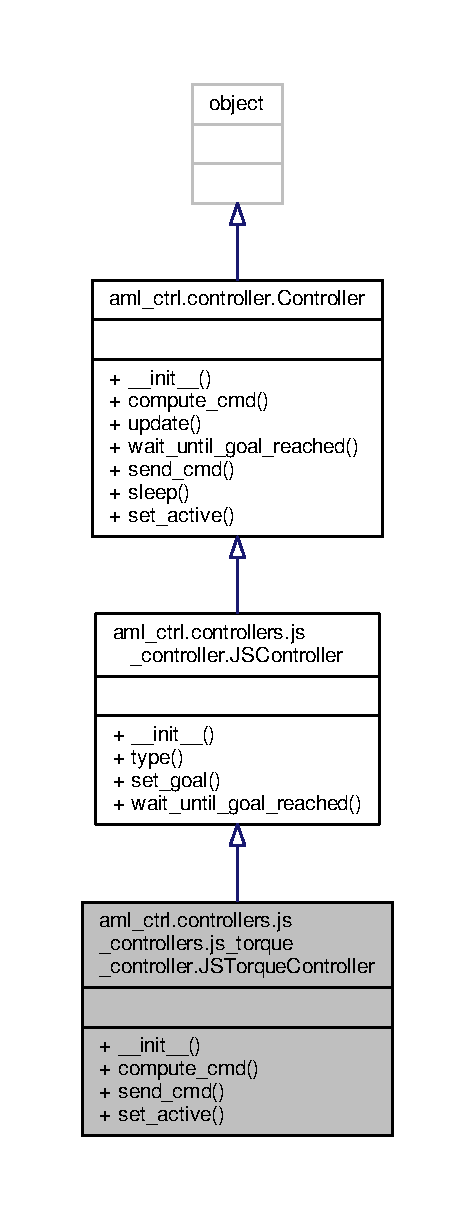
\includegraphics[height=550pt]{classaml__ctrl_1_1controllers_1_1js__controllers_1_1js__torque__controller_1_1_j_s_torque_controller__coll__graph}
\end{center}
\end{figure}
\subsection*{Public Member Functions}
\begin{DoxyCompactItemize}
\item 
\hypertarget{classaml__ctrl_1_1controllers_1_1js__controllers_1_1js__torque__controller_1_1_j_s_torque_controller_a6c4438a0f7de1511e34fff8dd78f6999}{}\label{classaml__ctrl_1_1controllers_1_1js__controllers_1_1js__torque__controller_1_1_j_s_torque_controller_a6c4438a0f7de1511e34fff8dd78f6999} 
def {\bfseries \+\_\+\+\_\+init\+\_\+\+\_\+} (self, robot\+\_\+interface, config=J\+S\+\_\+\+T\+O\+R\+Q\+U\+E\+\_\+\+C\+N\+T\+LR)
\item 
\hypertarget{classaml__ctrl_1_1controllers_1_1js__controllers_1_1js__torque__controller_1_1_j_s_torque_controller_a1f6cfa660a0b6e9f123c544bac73a8b2}{}\label{classaml__ctrl_1_1controllers_1_1js__controllers_1_1js__torque__controller_1_1_j_s_torque_controller_a1f6cfa660a0b6e9f123c544bac73a8b2} 
def {\bfseries compute\+\_\+cmd} (self, time\+\_\+elapsed)
\item 
\hypertarget{classaml__ctrl_1_1controllers_1_1js__controllers_1_1js__torque__controller_1_1_j_s_torque_controller_a339d1c5d2acc1859605f5c87200a88bf}{}\label{classaml__ctrl_1_1controllers_1_1js__controllers_1_1js__torque__controller_1_1_j_s_torque_controller_a339d1c5d2acc1859605f5c87200a88bf} 
def {\bfseries send\+\_\+cmd} (self, time\+\_\+elapsed)
\item 
\hypertarget{classaml__ctrl_1_1controllers_1_1js__controllers_1_1js__torque__controller_1_1_j_s_torque_controller_ad422e4ee2a27feaa48be0d483ab3132d}{}\label{classaml__ctrl_1_1controllers_1_1js__controllers_1_1js__torque__controller_1_1_j_s_torque_controller_ad422e4ee2a27feaa48be0d483ab3132d} 
def {\bfseries set\+\_\+active} (self, is\+\_\+active)
\end{DoxyCompactItemize}


The documentation for this class was generated from the following file\+:\begin{DoxyCompactItemize}
\item 
aml\+\_\+ctrl/src/aml\+\_\+ctrl/controllers/js\+\_\+controllers/js\+\_\+torque\+\_\+controller.\+py\end{DoxyCompactItemize}

\hypertarget{classaml__ctrl_1_1traj__generator_1_1js__traj__generator_1_1_j_s_traj_generator}{}\section{aml\+\_\+ctrl.\+traj\+\_\+generator.\+js\+\_\+traj\+\_\+generator.\+J\+S\+Traj\+Generator Class Reference}
\label{classaml__ctrl_1_1traj__generator_1_1js__traj__generator_1_1_j_s_traj_generator}\index{aml\+\_\+ctrl.\+traj\+\_\+generator.\+js\+\_\+traj\+\_\+generator.\+J\+S\+Traj\+Generator@{aml\+\_\+ctrl.\+traj\+\_\+generator.\+js\+\_\+traj\+\_\+generator.\+J\+S\+Traj\+Generator}}


Inheritance diagram for aml\+\_\+ctrl.\+traj\+\_\+generator.\+js\+\_\+traj\+\_\+generator.\+J\+S\+Traj\+Generator\+:\nopagebreak
\begin{figure}[H]
\begin{center}
\leavevmode
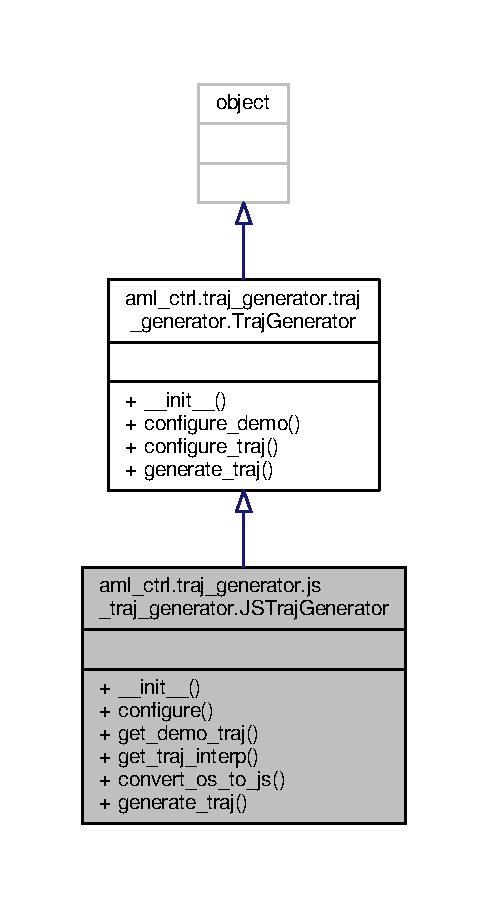
\includegraphics[width=240pt]{classaml__ctrl_1_1traj__generator_1_1js__traj__generator_1_1_j_s_traj_generator__inherit__graph}
\end{center}
\end{figure}


Collaboration diagram for aml\+\_\+ctrl.\+traj\+\_\+generator.\+js\+\_\+traj\+\_\+generator.\+J\+S\+Traj\+Generator\+:\nopagebreak
\begin{figure}[H]
\begin{center}
\leavevmode
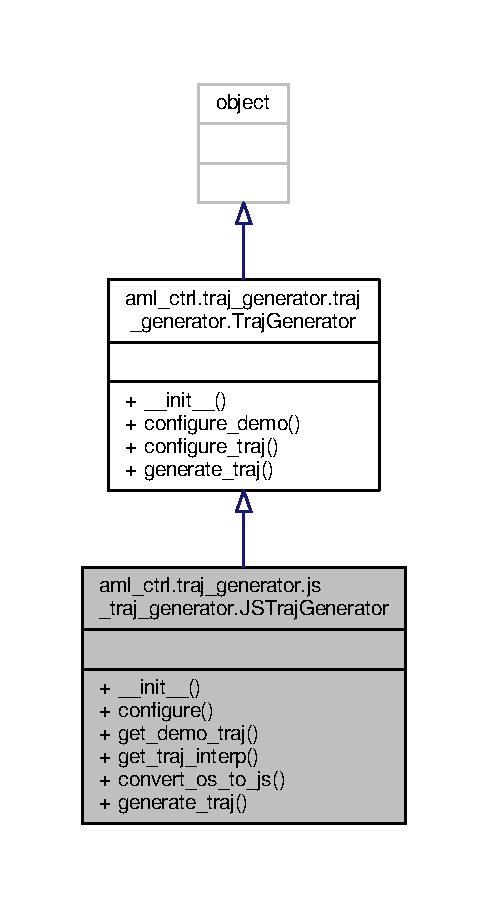
\includegraphics[width=240pt]{classaml__ctrl_1_1traj__generator_1_1js__traj__generator_1_1_j_s_traj_generator__coll__graph}
\end{center}
\end{figure}
\subsection*{Public Member Functions}
\begin{DoxyCompactItemize}
\item 
\hypertarget{classaml__ctrl_1_1traj__generator_1_1js__traj__generator_1_1_j_s_traj_generator_a8f3f80b67d5c1ca0821cd311764636ec}{}\label{classaml__ctrl_1_1traj__generator_1_1js__traj__generator_1_1_j_s_traj_generator_a8f3f80b67d5c1ca0821cd311764636ec} 
def {\bfseries \+\_\+\+\_\+init\+\_\+\+\_\+} (self, load\+\_\+from\+\_\+demo=False, kwargs)
\item 
\hypertarget{classaml__ctrl_1_1traj__generator_1_1js__traj__generator_1_1_j_s_traj_generator_a022b44a0ef727669bb5c5a12b6ed9b44}{}\label{classaml__ctrl_1_1traj__generator_1_1js__traj__generator_1_1_j_s_traj_generator_a022b44a0ef727669bb5c5a12b6ed9b44} 
def {\bfseries configure} (self, robot\+\_\+interface)
\item 
\hypertarget{classaml__ctrl_1_1traj__generator_1_1js__traj__generator_1_1_j_s_traj_generator_ad5f065b319964c3e6640c700eabf2361}{}\label{classaml__ctrl_1_1traj__generator_1_1js__traj__generator_1_1_j_s_traj_generator_ad5f065b319964c3e6640c700eabf2361} 
def {\bfseries get\+\_\+demo\+\_\+traj} (self)
\item 
\hypertarget{classaml__ctrl_1_1traj__generator_1_1js__traj__generator_1_1_j_s_traj_generator_a8844409ef5da594ac029efbb4c60f617}{}\label{classaml__ctrl_1_1traj__generator_1_1js__traj__generator_1_1_j_s_traj_generator_a8844409ef5da594ac029efbb4c60f617} 
def {\bfseries get\+\_\+traj\+\_\+interp} (self)
\item 
\hypertarget{classaml__ctrl_1_1traj__generator_1_1js__traj__generator_1_1_j_s_traj_generator_a8aeb635dc050800d6dad4a7f34d32f26}{}\label{classaml__ctrl_1_1traj__generator_1_1js__traj__generator_1_1_j_s_traj_generator_a8aeb635dc050800d6dad4a7f34d32f26} 
def {\bfseries convert\+\_\+os\+\_\+to\+\_\+js} (self, os\+\_\+traj=None)
\item 
\hypertarget{classaml__ctrl_1_1traj__generator_1_1js__traj__generator_1_1_j_s_traj_generator_a449ff9de50f0939e27a5ae11e9c4cfb0}{}\label{classaml__ctrl_1_1traj__generator_1_1js__traj__generator_1_1_j_s_traj_generator_a449ff9de50f0939e27a5ae11e9c4cfb0} 
def {\bfseries generate\+\_\+traj} (self)
\end{DoxyCompactItemize}


The documentation for this class was generated from the following file\+:\begin{DoxyCompactItemize}
\item 
aml\+\_\+ctrl/src/aml\+\_\+ctrl/traj\+\_\+generator/js\+\_\+traj\+\_\+generator.\+py\end{DoxyCompactItemize}

\hypertarget{classaml__lfd_1_1lfd_1_1_lf_d}{\section{aml\-\_\-lfd.\-lfd.\-Lf\-D Class Reference}
\label{classaml__lfd_1_1lfd_1_1_lf_d}\index{aml\-\_\-lfd.\-lfd.\-Lf\-D@{aml\-\_\-lfd.\-lfd.\-Lf\-D}}
}


Inheritance diagram for aml\-\_\-lfd.\-lfd.\-Lf\-D\-:\nopagebreak
\begin{figure}[H]
\begin{center}
\leavevmode
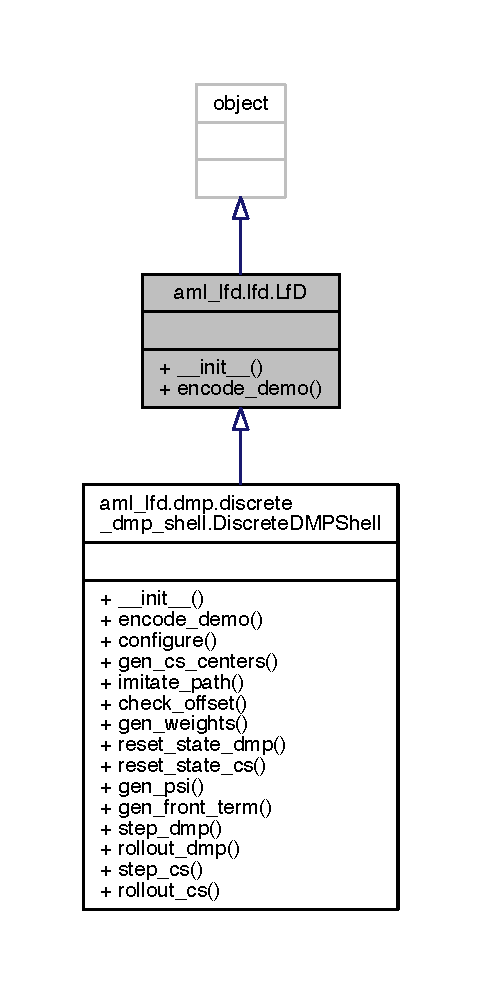
\includegraphics[width=172pt]{classaml__lfd_1_1lfd_1_1_lf_d__inherit__graph}
\end{center}
\end{figure}


Collaboration diagram for aml\-\_\-lfd.\-lfd.\-Lf\-D\-:\nopagebreak
\begin{figure}[H]
\begin{center}
\leavevmode
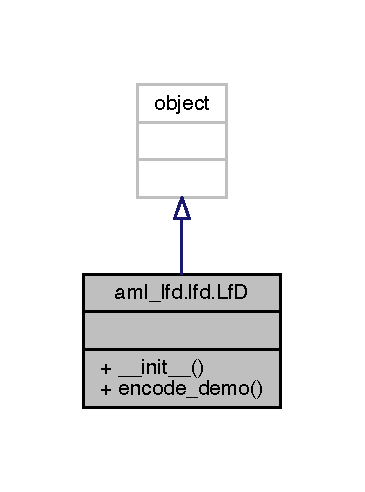
\includegraphics[width=172pt]{classaml__lfd_1_1lfd_1_1_lf_d__coll__graph}
\end{center}
\end{figure}
\subsection*{Public Member Functions}
\begin{DoxyCompactItemize}
\item 
\hypertarget{classaml__lfd_1_1lfd_1_1_lf_d_aab9046d6d3824e7bfeea0eddbfe5054f}{def {\bfseries \-\_\-\-\_\-init\-\_\-\-\_\-}}\label{classaml__lfd_1_1lfd_1_1_lf_d_aab9046d6d3824e7bfeea0eddbfe5054f}

\item 
\hypertarget{classaml__lfd_1_1lfd_1_1_lf_d_a0f3dff0ab9b2d70047d3a2679cd5152e}{def {\bfseries encode\-\_\-demo}}\label{classaml__lfd_1_1lfd_1_1_lf_d_a0f3dff0ab9b2d70047d3a2679cd5152e}

\end{DoxyCompactItemize}


The documentation for this class was generated from the following file\-:\begin{DoxyCompactItemize}
\item 
aml\-\_\-lfd/src/aml\-\_\-lfd/lfd.\-py\end{DoxyCompactItemize}

\hypertarget{classaml__ctrl_1_1utilities_1_1lin__interp_1_1_lin_interp}{\section{aml\-\_\-ctrl.\-utilities.\-lin\-\_\-interp.\-Lin\-Interp Class Reference}
\label{classaml__ctrl_1_1utilities_1_1lin__interp_1_1_lin_interp}\index{aml\-\_\-ctrl.\-utilities.\-lin\-\_\-interp.\-Lin\-Interp@{aml\-\_\-ctrl.\-utilities.\-lin\-\_\-interp.\-Lin\-Interp}}
}


Collaboration diagram for aml\-\_\-ctrl.\-utilities.\-lin\-\_\-interp.\-Lin\-Interp\-:
\nopagebreak
\begin{figure}[H]
\begin{center}
\leavevmode
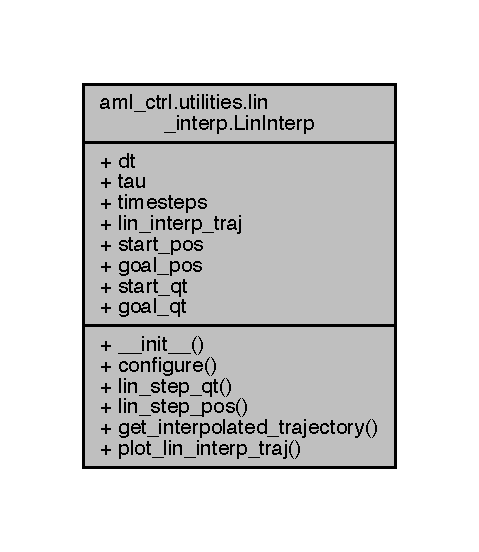
\includegraphics[width=226pt]{classaml__ctrl_1_1utilities_1_1lin__interp_1_1_lin_interp__coll__graph}
\end{center}
\end{figure}
\subsection*{Public Member Functions}
\begin{DoxyCompactItemize}
\item 
\hypertarget{classaml__ctrl_1_1utilities_1_1lin__interp_1_1_lin_interp_a1e35790a94c93ae7d3d8024028c550ff}{def {\bfseries \-\_\-\-\_\-init\-\_\-\-\_\-}}\label{classaml__ctrl_1_1utilities_1_1lin__interp_1_1_lin_interp_a1e35790a94c93ae7d3d8024028c550ff}

\item 
\hypertarget{classaml__ctrl_1_1utilities_1_1lin__interp_1_1_lin_interp_a14a7de9dcf847e85448a5e5b1d061e94}{def {\bfseries configure}}\label{classaml__ctrl_1_1utilities_1_1lin__interp_1_1_lin_interp_a14a7de9dcf847e85448a5e5b1d061e94}

\item 
\hypertarget{classaml__ctrl_1_1utilities_1_1lin__interp_1_1_lin_interp_a4ed2ce1b4e7cc2b115247fb09a7847ad}{def {\bfseries lin\-\_\-step\-\_\-qt}}\label{classaml__ctrl_1_1utilities_1_1lin__interp_1_1_lin_interp_a4ed2ce1b4e7cc2b115247fb09a7847ad}

\item 
\hypertarget{classaml__ctrl_1_1utilities_1_1lin__interp_1_1_lin_interp_a4938f92638c8384e71cbdc9ca57fd0e0}{def {\bfseries lin\-\_\-step\-\_\-pos}}\label{classaml__ctrl_1_1utilities_1_1lin__interp_1_1_lin_interp_a4938f92638c8384e71cbdc9ca57fd0e0}

\item 
\hypertarget{classaml__ctrl_1_1utilities_1_1lin__interp_1_1_lin_interp_a50602f7c9cfa8746de0fda436e6b6283}{def {\bfseries get\-\_\-interpolated\-\_\-trajectory}}\label{classaml__ctrl_1_1utilities_1_1lin__interp_1_1_lin_interp_a50602f7c9cfa8746de0fda436e6b6283}

\item 
\hypertarget{classaml__ctrl_1_1utilities_1_1lin__interp_1_1_lin_interp_ab08c5f7742c601b1523f7d82216e2f3e}{def {\bfseries plot\-\_\-lin\-\_\-interp\-\_\-traj}}\label{classaml__ctrl_1_1utilities_1_1lin__interp_1_1_lin_interp_ab08c5f7742c601b1523f7d82216e2f3e}

\end{DoxyCompactItemize}
\subsection*{Public Attributes}
\begin{DoxyCompactItemize}
\item 
\hypertarget{classaml__ctrl_1_1utilities_1_1lin__interp_1_1_lin_interp_a91ce8d62c538477b2e4e30cc604b9d60}{{\bfseries dt}}\label{classaml__ctrl_1_1utilities_1_1lin__interp_1_1_lin_interp_a91ce8d62c538477b2e4e30cc604b9d60}

\item 
\hypertarget{classaml__ctrl_1_1utilities_1_1lin__interp_1_1_lin_interp_a3a9296ff1896b9de1f43ebf138554658}{{\bfseries tau}}\label{classaml__ctrl_1_1utilities_1_1lin__interp_1_1_lin_interp_a3a9296ff1896b9de1f43ebf138554658}

\item 
\hypertarget{classaml__ctrl_1_1utilities_1_1lin__interp_1_1_lin_interp_a601fd091f2e367969d20dced930e84ca}{{\bfseries timesteps}}\label{classaml__ctrl_1_1utilities_1_1lin__interp_1_1_lin_interp_a601fd091f2e367969d20dced930e84ca}

\item 
\hypertarget{classaml__ctrl_1_1utilities_1_1lin__interp_1_1_lin_interp_a636787254c4170344140b25b54139782}{{\bfseries lin\-\_\-interp\-\_\-traj}}\label{classaml__ctrl_1_1utilities_1_1lin__interp_1_1_lin_interp_a636787254c4170344140b25b54139782}

\item 
\hypertarget{classaml__ctrl_1_1utilities_1_1lin__interp_1_1_lin_interp_af6583e2f56c7732af967927541ed01ce}{{\bfseries start\-\_\-pos}}\label{classaml__ctrl_1_1utilities_1_1lin__interp_1_1_lin_interp_af6583e2f56c7732af967927541ed01ce}

\item 
\hypertarget{classaml__ctrl_1_1utilities_1_1lin__interp_1_1_lin_interp_a2827d5e7e445519eb94643982b8fbe15}{{\bfseries goal\-\_\-pos}}\label{classaml__ctrl_1_1utilities_1_1lin__interp_1_1_lin_interp_a2827d5e7e445519eb94643982b8fbe15}

\item 
\hypertarget{classaml__ctrl_1_1utilities_1_1lin__interp_1_1_lin_interp_a8e59d6ea4a99b6ef7ed6a8acaac632d4}{{\bfseries start\-\_\-qt}}\label{classaml__ctrl_1_1utilities_1_1lin__interp_1_1_lin_interp_a8e59d6ea4a99b6ef7ed6a8acaac632d4}

\item 
\hypertarget{classaml__ctrl_1_1utilities_1_1lin__interp_1_1_lin_interp_ac042c31929df9c729e392ee7bc72a84a}{{\bfseries goal\-\_\-qt}}\label{classaml__ctrl_1_1utilities_1_1lin__interp_1_1_lin_interp_ac042c31929df9c729e392ee7bc72a84a}

\end{DoxyCompactItemize}


The documentation for this class was generated from the following file\-:\begin{DoxyCompactItemize}
\item 
aml\-\_\-ctrl/src/aml\-\_\-ctrl/utilities/lin\-\_\-interp.\-py\end{DoxyCompactItemize}

\hypertarget{classaml__lfd_1_1lqr_1_1lqr__traj__follow_1_1_l_q_r_traj_follow}{\section{aml\-\_\-lfd.\-lqr.\-lqr\-\_\-traj\-\_\-follow.\-L\-Q\-R\-Traj\-Follow Class Reference}
\label{classaml__lfd_1_1lqr_1_1lqr__traj__follow_1_1_l_q_r_traj_follow}\index{aml\-\_\-lfd.\-lqr.\-lqr\-\_\-traj\-\_\-follow.\-L\-Q\-R\-Traj\-Follow@{aml\-\_\-lfd.\-lqr.\-lqr\-\_\-traj\-\_\-follow.\-L\-Q\-R\-Traj\-Follow}}
}


Collaboration diagram for aml\-\_\-lfd.\-lqr.\-lqr\-\_\-traj\-\_\-follow.\-L\-Q\-R\-Traj\-Follow\-:
\nopagebreak
\begin{figure}[H]
\begin{center}
\leavevmode
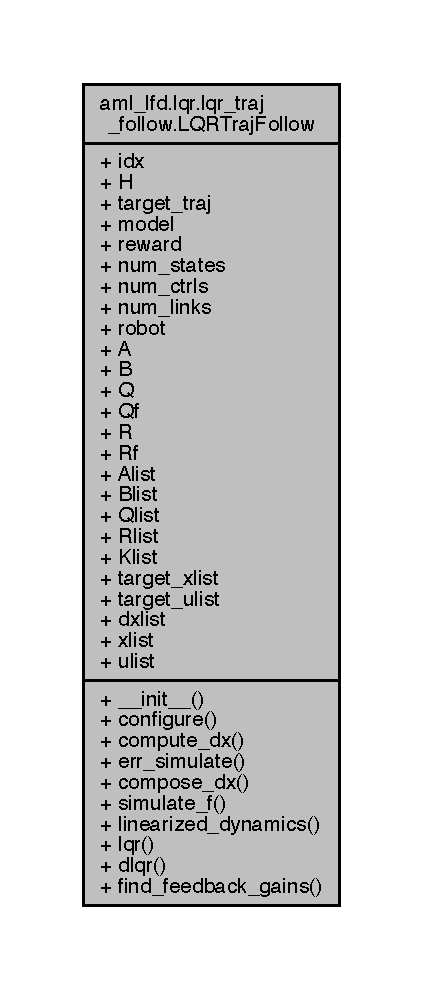
\includegraphics[width=200pt]{classaml__lfd_1_1lqr_1_1lqr__traj__follow_1_1_l_q_r_traj_follow__coll__graph}
\end{center}
\end{figure}
\subsection*{Public Member Functions}
\begin{DoxyCompactItemize}
\item 
\hypertarget{classaml__lfd_1_1lqr_1_1lqr__traj__follow_1_1_l_q_r_traj_follow_acbb05476cbb16e8e238eaecc375bd062}{def {\bfseries \-\_\-\-\_\-init\-\_\-\-\_\-}}\label{classaml__lfd_1_1lqr_1_1lqr__traj__follow_1_1_l_q_r_traj_follow_acbb05476cbb16e8e238eaecc375bd062}

\item 
\hypertarget{classaml__lfd_1_1lqr_1_1lqr__traj__follow_1_1_l_q_r_traj_follow_ac4e443bc2b3b58dfb909dd1084a11a11}{def {\bfseries configure}}\label{classaml__lfd_1_1lqr_1_1lqr__traj__follow_1_1_l_q_r_traj_follow_ac4e443bc2b3b58dfb909dd1084a11a11}

\item 
\hypertarget{classaml__lfd_1_1lqr_1_1lqr__traj__follow_1_1_l_q_r_traj_follow_a36a88a75e595f13d0b6717f35fa5ab91}{def {\bfseries compute\-\_\-dx}}\label{classaml__lfd_1_1lqr_1_1lqr__traj__follow_1_1_l_q_r_traj_follow_a36a88a75e595f13d0b6717f35fa5ab91}

\item 
\hypertarget{classaml__lfd_1_1lqr_1_1lqr__traj__follow_1_1_l_q_r_traj_follow_a7fd528502e2e6f355dd0a78e85edbde0}{def {\bfseries err\-\_\-simulate}}\label{classaml__lfd_1_1lqr_1_1lqr__traj__follow_1_1_l_q_r_traj_follow_a7fd528502e2e6f355dd0a78e85edbde0}

\item 
\hypertarget{classaml__lfd_1_1lqr_1_1lqr__traj__follow_1_1_l_q_r_traj_follow_a92582e75cb2c7fb600ccf28d0eead6e9}{def {\bfseries compose\-\_\-dx}}\label{classaml__lfd_1_1lqr_1_1lqr__traj__follow_1_1_l_q_r_traj_follow_a92582e75cb2c7fb600ccf28d0eead6e9}

\item 
\hypertarget{classaml__lfd_1_1lqr_1_1lqr__traj__follow_1_1_l_q_r_traj_follow_ae44942a2b3f38265f5864e112e713a4e}{def {\bfseries simulate\-\_\-f}}\label{classaml__lfd_1_1lqr_1_1lqr__traj__follow_1_1_l_q_r_traj_follow_ae44942a2b3f38265f5864e112e713a4e}

\item 
\hypertarget{classaml__lfd_1_1lqr_1_1lqr__traj__follow_1_1_l_q_r_traj_follow_a2b582169fbc023aeb0121fea485cc0ff}{def {\bfseries linearized\-\_\-dynamics}}\label{classaml__lfd_1_1lqr_1_1lqr__traj__follow_1_1_l_q_r_traj_follow_a2b582169fbc023aeb0121fea485cc0ff}

\item 
\hypertarget{classaml__lfd_1_1lqr_1_1lqr__traj__follow_1_1_l_q_r_traj_follow_a690d75d9e9512c773502199444480685}{def {\bfseries lqr}}\label{classaml__lfd_1_1lqr_1_1lqr__traj__follow_1_1_l_q_r_traj_follow_a690d75d9e9512c773502199444480685}

\item 
\hypertarget{classaml__lfd_1_1lqr_1_1lqr__traj__follow_1_1_l_q_r_traj_follow_aa05b359efc9d1779ae81ca0dd3525467}{def {\bfseries dlqr}}\label{classaml__lfd_1_1lqr_1_1lqr__traj__follow_1_1_l_q_r_traj_follow_aa05b359efc9d1779ae81ca0dd3525467}

\item 
\hypertarget{classaml__lfd_1_1lqr_1_1lqr__traj__follow_1_1_l_q_r_traj_follow_adec42df243dc0661ce780b509a714876}{def {\bfseries find\-\_\-feedback\-\_\-gains}}\label{classaml__lfd_1_1lqr_1_1lqr__traj__follow_1_1_l_q_r_traj_follow_adec42df243dc0661ce780b509a714876}

\end{DoxyCompactItemize}
\subsection*{Public Attributes}
\begin{DoxyCompactItemize}
\item 
\hypertarget{classaml__lfd_1_1lqr_1_1lqr__traj__follow_1_1_l_q_r_traj_follow_acdfe028943c87b025cf7fbc06ef70fd0}{{\bfseries idx}}\label{classaml__lfd_1_1lqr_1_1lqr__traj__follow_1_1_l_q_r_traj_follow_acdfe028943c87b025cf7fbc06ef70fd0}

\item 
\hypertarget{classaml__lfd_1_1lqr_1_1lqr__traj__follow_1_1_l_q_r_traj_follow_ab761a4111b05cec415c4a3216084f77d}{{\bfseries H}}\label{classaml__lfd_1_1lqr_1_1lqr__traj__follow_1_1_l_q_r_traj_follow_ab761a4111b05cec415c4a3216084f77d}

\item 
\hypertarget{classaml__lfd_1_1lqr_1_1lqr__traj__follow_1_1_l_q_r_traj_follow_a8f217f0b7f45e88af0249baffe6b9e24}{{\bfseries target\-\_\-traj}}\label{classaml__lfd_1_1lqr_1_1lqr__traj__follow_1_1_l_q_r_traj_follow_a8f217f0b7f45e88af0249baffe6b9e24}

\item 
\hypertarget{classaml__lfd_1_1lqr_1_1lqr__traj__follow_1_1_l_q_r_traj_follow_a5a99d1280c2ca955b078734bc923453d}{{\bfseries model}}\label{classaml__lfd_1_1lqr_1_1lqr__traj__follow_1_1_l_q_r_traj_follow_a5a99d1280c2ca955b078734bc923453d}

\item 
\hypertarget{classaml__lfd_1_1lqr_1_1lqr__traj__follow_1_1_l_q_r_traj_follow_ae74ea09c332230dd2d3a7ea018d2b4f0}{{\bfseries reward}}\label{classaml__lfd_1_1lqr_1_1lqr__traj__follow_1_1_l_q_r_traj_follow_ae74ea09c332230dd2d3a7ea018d2b4f0}

\item 
\hypertarget{classaml__lfd_1_1lqr_1_1lqr__traj__follow_1_1_l_q_r_traj_follow_a90c1612252d53e6cc2c748efd08cc144}{{\bfseries num\-\_\-states}}\label{classaml__lfd_1_1lqr_1_1lqr__traj__follow_1_1_l_q_r_traj_follow_a90c1612252d53e6cc2c748efd08cc144}

\item 
\hypertarget{classaml__lfd_1_1lqr_1_1lqr__traj__follow_1_1_l_q_r_traj_follow_a7636aa71830621dfc55a820451f06c69}{{\bfseries num\-\_\-ctrls}}\label{classaml__lfd_1_1lqr_1_1lqr__traj__follow_1_1_l_q_r_traj_follow_a7636aa71830621dfc55a820451f06c69}

\item 
\hypertarget{classaml__lfd_1_1lqr_1_1lqr__traj__follow_1_1_l_q_r_traj_follow_a7de94731c6015deb36958adbc45b50b3}{{\bfseries num\-\_\-links}}\label{classaml__lfd_1_1lqr_1_1lqr__traj__follow_1_1_l_q_r_traj_follow_a7de94731c6015deb36958adbc45b50b3}

\item 
\hypertarget{classaml__lfd_1_1lqr_1_1lqr__traj__follow_1_1_l_q_r_traj_follow_a5a5623456a1a207a4b61e40ef3f9bac7}{{\bfseries robot}}\label{classaml__lfd_1_1lqr_1_1lqr__traj__follow_1_1_l_q_r_traj_follow_a5a5623456a1a207a4b61e40ef3f9bac7}

\item 
\hypertarget{classaml__lfd_1_1lqr_1_1lqr__traj__follow_1_1_l_q_r_traj_follow_a7ded951bc3a6aa453117ef453cf81d89}{{\bfseries A}}\label{classaml__lfd_1_1lqr_1_1lqr__traj__follow_1_1_l_q_r_traj_follow_a7ded951bc3a6aa453117ef453cf81d89}

\item 
\hypertarget{classaml__lfd_1_1lqr_1_1lqr__traj__follow_1_1_l_q_r_traj_follow_acdc87fa664772ed3a9249d6409b0ffe9}{{\bfseries B}}\label{classaml__lfd_1_1lqr_1_1lqr__traj__follow_1_1_l_q_r_traj_follow_acdc87fa664772ed3a9249d6409b0ffe9}

\item 
\hypertarget{classaml__lfd_1_1lqr_1_1lqr__traj__follow_1_1_l_q_r_traj_follow_a39a7fada44bbd9d99d11833570dd68a4}{{\bfseries Q}}\label{classaml__lfd_1_1lqr_1_1lqr__traj__follow_1_1_l_q_r_traj_follow_a39a7fada44bbd9d99d11833570dd68a4}

\item 
\hypertarget{classaml__lfd_1_1lqr_1_1lqr__traj__follow_1_1_l_q_r_traj_follow_ab0c18118be7bbbef6a6d016418cdbab1}{{\bfseries Qf}}\label{classaml__lfd_1_1lqr_1_1lqr__traj__follow_1_1_l_q_r_traj_follow_ab0c18118be7bbbef6a6d016418cdbab1}

\item 
\hypertarget{classaml__lfd_1_1lqr_1_1lqr__traj__follow_1_1_l_q_r_traj_follow_a7191995bec2a33ced77e96614dcdfef3}{{\bfseries R}}\label{classaml__lfd_1_1lqr_1_1lqr__traj__follow_1_1_l_q_r_traj_follow_a7191995bec2a33ced77e96614dcdfef3}

\item 
\hypertarget{classaml__lfd_1_1lqr_1_1lqr__traj__follow_1_1_l_q_r_traj_follow_a2f8f716d9c1d04fbf3696b41608431d8}{{\bfseries Rf}}\label{classaml__lfd_1_1lqr_1_1lqr__traj__follow_1_1_l_q_r_traj_follow_a2f8f716d9c1d04fbf3696b41608431d8}

\item 
\hypertarget{classaml__lfd_1_1lqr_1_1lqr__traj__follow_1_1_l_q_r_traj_follow_ada7ee9aef1116f1ba812b16a5d007e2c}{{\bfseries Alist}}\label{classaml__lfd_1_1lqr_1_1lqr__traj__follow_1_1_l_q_r_traj_follow_ada7ee9aef1116f1ba812b16a5d007e2c}

\item 
\hypertarget{classaml__lfd_1_1lqr_1_1lqr__traj__follow_1_1_l_q_r_traj_follow_ad99234f85e754237f6b9981fca8ec1db}{{\bfseries Blist}}\label{classaml__lfd_1_1lqr_1_1lqr__traj__follow_1_1_l_q_r_traj_follow_ad99234f85e754237f6b9981fca8ec1db}

\item 
\hypertarget{classaml__lfd_1_1lqr_1_1lqr__traj__follow_1_1_l_q_r_traj_follow_a3f5c63feb46c1c5f53a7654930405866}{{\bfseries Qlist}}\label{classaml__lfd_1_1lqr_1_1lqr__traj__follow_1_1_l_q_r_traj_follow_a3f5c63feb46c1c5f53a7654930405866}

\item 
\hypertarget{classaml__lfd_1_1lqr_1_1lqr__traj__follow_1_1_l_q_r_traj_follow_a677cefc87aae3e07521793209eb6a23d}{{\bfseries Rlist}}\label{classaml__lfd_1_1lqr_1_1lqr__traj__follow_1_1_l_q_r_traj_follow_a677cefc87aae3e07521793209eb6a23d}

\item 
\hypertarget{classaml__lfd_1_1lqr_1_1lqr__traj__follow_1_1_l_q_r_traj_follow_a5f2bda5589414211230b627c8e3a898c}{{\bfseries Klist}}\label{classaml__lfd_1_1lqr_1_1lqr__traj__follow_1_1_l_q_r_traj_follow_a5f2bda5589414211230b627c8e3a898c}

\item 
\hypertarget{classaml__lfd_1_1lqr_1_1lqr__traj__follow_1_1_l_q_r_traj_follow_aab5b823ec9dc177f15a50fc07fdf76bd}{{\bfseries target\-\_\-xlist}}\label{classaml__lfd_1_1lqr_1_1lqr__traj__follow_1_1_l_q_r_traj_follow_aab5b823ec9dc177f15a50fc07fdf76bd}

\item 
\hypertarget{classaml__lfd_1_1lqr_1_1lqr__traj__follow_1_1_l_q_r_traj_follow_a6543397245f6804c23f2f3adde765f5f}{{\bfseries target\-\_\-ulist}}\label{classaml__lfd_1_1lqr_1_1lqr__traj__follow_1_1_l_q_r_traj_follow_a6543397245f6804c23f2f3adde765f5f}

\item 
\hypertarget{classaml__lfd_1_1lqr_1_1lqr__traj__follow_1_1_l_q_r_traj_follow_a1c7fc079361b526c5af7447d2c744867}{{\bfseries dxlist}}\label{classaml__lfd_1_1lqr_1_1lqr__traj__follow_1_1_l_q_r_traj_follow_a1c7fc079361b526c5af7447d2c744867}

\item 
\hypertarget{classaml__lfd_1_1lqr_1_1lqr__traj__follow_1_1_l_q_r_traj_follow_a35e6ec1df9ee8d476105209def393a1b}{{\bfseries xlist}}\label{classaml__lfd_1_1lqr_1_1lqr__traj__follow_1_1_l_q_r_traj_follow_a35e6ec1df9ee8d476105209def393a1b}

\item 
\hypertarget{classaml__lfd_1_1lqr_1_1lqr__traj__follow_1_1_l_q_r_traj_follow_a9998974c298bc9a488ce3a01d5269544}{{\bfseries ulist}}\label{classaml__lfd_1_1lqr_1_1lqr__traj__follow_1_1_l_q_r_traj_follow_a9998974c298bc9a488ce3a01d5269544}

\end{DoxyCompactItemize}


The documentation for this class was generated from the following file\-:\begin{DoxyCompactItemize}
\item 
aml\-\_\-lfd/src/aml\-\_\-lfd/lqr/lqr\-\_\-traj\-\_\-follow.\-py\end{DoxyCompactItemize}

\hypertarget{class_marker_odometry}{}\section{Marker\+Odometry Class Reference}
\label{class_marker_odometry}\index{Marker\+Odometry@{Marker\+Odometry}}


Collaboration diagram for Marker\+Odometry\+:\nopagebreak
\begin{figure}[H]
\begin{center}
\leavevmode
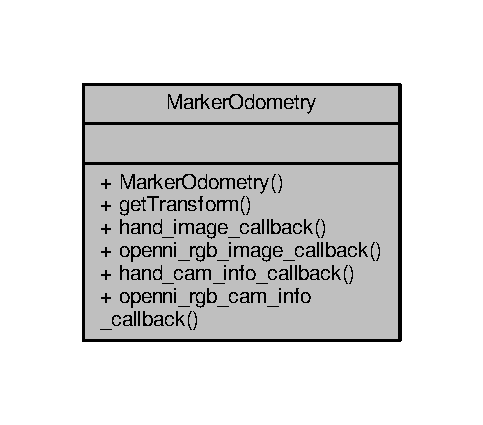
\includegraphics[width=236pt]{class_marker_odometry__coll__graph}
\end{center}
\end{figure}
\subsection*{Public Member Functions}
\begin{DoxyCompactItemize}
\item 
\hypertarget{class_marker_odometry_a991ccdf619ec3c08249f0e8c7b1dfb16}{}\label{class_marker_odometry_a991ccdf619ec3c08249f0e8c7b1dfb16} 
bool {\bfseries get\+Transform} (const std\+::string \&ref\+Frame, const std\+::string \&child\+Frame, tf\+::\+Stamped\+Transform \&transform)
\item 
\hypertarget{class_marker_odometry_a09b1b3528307aa9d2fb98b7e8c923009}{}\label{class_marker_odometry_a09b1b3528307aa9d2fb98b7e8c923009} 
void {\bfseries hand\+\_\+image\+\_\+callback} (const sensor\+\_\+msgs\+::\+Image\+Const\+Ptr \&msg)
\item 
\hypertarget{class_marker_odometry_af6619fc8e9f0183bac7dc40c3a07d097}{}\label{class_marker_odometry_af6619fc8e9f0183bac7dc40c3a07d097} 
void {\bfseries openni\+\_\+rgb\+\_\+image\+\_\+callback} (const sensor\+\_\+msgs\+::\+Image\+Const\+Ptr \&msg)
\item 
\hypertarget{class_marker_odometry_adc0d7677298bed19a3b6a56667c36aeb}{}\label{class_marker_odometry_adc0d7677298bed19a3b6a56667c36aeb} 
void {\bfseries hand\+\_\+cam\+\_\+info\+\_\+callback} (const sensor\+\_\+msgs\+::\+Camera\+Info \&msg)
\item 
\hypertarget{class_marker_odometry_a90f3cc35183a070f578f7f1f57b6c0d8}{}\label{class_marker_odometry_a90f3cc35183a070f578f7f1f57b6c0d8} 
void {\bfseries openni\+\_\+rgb\+\_\+cam\+\_\+info\+\_\+callback} (const sensor\+\_\+msgs\+::\+Camera\+Info \&msg)
\end{DoxyCompactItemize}


The documentation for this class was generated from the following file\+:\begin{DoxyCompactItemize}
\item 
aml\+\_\+calib/src/Marker\+Odometry\+Node.\+cpp\end{DoxyCompactItemize}

\hypertarget{classsrc_1_1aml__dl_1_1mdn_1_1model_1_1mdn__push__inv__model_1_1_m_d_n_push_inverse_model}{}\section{src.\+aml\+\_\+dl.\+mdn.\+model.\+mdn\+\_\+push\+\_\+inv\+\_\+model.\+M\+D\+N\+Push\+Inverse\+Model Class Reference}
\label{classsrc_1_1aml__dl_1_1mdn_1_1model_1_1mdn__push__inv__model_1_1_m_d_n_push_inverse_model}\index{src.\+aml\+\_\+dl.\+mdn.\+model.\+mdn\+\_\+push\+\_\+inv\+\_\+model.\+M\+D\+N\+Push\+Inverse\+Model@{src.\+aml\+\_\+dl.\+mdn.\+model.\+mdn\+\_\+push\+\_\+inv\+\_\+model.\+M\+D\+N\+Push\+Inverse\+Model}}


Inheritance diagram for src.\+aml\+\_\+dl.\+mdn.\+model.\+mdn\+\_\+push\+\_\+inv\+\_\+model.\+M\+D\+N\+Push\+Inverse\+Model\+:
\nopagebreak
\begin{figure}[H]
\begin{center}
\leavevmode
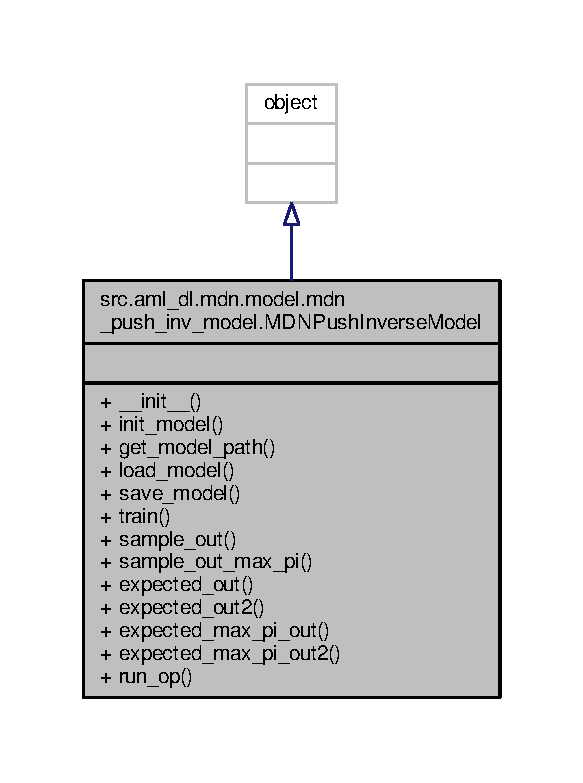
\includegraphics[width=283pt]{classsrc_1_1aml__dl_1_1mdn_1_1model_1_1mdn__push__inv__model_1_1_m_d_n_push_inverse_model__inherit__graph}
\end{center}
\end{figure}


Collaboration diagram for src.\+aml\+\_\+dl.\+mdn.\+model.\+mdn\+\_\+push\+\_\+inv\+\_\+model.\+M\+D\+N\+Push\+Inverse\+Model\+:
\nopagebreak
\begin{figure}[H]
\begin{center}
\leavevmode
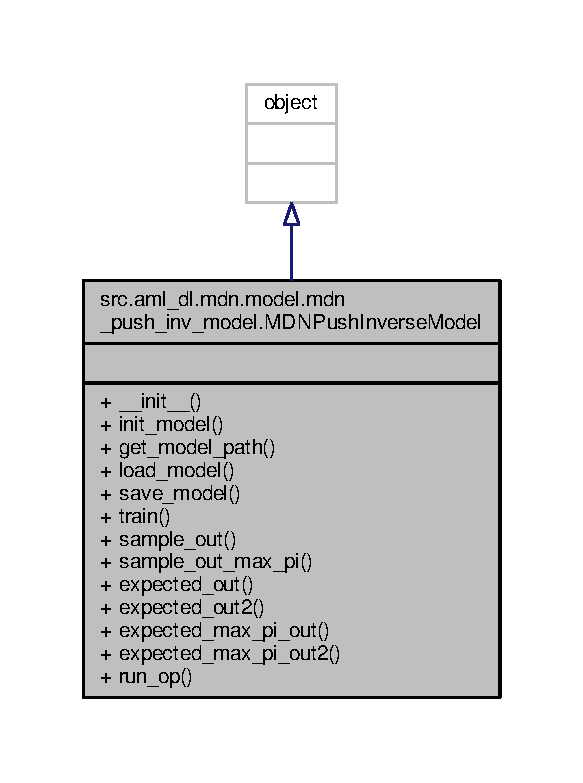
\includegraphics[width=283pt]{classsrc_1_1aml__dl_1_1mdn_1_1model_1_1mdn__push__inv__model_1_1_m_d_n_push_inverse_model__coll__graph}
\end{center}
\end{figure}
\subsection*{Public Member Functions}
\begin{DoxyCompactItemize}
\item 
\hypertarget{classsrc_1_1aml__dl_1_1mdn_1_1model_1_1mdn__push__inv__model_1_1_m_d_n_push_inverse_model_a3857d23d6d7b09814cbbef93a9b9940c}{}\label{classsrc_1_1aml__dl_1_1mdn_1_1model_1_1mdn__push__inv__model_1_1_m_d_n_push_inverse_model_a3857d23d6d7b09814cbbef93a9b9940c} 
def {\bfseries \+\_\+\+\_\+init\+\_\+\+\_\+} (self, sess, network\+\_\+params)
\item 
\hypertarget{classsrc_1_1aml__dl_1_1mdn_1_1model_1_1mdn__push__inv__model_1_1_m_d_n_push_inverse_model_a7aff8166ce747a753f7fdc368acc3c37}{}\label{classsrc_1_1aml__dl_1_1mdn_1_1model_1_1mdn__push__inv__model_1_1_m_d_n_push_inverse_model_a7aff8166ce747a753f7fdc368acc3c37} 
def {\bfseries init\+\_\+model} (self)
\item 
\hypertarget{classsrc_1_1aml__dl_1_1mdn_1_1model_1_1mdn__push__inv__model_1_1_m_d_n_push_inverse_model_a79f16a313aad5811cdbb58bcc193db1e}{}\label{classsrc_1_1aml__dl_1_1mdn_1_1model_1_1mdn__push__inv__model_1_1_m_d_n_push_inverse_model_a79f16a313aad5811cdbb58bcc193db1e} 
def {\bfseries get\+\_\+model\+\_\+path} (self)
\item 
\hypertarget{classsrc_1_1aml__dl_1_1mdn_1_1model_1_1mdn__push__inv__model_1_1_m_d_n_push_inverse_model_a1a95d39e8ef22f6c7930cab122ce0458}{}\label{classsrc_1_1aml__dl_1_1mdn_1_1model_1_1mdn__push__inv__model_1_1_m_d_n_push_inverse_model_a1a95d39e8ef22f6c7930cab122ce0458} 
def {\bfseries load\+\_\+model} (self)
\item 
\hypertarget{classsrc_1_1aml__dl_1_1mdn_1_1model_1_1mdn__push__inv__model_1_1_m_d_n_push_inverse_model_a78ec7bbea7e5afaeedd005586b700a86}{}\label{classsrc_1_1aml__dl_1_1mdn_1_1model_1_1mdn__push__inv__model_1_1_m_d_n_push_inverse_model_a78ec7bbea7e5afaeedd005586b700a86} 
def {\bfseries save\+\_\+model} (self)
\item 
\hypertarget{classsrc_1_1aml__dl_1_1mdn_1_1model_1_1mdn__push__inv__model_1_1_m_d_n_push_inverse_model_a158fa7524422abb2dde67957cb191680}{}\label{classsrc_1_1aml__dl_1_1mdn_1_1model_1_1mdn__push__inv__model_1_1_m_d_n_push_inverse_model_a158fa7524422abb2dde67957cb191680} 
def {\bfseries train} (self, x\+\_\+data, y\+\_\+data, epochs=10000)
\item 
\hypertarget{classsrc_1_1aml__dl_1_1mdn_1_1model_1_1mdn__push__inv__model_1_1_m_d_n_push_inverse_model_a714739d5cb44238925e462dd2f20017a}{}\label{classsrc_1_1aml__dl_1_1mdn_1_1model_1_1mdn__push__inv__model_1_1_m_d_n_push_inverse_model_a714739d5cb44238925e462dd2f20017a} 
def {\bfseries sample\+\_\+out} (self, x\+\_\+input, m\+\_\+samples=10)
\item 
\hypertarget{classsrc_1_1aml__dl_1_1mdn_1_1model_1_1mdn__push__inv__model_1_1_m_d_n_push_inverse_model_a2d4f64d96bebc2aa6728b6de026623c9}{}\label{classsrc_1_1aml__dl_1_1mdn_1_1model_1_1mdn__push__inv__model_1_1_m_d_n_push_inverse_model_a2d4f64d96bebc2aa6728b6de026623c9} 
def {\bfseries sample\+\_\+out\+\_\+max\+\_\+pi} (self, x\+\_\+input, m\+\_\+samples=10)
\item 
\hypertarget{classsrc_1_1aml__dl_1_1mdn_1_1model_1_1mdn__push__inv__model_1_1_m_d_n_push_inverse_model_af24b4f077df4aba9b40a26563b39ca44}{}\label{classsrc_1_1aml__dl_1_1mdn_1_1model_1_1mdn__push__inv__model_1_1_m_d_n_push_inverse_model_af24b4f077df4aba9b40a26563b39ca44} 
def {\bfseries expected\+\_\+out} (self, x\+\_\+input, m\+\_\+samples=10)
\item 
\hypertarget{classsrc_1_1aml__dl_1_1mdn_1_1model_1_1mdn__push__inv__model_1_1_m_d_n_push_inverse_model_a72bdc8d20fdd2dcfdc83eb363b465ef9}{}\label{classsrc_1_1aml__dl_1_1mdn_1_1model_1_1mdn__push__inv__model_1_1_m_d_n_push_inverse_model_a72bdc8d20fdd2dcfdc83eb363b465ef9} 
def {\bfseries expected\+\_\+out2} (self, x\+\_\+input, m\+\_\+samples=10)
\item 
\hypertarget{classsrc_1_1aml__dl_1_1mdn_1_1model_1_1mdn__push__inv__model_1_1_m_d_n_push_inverse_model_a041d9896a8ecafcf90b68e9d2694627a}{}\label{classsrc_1_1aml__dl_1_1mdn_1_1model_1_1mdn__push__inv__model_1_1_m_d_n_push_inverse_model_a041d9896a8ecafcf90b68e9d2694627a} 
def {\bfseries expected\+\_\+max\+\_\+pi\+\_\+out} (self, x\+\_\+input, m\+\_\+samples=10)
\item 
\hypertarget{classsrc_1_1aml__dl_1_1mdn_1_1model_1_1mdn__push__inv__model_1_1_m_d_n_push_inverse_model_a854d79e3467c5be8312d3a73ef0b75ec}{}\label{classsrc_1_1aml__dl_1_1mdn_1_1model_1_1mdn__push__inv__model_1_1_m_d_n_push_inverse_model_a854d79e3467c5be8312d3a73ef0b75ec} 
def {\bfseries expected\+\_\+max\+\_\+pi\+\_\+out2} (self, x\+\_\+input, m\+\_\+samples=10)
\item 
\hypertarget{classsrc_1_1aml__dl_1_1mdn_1_1model_1_1mdn__push__inv__model_1_1_m_d_n_push_inverse_model_a9ff89e2b0ea4275235cb7fd467dc2ab4}{}\label{classsrc_1_1aml__dl_1_1mdn_1_1model_1_1mdn__push__inv__model_1_1_m_d_n_push_inverse_model_a9ff89e2b0ea4275235cb7fd467dc2ab4} 
def {\bfseries run\+\_\+op} (self, op\+\_\+name, x\+\_\+input)
\end{DoxyCompactItemize}


The documentation for this class was generated from the following file\+:\begin{DoxyCompactItemize}
\item 
aml\+\_\+dl/src/aml\+\_\+dl/mdn/model/mdn\+\_\+push\+\_\+inv\+\_\+model.\+py\end{DoxyCompactItemize}

\hypertarget{classaml__ctrl_1_1utilities_1_1min__jerk__interp_1_1_min_jerk_interp}{}\section{aml\+\_\+ctrl.\+utilities.\+min\+\_\+jerk\+\_\+interp.\+Min\+Jerk\+Interp Class Reference}
\label{classaml__ctrl_1_1utilities_1_1min__jerk__interp_1_1_min_jerk_interp}\index{aml\+\_\+ctrl.\+utilities.\+min\+\_\+jerk\+\_\+interp.\+Min\+Jerk\+Interp@{aml\+\_\+ctrl.\+utilities.\+min\+\_\+jerk\+\_\+interp.\+Min\+Jerk\+Interp}}


Collaboration diagram for aml\+\_\+ctrl.\+utilities.\+min\+\_\+jerk\+\_\+interp.\+Min\+Jerk\+Interp\+:
\nopagebreak
\begin{figure}[H]
\begin{center}
\leavevmode
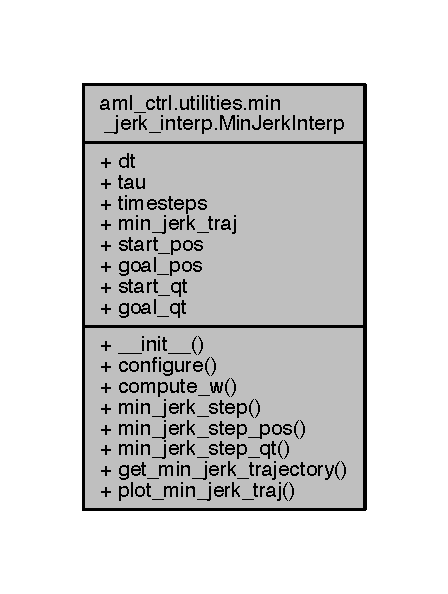
\includegraphics[width=215pt]{classaml__ctrl_1_1utilities_1_1min__jerk__interp_1_1_min_jerk_interp__coll__graph}
\end{center}
\end{figure}
\subsection*{Public Member Functions}
\begin{DoxyCompactItemize}
\item 
\hypertarget{classaml__ctrl_1_1utilities_1_1min__jerk__interp_1_1_min_jerk_interp_aadf63d0220915bfd457f26caaeedb52c}{}\label{classaml__ctrl_1_1utilities_1_1min__jerk__interp_1_1_min_jerk_interp_aadf63d0220915bfd457f26caaeedb52c} 
def {\bfseries \+\_\+\+\_\+init\+\_\+\+\_\+} (self, dt=0.\+05, tau=5.)
\item 
\hypertarget{classaml__ctrl_1_1utilities_1_1min__jerk__interp_1_1_min_jerk_interp_ad0948202cbfaeb4c69099e8ba32a5b09}{}\label{classaml__ctrl_1_1utilities_1_1min__jerk__interp_1_1_min_jerk_interp_ad0948202cbfaeb4c69099e8ba32a5b09} 
def {\bfseries configure} (self, start\+\_\+pos, start\+\_\+qt, goal\+\_\+pos, goal\+\_\+qt)
\item 
\hypertarget{classaml__ctrl_1_1utilities_1_1min__jerk__interp_1_1_min_jerk_interp_a84ec24d901c9582b4151de75b9b02b83}{}\label{classaml__ctrl_1_1utilities_1_1min__jerk__interp_1_1_min_jerk_interp_a84ec24d901c9582b4151de75b9b02b83} 
def {\bfseries compute\+\_\+w} (self, q, qdot)
\item 
\hypertarget{classaml__ctrl_1_1utilities_1_1min__jerk__interp_1_1_min_jerk_interp_a5620dafe71bfe0d1908dd810d01e846d}{}\label{classaml__ctrl_1_1utilities_1_1min__jerk__interp_1_1_min_jerk_interp_a5620dafe71bfe0d1908dd810d01e846d} 
def {\bfseries min\+\_\+jerk\+\_\+step} (self, x, xd, xdd, goal, tau)
\item 
\hypertarget{classaml__ctrl_1_1utilities_1_1min__jerk__interp_1_1_min_jerk_interp_a0c3279ef71e9e83355604f8c754ae5b7}{}\label{classaml__ctrl_1_1utilities_1_1min__jerk__interp_1_1_min_jerk_interp_a0c3279ef71e9e83355604f8c754ae5b7} 
def {\bfseries min\+\_\+jerk\+\_\+step\+\_\+pos} (self)
\item 
\hypertarget{classaml__ctrl_1_1utilities_1_1min__jerk__interp_1_1_min_jerk_interp_a5888e83ccea393d6775a684f44104489}{}\label{classaml__ctrl_1_1utilities_1_1min__jerk__interp_1_1_min_jerk_interp_a5888e83ccea393d6775a684f44104489} 
def {\bfseries min\+\_\+jerk\+\_\+step\+\_\+qt} (self)
\item 
\hypertarget{classaml__ctrl_1_1utilities_1_1min__jerk__interp_1_1_min_jerk_interp_a06e9332a4367aa9db11f4d3557a203c9}{}\label{classaml__ctrl_1_1utilities_1_1min__jerk__interp_1_1_min_jerk_interp_a06e9332a4367aa9db11f4d3557a203c9} 
def {\bfseries get\+\_\+min\+\_\+jerk\+\_\+trajectory} (self)
\item 
\hypertarget{classaml__ctrl_1_1utilities_1_1min__jerk__interp_1_1_min_jerk_interp_ab4470625eaf22769bdc5f20e914ad5dd}{}\label{classaml__ctrl_1_1utilities_1_1min__jerk__interp_1_1_min_jerk_interp_ab4470625eaf22769bdc5f20e914ad5dd} 
def {\bfseries plot\+\_\+min\+\_\+jerk\+\_\+traj} (self)
\end{DoxyCompactItemize}
\subsection*{Public Attributes}
\begin{DoxyCompactItemize}
\item 
\hypertarget{classaml__ctrl_1_1utilities_1_1min__jerk__interp_1_1_min_jerk_interp_a3cf50dd857ae275c6a9309c560a334f0}{}\label{classaml__ctrl_1_1utilities_1_1min__jerk__interp_1_1_min_jerk_interp_a3cf50dd857ae275c6a9309c560a334f0} 
{\bfseries dt}
\item 
\hypertarget{classaml__ctrl_1_1utilities_1_1min__jerk__interp_1_1_min_jerk_interp_abfbc4183bd40597d1f8ef549c8a954cd}{}\label{classaml__ctrl_1_1utilities_1_1min__jerk__interp_1_1_min_jerk_interp_abfbc4183bd40597d1f8ef549c8a954cd} 
{\bfseries tau}
\item 
\hypertarget{classaml__ctrl_1_1utilities_1_1min__jerk__interp_1_1_min_jerk_interp_a53f374cd9afb16fb0293c4f65987795d}{}\label{classaml__ctrl_1_1utilities_1_1min__jerk__interp_1_1_min_jerk_interp_a53f374cd9afb16fb0293c4f65987795d} 
{\bfseries timesteps}
\item 
\hypertarget{classaml__ctrl_1_1utilities_1_1min__jerk__interp_1_1_min_jerk_interp_a655ecaf3042fd23a9dea45fcac07c520}{}\label{classaml__ctrl_1_1utilities_1_1min__jerk__interp_1_1_min_jerk_interp_a655ecaf3042fd23a9dea45fcac07c520} 
{\bfseries min\+\_\+jerk\+\_\+traj}
\item 
\hypertarget{classaml__ctrl_1_1utilities_1_1min__jerk__interp_1_1_min_jerk_interp_a2154616a9adab36c591fc90b62ac66cc}{}\label{classaml__ctrl_1_1utilities_1_1min__jerk__interp_1_1_min_jerk_interp_a2154616a9adab36c591fc90b62ac66cc} 
{\bfseries start\+\_\+pos}
\item 
\hypertarget{classaml__ctrl_1_1utilities_1_1min__jerk__interp_1_1_min_jerk_interp_af33d73bed61d6eebe0ddbb1ca953a881}{}\label{classaml__ctrl_1_1utilities_1_1min__jerk__interp_1_1_min_jerk_interp_af33d73bed61d6eebe0ddbb1ca953a881} 
{\bfseries goal\+\_\+pos}
\item 
\hypertarget{classaml__ctrl_1_1utilities_1_1min__jerk__interp_1_1_min_jerk_interp_a1d7c1d1cc8b9b64922061d060d331d8a}{}\label{classaml__ctrl_1_1utilities_1_1min__jerk__interp_1_1_min_jerk_interp_a1d7c1d1cc8b9b64922061d060d331d8a} 
{\bfseries start\+\_\+qt}
\item 
\hypertarget{classaml__ctrl_1_1utilities_1_1min__jerk__interp_1_1_min_jerk_interp_a6aa537ca52a3e35e06ef582303e4501f}{}\label{classaml__ctrl_1_1utilities_1_1min__jerk__interp_1_1_min_jerk_interp_a6aa537ca52a3e35e06ef582303e4501f} 
{\bfseries goal\+\_\+qt}
\end{DoxyCompactItemize}


The documentation for this class was generated from the following file\+:\begin{DoxyCompactItemize}
\item 
aml\+\_\+robot/src/aml\+\_\+ctrl/utilities/min\+\_\+jerk\+\_\+interp.\+py\end{DoxyCompactItemize}

\hypertarget{classaml__robot_1_1mujoco_1_1mujoco__robot_1_1_mujoco_robot}{\section{aml\-\_\-robot.\-mujoco.\-mujoco\-\_\-robot.\-Mujoco\-Robot Class Reference}
\label{classaml__robot_1_1mujoco_1_1mujoco__robot_1_1_mujoco_robot}\index{aml\-\_\-robot.\-mujoco.\-mujoco\-\_\-robot.\-Mujoco\-Robot@{aml\-\_\-robot.\-mujoco.\-mujoco\-\_\-robot.\-Mujoco\-Robot}}
}


Collaboration diagram for aml\-\_\-robot.\-mujoco.\-mujoco\-\_\-robot.\-Mujoco\-Robot\-:
\nopagebreak
\begin{figure}[H]
\begin{center}
\leavevmode
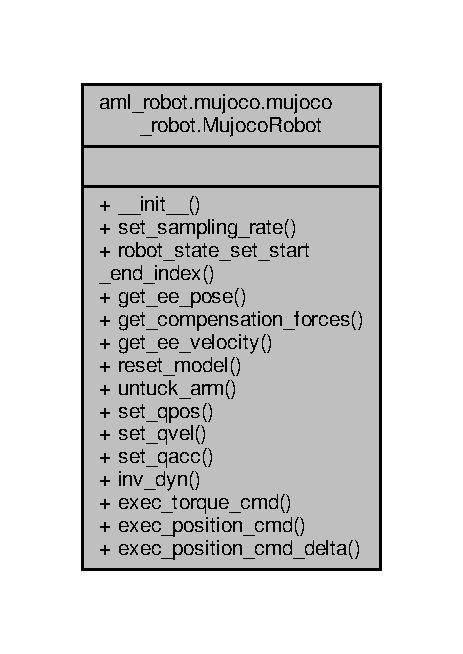
\includegraphics[width=222pt]{classaml__robot_1_1mujoco_1_1mujoco__robot_1_1_mujoco_robot__coll__graph}
\end{center}
\end{figure}
\subsection*{Public Member Functions}
\begin{DoxyCompactItemize}
\item 
\hypertarget{classaml__robot_1_1mujoco_1_1mujoco__robot_1_1_mujoco_robot_a3530563b849b9395adbd82dcdfc087ee}{def {\bfseries \-\_\-\-\_\-init\-\_\-\-\_\-}}\label{classaml__robot_1_1mujoco_1_1mujoco__robot_1_1_mujoco_robot_a3530563b849b9395adbd82dcdfc087ee}

\item 
\hypertarget{classaml__robot_1_1mujoco_1_1mujoco__robot_1_1_mujoco_robot_a7d63be2332de442538a71220c513edb7}{def {\bfseries set\-\_\-sampling\-\_\-rate}}\label{classaml__robot_1_1mujoco_1_1mujoco__robot_1_1_mujoco_robot_a7d63be2332de442538a71220c513edb7}

\item 
def \hyperlink{classaml__robot_1_1mujoco_1_1mujoco__robot_1_1_mujoco_robot_a196732855d5a685a8ef331f601411335}{robot\-\_\-state\-\_\-set\-\_\-start\-\_\-end\-\_\-index}
\item 
\hypertarget{classaml__robot_1_1mujoco_1_1mujoco__robot_1_1_mujoco_robot_aed5a762d049a169f35799364acb09b8e}{def {\bfseries get\-\_\-state}}\label{classaml__robot_1_1mujoco_1_1mujoco__robot_1_1_mujoco_robot_aed5a762d049a169f35799364acb09b8e}

\item 
\hypertarget{classaml__robot_1_1mujoco_1_1mujoco__robot_1_1_mujoco_robot_a7d56bde9444f10024c3e8efc721c9f8f}{def {\bfseries get\-\_\-ee\-\_\-pose}}\label{classaml__robot_1_1mujoco_1_1mujoco__robot_1_1_mujoco_robot_a7d56bde9444f10024c3e8efc721c9f8f}

\item 
\hypertarget{classaml__robot_1_1mujoco_1_1mujoco__robot_1_1_mujoco_robot_a7acbea899a6e19dd0544e7ed91c09b80}{def {\bfseries get\-\_\-compensation\-\_\-forces}}\label{classaml__robot_1_1mujoco_1_1mujoco__robot_1_1_mujoco_robot_a7acbea899a6e19dd0544e7ed91c09b80}

\item 
\hypertarget{classaml__robot_1_1mujoco_1_1mujoco__robot_1_1_mujoco_robot_ac368649b02e383db1de34378ae14066b}{def {\bfseries get\-\_\-ee\-\_\-velocity}}\label{classaml__robot_1_1mujoco_1_1mujoco__robot_1_1_mujoco_robot_ac368649b02e383db1de34378ae14066b}

\item 
\hypertarget{classaml__robot_1_1mujoco_1_1mujoco__robot_1_1_mujoco_robot_ae604beca2f4fc6a0ee451f48f6e62e44}{def {\bfseries reset\-\_\-model}}\label{classaml__robot_1_1mujoco_1_1mujoco__robot_1_1_mujoco_robot_ae604beca2f4fc6a0ee451f48f6e62e44}

\item 
\hypertarget{classaml__robot_1_1mujoco_1_1mujoco__robot_1_1_mujoco_robot_a1b6035deb34d6d23556fca80fed05f2f}{def {\bfseries untuck\-\_\-arm}}\label{classaml__robot_1_1mujoco_1_1mujoco__robot_1_1_mujoco_robot_a1b6035deb34d6d23556fca80fed05f2f}

\item 
\hypertarget{classaml__robot_1_1mujoco_1_1mujoco__robot_1_1_mujoco_robot_a879b704ca268878cb43f4179aa76b713}{def {\bfseries set\-\_\-qpos}}\label{classaml__robot_1_1mujoco_1_1mujoco__robot_1_1_mujoco_robot_a879b704ca268878cb43f4179aa76b713}

\item 
\hypertarget{classaml__robot_1_1mujoco_1_1mujoco__robot_1_1_mujoco_robot_a7270f56a4c8b3b05d43fc5a93e16690e}{def {\bfseries set\-\_\-qvel}}\label{classaml__robot_1_1mujoco_1_1mujoco__robot_1_1_mujoco_robot_a7270f56a4c8b3b05d43fc5a93e16690e}

\item 
\hypertarget{classaml__robot_1_1mujoco_1_1mujoco__robot_1_1_mujoco_robot_afe6b80c5eebad4523ee382cfffe8c42a}{def {\bfseries set\-\_\-qacc}}\label{classaml__robot_1_1mujoco_1_1mujoco__robot_1_1_mujoco_robot_afe6b80c5eebad4523ee382cfffe8c42a}

\item 
\hypertarget{classaml__robot_1_1mujoco_1_1mujoco__robot_1_1_mujoco_robot_a7f7654c35957ca875c923c79a8859d29}{def {\bfseries inv\-\_\-dyn}}\label{classaml__robot_1_1mujoco_1_1mujoco__robot_1_1_mujoco_robot_a7f7654c35957ca875c923c79a8859d29}

\item 
\hypertarget{classaml__robot_1_1mujoco_1_1mujoco__robot_1_1_mujoco_robot_a1f8a3036ae1750b6d3643522635da291}{def {\bfseries exec\-\_\-torque\-\_\-cmd}}\label{classaml__robot_1_1mujoco_1_1mujoco__robot_1_1_mujoco_robot_a1f8a3036ae1750b6d3643522635da291}

\item 
\hypertarget{classaml__robot_1_1mujoco_1_1mujoco__robot_1_1_mujoco_robot_a9859a0fb822385b998bde6f8a1f8ecd5}{def {\bfseries exec\-\_\-position\-\_\-cmd}}\label{classaml__robot_1_1mujoco_1_1mujoco__robot_1_1_mujoco_robot_a9859a0fb822385b998bde6f8a1f8ecd5}

\item 
\hypertarget{classaml__robot_1_1mujoco_1_1mujoco__robot_1_1_mujoco_robot_ac008821453a7c3453b86d9f23bc4e04b}{def {\bfseries exec\-\_\-position\-\_\-cmd\-\_\-delta}}\label{classaml__robot_1_1mujoco_1_1mujoco__robot_1_1_mujoco_robot_ac008821453a7c3453b86d9f23bc4e04b}

\end{DoxyCompactItemize}


\subsection{Member Function Documentation}
\hypertarget{classaml__robot_1_1mujoco_1_1mujoco__robot_1_1_mujoco_robot_a196732855d5a685a8ef331f601411335}{\index{aml\-\_\-robot\-::mujoco\-::mujoco\-\_\-robot\-::\-Mujoco\-Robot@{aml\-\_\-robot\-::mujoco\-::mujoco\-\_\-robot\-::\-Mujoco\-Robot}!robot\-\_\-state\-\_\-set\-\_\-start\-\_\-end\-\_\-index@{robot\-\_\-state\-\_\-set\-\_\-start\-\_\-end\-\_\-index}}
\index{robot\-\_\-state\-\_\-set\-\_\-start\-\_\-end\-\_\-index@{robot\-\_\-state\-\_\-set\-\_\-start\-\_\-end\-\_\-index}!aml_robot::mujoco::mujoco_robot::MujocoRobot@{aml\-\_\-robot\-::mujoco\-::mujoco\-\_\-robot\-::\-Mujoco\-Robot}}
\subsubsection[{robot\-\_\-state\-\_\-set\-\_\-start\-\_\-end\-\_\-index}]{\setlength{\rightskip}{0pt plus 5cm}def aml\-\_\-robot.\-mujoco.\-mujoco\-\_\-robot.\-Mujoco\-Robot.\-robot\-\_\-state\-\_\-set\-\_\-start\-\_\-end\-\_\-index (
\begin{DoxyParamCaption}
\item[{}]{self, }
\item[{}]{p\-\_\-start\-\_\-idx, }
\item[{}]{p\-\_\-end\-\_\-idx, }
\item[{}]{v\-\_\-start\-\_\-idx, }
\item[{}]{v\-\_\-end\-\_\-idx}
\end{DoxyParamCaption}
)}}\label{classaml__robot_1_1mujoco_1_1mujoco__robot_1_1_mujoco_robot_a196732855d5a685a8ef331f601411335}
\begin{DoxyVerb}since mujoco provides a single array of all states of all objects in the scene, it becomes essential
to give a start index and end index in that array which corresponds to the robot
if the input arguments are none, then all values are returned
\end{DoxyVerb}
 

The documentation for this class was generated from the following file\-:\begin{DoxyCompactItemize}
\item 
aml\-\_\-robot/src/aml\-\_\-robot/mujoco/mujoco\-\_\-robot.\-py\end{DoxyCompactItemize}

\hypertarget{classaml__robot_1_1mujoco_1_1mujoco__viewer_1_1_mujoco_viewer}{}\section{aml\+\_\+robot.\+mujoco.\+mujoco\+\_\+viewer.\+Mujoco\+Viewer Class Reference}
\label{classaml__robot_1_1mujoco_1_1mujoco__viewer_1_1_mujoco_viewer}\index{aml\+\_\+robot.\+mujoco.\+mujoco\+\_\+viewer.\+Mujoco\+Viewer@{aml\+\_\+robot.\+mujoco.\+mujoco\+\_\+viewer.\+Mujoco\+Viewer}}


Collaboration diagram for aml\+\_\+robot.\+mujoco.\+mujoco\+\_\+viewer.\+Mujoco\+Viewer\+:\nopagebreak
\begin{figure}[H]
\begin{center}
\leavevmode
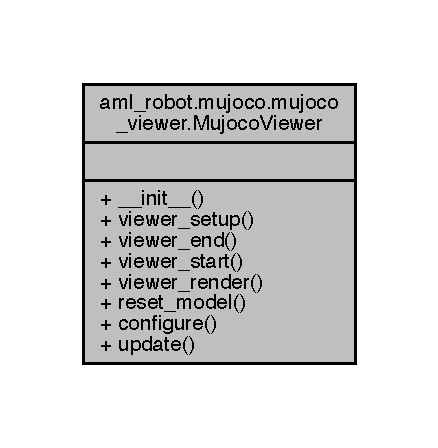
\includegraphics[width=210pt]{classaml__robot_1_1mujoco_1_1mujoco__viewer_1_1_mujoco_viewer__coll__graph}
\end{center}
\end{figure}
\subsection*{Public Member Functions}
\begin{DoxyCompactItemize}
\item 
\hypertarget{classaml__robot_1_1mujoco_1_1mujoco__viewer_1_1_mujoco_viewer_a930dba8e19b822639a9ab630d13d0e96}{}\label{classaml__robot_1_1mujoco_1_1mujoco__viewer_1_1_mujoco_viewer_a930dba8e19b822639a9ab630d13d0e96} 
def {\bfseries \+\_\+\+\_\+init\+\_\+\+\_\+} (self, mujoco\+\_\+robot, update\+\_\+rate=100)
\item 
\hypertarget{classaml__robot_1_1mujoco_1_1mujoco__viewer_1_1_mujoco_viewer_ab077677732577ea18dfeecdf1b4eb380}{}\label{classaml__robot_1_1mujoco_1_1mujoco__viewer_1_1_mujoco_viewer_ab077677732577ea18dfeecdf1b4eb380} 
def {\bfseries viewer\+\_\+setup} (self)
\item 
\hypertarget{classaml__robot_1_1mujoco_1_1mujoco__viewer_1_1_mujoco_viewer_ad19733ffbcfa3b0760655b1e2b1727c9}{}\label{classaml__robot_1_1mujoco_1_1mujoco__viewer_1_1_mujoco_viewer_ad19733ffbcfa3b0760655b1e2b1727c9} 
def {\bfseries viewer\+\_\+end} (self)
\item 
\hypertarget{classaml__robot_1_1mujoco_1_1mujoco__viewer_1_1_mujoco_viewer_a7973520f13f58e7e1056050dcef13a13}{}\label{classaml__robot_1_1mujoco_1_1mujoco__viewer_1_1_mujoco_viewer_a7973520f13f58e7e1056050dcef13a13} 
def {\bfseries viewer\+\_\+start} (self)
\item 
\hypertarget{classaml__robot_1_1mujoco_1_1mujoco__viewer_1_1_mujoco_viewer_a3515aa760e7f554fe77a8f3ceea3b7c8}{}\label{classaml__robot_1_1mujoco_1_1mujoco__viewer_1_1_mujoco_viewer_a3515aa760e7f554fe77a8f3ceea3b7c8} 
def {\bfseries viewer\+\_\+render} (self, mode=\textquotesingle{}human\textquotesingle{}, close=False)
\item 
\hypertarget{classaml__robot_1_1mujoco_1_1mujoco__viewer_1_1_mujoco_viewer_acbb6ddf0dde0b62b9a702d3fa71d643b}{}\label{classaml__robot_1_1mujoco_1_1mujoco__viewer_1_1_mujoco_viewer_acbb6ddf0dde0b62b9a702d3fa71d643b} 
def {\bfseries reset\+\_\+model} (self)
\item 
\hypertarget{classaml__robot_1_1mujoco_1_1mujoco__viewer_1_1_mujoco_viewer_af49847f19382cfdbd9e2e633e09efcda}{}\label{classaml__robot_1_1mujoco_1_1mujoco__viewer_1_1_mujoco_viewer_af49847f19382cfdbd9e2e633e09efcda} 
def {\bfseries configure} (self)
\item 
\hypertarget{classaml__robot_1_1mujoco_1_1mujoco__viewer_1_1_mujoco_viewer_a60de01cc08fbf120359e8e6070f9eb8e}{}\label{classaml__robot_1_1mujoco_1_1mujoco__viewer_1_1_mujoco_viewer_a60de01cc08fbf120359e8e6070f9eb8e} 
def {\bfseries update} (self, event)
\end{DoxyCompactItemize}


The documentation for this class was generated from the following file\+:\begin{DoxyCompactItemize}
\item 
aml\+\_\+robot/src/aml\+\_\+robot/mujoco/mujoco\+\_\+viewer.\+py\end{DoxyCompactItemize}

\hypertarget{classaml__ctrl_1_1controllers_1_1os__controllers_1_1os__bi__arm__controller_1_1_o_s_bi_arm_controller}{\section{aml\-\_\-ctrl.\-controllers.\-os\-\_\-controllers.\-os\-\_\-bi\-\_\-arm\-\_\-controller.\-O\-S\-Bi\-Arm\-Controller Class Reference}
\label{classaml__ctrl_1_1controllers_1_1os__controllers_1_1os__bi__arm__controller_1_1_o_s_bi_arm_controller}\index{aml\-\_\-ctrl.\-controllers.\-os\-\_\-controllers.\-os\-\_\-bi\-\_\-arm\-\_\-controller.\-O\-S\-Bi\-Arm\-Controller@{aml\-\_\-ctrl.\-controllers.\-os\-\_\-controllers.\-os\-\_\-bi\-\_\-arm\-\_\-controller.\-O\-S\-Bi\-Arm\-Controller}}
}


Inheritance diagram for aml\-\_\-ctrl.\-controllers.\-os\-\_\-controllers.\-os\-\_\-bi\-\_\-arm\-\_\-controller.\-O\-S\-Bi\-Arm\-Controller\-:
\nopagebreak
\begin{figure}[H]
\begin{center}
\leavevmode
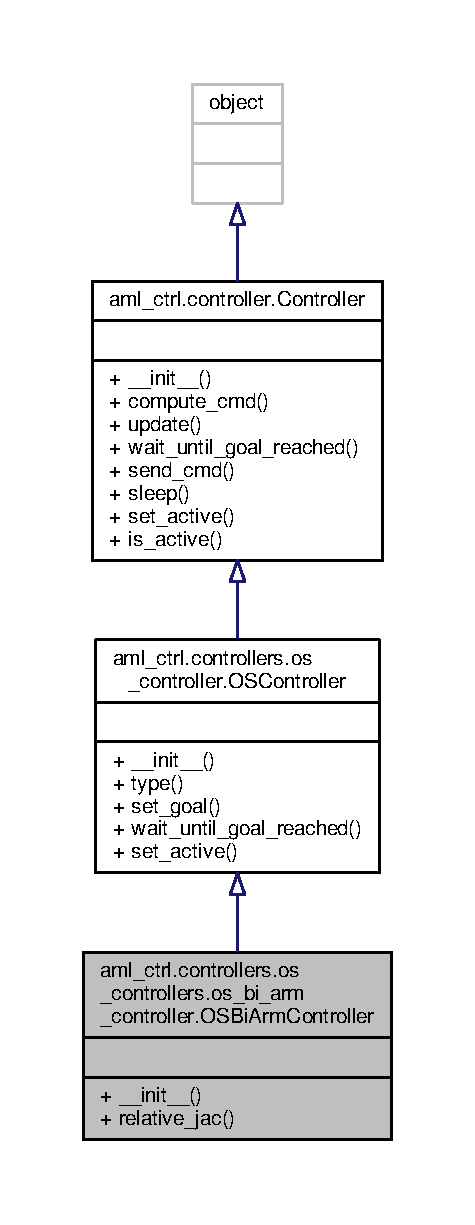
\includegraphics[height=550pt]{classaml__ctrl_1_1controllers_1_1os__controllers_1_1os__bi__arm__controller_1_1_o_s_bi_arm_controller__inherit__graph}
\end{center}
\end{figure}


Collaboration diagram for aml\-\_\-ctrl.\-controllers.\-os\-\_\-controllers.\-os\-\_\-bi\-\_\-arm\-\_\-controller.\-O\-S\-Bi\-Arm\-Controller\-:
\nopagebreak
\begin{figure}[H]
\begin{center}
\leavevmode
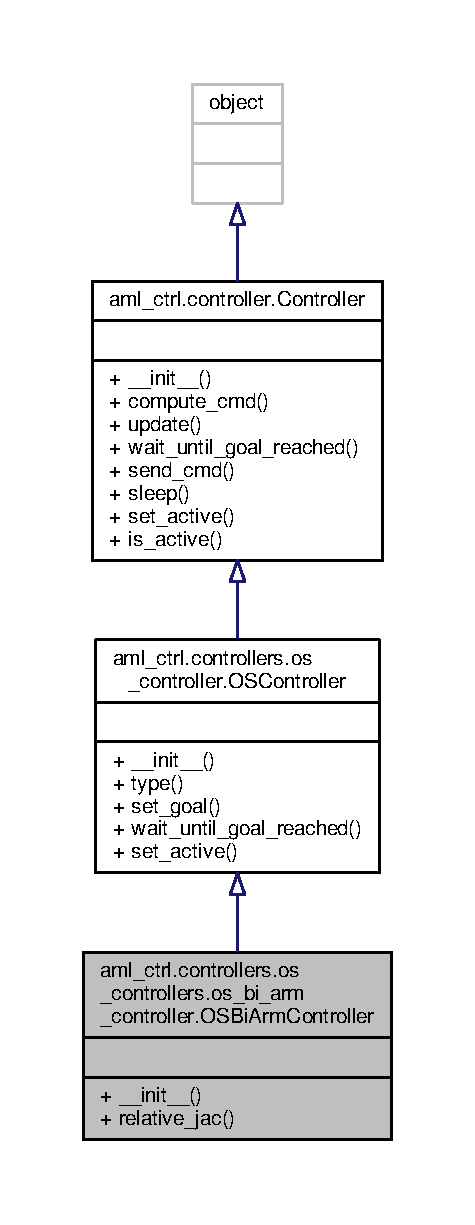
\includegraphics[height=550pt]{classaml__ctrl_1_1controllers_1_1os__controllers_1_1os__bi__arm__controller_1_1_o_s_bi_arm_controller__coll__graph}
\end{center}
\end{figure}
\subsection*{Public Member Functions}
\begin{DoxyCompactItemize}
\item 
\hypertarget{classaml__ctrl_1_1controllers_1_1os__controllers_1_1os__bi__arm__controller_1_1_o_s_bi_arm_controller_a9800c28c617d6748e1e1b78ee3ccc549}{def {\bfseries \-\_\-\-\_\-init\-\_\-\-\_\-}}\label{classaml__ctrl_1_1controllers_1_1os__controllers_1_1os__bi__arm__controller_1_1_o_s_bi_arm_controller_a9800c28c617d6748e1e1b78ee3ccc549}

\item 
\hypertarget{classaml__ctrl_1_1controllers_1_1os__controllers_1_1os__bi__arm__controller_1_1_o_s_bi_arm_controller_ac3e3ec1e8bcf59e02f632ed5ae5ea048}{def {\bfseries relative\-\_\-jac}}\label{classaml__ctrl_1_1controllers_1_1os__controllers_1_1os__bi__arm__controller_1_1_o_s_bi_arm_controller_ac3e3ec1e8bcf59e02f632ed5ae5ea048}

\end{DoxyCompactItemize}


The documentation for this class was generated from the following file\-:\begin{DoxyCompactItemize}
\item 
aml\-\_\-ctrl/src/aml\-\_\-ctrl/controllers/os\-\_\-controllers/os\-\_\-bi\-\_\-arm\-\_\-controller.\-py\end{DoxyCompactItemize}

\hypertarget{classaml__ctrl_1_1controllers_1_1os__controller_1_1_o_s_controller}{\section{aml\-\_\-ctrl.\-controllers.\-os\-\_\-controller.\-O\-S\-Controller Class Reference}
\label{classaml__ctrl_1_1controllers_1_1os__controller_1_1_o_s_controller}\index{aml\-\_\-ctrl.\-controllers.\-os\-\_\-controller.\-O\-S\-Controller@{aml\-\_\-ctrl.\-controllers.\-os\-\_\-controller.\-O\-S\-Controller}}
}


Inheritance diagram for aml\-\_\-ctrl.\-controllers.\-os\-\_\-controller.\-O\-S\-Controller\-:
\nopagebreak
\begin{figure}[H]
\begin{center}
\leavevmode
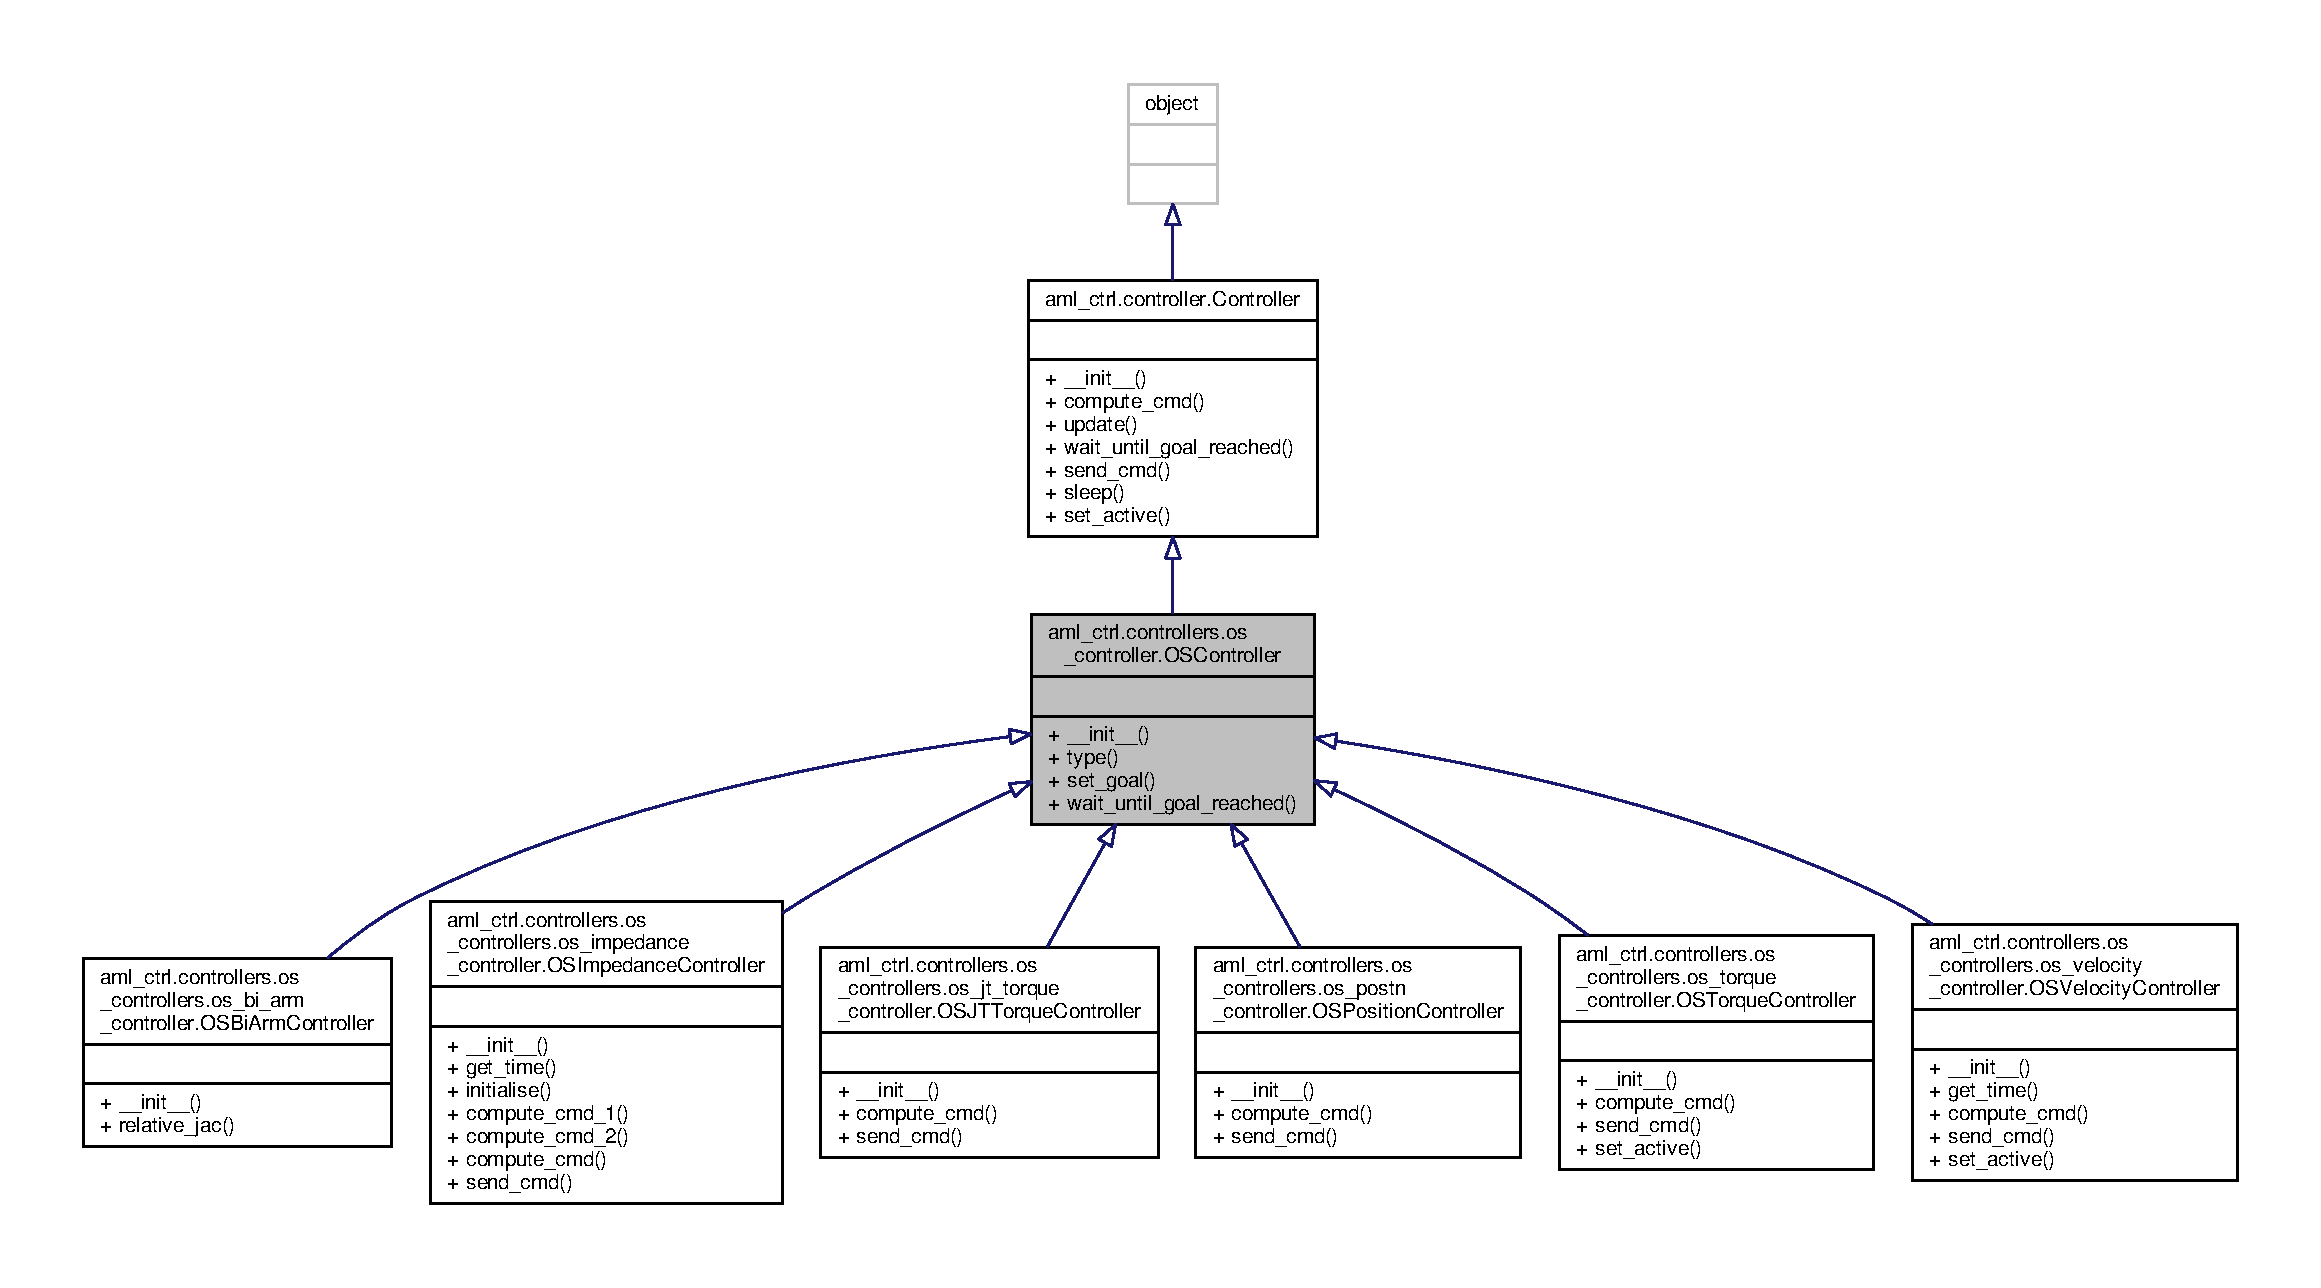
\includegraphics[width=350pt]{classaml__ctrl_1_1controllers_1_1os__controller_1_1_o_s_controller__inherit__graph}
\end{center}
\end{figure}


Collaboration diagram for aml\-\_\-ctrl.\-controllers.\-os\-\_\-controller.\-O\-S\-Controller\-:
\nopagebreak
\begin{figure}[H]
\begin{center}
\leavevmode
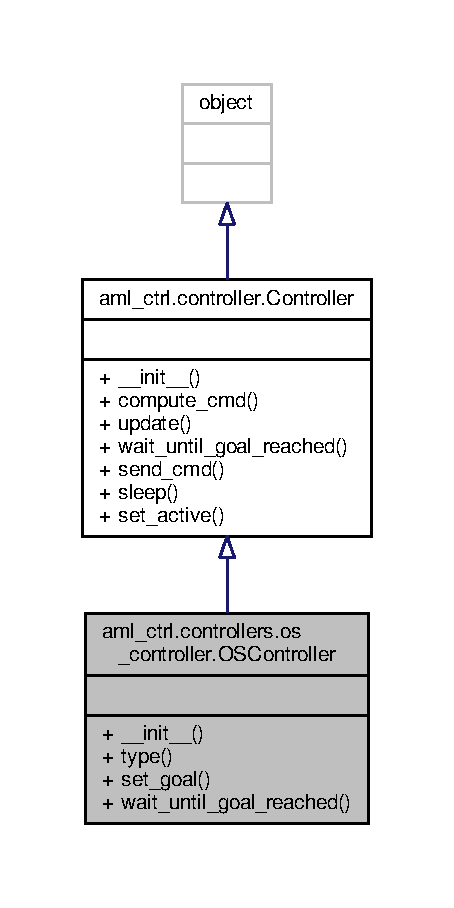
\includegraphics[width=218pt]{classaml__ctrl_1_1controllers_1_1os__controller_1_1_o_s_controller__coll__graph}
\end{center}
\end{figure}
\subsection*{Public Member Functions}
\begin{DoxyCompactItemize}
\item 
\hypertarget{classaml__ctrl_1_1controllers_1_1os__controller_1_1_o_s_controller_a45df7c8506ac273fa1fa4151d150bce6}{def {\bfseries \-\_\-\-\_\-init\-\_\-\-\_\-}}\label{classaml__ctrl_1_1controllers_1_1os__controller_1_1_o_s_controller_a45df7c8506ac273fa1fa4151d150bce6}

\item 
\hypertarget{classaml__ctrl_1_1controllers_1_1os__controller_1_1_o_s_controller_abfe6dd54b6461dfeedfec2d38c77f471}{def {\bfseries type}}\label{classaml__ctrl_1_1controllers_1_1os__controller_1_1_o_s_controller_abfe6dd54b6461dfeedfec2d38c77f471}

\item 
\hypertarget{classaml__ctrl_1_1controllers_1_1os__controller_1_1_o_s_controller_ac69f3c28e16ac763aa1368b8d8fb08ae}{def {\bfseries set\-\_\-goal}}\label{classaml__ctrl_1_1controllers_1_1os__controller_1_1_o_s_controller_ac69f3c28e16ac763aa1368b8d8fb08ae}

\item 
\hypertarget{classaml__ctrl_1_1controllers_1_1os__controller_1_1_o_s_controller_afbb13642219c803856fb69f8104e97fe}{def {\bfseries wait\-\_\-until\-\_\-goal\-\_\-reached}}\label{classaml__ctrl_1_1controllers_1_1os__controller_1_1_o_s_controller_afbb13642219c803856fb69f8104e97fe}

\item 
\hypertarget{classaml__ctrl_1_1controllers_1_1os__controller_1_1_o_s_controller_a84a896972570094acab46363b2338b1a}{def {\bfseries set\-\_\-active}}\label{classaml__ctrl_1_1controllers_1_1os__controller_1_1_o_s_controller_a84a896972570094acab46363b2338b1a}

\end{DoxyCompactItemize}


The documentation for this class was generated from the following file\-:\begin{DoxyCompactItemize}
\item 
aml\-\_\-ctrl/src/aml\-\_\-ctrl/controllers/os\-\_\-controller.\-py\end{DoxyCompactItemize}

\hypertarget{classaml__ctrl_1_1controllers_1_1os__controllers_1_1os__jt__torque__controller_1_1_o_s_j_t_torque_controller}{}\section{aml\+\_\+ctrl.\+controllers.\+os\+\_\+controllers.\+os\+\_\+jt\+\_\+torque\+\_\+controller.\+O\+S\+J\+T\+Torque\+Controller Class Reference}
\label{classaml__ctrl_1_1controllers_1_1os__controllers_1_1os__jt__torque__controller_1_1_o_s_j_t_torque_controller}\index{aml\+\_\+ctrl.\+controllers.\+os\+\_\+controllers.\+os\+\_\+jt\+\_\+torque\+\_\+controller.\+O\+S\+J\+T\+Torque\+Controller@{aml\+\_\+ctrl.\+controllers.\+os\+\_\+controllers.\+os\+\_\+jt\+\_\+torque\+\_\+controller.\+O\+S\+J\+T\+Torque\+Controller}}


Inheritance diagram for aml\+\_\+ctrl.\+controllers.\+os\+\_\+controllers.\+os\+\_\+jt\+\_\+torque\+\_\+controller.\+O\+S\+J\+T\+Torque\+Controller\+:\nopagebreak
\begin{figure}[H]
\begin{center}
\leavevmode
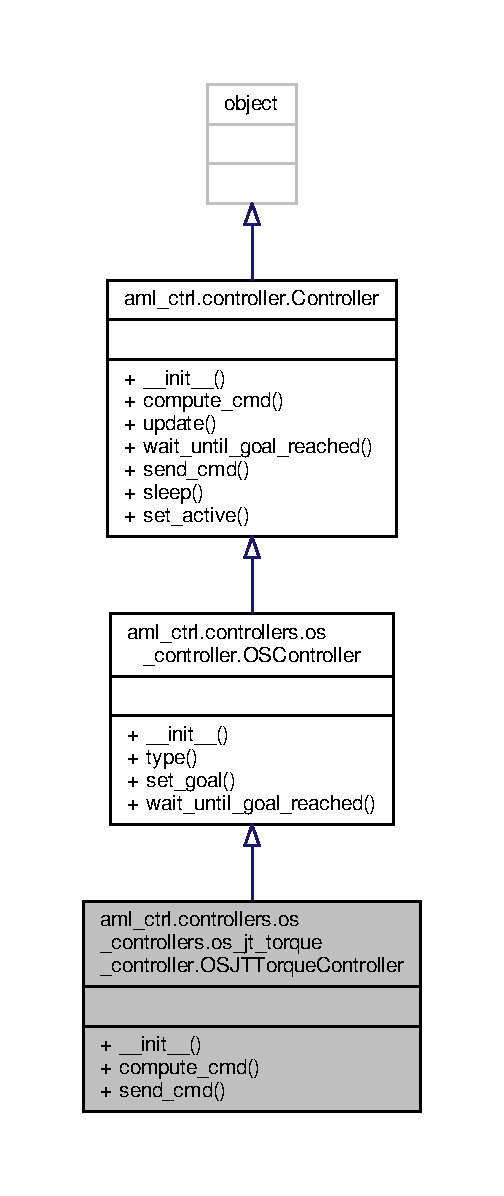
\includegraphics[width=244pt]{classaml__ctrl_1_1controllers_1_1os__controllers_1_1os__jt__torque__controller_1_1_o_s_j_t_torque_controller__inherit__graph}
\end{center}
\end{figure}


Collaboration diagram for aml\+\_\+ctrl.\+controllers.\+os\+\_\+controllers.\+os\+\_\+jt\+\_\+torque\+\_\+controller.\+O\+S\+J\+T\+Torque\+Controller\+:\nopagebreak
\begin{figure}[H]
\begin{center}
\leavevmode
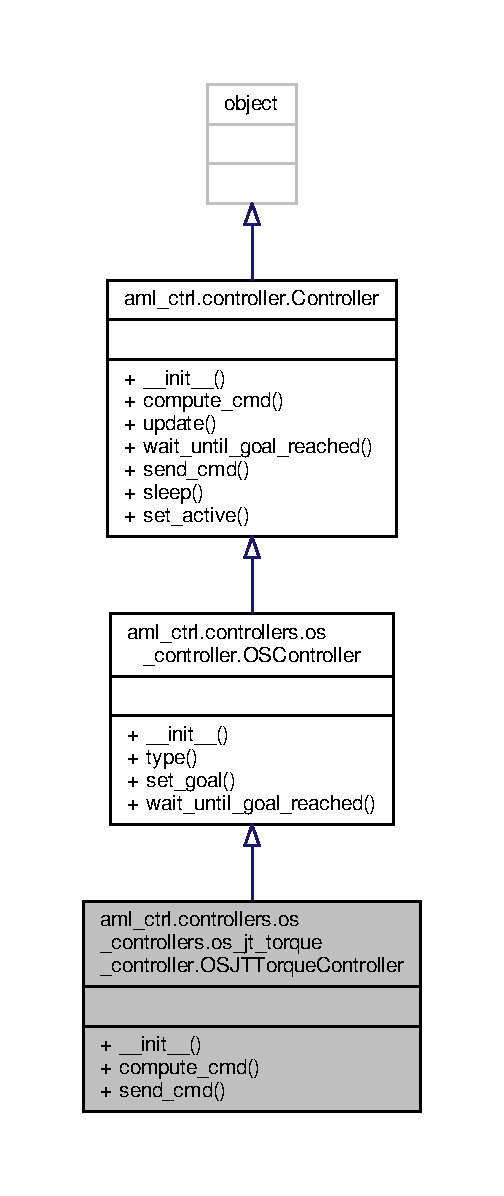
\includegraphics[width=244pt]{classaml__ctrl_1_1controllers_1_1os__controllers_1_1os__jt__torque__controller_1_1_o_s_j_t_torque_controller__coll__graph}
\end{center}
\end{figure}
\subsection*{Public Member Functions}
\begin{DoxyCompactItemize}
\item 
\hypertarget{classaml__ctrl_1_1controllers_1_1os__controllers_1_1os__jt__torque__controller_1_1_o_s_j_t_torque_controller_a6a9057f3af216e5baffb06f788cb3a7a}{}\label{classaml__ctrl_1_1controllers_1_1os__controllers_1_1os__jt__torque__controller_1_1_o_s_j_t_torque_controller_a6a9057f3af216e5baffb06f788cb3a7a} 
def {\bfseries \+\_\+\+\_\+init\+\_\+\+\_\+} (self, robot\+\_\+interface, config=O\+S\+\_\+\+J\+T\+\_\+\+T\+O\+R\+Q\+U\+E\+\_\+\+C\+N\+T\+LR)
\item 
\hypertarget{classaml__ctrl_1_1controllers_1_1os__controllers_1_1os__jt__torque__controller_1_1_o_s_j_t_torque_controller_ae53a96d9c5ad714a5f2bd8e7584093e7}{}\label{classaml__ctrl_1_1controllers_1_1os__controllers_1_1os__jt__torque__controller_1_1_o_s_j_t_torque_controller_ae53a96d9c5ad714a5f2bd8e7584093e7} 
def {\bfseries compute\+\_\+cmd} (self, time\+\_\+elapsed)
\item 
\hypertarget{classaml__ctrl_1_1controllers_1_1os__controllers_1_1os__jt__torque__controller_1_1_o_s_j_t_torque_controller_afe7e4b35075932fbaac675595bc94e55}{}\label{classaml__ctrl_1_1controllers_1_1os__controllers_1_1os__jt__torque__controller_1_1_o_s_j_t_torque_controller_afe7e4b35075932fbaac675595bc94e55} 
def {\bfseries send\+\_\+cmd} (self, time\+\_\+elapsed)
\end{DoxyCompactItemize}


The documentation for this class was generated from the following file\+:\begin{DoxyCompactItemize}
\item 
aml\+\_\+ctrl/src/aml\+\_\+ctrl/controllers/os\+\_\+controllers/os\+\_\+jt\+\_\+torque\+\_\+controller.\+py\end{DoxyCompactItemize}

\hypertarget{classaml__ctrl_1_1controllers_1_1os__controllers_1_1os__postn__controller_1_1_o_s_position_controller}{\section{aml\-\_\-ctrl.\-controllers.\-os\-\_\-controllers.\-os\-\_\-postn\-\_\-controller.\-O\-S\-Position\-Controller Class Reference}
\label{classaml__ctrl_1_1controllers_1_1os__controllers_1_1os__postn__controller_1_1_o_s_position_controller}\index{aml\-\_\-ctrl.\-controllers.\-os\-\_\-controllers.\-os\-\_\-postn\-\_\-controller.\-O\-S\-Position\-Controller@{aml\-\_\-ctrl.\-controllers.\-os\-\_\-controllers.\-os\-\_\-postn\-\_\-controller.\-O\-S\-Position\-Controller}}
}


Inheritance diagram for aml\-\_\-ctrl.\-controllers.\-os\-\_\-controllers.\-os\-\_\-postn\-\_\-controller.\-O\-S\-Position\-Controller\-:
\nopagebreak
\begin{figure}[H]
\begin{center}
\leavevmode
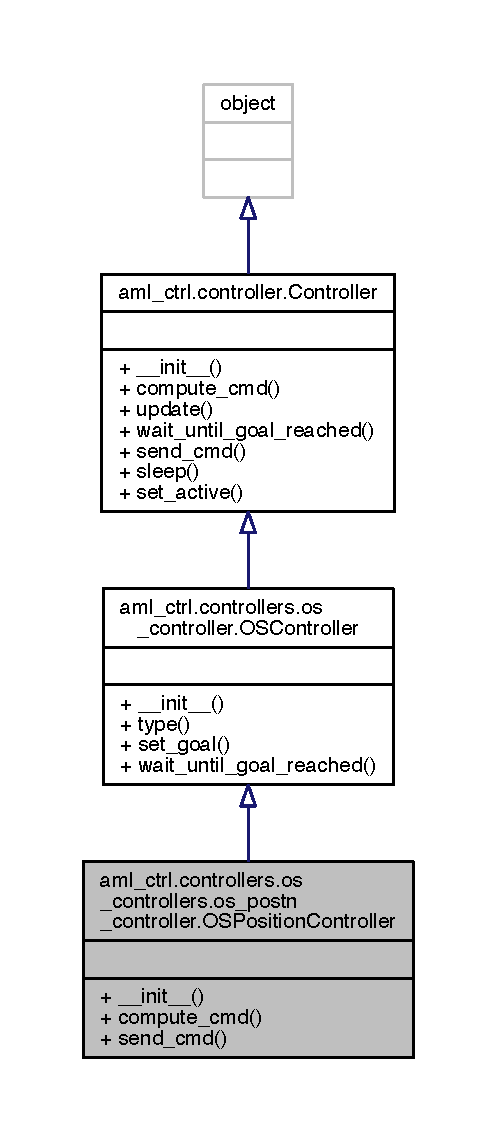
\includegraphics[height=550pt]{classaml__ctrl_1_1controllers_1_1os__controllers_1_1os__postn__controller_1_1_o_s_position_controller__inherit__graph}
\end{center}
\end{figure}


Collaboration diagram for aml\-\_\-ctrl.\-controllers.\-os\-\_\-controllers.\-os\-\_\-postn\-\_\-controller.\-O\-S\-Position\-Controller\-:
\nopagebreak
\begin{figure}[H]
\begin{center}
\leavevmode
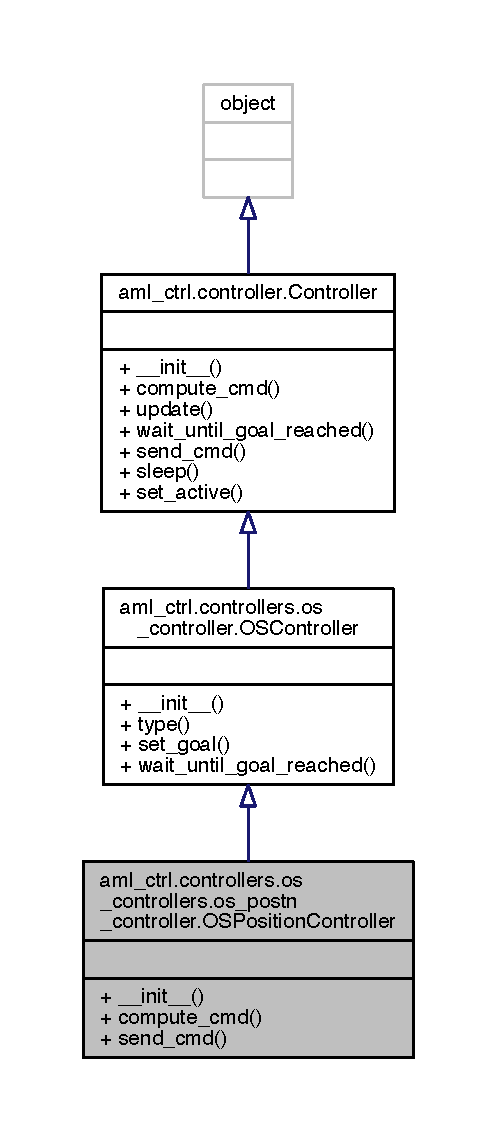
\includegraphics[height=550pt]{classaml__ctrl_1_1controllers_1_1os__controllers_1_1os__postn__controller_1_1_o_s_position_controller__coll__graph}
\end{center}
\end{figure}
\subsection*{Public Member Functions}
\begin{DoxyCompactItemize}
\item 
def \hyperlink{classaml__ctrl_1_1controllers_1_1os__controllers_1_1os__postn__controller_1_1_o_s_position_controller_a4ef9b21568a648b97bcd2fbf1781055a}{\-\_\-\-\_\-init\-\_\-\-\_\-}
\item 
\hypertarget{classaml__ctrl_1_1controllers_1_1os__controllers_1_1os__postn__controller_1_1_o_s_position_controller_a2dfdbc0052a9e76beebe4f265cb6b47d}{def {\bfseries compute\-\_\-cmd}}\label{classaml__ctrl_1_1controllers_1_1os__controllers_1_1os__postn__controller_1_1_o_s_position_controller_a2dfdbc0052a9e76beebe4f265cb6b47d}

\item 
\hypertarget{classaml__ctrl_1_1controllers_1_1os__controllers_1_1os__postn__controller_1_1_o_s_position_controller_a5ab45b868042fa13b9a38e785e8b5d6b}{def {\bfseries send\-\_\-cmd}}\label{classaml__ctrl_1_1controllers_1_1os__controllers_1_1os__postn__controller_1_1_o_s_position_controller_a5ab45b868042fa13b9a38e785e8b5d6b}

\end{DoxyCompactItemize}


\subsection{Detailed Description}
\begin{DoxyVerb}This class is an implementation fo the Operational Space position control
The type of control scheme is given in Robotics: Modelling, Planning and Control (page: 345)
Some equation of this is also adpated from http://journals.sagepub.com/doi/abs/10.1177/0278364908091463
Paper title : Operational Space Control: A Theoretical and Empirical Comparison
This code control scheme it is assumed to have an already gravity compensated arm
i.e. the gravity compensation happens in the joint space, while the operation space is used for task control
\end{DoxyVerb}
 

\subsection{Constructor \& Destructor Documentation}
\hypertarget{classaml__ctrl_1_1controllers_1_1os__controllers_1_1os__postn__controller_1_1_o_s_position_controller_a4ef9b21568a648b97bcd2fbf1781055a}{\index{aml\-\_\-ctrl\-::controllers\-::os\-\_\-controllers\-::os\-\_\-postn\-\_\-controller\-::\-O\-S\-Position\-Controller@{aml\-\_\-ctrl\-::controllers\-::os\-\_\-controllers\-::os\-\_\-postn\-\_\-controller\-::\-O\-S\-Position\-Controller}!\-\_\-\-\_\-init\-\_\-\-\_\-@{\-\_\-\-\_\-init\-\_\-\-\_\-}}
\index{\-\_\-\-\_\-init\-\_\-\-\_\-@{\-\_\-\-\_\-init\-\_\-\-\_\-}!aml_ctrl::controllers::os_controllers::os_postn_controller::OSPositionController@{aml\-\_\-ctrl\-::controllers\-::os\-\_\-controllers\-::os\-\_\-postn\-\_\-controller\-::\-O\-S\-Position\-Controller}}
\subsubsection[{\-\_\-\-\_\-init\-\_\-\-\_\-}]{\setlength{\rightskip}{0pt plus 5cm}def aml\-\_\-ctrl.\-controllers.\-os\-\_\-controllers.\-os\-\_\-postn\-\_\-controller.\-O\-S\-Position\-Controller.\-\_\-\-\_\-init\-\_\-\-\_\- (
\begin{DoxyParamCaption}
\item[{}]{self, }
\item[{}]{robot\-\_\-interface, }
\item[{}]{config = {\ttfamily OS\-\_\-POSTN\-\_\-CNTLR}}
\end{DoxyParamCaption}
)}}\label{classaml__ctrl_1_1controllers_1_1os__controllers_1_1os__postn__controller_1_1_o_s_position_controller_a4ef9b21568a648b97bcd2fbf1781055a}
\begin{DoxyVerb}Constructor of the class,
Args:
robot_interface : interface to the arm (type: aml_robot)
config: params: 
        kp_p : proportional gain for position
        kd_p : derivative gain for position
        kp_o : proportional gain for orientation
        kd_o : derivative gain for orientation
        null_kp: proportional gain for null space controller
        null_kd: derivative gain for null space controller
        alpha: null space control mixing factor
        rate: rate of speed sending commands
        dt: time step
\end{DoxyVerb}
 

The documentation for this class was generated from the following file\-:\begin{DoxyCompactItemize}
\item 
aml\-\_\-ctrl/src/aml\-\_\-ctrl/controllers/os\-\_\-controllers/os\-\_\-postn\-\_\-controller.\-py\end{DoxyCompactItemize}

\hypertarget{classaml__ctrl_1_1controllers_1_1os__controllers_1_1os__torque__controller_1_1_o_s_torque_controller}{\section{aml\-\_\-ctrl.\-controllers.\-os\-\_\-controllers.\-os\-\_\-torque\-\_\-controller.\-O\-S\-Torque\-Controller Class Reference}
\label{classaml__ctrl_1_1controllers_1_1os__controllers_1_1os__torque__controller_1_1_o_s_torque_controller}\index{aml\-\_\-ctrl.\-controllers.\-os\-\_\-controllers.\-os\-\_\-torque\-\_\-controller.\-O\-S\-Torque\-Controller@{aml\-\_\-ctrl.\-controllers.\-os\-\_\-controllers.\-os\-\_\-torque\-\_\-controller.\-O\-S\-Torque\-Controller}}
}


Inheritance diagram for aml\-\_\-ctrl.\-controllers.\-os\-\_\-controllers.\-os\-\_\-torque\-\_\-controller.\-O\-S\-Torque\-Controller\-:
\nopagebreak
\begin{figure}[H]
\begin{center}
\leavevmode
\includegraphics[height=550pt]{classaml__ctrl_1_1controllers_1_1os__controllers_1_1os__torque__controller_1_1_o_s_torque_controller__inherit__graph}
\end{center}
\end{figure}


Collaboration diagram for aml\-\_\-ctrl.\-controllers.\-os\-\_\-controllers.\-os\-\_\-torque\-\_\-controller.\-O\-S\-Torque\-Controller\-:
\nopagebreak
\begin{figure}[H]
\begin{center}
\leavevmode
\includegraphics[height=550pt]{classaml__ctrl_1_1controllers_1_1os__controllers_1_1os__torque__controller_1_1_o_s_torque_controller__coll__graph}
\end{center}
\end{figure}
\subsection*{Public Member Functions}
\begin{DoxyCompactItemize}
\item 
def \hyperlink{classaml__ctrl_1_1controllers_1_1os__controllers_1_1os__torque__controller_1_1_o_s_torque_controller_ac1608a2c52270e0612e0c86bf7d1c205}{\-\_\-\-\_\-init\-\_\-\-\_\-}
\item 
\hypertarget{classaml__ctrl_1_1controllers_1_1os__controllers_1_1os__torque__controller_1_1_o_s_torque_controller_ade8dd018b7bb2e5106b154b36948d8d1}{def {\bfseries compute\-\_\-cmd}}\label{classaml__ctrl_1_1controllers_1_1os__controllers_1_1os__torque__controller_1_1_o_s_torque_controller_ade8dd018b7bb2e5106b154b36948d8d1}

\item 
\hypertarget{classaml__ctrl_1_1controllers_1_1os__controllers_1_1os__torque__controller_1_1_o_s_torque_controller_a31d3e8ae8563a5f31b173d87eafaa996}{def {\bfseries send\-\_\-cmd}}\label{classaml__ctrl_1_1controllers_1_1os__controllers_1_1os__torque__controller_1_1_o_s_torque_controller_a31d3e8ae8563a5f31b173d87eafaa996}

\item 
\hypertarget{classaml__ctrl_1_1controllers_1_1os__controllers_1_1os__torque__controller_1_1_o_s_torque_controller_a73b83e3fd7cfaead53fa8287766f7d61}{def {\bfseries set\-\_\-active}}\label{classaml__ctrl_1_1controllers_1_1os__controllers_1_1os__torque__controller_1_1_o_s_torque_controller_a73b83e3fd7cfaead53fa8287766f7d61}

\end{DoxyCompactItemize}


\subsection{Detailed Description}
\begin{DoxyVerb}This class is an implementation fo the Operational Space velocity control 
controller specified in http://journals.sagepub.com/doi/abs/10.1177/0278364908091463
Paper title : Operational Space Control: A Theoretical and Empirical Comparison (section 3.1)
This code control scheme it is assumed to have an already gravity compensated arm
i.e. the gravity compensation happens in the joint space, while the operation space is used for task control
\end{DoxyVerb}
 

\subsection{Constructor \& Destructor Documentation}
\hypertarget{classaml__ctrl_1_1controllers_1_1os__controllers_1_1os__torque__controller_1_1_o_s_torque_controller_ac1608a2c52270e0612e0c86bf7d1c205}{\index{aml\-\_\-ctrl\-::controllers\-::os\-\_\-controllers\-::os\-\_\-torque\-\_\-controller\-::\-O\-S\-Torque\-Controller@{aml\-\_\-ctrl\-::controllers\-::os\-\_\-controllers\-::os\-\_\-torque\-\_\-controller\-::\-O\-S\-Torque\-Controller}!\-\_\-\-\_\-init\-\_\-\-\_\-@{\-\_\-\-\_\-init\-\_\-\-\_\-}}
\index{\-\_\-\-\_\-init\-\_\-\-\_\-@{\-\_\-\-\_\-init\-\_\-\-\_\-}!aml_ctrl::controllers::os_controllers::os_torque_controller::OSTorqueController@{aml\-\_\-ctrl\-::controllers\-::os\-\_\-controllers\-::os\-\_\-torque\-\_\-controller\-::\-O\-S\-Torque\-Controller}}
\subsubsection[{\-\_\-\-\_\-init\-\_\-\-\_\-}]{\setlength{\rightskip}{0pt plus 5cm}def aml\-\_\-ctrl.\-controllers.\-os\-\_\-controllers.\-os\-\_\-torque\-\_\-controller.\-O\-S\-Torque\-Controller.\-\_\-\-\_\-init\-\_\-\-\_\- (
\begin{DoxyParamCaption}
\item[{}]{self, }
\item[{}]{robot\-\_\-interface, }
\item[{}]{config = {\ttfamily OS\-\_\-TORQUE\-\_\-CNTLR}}
\end{DoxyParamCaption}
)}}\label{classaml__ctrl_1_1controllers_1_1os__controllers_1_1os__torque__controller_1_1_o_s_torque_controller_ac1608a2c52270e0612e0c86bf7d1c205}
\begin{DoxyVerb}Constructor of the class,
Args:
robot_interface : interface to the arm (type: aml_robot)
config: params: 
        kp_p : proportional gain for position
        kd_p : derivative gain for position
        kp_o : proportional gain for orientation
        kd_o : derivative gain for orientation
        null_kp: proportional gain for null space controller
        null_kd: derivative gain for null space controller
        alpha: null space control mixing factor
        integrate_jnt_velocity: whether to integrate velocity
        deactivate_wait_time: tim eout
        rate: rate of speed sending commands
\end{DoxyVerb}
 

The documentation for this class was generated from the following file\-:\begin{DoxyCompactItemize}
\item 
aml\-\_\-ctrl/src/aml\-\_\-ctrl/controllers/os\-\_\-controllers/os\-\_\-torque\-\_\-controller.\-py\end{DoxyCompactItemize}

\hypertarget{classaml__ctrl_1_1traj__generator_1_1os__traj__generator_1_1_o_s_traj_generator}{\section{aml\-\_\-ctrl.\-traj\-\_\-generator.\-os\-\_\-traj\-\_\-generator.\-O\-S\-Traj\-Generator Class Reference}
\label{classaml__ctrl_1_1traj__generator_1_1os__traj__generator_1_1_o_s_traj_generator}\index{aml\-\_\-ctrl.\-traj\-\_\-generator.\-os\-\_\-traj\-\_\-generator.\-O\-S\-Traj\-Generator@{aml\-\_\-ctrl.\-traj\-\_\-generator.\-os\-\_\-traj\-\_\-generator.\-O\-S\-Traj\-Generator}}
}


Inheritance diagram for aml\-\_\-ctrl.\-traj\-\_\-generator.\-os\-\_\-traj\-\_\-generator.\-O\-S\-Traj\-Generator\-:\nopagebreak
\begin{figure}[H]
\begin{center}
\leavevmode
\includegraphics[width=236pt]{classaml__ctrl_1_1traj__generator_1_1os__traj__generator_1_1_o_s_traj_generator__inherit__graph}
\end{center}
\end{figure}


Collaboration diagram for aml\-\_\-ctrl.\-traj\-\_\-generator.\-os\-\_\-traj\-\_\-generator.\-O\-S\-Traj\-Generator\-:\nopagebreak
\begin{figure}[H]
\begin{center}
\leavevmode
\includegraphics[width=236pt]{classaml__ctrl_1_1traj__generator_1_1os__traj__generator_1_1_o_s_traj_generator__coll__graph}
\end{center}
\end{figure}
\subsection*{Public Member Functions}
\begin{DoxyCompactItemize}
\item 
\hypertarget{classaml__ctrl_1_1traj__generator_1_1os__traj__generator_1_1_o_s_traj_generator_a6ec1d5c81566a37b7f1d9b8393e77e0a}{def {\bfseries \-\_\-\-\_\-init\-\_\-\-\_\-}}\label{classaml__ctrl_1_1traj__generator_1_1os__traj__generator_1_1_o_s_traj_generator_a6ec1d5c81566a37b7f1d9b8393e77e0a}

\item 
\hypertarget{classaml__ctrl_1_1traj__generator_1_1os__traj__generator_1_1_o_s_traj_generator_ac6e97fc62f4857a0fa9918052750b1a3}{def {\bfseries get\-\_\-demo\-\_\-traj}}\label{classaml__ctrl_1_1traj__generator_1_1os__traj__generator_1_1_o_s_traj_generator_ac6e97fc62f4857a0fa9918052750b1a3}

\item 
\hypertarget{classaml__ctrl_1_1traj__generator_1_1os__traj__generator_1_1_o_s_traj_generator_a19d9bdbd9fb9324521bbb82d87a5f800}{def {\bfseries get\-\_\-traj\-\_\-interp}}\label{classaml__ctrl_1_1traj__generator_1_1os__traj__generator_1_1_o_s_traj_generator_a19d9bdbd9fb9324521bbb82d87a5f800}

\item 
\hypertarget{classaml__ctrl_1_1traj__generator_1_1os__traj__generator_1_1_o_s_traj_generator_a8aada8b557aa8fe588315a9f70ec6edd}{def {\bfseries generate\-\_\-traj}}\label{classaml__ctrl_1_1traj__generator_1_1os__traj__generator_1_1_o_s_traj_generator_a8aada8b557aa8fe588315a9f70ec6edd}

\end{DoxyCompactItemize}


The documentation for this class was generated from the following file\-:\begin{DoxyCompactItemize}
\item 
aml\-\_\-ctrl/src/aml\-\_\-ctrl/traj\-\_\-generator/os\-\_\-traj\-\_\-generator.\-py\end{DoxyCompactItemize}

\hypertarget{classaml__ctrl_1_1controllers_1_1os__controllers_1_1os__velocity__controller_1_1_o_s_velocity_controller}{\section{aml\-\_\-ctrl.\-controllers.\-os\-\_\-controllers.\-os\-\_\-velocity\-\_\-controller.\-O\-S\-Velocity\-Controller Class Reference}
\label{classaml__ctrl_1_1controllers_1_1os__controllers_1_1os__velocity__controller_1_1_o_s_velocity_controller}\index{aml\-\_\-ctrl.\-controllers.\-os\-\_\-controllers.\-os\-\_\-velocity\-\_\-controller.\-O\-S\-Velocity\-Controller@{aml\-\_\-ctrl.\-controllers.\-os\-\_\-controllers.\-os\-\_\-velocity\-\_\-controller.\-O\-S\-Velocity\-Controller}}
}


Inheritance diagram for aml\-\_\-ctrl.\-controllers.\-os\-\_\-controllers.\-os\-\_\-velocity\-\_\-controller.\-O\-S\-Velocity\-Controller\-:\nopagebreak
\begin{figure}[H]
\begin{center}
\leavevmode
\includegraphics[height=550pt]{classaml__ctrl_1_1controllers_1_1os__controllers_1_1os__velocity__controller_1_1_o_s_velocity_controller__inherit__graph}
\end{center}
\end{figure}


Collaboration diagram for aml\-\_\-ctrl.\-controllers.\-os\-\_\-controllers.\-os\-\_\-velocity\-\_\-controller.\-O\-S\-Velocity\-Controller\-:\nopagebreak
\begin{figure}[H]
\begin{center}
\leavevmode
\includegraphics[height=550pt]{classaml__ctrl_1_1controllers_1_1os__controllers_1_1os__velocity__controller_1_1_o_s_velocity_controller__coll__graph}
\end{center}
\end{figure}
\subsection*{Public Member Functions}
\begin{DoxyCompactItemize}
\item 
def \hyperlink{classaml__ctrl_1_1controllers_1_1os__controllers_1_1os__velocity__controller_1_1_o_s_velocity_controller_a2fb1750695088e028a61aa6b06006b7e}{\-\_\-\-\_\-init\-\_\-\-\_\-}
\item 
\hypertarget{classaml__ctrl_1_1controllers_1_1os__controllers_1_1os__velocity__controller_1_1_o_s_velocity_controller_a67c40896c4ff97e01876067c7f0227fc}{def {\bfseries get\-\_\-time}}\label{classaml__ctrl_1_1controllers_1_1os__controllers_1_1os__velocity__controller_1_1_o_s_velocity_controller_a67c40896c4ff97e01876067c7f0227fc}

\item 
\hypertarget{classaml__ctrl_1_1controllers_1_1os__controllers_1_1os__velocity__controller_1_1_o_s_velocity_controller_a258538858a45d152856b74c978b77b24}{def {\bfseries compute\-\_\-cmd}}\label{classaml__ctrl_1_1controllers_1_1os__controllers_1_1os__velocity__controller_1_1_o_s_velocity_controller_a258538858a45d152856b74c978b77b24}

\item 
def \hyperlink{classaml__ctrl_1_1controllers_1_1os__controllers_1_1os__velocity__controller_1_1_o_s_velocity_controller_a972ac1575f218b3c77d144190d4daf13}{send\-\_\-cmd}
\item 
def \hyperlink{classaml__ctrl_1_1controllers_1_1os__controllers_1_1os__velocity__controller_1_1_o_s_velocity_controller_ac09e229dbbb04fcb80f4d8b8e12cb2e8}{set\-\_\-active}
\end{DoxyCompactItemize}


\subsection{Detailed Description}
\begin{DoxyVerb}This class is an implementation fo the Operational Space velocity control 
controller specified in http://journals.sagepub.com/doi/abs/10.1177/0278364908091463
Paper title : Operational Space Control: A Theoretical and Empirical Comparison (section 3.1)
This code control scheme it is assumed to have an already gravity compensated arm
i.e. the gravity compensation happens in the joint space, while the operation space is used for task control
\end{DoxyVerb}
 

\subsection{Constructor \& Destructor Documentation}
\hypertarget{classaml__ctrl_1_1controllers_1_1os__controllers_1_1os__velocity__controller_1_1_o_s_velocity_controller_a2fb1750695088e028a61aa6b06006b7e}{\index{aml\-\_\-ctrl\-::controllers\-::os\-\_\-controllers\-::os\-\_\-velocity\-\_\-controller\-::\-O\-S\-Velocity\-Controller@{aml\-\_\-ctrl\-::controllers\-::os\-\_\-controllers\-::os\-\_\-velocity\-\_\-controller\-::\-O\-S\-Velocity\-Controller}!\-\_\-\-\_\-init\-\_\-\-\_\-@{\-\_\-\-\_\-init\-\_\-\-\_\-}}
\index{\-\_\-\-\_\-init\-\_\-\-\_\-@{\-\_\-\-\_\-init\-\_\-\-\_\-}!aml_ctrl::controllers::os_controllers::os_velocity_controller::OSVelocityController@{aml\-\_\-ctrl\-::controllers\-::os\-\_\-controllers\-::os\-\_\-velocity\-\_\-controller\-::\-O\-S\-Velocity\-Controller}}
\subsubsection[{\-\_\-\-\_\-init\-\_\-\-\_\-}]{\setlength{\rightskip}{0pt plus 5cm}def aml\-\_\-ctrl.\-controllers.\-os\-\_\-controllers.\-os\-\_\-velocity\-\_\-controller.\-O\-S\-Velocity\-Controller.\-\_\-\-\_\-init\-\_\-\-\_\- (
\begin{DoxyParamCaption}
\item[{}]{self, }
\item[{}]{robot\-\_\-interface, }
\item[{}]{config = {\ttfamily OS\-\_\-VELCTY\-\_\-CNTLR}}
\end{DoxyParamCaption}
)}}\label{classaml__ctrl_1_1controllers_1_1os__controllers_1_1os__velocity__controller_1_1_o_s_velocity_controller_a2fb1750695088e028a61aa6b06006b7e}
\begin{DoxyVerb}Constructor of the class,
Args:
robot_interface : interface to the arm (type: aml_robot)
config: params: 
        kp_p : proportional gain for position
        kd_p : derivative gain for position
        kp_o : proportional gain for orientation
        kd_o : derivative gain for orientation
        null_kp: proportional gain for null space controller
        null_kd: derivative gain for null space controller
        alpha: null space control mixing factor
        integrate_jnt_velocity: whether to integrate velocity
        deactivate_wait_time: tim eout
        rate: rate of speed sending commands
\end{DoxyVerb}
 

\subsection{Member Function Documentation}
\hypertarget{classaml__ctrl_1_1controllers_1_1os__controllers_1_1os__velocity__controller_1_1_o_s_velocity_controller_a972ac1575f218b3c77d144190d4daf13}{\index{aml\-\_\-ctrl\-::controllers\-::os\-\_\-controllers\-::os\-\_\-velocity\-\_\-controller\-::\-O\-S\-Velocity\-Controller@{aml\-\_\-ctrl\-::controllers\-::os\-\_\-controllers\-::os\-\_\-velocity\-\_\-controller\-::\-O\-S\-Velocity\-Controller}!send\-\_\-cmd@{send\-\_\-cmd}}
\index{send\-\_\-cmd@{send\-\_\-cmd}!aml_ctrl::controllers::os_controllers::os_velocity_controller::OSVelocityController@{aml\-\_\-ctrl\-::controllers\-::os\-\_\-controllers\-::os\-\_\-velocity\-\_\-controller\-::\-O\-S\-Velocity\-Controller}}
\subsubsection[{send\-\_\-cmd}]{\setlength{\rightskip}{0pt plus 5cm}def aml\-\_\-ctrl.\-controllers.\-os\-\_\-controllers.\-os\-\_\-velocity\-\_\-controller.\-O\-S\-Velocity\-Controller.\-send\-\_\-cmd (
\begin{DoxyParamCaption}
\item[{}]{self, }
\item[{}]{time\-\_\-elapsed}
\end{DoxyParamCaption}
)}}\label{classaml__ctrl_1_1controllers_1_1os__controllers_1_1os__velocity__controller_1_1_o_s_velocity_controller_a972ac1575f218b3c77d144190d4daf13}
\begin{DoxyVerb}This function sends command to the robot
\end{DoxyVerb}
 \hypertarget{classaml__ctrl_1_1controllers_1_1os__controllers_1_1os__velocity__controller_1_1_o_s_velocity_controller_ac09e229dbbb04fcb80f4d8b8e12cb2e8}{\index{aml\-\_\-ctrl\-::controllers\-::os\-\_\-controllers\-::os\-\_\-velocity\-\_\-controller\-::\-O\-S\-Velocity\-Controller@{aml\-\_\-ctrl\-::controllers\-::os\-\_\-controllers\-::os\-\_\-velocity\-\_\-controller\-::\-O\-S\-Velocity\-Controller}!set\-\_\-active@{set\-\_\-active}}
\index{set\-\_\-active@{set\-\_\-active}!aml_ctrl::controllers::os_controllers::os_velocity_controller::OSVelocityController@{aml\-\_\-ctrl\-::controllers\-::os\-\_\-controllers\-::os\-\_\-velocity\-\_\-controller\-::\-O\-S\-Velocity\-Controller}}
\subsubsection[{set\-\_\-active}]{\setlength{\rightskip}{0pt plus 5cm}def aml\-\_\-ctrl.\-controllers.\-os\-\_\-controllers.\-os\-\_\-velocity\-\_\-controller.\-O\-S\-Velocity\-Controller.\-set\-\_\-active (
\begin{DoxyParamCaption}
\item[{}]{self, }
\item[{}]{is\-\_\-active}
\end{DoxyParamCaption}
)}}\label{classaml__ctrl_1_1controllers_1_1os__controllers_1_1os__velocity__controller_1_1_o_s_velocity_controller_ac09e229dbbb04fcb80f4d8b8e12cb2e8}
\begin{DoxyVerb}To set the control active. 
Args: is_active (type: bool)
If the controller is not active or reaches time out
the controller automatically switches to position mode to avoid drift of the arm
\end{DoxyVerb}
 

The documentation for this class was generated from the following file\-:\begin{DoxyCompactItemize}
\item 
aml\-\_\-ctrl/src/aml\-\_\-ctrl/controllers/os\-\_\-controllers/os\-\_\-velocity\-\_\-controller.\-py\end{DoxyCompactItemize}

\hypertarget{classscripts_1_1collect__push__data_1_1_push_machine}{}\section{scripts.\+collect\+\_\+push\+\_\+data.\+Push\+Machine Class Reference}
\label{classscripts_1_1collect__push__data_1_1_push_machine}\index{scripts.\+collect\+\_\+push\+\_\+data.\+Push\+Machine@{scripts.\+collect\+\_\+push\+\_\+data.\+Push\+Machine}}


Inheritance diagram for scripts.\+collect\+\_\+push\+\_\+data.\+Push\+Machine\+:\nopagebreak
\begin{figure}[H]
\begin{center}
\leavevmode
\includegraphics[width=201pt]{classscripts_1_1collect__push__data_1_1_push_machine__inherit__graph}
\end{center}
\end{figure}


Collaboration diagram for scripts.\+collect\+\_\+push\+\_\+data.\+Push\+Machine\+:\nopagebreak
\begin{figure}[H]
\begin{center}
\leavevmode
\includegraphics[width=201pt]{classscripts_1_1collect__push__data_1_1_push_machine__coll__graph}
\end{center}
\end{figure}
\subsection*{Public Member Functions}
\begin{DoxyCompactItemize}
\item 
\hypertarget{classscripts_1_1collect__push__data_1_1_push_machine_ab52e5cdfd3fa0f44a42cc28b0e455805}{}\label{classscripts_1_1collect__push__data_1_1_push_machine_ab52e5cdfd3fa0f44a42cc28b0e455805} 
def {\bfseries \+\_\+\+\_\+init\+\_\+\+\_\+} (self, robot\+\_\+interface, sample\+\_\+start\+\_\+index=None)
\item 
\hypertarget{classscripts_1_1collect__push__data_1_1_push_machine_a0e61a816f035ae1e567e7045085c863e}{}\label{classscripts_1_1collect__push__data_1_1_push_machine_a0e61a816f035ae1e567e7045085c863e} 
def {\bfseries compute\+\_\+next\+\_\+state} (self, idx)
\item 
\hypertarget{classscripts_1_1collect__push__data_1_1_push_machine_ac4b7cb676dad43af1ef5ded0816b744e}{}\label{classscripts_1_1collect__push__data_1_1_push_machine_ac4b7cb676dad43af1ef5ded0816b744e} 
def {\bfseries goto\+\_\+next\+\_\+state} (self, idx, pushes, box\+\_\+pose, reset\+\_\+push)
\item 
\hypertarget{classscripts_1_1collect__push__data_1_1_push_machine_a3a7a1414cf2bad59da9f7f4233c996df}{}\label{classscripts_1_1collect__push__data_1_1_push_machine_a3a7a1414cf2bad59da9f7f4233c996df} 
def {\bfseries pack\+\_\+push\+\_\+goals} (self, push)
\item 
\hypertarget{classscripts_1_1collect__push__data_1_1_push_machine_ad5e7e2fafba07b8f7c66374544d1782c}{}\label{classscripts_1_1collect__push__data_1_1_push_machine_ad5e7e2fafba07b8f7c66374544d1782c} 
def {\bfseries goto\+\_\+goals} (self, goals, record=False, push=None)
\item 
\hypertarget{classscripts_1_1collect__push__data_1_1_push_machine_a88989da4bca9d3fbd405e78d046cbe5a}{}\label{classscripts_1_1collect__push__data_1_1_push_machine_a88989da4bca9d3fbd405e78d046cbe5a} 
def {\bfseries run} (self)
\item 
\hypertarget{classscripts_1_1collect__push__data_1_1_push_machine_a205d06b99c1e1a3f98a0af0a92b3fd80}{}\label{classscripts_1_1collect__push__data_1_1_push_machine_a205d06b99c1e1a3f98a0af0a92b3fd80} 
def {\bfseries goto\+\_\+pose} (self, goal\+\_\+pos, goal\+\_\+ori)
\item 
\hypertarget{classscripts_1_1collect__push__data_1_1_push_machine_aa502c6b6bdb49d214e75e7102b23afcd}{}\label{classscripts_1_1collect__push__data_1_1_push_machine_aa502c6b6bdb49d214e75e7102b23afcd} 
def {\bfseries reset\+\_\+box} (self, reset\+\_\+push)
\end{DoxyCompactItemize}


The documentation for this class was generated from the following file\+:\begin{DoxyCompactItemize}
\item 
aml\+\_\+data\+\_\+collec\+\_\+utils/scripts/collect\+\_\+push\+\_\+data.\+py\end{DoxyCompactItemize}

\hypertarget{classaml__robot_1_1box2d_1_1push__world_1_1_push_world}{}\section{aml\+\_\+robot.\+box2d.\+push\+\_\+world.\+Push\+World Class Reference}
\label{classaml__robot_1_1box2d_1_1push__world_1_1_push_world}\index{aml\+\_\+robot.\+box2d.\+push\+\_\+world.\+Push\+World@{aml\+\_\+robot.\+box2d.\+push\+\_\+world.\+Push\+World}}


Inheritance diagram for aml\+\_\+robot.\+box2d.\+push\+\_\+world.\+Push\+World\+:\nopagebreak
\begin{figure}[H]
\begin{center}
\leavevmode
\includegraphics[height=550pt]{classaml__robot_1_1box2d_1_1push__world_1_1_push_world__inherit__graph}
\end{center}
\end{figure}


Collaboration diagram for aml\+\_\+robot.\+box2d.\+push\+\_\+world.\+Push\+World\+:\nopagebreak
\begin{figure}[H]
\begin{center}
\leavevmode
\includegraphics[width=217pt]{classaml__robot_1_1box2d_1_1push__world_1_1_push_world__coll__graph}
\end{center}
\end{figure}
\subsection*{Public Member Functions}
\begin{DoxyCompactItemize}
\item 
\hypertarget{classaml__robot_1_1box2d_1_1push__world_1_1_push_world_a146869e420165fe44bc622eec15519e5}{}\label{classaml__robot_1_1box2d_1_1push__world_1_1_push_world_a146869e420165fe44bc622eec15519e5} 
def {\bfseries \+\_\+\+\_\+init\+\_\+\+\_\+} (self, config)
\item 
\hypertarget{classaml__robot_1_1box2d_1_1push__world_1_1_push_world_aeb230de4e6b9f7fbf37ad943ff0a68ab}{}\label{classaml__robot_1_1box2d_1_1push__world_1_1_push_world_aeb230de4e6b9f7fbf37ad943ff0a68ab} 
def {\bfseries step} (self)
\item 
\hypertarget{classaml__robot_1_1box2d_1_1push__world_1_1_push_world_af3977d3e5e35a598c4a87a4d4dd55147}{}\label{classaml__robot_1_1box2d_1_1push__world_1_1_push_world_af3977d3e5e35a598c4a87a4d4dd55147} 
def {\bfseries draw} (self, viewer)
\item 
def \hyperlink{classaml__robot_1_1box2d_1_1push__world_1_1_push_world_a3795cb626fde3df305543dbc8d7e2899}{handle\+\_\+event} (self, event)
\item 
\hypertarget{classaml__robot_1_1box2d_1_1push__world_1_1_push_world_a1507e914bbec49dfee9955e75d908127}{}\label{classaml__robot_1_1box2d_1_1push__world_1_1_push_world_a1507e914bbec49dfee9955e75d908127} 
def {\bfseries get\+\_\+screen\+\_\+point2} (self, body, local\+\_\+point)
\item 
\hypertarget{classaml__robot_1_1box2d_1_1push__world_1_1_push_world_a97a78f99fd54df71b9f7ab119e94eb30}{}\label{classaml__robot_1_1box2d_1_1push__world_1_1_push_world_a97a78f99fd54df71b9f7ab119e94eb30} 
def {\bfseries get\+\_\+point} (self, body, local\+\_\+point)
\item 
\hypertarget{classaml__robot_1_1box2d_1_1push__world_1_1_push_world_ab7aeeae63495d3fec016e4a1d29e1ad5}{}\label{classaml__robot_1_1box2d_1_1push__world_1_1_push_world_ab7aeeae63495d3fec016e4a1d29e1ad5} 
def {\bfseries get\+\_\+screen\+\_\+point} (self, world\+\_\+point)
\item 
\hypertarget{classaml__robot_1_1box2d_1_1push__world_1_1_push_world_ad61d5ca8aef619f22511a0961330bedb}{}\label{classaml__robot_1_1box2d_1_1push__world_1_1_push_world_ad61d5ca8aef619f22511a0961330bedb} 
def {\bfseries reset\+\_\+box} (self)
\item 
\hypertarget{classaml__robot_1_1box2d_1_1push__world_1_1_push_world_acdb9839465fa9df5398372b9eac224f8}{}\label{classaml__robot_1_1box2d_1_1push__world_1_1_push_world_acdb9839465fa9df5398372b9eac224f8} 
def {\bfseries get\+\_\+box\+\_\+state} (self, body, viewer=None)
\item 
\hypertarget{classaml__robot_1_1box2d_1_1push__world_1_1_push_world_af12f001bb801639724724c78169fd86c}{}\label{classaml__robot_1_1box2d_1_1push__world_1_1_push_world_af12f001bb801639724724c78169fd86c} 
def {\bfseries get\+\_\+vertices} (self)
\item 
\hypertarget{classaml__robot_1_1box2d_1_1push__world_1_1_push_world_a0d83546f0dc3d70f7deff3c480c4d481}{}\label{classaml__robot_1_1box2d_1_1push__world_1_1_push_world_a0d83546f0dc3d70f7deff3c480c4d481} 
def {\bfseries generate\+\_\+random\+\_\+push} (self)
\item 
\hypertarget{classaml__robot_1_1box2d_1_1push__world_1_1_push_world_a5d784bc298b48ec2a0cfee359729acaf}{}\label{classaml__robot_1_1box2d_1_1push__world_1_1_push_world_a5d784bc298b48ec2a0cfee359729acaf} 
def {\bfseries to\+\_\+vec} (self, theta)
\item 
\hypertarget{classaml__robot_1_1box2d_1_1push__world_1_1_push_world_a5bb6d6f4a9a42567d3705aaf8b8aa9f2}{}\label{classaml__robot_1_1box2d_1_1push__world_1_1_push_world_a5bb6d6f4a9a42567d3705aaf8b8aa9f2} 
def {\bfseries save\+\_\+screen} (self, img, filename)
\item 
\hypertarget{classaml__robot_1_1box2d_1_1push__world_1_1_push_world_a2798f499471d2d7e2fa23f40d73ffa0d}{}\label{classaml__robot_1_1box2d_1_1push__world_1_1_push_world_a2798f499471d2d7e2fa23f40d73ffa0d} 
def {\bfseries add\+\_\+sample} (self, new\+\_\+sample)
\item 
\hypertarget{classaml__robot_1_1box2d_1_1push__world_1_1_push_world_a78cafe863eec2b5b41b60e3522b7f1de}{}\label{classaml__robot_1_1box2d_1_1push__world_1_1_push_world_a78cafe863eec2b5b41b60e3522b7f1de} 
def {\bfseries update} (self, viewer)
\item 
\hypertarget{classaml__robot_1_1box2d_1_1push__world_1_1_push_world_ae4ac4ac82c1ed52f39ff5be24cb3df6d}{}\label{classaml__robot_1_1box2d_1_1push__world_1_1_push_world_ae4ac4ac82c1ed52f39ff5be24cb3df6d} 
def {\bfseries apply\+\_\+push} (self, body, px, py, ix, iy, theta)
\item 
\hypertarget{classaml__robot_1_1box2d_1_1push__world_1_1_push_world_a3bf637e39b52b4a73c00c5676e62920a}{}\label{classaml__robot_1_1box2d_1_1push__world_1_1_push_world_a3bf637e39b52b4a73c00c5676e62920a} 
def {\bfseries save\+\_\+samples} (self, filename)
\end{DoxyCompactItemize}


\subsection{Member Function Documentation}
\hypertarget{classaml__robot_1_1box2d_1_1push__world_1_1_push_world_a3795cb626fde3df305543dbc8d7e2899}{}\label{classaml__robot_1_1box2d_1_1push__world_1_1_push_world_a3795cb626fde3df305543dbc8d7e2899} 
\index{aml\+\_\+robot\+::box2d\+::push\+\_\+world\+::\+Push\+World@{aml\+\_\+robot\+::box2d\+::push\+\_\+world\+::\+Push\+World}!handle\+\_\+event@{handle\+\_\+event}}
\index{handle\+\_\+event@{handle\+\_\+event}!aml\+\_\+robot\+::box2d\+::push\+\_\+world\+::\+Push\+World@{aml\+\_\+robot\+::box2d\+::push\+\_\+world\+::\+Push\+World}}
\subsubsection{\texorpdfstring{handle\+\_\+event()}{handle\_event()}}
{\footnotesize\ttfamily def aml\+\_\+robot.\+box2d.\+push\+\_\+world.\+Push\+World.\+handle\+\_\+event (\begin{DoxyParamCaption}\item[{}]{self,  }\item[{}]{event }\end{DoxyParamCaption})}

\begin{DoxyVerb}Implement if needed \end{DoxyVerb}
 

The documentation for this class was generated from the following file\+:\begin{DoxyCompactItemize}
\item 
aml\+\_\+robot/src/aml\+\_\+robot/box2d/push\+\_\+world.\+py\end{DoxyCompactItemize}

\hypertarget{classaml__robot_1_1box2d_1_1pygame__viewer_1_1_py_game_viewer}{}\section{aml\+\_\+robot.\+box2d.\+pygame\+\_\+viewer.\+Py\+Game\+Viewer Class Reference}
\label{classaml__robot_1_1box2d_1_1pygame__viewer_1_1_py_game_viewer}\index{aml\+\_\+robot.\+box2d.\+pygame\+\_\+viewer.\+Py\+Game\+Viewer@{aml\+\_\+robot.\+box2d.\+pygame\+\_\+viewer.\+Py\+Game\+Viewer}}


Inheritance diagram for aml\+\_\+robot.\+box2d.\+pygame\+\_\+viewer.\+Py\+Game\+Viewer\+:
\nopagebreak
\begin{figure}[H]
\begin{center}
\leavevmode
\includegraphics[width=209pt]{classaml__robot_1_1box2d_1_1pygame__viewer_1_1_py_game_viewer__inherit__graph}
\end{center}
\end{figure}


Collaboration diagram for aml\+\_\+robot.\+box2d.\+pygame\+\_\+viewer.\+Py\+Game\+Viewer\+:
\nopagebreak
\begin{figure}[H]
\begin{center}
\leavevmode
\includegraphics[width=209pt]{classaml__robot_1_1box2d_1_1pygame__viewer_1_1_py_game_viewer__coll__graph}
\end{center}
\end{figure}
\subsection*{Public Member Functions}
\begin{DoxyCompactItemize}
\item 
\hypertarget{classaml__robot_1_1box2d_1_1pygame__viewer_1_1_py_game_viewer_ab5e8f8f08d5a85e2dbebbdccfa0d05e0}{}\label{classaml__robot_1_1box2d_1_1pygame__viewer_1_1_py_game_viewer_ab5e8f8f08d5a85e2dbebbdccfa0d05e0} 
def {\bfseries \+\_\+\+\_\+init\+\_\+\+\_\+} (self, world, config)
\item 
\hypertarget{classaml__robot_1_1box2d_1_1pygame__viewer_1_1_py_game_viewer_a8221c03a64ca619454a92ed4a2319047}{}\label{classaml__robot_1_1box2d_1_1pygame__viewer_1_1_py_game_viewer_a8221c03a64ca619454a92ed4a2319047} 
def {\bfseries create\+\_\+text\+\_\+surface} (self, text, colour=(255, 255, 0))
\item 
\hypertarget{classaml__robot_1_1box2d_1_1pygame__viewer_1_1_py_game_viewer_af29ac357163b6817aaaa0f3ad60bc96e}{}\label{classaml__robot_1_1box2d_1_1pygame__viewer_1_1_py_game_viewer_af29ac357163b6817aaaa0f3ad60bc96e} 
def {\bfseries save\+\_\+screen} (self, img, filename)
\item 
\hypertarget{classaml__robot_1_1box2d_1_1pygame__viewer_1_1_py_game_viewer_aaa17bedd82fce8f72ff438b1bc32cbed}{}\label{classaml__robot_1_1box2d_1_1pygame__viewer_1_1_py_game_viewer_aaa17bedd82fce8f72ff438b1bc32cbed} 
def {\bfseries handle\+\_\+events} (self)
\item 
\hypertarget{classaml__robot_1_1box2d_1_1pygame__viewer_1_1_py_game_viewer_a054015487ce1c4dd49b53a22ee5e9698}{}\label{classaml__robot_1_1box2d_1_1pygame__viewer_1_1_py_game_viewer_a054015487ce1c4dd49b53a22ee5e9698} 
def {\bfseries clear\+\_\+screen} (self)
\item 
\hypertarget{classaml__robot_1_1box2d_1_1pygame__viewer_1_1_py_game_viewer_a18a725db8deaceeb8a2deb27319cd4c3}{}\label{classaml__robot_1_1box2d_1_1pygame__viewer_1_1_py_game_viewer_a18a725db8deaceeb8a2deb27319cd4c3} 
def {\bfseries flip} (self)
\item 
\hypertarget{classaml__robot_1_1box2d_1_1pygame__viewer_1_1_py_game_viewer_ab3e66ee1f73b5f7acfe64b93fff32195}{}\label{classaml__robot_1_1box2d_1_1pygame__viewer_1_1_py_game_viewer_ab3e66ee1f73b5f7acfe64b93fff32195} 
def {\bfseries quit} (self)
\item 
\hypertarget{classaml__robot_1_1box2d_1_1pygame__viewer_1_1_py_game_viewer_ab09f117ccbb3986e35621935d8d3522b}{}\label{classaml__robot_1_1box2d_1_1pygame__viewer_1_1_py_game_viewer_ab09f117ccbb3986e35621935d8d3522b} 
def {\bfseries loop} (self)
\end{DoxyCompactItemize}


The documentation for this class was generated from the following file\+:\begin{DoxyCompactItemize}
\item 
aml\+\_\+robot/src/aml\+\_\+robot/box2d/pygame\+\_\+viewer.\+py\end{DoxyCompactItemize}

\hypertarget{classscripts_1_1record__sample_1_1_record_sample}{}\section{scripts.\+record\+\_\+sample.\+Record\+Sample Class Reference}
\label{classscripts_1_1record__sample_1_1_record_sample}\index{scripts.\+record\+\_\+sample.\+Record\+Sample@{scripts.\+record\+\_\+sample.\+Record\+Sample}}


Collaboration diagram for scripts.\+record\+\_\+sample.\+Record\+Sample\+:\nopagebreak
\begin{figure}[H]
\begin{center}
\leavevmode
\includegraphics[width=229pt]{classscripts_1_1record__sample_1_1_record_sample__coll__graph}
\end{center}
\end{figure}
\subsection*{Public Member Functions}
\begin{DoxyCompactItemize}
\item 
\hypertarget{classscripts_1_1record__sample_1_1_record_sample_a83f0241f415483c96e8bfe85a3553f35}{}\label{classscripts_1_1record__sample_1_1_record_sample_a83f0241f415483c96e8bfe85a3553f35} 
def {\bfseries \+\_\+\+\_\+init\+\_\+\+\_\+} (self, robot\+\_\+interface, task\+\_\+interface, record\+\_\+rate=30, data\+\_\+folder\+\_\+path=None, sample\+\_\+start\+\_\+index=None, sample\+\_\+name\+\_\+prefix=None)
\item 
\hypertarget{classscripts_1_1record__sample_1_1_record_sample_a128694afa20c23eee2e493e5a1b96e65}{}\label{classscripts_1_1record__sample_1_1_record_sample_a128694afa20c23eee2e493e5a1b96e65} 
def {\bfseries configure} (self, task\+\_\+action)
\item 
\hypertarget{classscripts_1_1record__sample_1_1_record_sample_a2f4523a4af92045b68953ae075bd9786}{}\label{classscripts_1_1record__sample_1_1_record_sample_a2f4523a4af92045b68953ae075bd9786} 
def {\bfseries start\+\_\+record} (self, task\+\_\+action)
\item 
\hypertarget{classscripts_1_1record__sample_1_1_record_sample_a458e67a3bc7bcedd1a49d9c343b55389}{}\label{classscripts_1_1record__sample_1_1_record_sample_a458e67a3bc7bcedd1a49d9c343b55389} 
def {\bfseries stop\+\_\+record} (self, task\+\_\+status)
\item 
\hypertarget{classscripts_1_1record__sample_1_1_record_sample_afa324036b715bbe632deb1d44fc69857}{}\label{classscripts_1_1record__sample_1_1_record_sample_afa324036b715bbe632deb1d44fc69857} 
def {\bfseries check\+\_\+sample} (self, time\+\_\+stamp)
\item 
\hypertarget{classscripts_1_1record__sample_1_1_record_sample_ae7b3bf96a4d95b08d589f85974cc835e}{}\label{classscripts_1_1record__sample_1_1_record_sample_ae7b3bf96a4d95b08d589f85974cc835e} 
def {\bfseries record\+\_\+sample} (self, task\+\_\+action, event)
\end{DoxyCompactItemize}


The documentation for this class was generated from the following file\+:\begin{DoxyCompactItemize}
\item 
aml\+\_\+data\+\_\+collec\+\_\+utils/scripts/record\+\_\+sample.\+py\end{DoxyCompactItemize}

\hypertarget{classscripts_1_1record__sample_1_1_sample}{}\section{scripts.\+record\+\_\+sample.\+Sample Class Reference}
\label{classscripts_1_1record__sample_1_1_sample}\index{scripts.\+record\+\_\+sample.\+Sample@{scripts.\+record\+\_\+sample.\+Sample}}


Collaboration diagram for scripts.\+record\+\_\+sample.\+Sample\+:\nopagebreak
\begin{figure}[H]
\begin{center}
\leavevmode
\includegraphics[width=230pt]{classscripts_1_1record__sample_1_1_sample__coll__graph}
\end{center}
\end{figure}
\subsection*{Public Member Functions}
\begin{DoxyCompactItemize}
\item 
\hypertarget{classscripts_1_1record__sample_1_1_sample_abf1bb946fdba0395cb29692dc349de68}{}\label{classscripts_1_1record__sample_1_1_sample_abf1bb946fdba0395cb29692dc349de68} 
def {\bfseries \+\_\+\+\_\+init\+\_\+\+\_\+} (self, sample\+\_\+id=None, sampling\+\_\+rate=None, data\+\_\+folder\+\_\+path=None, sample\+\_\+name\+\_\+prefix=None)
\item 
\hypertarget{classscripts_1_1record__sample_1_1_sample_a13a4307fc8680299a56b3cd3d594183d}{}\label{classscripts_1_1record__sample_1_1_sample_a13a4307fc8680299a56b3cd3d594183d} 
def {\bfseries write\+\_\+sample} (self)
\item 
\hypertarget{classscripts_1_1record__sample_1_1_sample_a724504b105b54701a9c77382a3824029}{}\label{classscripts_1_1record__sample_1_1_sample_a724504b105b54701a9c77382a3824029} 
def {\bfseries get\+\_\+sample} (self, sample\+\_\+id)
\end{DoxyCompactItemize}


The documentation for this class was generated from the following file\+:\begin{DoxyCompactItemize}
\item 
aml\+\_\+data\+\_\+collec\+\_\+utils/scripts/record\+\_\+sample.\+py\end{DoxyCompactItemize}

\hypertarget{classtests_1_1_some_obj}{}\section{tests.\+Some\+Obj Class Reference}
\label{classtests_1_1_some_obj}\index{tests.\+Some\+Obj@{tests.\+Some\+Obj}}


Collaboration diagram for tests.\+Some\+Obj\+:\nopagebreak
\begin{figure}[H]
\begin{center}
\leavevmode
\includegraphics[width=162pt]{classtests_1_1_some_obj__coll__graph}
\end{center}
\end{figure}
\subsection*{Public Member Functions}
\begin{DoxyCompactItemize}
\item 
\hypertarget{classtests_1_1_some_obj_a6bbab9d4ef4c83ef011a468be214639d}{}\label{classtests_1_1_some_obj_a6bbab9d4ef4c83ef011a468be214639d} 
def {\bfseries \+\_\+\+\_\+init\+\_\+\+\_\+} (self)
\end{DoxyCompactItemize}
\subsection*{Public Attributes}
\begin{DoxyCompactItemize}
\item 
\hypertarget{classtests_1_1_some_obj_ad442c35720f3dd0172c277d3bb4e9316}{}\label{classtests_1_1_some_obj_ad442c35720f3dd0172c277d3bb4e9316} 
{\bfseries c}
\end{DoxyCompactItemize}


The documentation for this class was generated from the following file\+:\begin{DoxyCompactItemize}
\item 
aml\+\_\+robot/src/tests.\+py\end{DoxyCompactItemize}

\hypertarget{classaml__lfd_1_1utilities_1_1store__demonstration_1_1_store_demonstration}{}\section{aml\+\_\+lfd.\+utilities.\+store\+\_\+demonstration.\+Store\+Demonstration Class Reference}
\label{classaml__lfd_1_1utilities_1_1store__demonstration_1_1_store_demonstration}\index{aml\+\_\+lfd.\+utilities.\+store\+\_\+demonstration.\+Store\+Demonstration@{aml\+\_\+lfd.\+utilities.\+store\+\_\+demonstration.\+Store\+Demonstration}}


Collaboration diagram for aml\+\_\+lfd.\+utilities.\+store\+\_\+demonstration.\+Store\+Demonstration\+:\nopagebreak
\begin{figure}[H]
\begin{center}
\leavevmode
\includegraphics[width=257pt]{classaml__lfd_1_1utilities_1_1store__demonstration_1_1_store_demonstration__coll__graph}
\end{center}
\end{figure}
\subsection*{Public Member Functions}
\begin{DoxyCompactItemize}
\item 
\hypertarget{classaml__lfd_1_1utilities_1_1store__demonstration_1_1_store_demonstration_af976114c7c390e22bb58688849e0d313}{}\label{classaml__lfd_1_1utilities_1_1store__demonstration_1_1_store_demonstration_af976114c7c390e22bb58688849e0d313} 
def {\bfseries \+\_\+\+\_\+init\+\_\+\+\_\+} (self, robot\+\_\+interface, demo\+\_\+idx, sampling\+\_\+rate=100)
\item 
\hypertarget{classaml__lfd_1_1utilities_1_1store__demonstration_1_1_store_demonstration_af712a5bc7ae0793a53700c1f123aaf5f}{}\label{classaml__lfd_1_1utilities_1_1store__demonstration_1_1_store_demonstration_af712a5bc7ae0793a53700c1f123aaf5f} 
def {\bfseries save\+\_\+demo\+\_\+data} (self)
\end{DoxyCompactItemize}


The documentation for this class was generated from the following file\+:\begin{DoxyCompactItemize}
\item 
aml\+\_\+lfd/src/aml\+\_\+lfd/utilities/store\+\_\+demonstration.\+py\end{DoxyCompactItemize}

\hypertarget{classaml__lfd_1_1utilities_1_1store__demonstration_1_1_task}{}\section{aml\+\_\+lfd.\+utilities.\+store\+\_\+demonstration.\+Task Class Reference}
\label{classaml__lfd_1_1utilities_1_1store__demonstration_1_1_task}\index{aml\+\_\+lfd.\+utilities.\+store\+\_\+demonstration.\+Task@{aml\+\_\+lfd.\+utilities.\+store\+\_\+demonstration.\+Task}}


Collaboration diagram for aml\+\_\+lfd.\+utilities.\+store\+\_\+demonstration.\+Task\+:\nopagebreak
\begin{figure}[H]
\begin{center}
\leavevmode
\includegraphics[width=188pt]{classaml__lfd_1_1utilities_1_1store__demonstration_1_1_task__coll__graph}
\end{center}
\end{figure}
\subsection*{Public Member Functions}
\begin{DoxyCompactItemize}
\item 
\hypertarget{classaml__lfd_1_1utilities_1_1store__demonstration_1_1_task_a4ce3ad6f8e2d3d6480e835314952b1a1}{}\label{classaml__lfd_1_1utilities_1_1store__demonstration_1_1_task_a4ce3ad6f8e2d3d6480e835314952b1a1} 
def {\bfseries \+\_\+\+\_\+init\+\_\+\+\_\+} (self)
\item 
\hypertarget{classaml__lfd_1_1utilities_1_1store__demonstration_1_1_task_abba6e694b00e75fa26daf543d1a5ab20}{}\label{classaml__lfd_1_1utilities_1_1store__demonstration_1_1_task_abba6e694b00e75fa26daf543d1a5ab20} 
def {\bfseries get\+\_\+status} (self)
\end{DoxyCompactItemize}


The documentation for this class was generated from the following file\+:\begin{DoxyCompactItemize}
\item 
aml\+\_\+lfd/src/aml\+\_\+lfd/utilities/store\+\_\+demonstration.\+py\end{DoxyCompactItemize}

\hypertarget{classaml__ctrl_1_1traj__generator_1_1traj__generator_1_1_traj_generator}{\section{aml\-\_\-ctrl.\-traj\-\_\-generator.\-traj\-\_\-generator.\-Traj\-Generator Class Reference}
\label{classaml__ctrl_1_1traj__generator_1_1traj__generator_1_1_traj_generator}\index{aml\-\_\-ctrl.\-traj\-\_\-generator.\-traj\-\_\-generator.\-Traj\-Generator@{aml\-\_\-ctrl.\-traj\-\_\-generator.\-traj\-\_\-generator.\-Traj\-Generator}}
}


Inheritance diagram for aml\-\_\-ctrl.\-traj\-\_\-generator.\-traj\-\_\-generator.\-Traj\-Generator\-:\nopagebreak
\begin{figure}[H]
\begin{center}
\leavevmode
\includegraphics[width=350pt]{classaml__ctrl_1_1traj__generator_1_1traj__generator_1_1_traj_generator__inherit__graph}
\end{center}
\end{figure}


Collaboration diagram for aml\-\_\-ctrl.\-traj\-\_\-generator.\-traj\-\_\-generator.\-Traj\-Generator\-:\nopagebreak
\begin{figure}[H]
\begin{center}
\leavevmode
\includegraphics[width=210pt]{classaml__ctrl_1_1traj__generator_1_1traj__generator_1_1_traj_generator__coll__graph}
\end{center}
\end{figure}
\subsection*{Public Member Functions}
\begin{DoxyCompactItemize}
\item 
\hypertarget{classaml__ctrl_1_1traj__generator_1_1traj__generator_1_1_traj_generator_a31360c34bfed75e4a54fab91c93d49c2}{def {\bfseries \-\_\-\-\_\-init\-\_\-\-\_\-}}\label{classaml__ctrl_1_1traj__generator_1_1traj__generator_1_1_traj_generator_a31360c34bfed75e4a54fab91c93d49c2}

\item 
\hypertarget{classaml__ctrl_1_1traj__generator_1_1traj__generator_1_1_traj_generator_a16f4cfdbab3c1db8eaaaa4f097fe324f}{def {\bfseries configure\-\_\-demo}}\label{classaml__ctrl_1_1traj__generator_1_1traj__generator_1_1_traj_generator_a16f4cfdbab3c1db8eaaaa4f097fe324f}

\item 
\hypertarget{classaml__ctrl_1_1traj__generator_1_1traj__generator_1_1_traj_generator_aa826e4e07593593b5501ae443ca1f244}{def {\bfseries configure\-\_\-traj}}\label{classaml__ctrl_1_1traj__generator_1_1traj__generator_1_1_traj_generator_aa826e4e07593593b5501ae443ca1f244}

\item 
\hypertarget{classaml__ctrl_1_1traj__generator_1_1traj__generator_1_1_traj_generator_ab1d608cf96839a45eea2234d99d22934}{def {\bfseries generate\-\_\-traj}}\label{classaml__ctrl_1_1traj__generator_1_1traj__generator_1_1_traj_generator_ab1d608cf96839a45eea2234d99d22934}

\end{DoxyCompactItemize}


The documentation for this class was generated from the following file\-:\begin{DoxyCompactItemize}
\item 
aml\-\_\-ctrl/src/aml\-\_\-ctrl/traj\-\_\-generator/traj\-\_\-generator.\-py\end{DoxyCompactItemize}

\hypertarget{classaml__ctrl_1_1traj__player_1_1traj__player_1_1_traj_player}{\section{aml\-\_\-ctrl.\-traj\-\_\-player.\-traj\-\_\-player.\-Traj\-Player Class Reference}
\label{classaml__ctrl_1_1traj__player_1_1traj__player_1_1_traj_player}\index{aml\-\_\-ctrl.\-traj\-\_\-player.\-traj\-\_\-player.\-Traj\-Player@{aml\-\_\-ctrl.\-traj\-\_\-player.\-traj\-\_\-player.\-Traj\-Player}}
}


Collaboration diagram for aml\-\_\-ctrl.\-traj\-\_\-player.\-traj\-\_\-player.\-Traj\-Player\-:
\nopagebreak
\begin{figure}[H]
\begin{center}
\leavevmode
\includegraphics[width=194pt]{classaml__ctrl_1_1traj__player_1_1traj__player_1_1_traj_player__coll__graph}
\end{center}
\end{figure}
\subsection*{Public Member Functions}
\begin{DoxyCompactItemize}
\item 
\hypertarget{classaml__ctrl_1_1traj__player_1_1traj__player_1_1_traj_player_a904f8610ebf2ca747afb7c9829dd2284}{def {\bfseries \-\_\-\-\_\-init\-\_\-\-\_\-}}\label{classaml__ctrl_1_1traj__player_1_1traj__player_1_1_traj_player_a904f8610ebf2ca747afb7c9829dd2284}

\item 
\hypertarget{classaml__ctrl_1_1traj__player_1_1traj__player_1_1_traj_player_a9332291fa8ab718dfc8e2434b4763321}{def {\bfseries player}}\label{classaml__ctrl_1_1traj__player_1_1traj__player_1_1_traj_player_a9332291fa8ab718dfc8e2434b4763321}

\end{DoxyCompactItemize}


The documentation for this class was generated from the following file\-:\begin{DoxyCompactItemize}
\item 
aml\-\_\-ctrl/src/aml\-\_\-ctrl/traj\-\_\-player/traj\-\_\-player.\-py\end{DoxyCompactItemize}

%--- End generated contents ---

% Index
\backmatter
\newpage
\phantomsection
\clearemptydoublepage
\addcontentsline{toc}{chapter}{Index}
\printindex

\end{document}
